\documentclass[10pt,a4paper,notitlepage,twoside]{report}
%\documentclass[11pt,a4paper,notitlepage,twoside]{report}
\usepackage[utf8]{inputenc}
%\usepackage[fleqn]{amsmath} %% Equations left aligned
\usepackage{amsmath}
\usepackage[tensorialbold]{userCommands}
\usepackage{amsfonts}
\usepackage{amssymb}
\usepackage{graphicx}
\usepackage{tikz}
\usepackage{cancel}
\usepackage{array}
\usetikzlibrary{patterns} 
\usetikzlibrary{shapes}
\usetikzlibrary{snakes}
\usetikzlibrary{pgfplots.groupplots}
\usetikzlibrary{external} % avoid the systematic compilation of figures
\usetikzlibrary{spy,backgrounds}
\tikzexternalize[prefix=external/]

\usepackage[font=normal]{caption}
\usepackage[font=normal]{subcaption}
\usepackage[section]{placeins} % pictures restricted to \section
\usepackage{geometry}
\usepackage{pgfplots}
\usepackage{fncylab}
% \usepackage{todonotes}
\usepackage{fancyhdr}
\usepackage{mathtools}
\usepackage{ifpdf}
\ifpdf
\pdfinfo {
	/Author (Moi)
	/Title (Titre du document)
	/Subject (Titre du document)
	/Keywords ()
	/CreationDate (D:20090129171524)
}
\fi

\geometry{hmargin=2.cm,vmargin=3.5cm}
\captionsetup{margin={1.5cm,1.5cm}}
\captionsetup[subfigure]{position=top}
%%%%%%%%%%%%%%%%%%%%%%%%%%%% The paper headers
\pagestyle{fancy}
\fancyhf{}
\fancyhead[RE]{\small \rightmark}
\fancyhead[LO]{\small \leftmark}
\fancyfoot[CE,CO]{\small \thepage}
\newcommand{\thomas}[1]{\color{Red}#1\color{black}}
\newcommand{\laurent}[1]{\color{Blue}#1\color{black}}

\newcolumntype{M}[1]{>{\centering\arraybackslash}m{#1}}
\newcolumntype{N}{@{}m{0pt}@{}}

\renewcommand{\headrulewidth}{1pt}

\pgfplotsset{%compat=1.3,
  %compat=1.8,
  compat=newest,
  grid=both,
  tick label style={font=\normalsize},
  label style={font=\normalsize},
  legend style={font=\normalsize},
  legend cell align={left},
  yticklabel style={/pgf/number format/fixed},
  %scaled y ticks=false,
  % define user colormap
  colormap={tol}{[1cm] rgb255(0cm)=(120,28,129) rgb255(1cm)=(63,96,174) rgb255(2cm)=(83,158,182) rgb255(3cm)=(109,179,136) rgb255(4cm)=(202,184,67) rgb255(5cm)=(231,133,50) rgb255(6cm)=(217,33,32)}
}

%% User colors
\definecolor{Purple}{RGB}{120,28,129}
\definecolor{Blue}{RGB}{63,96,174}
\definecolor{Duck}{RGB}{83,158,182}
\definecolor{Green}{RGB}{109,179,136}
\definecolor{Yellow}{RGB}{202,184,67}
\definecolor{Orange}{RGB}{231,133,50}
\definecolor{Red}{RGB}{217,33,32}

\usepackage[colorlinks,linkcolor=Blue,citecolor=black]{hyperref}


\newtheorem{theorem}{Theorem}
\newtheorem{example}{Example}
\newtheorem{definition}{Definition}
\newtheorem{remark}{Remark}

\mathtoolsset{showonlyrefs}


\makeatother
\begin{document}
\tableofcontents{}


%% Chapter 1: Introduction
%\chapter{}
% Parler du choix des méthodes explicite pour suivre les charactéristics Vs implicites


%% Chapter 2: Hyperbolic partial differential equations
\chapter{Hyperbolic partial differential equations}
\newpage
\section{Partial differential equations}
\label{sec:PDEs}
A wide variety of physical phenomena are modeled in the space-time domain by partial differential equations. The purpose of this section is to review generalities about PDEs and suited strategies depending on the natures of equations so that solutions can be derived.
\subsection{General concepts}
A system of partial differential equations can be written by means of a vector operator $\vect{\Gc}$ of independent and dependent variables $(x_1,...,x_N)$ and $(u_1,...,u_I)$:
\begin{equation}
  \label{eq:diff_operator}
  \vect{\Gc}\(x_1,...,x_N,u_1,...,u_I,\drond{u_1}{x_1},..., \drond{^Mu_I}{x_N^M}\) = \vect{0}
\end{equation}
The dimension of the system is given by the size $I$ of the array $\vect{\Uc}^T=[u_1,...,u_I] \in \Rbb^I$, referred to as the \textit{unknown vector}. The highest derivative (of order $M$) of the unknown vector in the system defines the \textit{order of the system} $N$. In equation \eqref{eq:diff_operator} and in what follows, sans-serif symbols refer to matrices while calligraphic symbols stand for column arrays. Furthermore, the partial derivatives of a quantity $u$ with respect to a variable $x$ may be written $u_x$ when there will be no ambiguity. Making use of index notation and convention of implicit summation over repeated indices, a system of partial differential equations reads:
\begin{equation*}
  \sum_{k=1}^{N}\Asf_{ij}^p \drond{^p\Uc_j}{x_k^p} + \Sc_i = 0
\end{equation*}
or equivalently, in matrix form:
\begin{equation}
  \label{eq:diff_system_matrix}
  \sum_{k=1}^{N}\tens{\Asf}^p \drond{^p\vect{\Uc}}{x_k^p} + \vect{\Sc} =  \vect{0}
\end{equation}
Coefficients matrices $\tens{\Asf}^p$ and the vector $\vect{\Sc}$ may depend on independent variables and the unknown vector ($x_1,...,x_N,\vect{\Uc}$) leading to different types of partial differential systems. Namely, whether those terms are functions of the $x_k$ are not leads respectively to \textit{linear systems with variable coefficients} or to \textit{linear systems with constant coefficients}. The system remains \textit{linear} if $\vect{\Sc}$ depends linearly on $\vect{\Uc}$, and is \textit{semi-linear} if the relation is non-linear. Finally, if the $\tens{\Asf}^p$ depend on independent variables $\vect{\Uc}$ and its derivatives up to order $M-1$, the system is called \textit{quasi-linear}.


The \textit{Cauchy problem} consists in finding a solution $\vect{\Uc}$ of system \eqref{eq:diff_system_matrix} that satisfies a set of given initial conditions. Geometrically speaking, the solution of such a problem can be seen as the building of a hyper-surface surface of $\Rbb^{I+N}$, hence the term of \textit{integral surface} for $\vect{\Uc}$. Such a problem can be reduced to that of solving a first order Cauchy problem by using suitable changes of variables \cite[p.54]{PDEs}, we will therefore focus on first order PDEs.

\subsection{Notion of characteristics -- Hyperbolic problems}
The theorem of \textit{Cauchy--Kowalewski} locally ensures the existence of solutions of a Cauchy problem for partial differential systems and is based on the restrictive requirement of analytic coefficients matrices and initial data (see \cite[p.46]{PDEs}). The case of first order systems however, only requires continuity and differentiability conditions and lies on the concept of \textit{characteristics}, which makes the development of a solution more flexible.

\subsubsection*{First order quasi-linear equations}
To illustrate the aforementioned notions, we consider the first order quasi-linear PDE with independent variables $x$ and $t$:
\begin{equation}
  \label{eq:1st_order_pde}
   a u_x + b u_t  = c
\end{equation}
where coefficients $a$ and $b$ are such that $a^2 + b^2 \neq 0$. Given values of $u$ are prescribed along a curve $\Cscr_0:\varphi(x,t)=const$ in the $(x,t)$ plane, thus defining a curve $\Cscr$ of the space $(x,t,u)$. In what follows, $\Cscr$ is referred to as the \textit{initial curve}.
Moreover, we assume that $\Cscr_0$ is regular, namely $\varphi_x^2 + \varphi_t^2 \neq 0$, and that one of the partial derivatives does not vanish, say $\varphi_\x \neq 0$.

\begin{figure}[h]
  \centering
  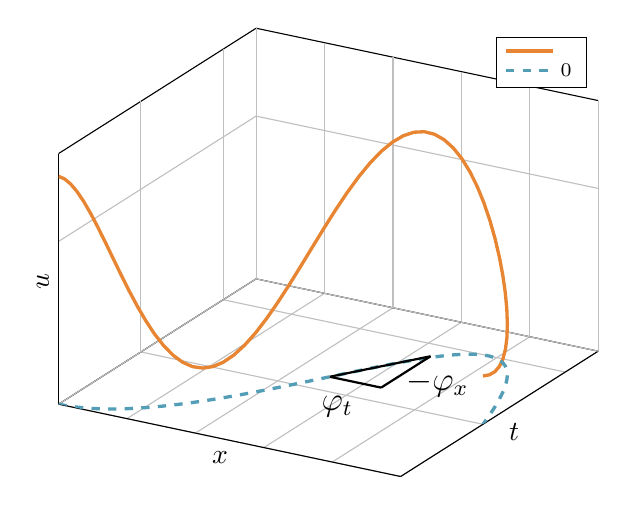
\begin{tikzpicture}
  \begin{axis}[view={30}{30},ticks=none,xlabel=$x$,ylabel=$t$,zlabel=$u$,zmin=0,ymax=5.2]
    \addplot3[Orange,very thick,domain=0:10,samples=60,samples y=0]
    ({x},
    {4+sin(1.5*x*x)},
    {4+3.*cos(deg(x))});
    \addplot3[Duck,dashed,very thick,domain=0:10,samples=60,samples y=0]
    ({x},{4+sin(1.5*x^2)},{0*x});
    \legend{$\Cscr$,$\Cscr_0$};
    % dt/dx = -phi_x/phi_t 
    \addplot3[thick]  coordinates {(5,4+sin(1.5*25),0) (6.5,4+sin(1.5*25),0)}  node[above] at (axis cs:6.9,4.05+0.6087-0.4,0.) {\large$\varphi_t$};
    \addplot3[thick]  coordinates {(5,4+sin(1.5*25),0) (6.5,4+sin(1.5*25)+0.3,0)};
    \addplot3[thick]  coordinates {(6.5,4+sin(1.5*25),0) (6.5,4+sin(1.5*25)+0.3,0)} node[right] at (axis cs:6.7,4.05+0.6087+0.,0.) {\large$-\varphi_x$};
  \end{axis}
\end{tikzpicture}
%%% Local Variables:
%%% mode: latex
%%% TeX-master: "../../mainManuscript"
%%% End:

  \caption{Example of curve initial curve $\Cscr$ in the $(x,t,u)$ space and its projection $\Cscr_0$ in the $(x,t)$ plane.}
  \label{fig:initial_curve}
\end{figure}
With data given along $\Cscr$, the Cauchy problem is equivalent to that of finding a surface $u(x,t)$ that contains the initial curve and satisfies \eqref{eq:1st_order_pde}. Thus, one seeks the derivatives of $u$ along $\Cscr$. Since $u=u(\varphi(x,t))$ along $\Cscr$, one has $u_x = u' \varphi_x $ and $u_t = u' \varphi_t$ from which one deduces:
\begin{equation*}
  u_t = \frac{\varphi_t}{\varphi_x}u_x 
\end{equation*}
This relation enables to rewrite the PDE \eqref{eq:1st_order_pde} as:
\begin{equation}
  \label{eq:normal_form_pde}
  (a + b\frac{\varphi_t}{\varphi_x})u_x = c
\end{equation}
On the other hand, the total differential of $\varphi(x,t)=const$ being $d\varphi = \varphi_x dx + \varphi_t dt =0$, equation \eqref{eq:normal_form_pde} becomes:
\begin{equation}
  \label{eq:normal_form_pde_2}
  (a - \ddroit{x}{t}b)u_x = c
\end{equation}
Hence, the Cauchy problem admits a unique solution if and only if:
\begin{equation}
  \label{eq:non-characteristics}
  \ddroit{x}{t}\neq \frac{a}{b}
\end{equation}
A \textit{non-characteristic curves} is an initial curve satisfying the condition \eqref{eq:non-characteristics}, otherwise it is a \textit{characteristic curve}. 

\subsubsection*{Geometrical representation of characteristic curves}
Let $u(x,t)$ be a surface in the $(x,t,u)$ space with normal vector is $\vect{n}=[u_x,u_t,-1]$. This surface is an integral surface if it is a solution of equation \eqref{eq:1st_order_pde} and hence, if $\vect{n}\cdot \vect{w}=0$ in $(x,t,u)$, where $\vect{w}=[a,b,c]$.
Figure \ref{fig:plan_fan} shows a collection of integral surfaces for some partial differential equation \eqref{eq:1st_order_pde} with prescribed $u$ along a straight line $\Cscr$. The set of tangent planes to every solutions $u^{(i)}(x,t)$ of equation \eqref{eq:1st_order_pde} thus forms a fan of planes which axis is $\vect{w}$.
% \begin{figure}[ht]
%   \centering
%   \subcaptionbox{Integral surfaces in $(x,t,u)$ space\label{subfig:fan_plan}}{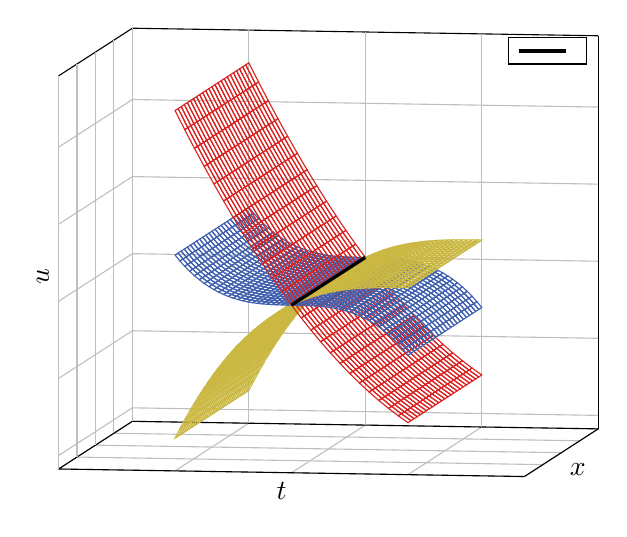
\begin{tikzpicture}
  \begin{axis}[view={99}{7},ticks=none,xlabel=$x$,ylabel=$t$,zlabel=$u$,ymin=-1.,ymax=1.]
    \addplot3[black,very thick,domain=-4:4,samples=60,samples y=0]({x},{0.},{5.});

    \addplot3[mesh,draw=Yellow,domain=-4:4,y domain=-0.5:0.] {2.*(y-0.5)^3+(2.*(0.5)^3)+5.};
    \addplot3[mesh,draw=Blue,domain=-4:4,y domain=-0.5:0.] {-5.*y^3+5.};
    \addplot3[mesh,draw=Red,domain=-4:4,y domain=-0.5:0.5] {2.*(y-1.)^2 -2. +5.};
    \addplot3[mesh,draw=Blue,domain=-4:4,y domain=-0.:0.5] {-5.*y^3+5.};
    \addplot3[mesh,draw=Yellow,domain=-4:4,y domain=-0.:0.5] {2.*(y-0.5)^3+(2.*(0.5)^3)+5.};
    \addplot3[black,very thick,domain=-4:4,samples=60,samples y=0]({x},{0.},{5.});
    \legend{$\Cscr$}
  \end{axis}
\end{tikzpicture}
%%% Local Variables:
%%% mode: latex
%%% TeX-master: "../../mainManuscript"
%%% End:
} \qquad 
%   \subcaptionbox{Projection in $(t,u)$ plane\label{subfig:fan_plan_proj}}{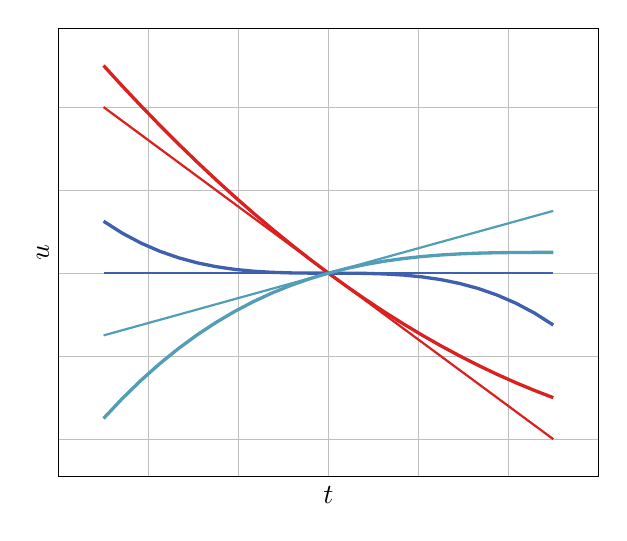
\begin{tikzpicture}
  \begin{axis}[ticks=none,xlabel=$t$,ylabel=$u$]
    \addplot[Red,very thick,domain=-0.5:0.5] {2.*(x-1.)^2 -2. +5.};
    \addplot[Red,thick,domain=-0.5:0.5] {-4.*x+5.};
    \addplot[Blue,very thick,domain=-0.5:0.5] {-5.*x^3+5.};
    \addplot[Blue,thick,domain=-0.5:0.5] {5.};
    \addplot[Duck,very thick,domain=-0.5:0.5] {2.*(x-0.5)^3+(2.*(0.5)^3)+5.};
    \addplot[Duck,thick,domain=-0.5:0.5] {1.5*x+5.};
    % \addplot3[black,very thick,domain=-5:5,samples=60,samples y=0]({x},{0.},{x^2+5.});
  \end{axis}
\end{tikzpicture}
%%% Local Variables:
%%% mode: latex
%%% TeX-master: "../../mainManuscript"
%%% End:
}
%   \caption{Examples of integral surfaces passing through the same initial curve $\Cscr$ defined such that $t=const$ and $u=const$ along $\Cscr$.}
%   \label{fig:plan_fan}
% \end{figure}
This defines \textit{characteristic line elements} tangent to all integral surfaces $u^{(i)}(x,t)$:
\begin{equation}
  \label{eq:monge_axis}
  \matrice{dx \\ dt \\ du} = \matrice{a \\ b \\c}
\end{equation}
\begin{figure}[h!]
  \centering
  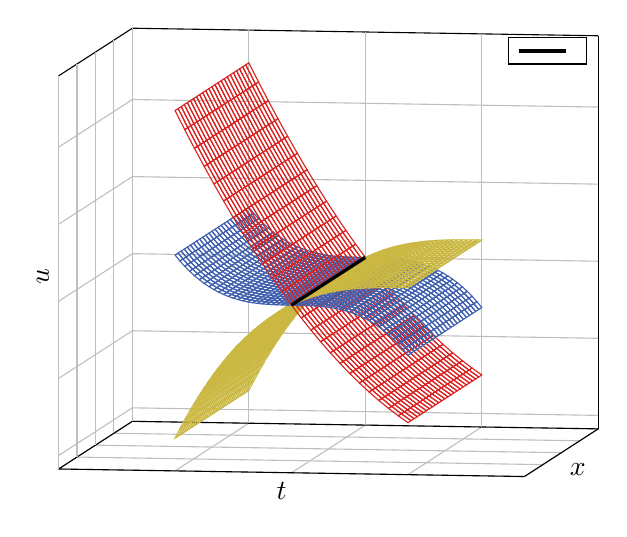
\begin{tikzpicture}
  \begin{axis}[view={99}{7},ticks=none,xlabel=$x$,ylabel=$t$,zlabel=$u$,ymin=-1.,ymax=1.]
    \addplot3[black,very thick,domain=-4:4,samples=60,samples y=0]({x},{0.},{5.});

    \addplot3[mesh,draw=Yellow,domain=-4:4,y domain=-0.5:0.] {2.*(y-0.5)^3+(2.*(0.5)^3)+5.};
    \addplot3[mesh,draw=Blue,domain=-4:4,y domain=-0.5:0.] {-5.*y^3+5.};
    \addplot3[mesh,draw=Red,domain=-4:4,y domain=-0.5:0.5] {2.*(y-1.)^2 -2. +5.};
    \addplot3[mesh,draw=Blue,domain=-4:4,y domain=-0.:0.5] {-5.*y^3+5.};
    \addplot3[mesh,draw=Yellow,domain=-4:4,y domain=-0.:0.5] {2.*(y-0.5)^3+(2.*(0.5)^3)+5.};
    \addplot3[black,very thick,domain=-4:4,samples=60,samples y=0]({x},{0.},{5.});
    \legend{$\Cscr$}
  \end{axis}
\end{tikzpicture}
%%% Local Variables:
%%% mode: latex
%%% TeX-master: "../../mainManuscript"
%%% End:

  \caption{Examples of integral surfaces passing through the same curve $\Cscr$ defined such that $t=const$ and $u=const$ along $\Cscr$.}
  \label{fig:plan_fan}
\end{figure}
Introduction of a parameter $\eta$ and integration of equation \eqref{eq:monge_axis} yields a one-parameter family of \textit{characteristic curves} of the PDE:
\begin{equation*}
  x=x(\eta) \quad ; \quad t=t(\eta) \quad ; \quad u=u(\eta)
\end{equation*}
Hence, a characteristic curve is tangent at every point to all the integral surfaces, and an infinity of integral surfaces cross one characteristic curve. As a consequence, if the initial curve is a characteristic curve, infinitely many integral surfaces contain it so that the Cauchy problem can not be solved.

However, the following statement holds \cite[Ch.1]{Courant}:
\begin{theorem}[Courant]
  \label{th:integral_surface_generated}
  Every surface $u(x,t)$ generated by a one-parameter family of characteristic curves is an integral surface. Conversely, every integral surface is generated by a one-parameter family of characteristic curves.
\end{theorem}
This theorem will be used in what follows to solve the Cauchy problem.

\subsection{The method of characteristic}
We now extend the concept of characteristic curves to first order quasi-linear systems of dimension $I$. In matrix form:
\begin{equation}
  \label{eq:1st_order_quasi-linear_syst}
  \Absf^t\(x,t,\vect{\Uc}\) \: \vect{\Uc}_t + \Absf^x\(x,t,\vect{\Uc}\)\: \vect{\Uc}_x + \vect{\Sc} = \vect{0}
\end{equation}
Similarly to quasi-linear PDEs, given values of $\Ucb$ are prescribed along a regular curve $\Cscr_0:\varphi(x,t)=const$ defining the initial curve $\Ucb(\varphi(x,t))$ of the $(x,t,\Ucb)$ space. The Cauchy problem consists in finding all the derivatives of $\Ucb(x,t)$ such that equation \eqref{eq:1st_order_quasi-linear_syst} is satisfied in the vicinity of $\Cscr$.
Noticing that along the initial curve $\Ucb_x = \Ucb' \varphi_x$ and $\Ucb_t = \Ucb' \varphi_t$, one gets:
\begin{equation*}
  \vect{\Uc}_x\varphi_t - \vect{\Uc}_t\varphi_x= \vect{0}
\end{equation*}
Hence, system \eqref{eq:1st_order_quasi-linear_syst} can be rewritten:
\begin{equation}
  \label{eq:normal_form}
  \( \Absf^x - \lambda \Absf^t \) \vect{\Uc}_x + \vect{\Sc} = \vect{0} 
\end{equation}
where:
\begin{equation}
  \label{eq:lambda_slope}
  \lambda=-\frac{\varphi_t}{\varphi_x}=\ddroit{x}{t}
\end{equation}
The Cauchy problem admits n unique solution $\vect{\Uc}_x$ along $\Cscr$ if the determinant of the system does not vanish, that is:
\begin{equation}
  \label{eq:characteristic_determinant}
  D=\abs{\Absf^x - \lambda \Absf^t} \ne 0
\end{equation}
where D is called the \textit{characteristic determinant} of system \eqref{eq:1st_order_quasi-linear_syst}. If D does not have real roots along $\Cscr_0$, the problem is said \textit{elliptic} and the Cauchy problem can be solved. Indeed, in that case the knowledge of $\Ucb$ along the initial curve allows the computation of derivatives and hence, the building of an integral strip defined by $\Ucb,\Ucb_x,\Ucb_t$. If equation \eqref{eq:1st_order_quasi-linear_syst} admits $I$ real roots on the other hand, system \eqref{eq:normal_form} can no longer be solved. Those eigenvalues come along with left and right eigenvectors respectively defined as:
\begin{equation}
  \label{eq:eigenvectors}
  \Lc^k_i  \Asf^x_{ij} = \lambda_k \Lc^k_i \Asf^t_{ij} \quad ; \quad \Asf^x_{ij}\Rc^k_j = \lambda_k \Asf^t_{ij}\Rc^k_j \qquad k=1,...,I
\end{equation}
\begin{remark}
  Note that eigenvectors can be stored as matrices $\Rbsf$ and $\Lbsf$ where $\Rsf_{ij}=\Rc^j_i$ and $\Lsf_{ij}=\Lc_j^i$.
\end{remark}

A first order system of $I$ partial differential equations is said \textit{hyperbolic} if it admits $I$ real eigenvalues associated to independent eigenvectors \cite{Courant}.
For those problems one can draw a set of one-parameter families of curves in the $(x,t)$ plane by integrating the relations $\lambda_k=dx/dt$ ($1 \leq k \leq I$).
\begin{example}
  \label{ex:charac1}
  Consider the first order system with variable coefficients
\begin{equation*}
 \matrice{x &0 \\0 &-x} \drond{}{t} \matrice{\Uc_1 \\ \Uc_2} + \drond{}{x}\matrice{\Uc_1 \\ \Uc_2} = \matrice{0 \\0}
\end{equation*}
which characteristic determinant \eqref{eq:characteristic_determinant} is:
\begin{equation*}
  (1-\lambda x)(1+\lambda x)=0
\end{equation*}
We thus have two solutions $\lambda_{1,2}=\pm 1/x$ leading, by integration of \eqref{eq:lambda_slope}, to two one-parameter families of characteristic curves:
\begin{equation*}
  t_1(x)=\frac{1}{2}x^2+c_1  \quad \text{and} \quad t_2(x)=-\frac{1}{2}x^2+c_2 
\end{equation*}
Those curves are drawn in figure \ref{fig:exampleCharac}\subref{subfig:curve_lines} for several values of integration constants $c_1$ and $c_2$.
\end{example}
\begin{example}
  \label{ex:charac2}
  Consider now the first order system with constant coefficients
\begin{equation*}
 \matrice{1 &0 \\0 &2} \drond{}{t} \matrice{\Uc_1 \\ \Uc_2} + \drond{}{x}\matrice{\Uc_1 \\ \Uc_2} = \matrice{0 \\0}
\end{equation*}
which eigenvalues, according to equation \eqref{eq:characteristic_determinant} satisfy
\begin{equation*}
  (1 - \lambda )(1- 2\lambda)=0
\end{equation*}
Two real roots exist $\lambda_1=1 \: ; \: \lambda_2=1/2$, leading by integration of \eqref{eq:lambda_slope} to two one-parameter families of straight lines:
\begin{equation*}
  t_1(x)=x+c_1  \quad \text{and} \quad t_2(x)=2x+c_2 
\end{equation*}
Unlike example \ref{ex:charac1}, coefficient matrices do not depend on independent variables, thus yielding to characteristic straight lines in the $(x,t)$ plane (see \ref{fig:exampleCharac}\subref{subfig:straight_lines}).
\end{example}
\begin{figure}[h]
  \centering
  \subcaptionbox{Example \ref{ex:charac1}: $\lambda_{1,2}=\pm 1/x$\label{subfig:curve_lines}}{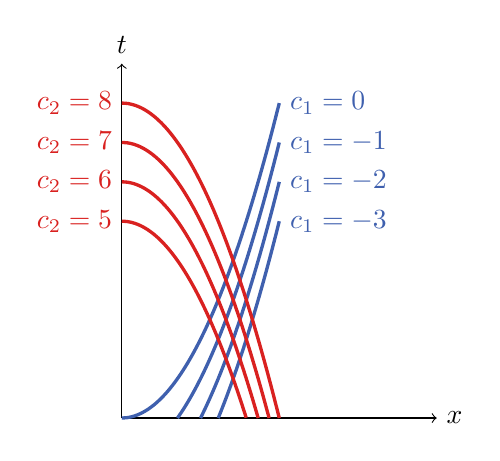
\begin{tikzpicture}
  \draw[->] (0,0) -- (4.,0) node[right] {$x$};
  \draw[->] (0,0) -- (0,4.5) node[above] {$t$};
  \draw[scale=0.5,domain=0:4,smooth,variable=\x,Blue,very thick] plot ({\x},{0.5*\x*\x}) node [right] {$c_1=0 $};
  \draw[scale=0.5,domain=1.4142:4,smooth,variable=\x,Blue,very thick] plot ({\x},{0.5*\x*\x-1}) node [right] {$c_1=-1$};
  \draw[scale=0.5,domain=2:4,smooth,variable=\x,Blue,very thick] plot ({\x},{0.5*\x*\x-2}) node [right] {$c_1=-2$};
  \draw[scale=0.5,domain=2.44948:4,smooth,variable=\x,Blue,very thick] plot ({\x},{0.5*\x*\x-3}) node [right] {$c_1=-3$};
  \draw[scale=0.5,domain=0:3.16,smooth,variable=\x,Red,very thick] plot ({\x},{-0.5*\x*\x+5});
  \node[left,Red] at (0,2.5) {$c_2=5$};
  \draw[scale=0.5,domain=0:3.4641,smooth,variable=\x,Red,very thick] plot ({\x},{-0.5*\x*\x+6});
  \node[left,Red] at (0,3) {$c_2=6$};
  \draw[scale=0.5,domain=0:3.7416,smooth,variable=\x,Red,very thick] plot ({\x},{-0.5*\x*\x+7});
  \node[left,Red] at (0,3.5) {$c_2=7$};
  \draw[scale=0.5,domain=0:4,smooth,variable=\x,Red,very thick] plot ({\x},{-0.5*\x*\x+8});
  \node[left,Red] at (0,4) {$c_2=8$};
\end{tikzpicture}
%%% Local Variables:
%%% mode: latex
%%% TeX-master: "../../mainManuscript"
%%% End:
}
  \subcaptionbox{Example \ref{ex:charac2}: $\lambda_{1}=1 \:\text{and} \: \lambda_2=1/2$\label{subfig:straight_lines}}{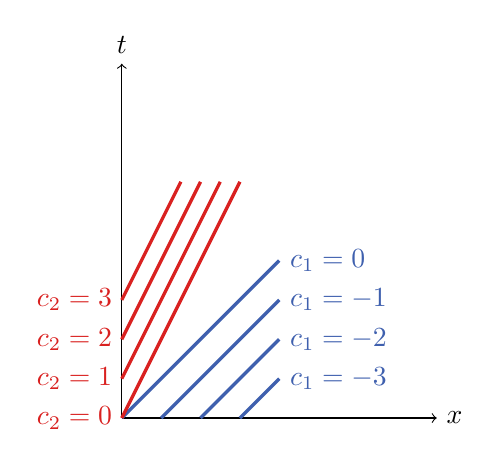
\begin{tikzpicture}
  \draw[->] (0,0) -- (4.,0) node[right] {$x$};
  \draw[->] (0,0) -- (0,4.5) node[above] {$t$};
  \draw[scale=0.5,domain=0:4,smooth,variable=\x,Blue,very thick] plot ({\x},{\x}) node [right] {$c_1=0$};
  \draw[scale=0.5,domain=1.:4,smooth,variable=\x,Blue,very thick] plot ({\x},{\x-1}) node [right] {$c_1=-1$};
  \draw[scale=0.5,domain=2:4,smooth,variable=\x,Blue,very thick] plot ({\x},{\x-2}) node [right] {$c_1=-2$};
  \draw[scale=0.5,domain=3:4,smooth,variable=\x,Blue,very thick] plot ({\x},{\x-3}) node [right] {$c_1=-3$};
  \draw[scale=0.5,domain=0:3,smooth,variable=\x,Red,very thick] plot ({\x},{2*\x});
  \node[left,Red] at (0,0) {$c_2=0$};
  \draw[scale=0.5,domain=-0.:2.5,smooth,variable=\x,Red,very thick] plot ({\x},{2*\x+1});
  \node[left,Red] at (0,0.5) {$c_2=1$};
  \draw[scale=0.5,domain=-0:2,smooth,variable=\x,Red,very thick] plot ({\x},{2*\x+2});
  \node[left,Red] at (0,1) {$c_2=2$};
  \draw[scale=0.5,domain=-0:1.5,smooth,variable=\x,Red,very thick] plot ({\x},{2*\x+3});
  \node[left,Red] at (0,1.5) {$c_2=3$};
\end{tikzpicture}
%%% Local Variables:
%%% mode: latex
%%% TeX-master: "../../mainManuscript"
%%% End:
}
  \caption{Family of base characteristic curves corresponding to the eigenvalues of the first order systems given in examples \ref{ex:charac1} and \ref{ex:charac2}.}
  \label{fig:exampleCharac}
\end{figure}

As theorem \ref{th:integral_surface_generated} states, an integral surface is generated by a one-parameter family of characteristic curves. Therefore the knowledge of those curves can be used to build the solution of the Cauchy problem. Indeed, the projection of the quasi-linear system \eqref{eq:1st_order_quasi-linear_syst} onto the \textit{left eigenbasis} or \textit{left characteristic basis} leads to:
\begin{equation*}
  \vect{\Lc}^k \( \Absf^t \vect{\Uc}_t + \Absf^x\vect{\Uc}_x \) + \vect{\Lc}^k \vect{\Sc}= \vect{0}
\end{equation*}
%Introduction of the definition of left eigenvectors \eqref{eq:eigenvectors} then yields:
where $\Lcb^k$ satisfies \eqref{eq:eigenvectors}, and hence:
\begin{equation*}
  \vect{\Lc}^k  \Absf^t \( \vect{\Uc}_t +\lambda_k \vect{\Uc}_x   \) + \vect{\Lc}^k \vect{\Sc}=\vect{0}
\end{equation*}
In this equation, the \textit{directional derivative} of $\vect{\Uc}$ along the $k$th characteristic curve arises, namely:
\begin{equation*}
 \ddroit{\Ucb}{t}\lvert_{t\in\varphi^k} = \Ucb_t + \lambda_k \Ucb_x   
\end{equation*}
Thus, along a characteristic curve a system of partial differential equations reduces to a system of \textit{Ordinary Differential Equations} (ODEs) composed of the following \textit{characteristic equations}:
\begin{equation}
  \label{eq:PDEs_ODEs}
  \vect{\Lc}^k  \Absf^t \(\ddroit{\Ucb}{t} + \Scb \)=\vect{0}
\end{equation}
Integration of equations \eqref{eq:PDEs_ODEs} yields a set of \textit{integral curves} from which the Cauchy problem can be solved.
%It then comes out that the Cauchy problem can be solved as the system \eqref{eq:PDEs_ODEs}.
Indeed, the solution at a point of the $(x,t)$ plane can be determined by tracing backward the characteristic curves to the initial curve and integrating ODEs \eqref{eq:PDEs_ODEs} along those paths according to the \textit{method of characteristics}. Note that if the right-hand side of equation \eqref{eq:1st_order_quasi-linear_syst} is zero, then $\Ucb$ is constant along characteristic curves. 

To illustrate the method, let us consider again the quasi-linear system of example \ref{ex:charac1} for which the Cauchy problem is built by prescribing initial conditions along the $x$-axis. Note that "initial conditions" have now a physical meaning since they are defined at $t=0$, the Cauchy problem is then an \textit{Initial Value Problem (IVP)}. Through a point $(x^*,t^*)$ pass two characteristic curves, each belonging to a different one-parameter family. The solution at this point can be determined by integrating the ODE corresponding to the first (\textit{resp. second}) eigenvalue of the system between $(x^1,0)$ (\textit{resp. $(x^2,0)$}) and $(x^*,t^*)$. The singularity of hyperbolic problems can hence be circumvented by using the characteristic structure in order to determine n unique solution. 
\begin{figure}[h]
  \centering
  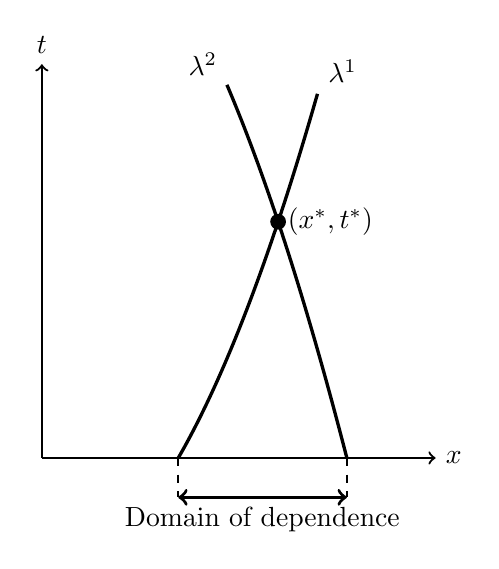
\begin{tikzpicture}
  \draw[thick,->](0,0)--(5,0) node [right] {$x$};
  \draw[thick,->](0,0)--(0,5) node [above] {$t$};
  % t1 = 0.5*x**2 + c1
  % t2 = -0.5*x**2 + c2
  % -> c1 = -1.5 ; c2 = 7.5
  % \draw[domain=1.7320508:3.5,smooth,variable=\x,Purple,very thick] plot ({\x},{0.5*\x*\x-1.5}) node [above right] {$t=\frac{x^2-3}{2}$};
  % \draw[domain=2.35:3.872983,smooth,variable=\x,Green,very thick] plot ({\x},{-0.5*\x*\x+7.5});
  \draw[domain=1.7320508:3.5,smooth,variable=\x,very thick] plot ({\x},{0.5*\x*\x-1.5}) node [above right] {$\lambda^1$};
  \draw[domain=2.35:3.872983,smooth,variable=\x,very thick] plot ({\x},{-0.5*\x*\x+7.5});
  % \node[left,Green] at (2.35,5) {$t=-\frac{x^2-15}{2}$};
  \node[left] at (2.35,5) {$\lambda^2$};
  \draw[<->,very thick] (1.7320508,-0.5) -- (3.872983,-0.5) ;
  \draw[dashed,thick] (1.7320508,0) -- (1.7320508,-0.5);
  \draw[dashed,thick] (3.872983,-0.) -- (3.872983,-0.5);
  \node[below] at (2.80,-0.5) {\text{Domain of dependence}};
  \fill[black] (3,3) circle (0.1) node [right] {$(x^*,t^*)$};
\end{tikzpicture}
%%% Local Variables:
%%% mode: latex
%%% TeX-master: "../../mainManuscript"
%%% End:

  \caption{Domain of dependence of the solution at point $(x^*,t^*)$ for the system of example \ref{ex:charac1}.}
  \label{fig:charac_method2x2}
\end{figure}
We see that only a segment of the initial curve has an influence on the solution at a given point. Namely, the intersections of the initial curve and characteristic curves with the highest and the lowest slopes define the \textit{domain of dependence} of the solution at this point (see figure \ref{fig:charac_method2x2}). This property of hyperbolic problems implies the existence of waves that propagates information at finite speeds corresponding to the eigenvalues of a quasi-linear form. The theory presented so far will be applied in what follows to solid mechanics.



%%% Local Variables:
%%% mode: latex
%%% TeX-master: "../mainManuscript"
%%% End:


\section{Conservation laws in solid mechanics}
\label{sec:solidMech_equations}
%In this section, the mathematical laws allowing the description of the deformation of a solid body will be derived. First, the kinematic laws governing the motion of each material point belonging to a solid will be considered. The variations of lengths and shapes of a continuum, described by the \textit{strain} mesure will then be associated to internal forces through thermodynamic framework. Finally, the theory of first order quasi-linear partial differential system will be applied to solid dynamics in order to deliver analytical solutions for specific problems. The literature on the subject being very rich (see for instance \cite[Chapters~1-3]{Foundation_of_elasticity}, \cite{Truesdell}, \cite[Chapter~7]{Simo}, \cite[Chapters~3 \& 5]{Belytschko}), the governing equations of mechanics will be developed non-exhaustively.

\subsection{Kinematic laws -- Strain mesures}
We consider a three-dimensional solid domain with volume denoted by $\Omega \subset \Rbb^3$ bounded by the surface $\partial \Omega$. This body undergoes external sollicitations that can either be localized on a part of the external surface of the body (\textit{i.e. surface forces}) or act in the whole solid domain (\textit{i.e. volume forces}). Due to the presence of such sollicitations, the volume may change during a deformation within the time interval $\tau = \[0,T\]$ and will hence be written as a function of time $\Omega(t)$ ($t\in \tau$). The state of the solid at time $t=0$, corresponding to a non-deformed state with volume $\Omega(t=0)=\Omega_0$, is referred to as the \textit{initial configuration}. Some problems require the use of a \textit{reference configuration} that can be deformed and to which equations are referred. In what follows, the reference and initial conditions are identical. At a given time $t>0$, the volume $\Omega(t)=\Omega_t$ corresponds to the \textit{current configuration}. These configurations are depicted in figure \ref{fig:deformationFunction}.
\begin{figure}[h]
  \centering
  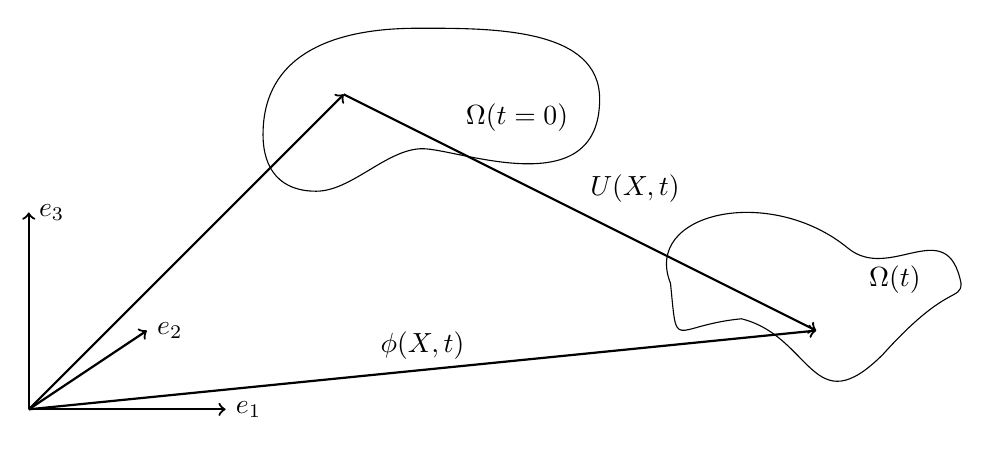
\begin{tikzpicture}
  %\draw[step=1.0,black,thin] (-3.,-1.) grid (3,4.);
  %\draw (-3,-1) -- (3,-1) -- (3,4) -- (-3,4) -- (-3,-1);
  \draw[thick,->] (-5,-2.5) -- (-2.5,-2.5) node [right] {$\vect{e}_1$};
  \draw[thick,->] (-5,-2.5) -- (-5,0.) node [right] {$\vect{e}_3$};
  \draw[thick,->] (-5,-2.5) -- (-3.5,-1.5) node [right] {$\vect{e}_2$};
  \begin{scope}[scale=0.45]
    \draw (-3,0.6) .. controls +(1,0) and +(-1,0) .. (0,1.8)  
    .. controls +(1,0) and +(0,-3) .. (5,3.2) 
    .. controls +(0,2) and +(2,0)  .. (0,5.2) 
    .. controls +(-1,0) and +(0,3) .. (-4.5,2.2) 
    .. controls +(0,-1) and +(-1,0).. (-3,0.6) ;
  \end{scope}
  \node at (1.2,1.2) {$\Omega(t=0)$};
  %% Deformed body +2.
  \begin{scope}[scale=0.9]
    \draw (0.+0.5+4.,0-1.5) ..controls (1.+0.5+4.,-0.25-1.5) and (1.+0.5+4.,-1.5-1.5) .. (2.+0.5+4.,-0.5-1.5) ..controls (2.9+0.5+4.,0.5-1.5) and (3.1+0.5+4.,0.25-1.5) .. (3.1+0.5+4.,0.5-1.5) ..controls (2.9+0.5+4.,1.5-1.5) and (2.1+0.5+4.,.5-1.5) .. (1.5+0.5+4.,1.-1.5) ..controls (0.4+0.5+4.,1.9-1.5) and (-1.4+0.5+4.,1.5-1.5) .. (-1.+0.5+4.,0.5-1.5)..controls (-0.4+0.+4.,-0.-2.) and (-1+0.5+4.,0.4-2.) .. (0+0.5+4.,0-1.5);
  \end{scope}
  \node at (6.,-0.85) {$\Omega(t)$};
  \draw[->,thick] (-5,-2.5) -- (-1.,1.5) node [midway,left] {$\X$};
  \draw[->,thick] (-5,-2.5) -- (5.,-1.5) node [midway,above] {$\vect{\phi}(\vect{X},t)$};
  \draw[->,thick] (-1.,1.5) -- (5.,-1.5) node [midway,above right] {$\vect{U}(\vect{X},t)$};
\end{tikzpicture}

%%% Local Variables:
%%% mode: latex
%%% TeX-master: "../../mainManuscript"
%%% End:
  \caption{Deformation of a solid body between a reference state $\Omega_0$ to a subsequent state $\Omega_t$.}
  \label{fig:deformationFunction}
\end{figure}

In the reference configuration, every material particle is located by their position vectors: $\vect{X}=X_\alpha \vect{e}_\alpha$, where $X_\alpha$ denotes the \textit{Lagrangian coordinates} and $\vect{e}_\alpha$ the basis vectors. At a subsequent time $t$, the particle initially located at $\vect{X}$ may have moved and its current location is given by the smooth mapping $\vect{\phi}(\vect{X},t)=\phi_i(\vect{X},t)\vect{e}_i$. Thus, the mapping $\vect{\phi}$ provides the paths of every particle of the solid during the deformation. In the lagrangian coordinates system, every particles are tracked during the deformation while the \textit{Eulerian coordinates}, denoted by $\vect{x}=x_i\vect{e}_i$, correspond to a \textit{spatial description}.
Note that in the above definitions Greek indices are used for quantities evaluated in the reference configuration whereas Latin ones refer to quantities defined in the current configuration. 

The \textit{displacement} and \textit{velocity} vectors of a particle between the reference and the current configuration are respectively:
\begin{subequations}
  \begin{alignat}{2}
    &\vect{u}(\vect{X},t)=\vect{\phi}(\vect{X},t) - \vect{X} \qquad \forall\:\: \vect{X},t \in \Omega_0\times \tau  \label{eq:displacement}\\
    &\vect{v}(\vect{X},t)=\drond{\vect{\phi}}{t}(\vect{X},t) = \vect{\dot{\phi}}(\vect{X},t) \qquad  \forall\: \: \vect{X},t \in \Omega_0\times \tau  \label{eq:velocity}
  \end{alignat}
\end{subequations}
where the superposed dot denotes the material time derivative. Then, the second-order two-point \textit{deformation gradient} tensor is defined as:
\begin{equation}
  \label{eq:F_phi}
    \tens{F}=\nablat_0 \vect{\phi} (\vect{X},t)
\end{equation}
where $\nablat_0 (\bullet)$ refers to the gradient operator on the reference configuration. This tensor can also be written by using equation \eqref{eq:displacement}:
\begin{equation}
  \tens{F}= \nablat_0 \vect{u}(\vect{X},t) + \tens{I} \label{eq:F_displacement}
\end{equation}
with $\tens{I}$, the second-order identity tensor. The deformation gradient tensor characterizes the variations of lengths, areas and volumes. Indeed, the infinitesimal vector, oriented surface and volume elements respectively denoted by $\vect{dX},\vect{dS}$ and $dV$ and defined in the reference configuration transorm respectively to:
\begin{equation}
  \label{eq:transport_equations}
  \begin{aligned}
    & dx_i=F_{i\alpha}dX_\alpha \\
    & ds_i=J F_{\alpha i}^{-1}dS_{\alpha} \\
    & dv=JdV 
  \end{aligned}
\end{equation}
in the current configuration. The transport equations \eqref{eq:transport_equations} involve the determinant of the deformation gradient $J=\det(\tens{F})>0$, also called the \textit{Jacobian of the deformation}. The deformation gradient is a strain mesure since it accounts for changes in lengths and angles (\textit{i.e. the change of shape of a body}). Other strain mesures can be used as the \textit{right Cauchy-Green} or the \textit{Green-Lagrange} tensors, respectively defined as:
\begin{equation*}
  \begin{aligned}
    & \tens{C}=\tens{F}^T\tens{F} \\
    & \tens{E}=\frac{1}{2}(\tens{C}-\tens{I})
  \end{aligned}
\end{equation*}
where $\tens{I}$ is the second-order identity tensor. The Green-Lagrange tensor can also be written by means of equation \eqref{eq:F_displacement}:
\begin{equation*}
  \tens{E}=\frac{1}{2}(\nablat_0 \vect{u} + \nablat_0 \vect{u}^T + \nablat_0 \vect{u}\nablat_0 \vect{u}^T)
\end{equation*}
In particular, when the deformation involves displacement vectors such that $\norm{\nablat_0 \vect{u}} \ll 1$, the last (second-order) term of the previous definition can be neglected leading to:
\begin{equation*}
  \tens{E} \approx \frac{1}{2}(\nablat_0 \vect{u} + \nablat_0 \vect{u}^T) = \tens{\eps}
\end{equation*}
with $\tens{\eps}$ the \textit{linearized strain tensor}, the symmetric part of the displacement gradient. Such deformations fall in the \textit{linearized geometrical framework} and are characterized by small strain but possibly large displacements. Furthermore, when the deformation leads to a displacement vector $\norm{\vect{u}} \ll 1$ reference and current configurations are considered as indentical. These situations correspond to the \textit{small strain} framework for which the reference and current configurations are considered as identical.

\subsection{Balance equations}
In this section a solid domain $\Omega(t)$ undergoing a deformation is still considered within the time interval $\tau = \[0,T\]$. We start the development of balance laws that hold in the continuum during the deformation by the conservation of mass of a conntinuum, which in integral form reads:
\begin{equation*}
  \int_\Omega \rho d\Omega = \int_{\Omega_0} \rho_0 d\Omega \qquad \forall \: t \in  \tau
\end{equation*}
which, with the third transport formula reads:
\begin{equation}
  \label{eq:mass_conservation_law}
  \int_{\Omega_0} \(J\rho - \rho_0\) d\Omega = 0
\end{equation}
Leading to the first balance equation, namely the local conservation of mass:
\begin{equation}
  \label{eq:mass_balance}
  \rho = \frac{\rho_0}{J} \qquad \forall \: \vect{X},t \: \in \Omega_0\times \tau
\end{equation}

We now move on to the equilibrium between acceleration effects, namely \textit{intertia}, and external forces undergone by a solid $\Omega$. This conservation law corresponds to \textit{Newton's second law}:
\begin{equation*}
  \int_\Omega \rho \vect{\dot{v}} d\Omega = \int_{\partial \Omega} \vect{t} dS + \int_{\Omega} \rho\vect{b}d\Omega \qquad \forall \: t \in  \tau
\end{equation*}
where $\vect{t}$ denotes surface forces and $vect{b}$ volume forces in the current configuration. We then introduce the symetric second-order \textit{Cauchy stress tensor} $\tens{\sigma}$ by using Cauchy's theorem $\vect{t}=\tens{\sigma}\cdot \vect{n}$ where $\vect{n}$ is the outwerd normal vector to the surface element $dS$. 

For further developments, the divergence theorem is required:
\begin{equation}
  \label{eq:Ostrogradski_th}
  \int_{\partial \Omega} (\bullet)\cdot \vect{dS}=\int_\Omega \nablav \cdot (\bullet) \: d\Omega
\end{equation}
where $\nablav \cdot (\bullet)$ denotes the divergence operator on the current configuration. Introduction of the previous formula in the second law of Newton leads to:
\begin{equation}
  \label{eq:Linear_momentum_conservation_eulerian}
  \int_{\Omega} \( \rho \vect{\dot{v}} - \nablav \cdot \tens{\sigma} -  \rho\vect{b} \) d\Omega = \vect{0} \qquad \forall \:t \in  \tau
\end{equation}
Conservation law \eqref{eq:Linear_momentum_conservation_eulerian} can be mapped to the reference configuration by using the transport formula of volume elements and the mass balance equation \eqref{eq:mass_balance}, thus yielding:
\begin{equation}
  \label{eq:Linear_momentum_conservation}
  \int_{\Omega_0} \( \rho_0 \vect{\dot{v}} - J \nablav \cdot \tens{\sigma} -  \rho_0\vect{b} \) d\Omega = \vect{0} \qquad \forall \: t \in\tau
\end{equation}
In equation \eqref{eq:Linear_momentum_conservation}, the divergence operator on the current configuration can be transported to the reference one by means of the \textit{Piola transform}:
\begin{definition}
  The Piola--Kirchhoff tranform $\tens{T}^P$ of a second-order tensor $\tens{T}$ is defined as:
  \begin{equation*}
    \tens{T}^P=J\tens{T}\cdot\tens{F}^{-1}
  \end{equation*}
  and satisfies:
  \begin{equation*}
    \nablav_0\cdot \tens{T}^P = J \nablav \cdot \tens{T}
  \end{equation*}
  where $\nablav_0\cdot (\bullet)$ is the divergence operator on the reference configuration.
\end{definition}
Another stress mesure that corresponds to the Piola transform of Cauchy stress tensor is thus introduced, the \textit{first Piola-Kirchhoff stress tensor} $\tens{\Pi}=J\tens{\sigma}\cdot\tens{F}^{-1}$. Hence, the vanishing of the integrand in equation \eqref{eq:Linear_momentum_conservation} yields the balance equation of the \textit{lagrangian linear momentum}:
\begin{equation}
  \label{eq:Lagrangian_linear_momentum}
  \rho_0 \vect{\dot{v}} - \nablav_0 \cdot \tens{\Pi} = \rho_0 \vect{b} \qquad \forall \: \: \vect{X},t \in \Omega_0 \times \tau 
\end{equation}
When considering deformations within the small strain framework the balance equation of linear momentum can be deduced from equation \eqref{eq:Linear_momentum_conservation_eulerian}, leading to:
\begin{equation}
  \label{eq:HPP_linear_momentum}
  \rho \vect{\dot{v}} - \nablav \cdot \tens{\sigma} = \rho \vect{b}  \qquad \forall \: \: \vect{x},t \in \Omega \times \tau 
\end{equation}

We complete the set of balance laws by considering the conservation of the energy of a system, also known as the \textit{first law of thermodynamics}. This law relates a balance between the rates of change of \textit{kinetic} and \textit{internal} energies, the power of external forces and the amount of heat entering the system as \textit{volume} or \textit{surface heat sources}.
\begin{equation*}
  \ddroit{}{t}\int_{\Omega} \(\frac{1}{2}\rho \vect{v}\cdot\vect{v} + \rho e\) d\Omega = \int_{\partial \Omega} \(\tens{\sigma}\cdot\vect{n}\)\cdot\vect{v} \: dS + \int_{\Omega} \rho\vect{b}\cdot\vect{v} \: d\Omega + \int_{\Omega} \rho r \:d\Omega - \int_{\partial \Omega} \vect{q}\cdot\vect{n} \: dS \qquad \forall \: t \in  \tau 
\end{equation*}
where $\vect{q}$ is the outward heat flux vector and $r$ is a volume heat source. By using the divergence theorem \eqref{eq:Ostrogradski_th}, the previous equation reads:
\begin{equation*}
\ddroit{}{t}\int_{\Omega} \(\frac{1}{2}\rho \vect{v}\cdot\vect{v} + \rho e\) d\Omega = \int_{\Omega} \(\nablav\cdot(\tens{\sigma}\cdot\vect{v}) +  \rho\vect{b}\cdot\vect{v} \) d\Omega + \int_{\Omega} \rho r \: d\Omega  - \int_{\partial \Omega} \vect{q}\cdot\vect{n} \: dS \qquad \forall \: t \in  \tau 
\end{equation*}
The transport of this relation on the reference configuration based on \eqref{eq:transport_equations} allows to introduce the time derivative of the left-hand side in the integral
\begin{equation*}
\int_{\Omega_0} \(\rho_0 \vect{\dot{v}} + \rho_0 \dot{e}\) d\Omega = \int_{\Omega_0} \(J\nablav\cdot(\tens{\sigma}\cdot\vect{v}) +  \rho_0\vect{b}\cdot\vect{v} \) d\Omega + \int_{\Omega_0} \rho_0 r \:d\Omega- \int_{\partial \Omega_0} J\vect{q}\cdot \tens{F}^{-1}\cdot\vect{n} \: dS \qquad \forall \: t \in  \tau 
\end{equation*}
Then, substitution of the linear momentum according to equation \eqref{eq:Lagrangian_linear_momentum} yields, after some algebra, the conservation law of internal energy:
\begin{equation}
  \label{eq:conservation_law_energy}
  \int_{\Omega_0} \rho_0 \dot{e} d\Omega = \int_{\Omega_0} \tens{\Pi}:\nablat_0\vect{v}\: d\Omega + \int_{\Omega_0} \(\rho_0r  - \nablav_0 \cdot \vect{Q}\) d\Omega \qquad \forall \: t \in  \tau 
\end{equation}
where $\vect{Q}=J\vect{q}\cdot \tens{F}^{-1}$ is the lagrangian heat flux vector. We thus deduce the balance equation of internal energy on the reference configuration:
\begin{equation}
  \label{eq:energy_balance}
  \rho_0 \dot{e} -  \tens{\Pi}:\nablat_0\vect{v}  + \nablav_0 \cdot \vect{Q}  = r \qquad \forall \: \: \vect{X},t \in \Omega_0 \times \tau 
\end{equation}
where $\nablat_0\vect{v} = \tens{\dot{F}}$. Finally, the small strain version of equation \eqref{eq:energy_balance} is: 
\begin{equation}
  \label{eq:energy_balance}
  \rho \dot{e} -  \tens{\sigma}:\nablat^{s} \vect{v}  + \nablav \cdot \vect{q}  = r \qquad \forall \: \: \vect{x},t \in \Omega \times \tau 
\end{equation}
in which $\nablat^{s} (\bullet)$ denotes the symetric part of the gradient, in particular: $\nablat^s \vect{v} = \tens{\dot{\eps}}$. Stress mesures are conjugate to strain mesures through the power. In what follows, stress and strain may respectively be refered to as \textit{thermodynamic forces} and \textit{internal variables} according to the thermodynamics framework. The former obey a \textit{state equation} while the latter describe the evolution of the thermodynamic system. 
\subsection{Constitutive equations}
The closure of a problem is given by the constitutive equations (\textit{i.e state laws}) for the stress. Once and for all, we consider here constitutive models within the \textit{Generalized Standard Materials} (GSM) framework \cite{GSM}.

\subsubsection*{The general (hyper)elasticity formulation}
First, the \textit{Clausius-Duhem} inequality resulting from combination of first and second laws of thermodynamics, reads: 
\begin{equation}
  \label{eq:Clausius-Duhem}
  \underbrace{\phantom{\frac{1}{\theta}} \tens{\Pi}:\tens{\dot{F}} + \rho_0 \(\theta \dot{\eta} -\dot{e}\)}_{\Dc^{int}} \:-\:  \underbrace{\frac{1}{\theta} \vect{q} \cdot \nablav_0 \theta}_{-\Dc^{th}} \geq 0  \qquad \forall \: \: \vect{X},t \in \Omega_0 \times \tau 
\end{equation}
where $\Dc^{int}$ and $\Dc^{th}$ are respectively the specific mechanical and thermal dissipations, and $\eta, \theta$ denote \textit{entropy} and \textit{temperature}. Equation \eqref{eq:Clausius-Duhem} results in vanishing dissipations for \textit{reversible} processes and in a strict inequality for \textit{irreversible} ones. Furthermore, a widely used assumption consists in considering that the mechanical and thermal dissipations simultaneously satisfy non-negativeness. Note that the \textit{Fourier's law} of conduction is based on the non-negativeness of the thermal dissipation and leads to the following definition of the heat flux vector in order to ensure the positivity of the thermal dissipation:
\begin{equation*}
  \label{eq:Fourier_law}
  \vect{q}=-\tens{k}\cdot\nablav_0 \theta
\end{equation*}


We assume the existence of a \textit{Helmholtz free energy density potential} $\psi\(\tens{F},\theta,V_p\)$ where the $V_p$ $(1\leq p \leq N)$ are additional state variables describing irreversible processes. The free energy is supposed concave with respect to temperature and convex with respect to other variables. The mechanical dissipation then can be rewritten as:
\begin{equation*}
  \Dc^{int} = \tens{\Pi}:\tens{\dot{F}} - \rho_0 \(\dot{\psi} +\eta \dot{\theta}\) 
\end{equation*}
The time derivative of Helmholtz free energy:
\begin{equation*}
  \dot{\psi} = \drond{\psi}{\tens{F}}:\tens{\dot{F}} + \drond{\psi}{\theta}\dot{\theta} + \drond{\psi}{V_p}\dot{V_p}
\end{equation*}
can be introduced within the mechanical dissipation so that one gets:
\begin{equation}
  \label{eq:Dint_psi_factor}
  \Dc^{int} = \(\tens{\Pi}- \rho_0 \drond{\psi}{\tens{F}} \):\tens{\dot{F}} - \rho_0 \(\drond{\psi}{\theta} +\eta\) \dot{\theta}  - \rho_0\drond{\psi}{V_p}\dot{V_p} 
\end{equation}


Since the mechanical dissipation must be non-negative regardless of the nature of the deformation, it must in particular vanish for a reversible isothermal process (\textit{i.e. $\theta=const$}) for which every additional internal variables are constant. With these considerations, we are left with the relation:
\begin{equation*}
  \( \tens{\Pi} - \rho_0\drond{\psi}{\tens{F}} \): \tens{\dot{F}} = 0
\end{equation*}
holding regardless of the deformation, and hence:
\begin{equation}
  \label{eq:PK1_definition}
  \rho_0\drond{\psi}{\tens{F}} = \tens{\Pi}
\end{equation}
A material is said \textit{hyperelastic} if the above stress state law is satisfied \cite[p.8]{Foundation_of_elasticity}. Equivalently we have for linear elasticity:
\begin{equation}
  \label{eq:Cauchy_definition}
  \rho \drond{\psi}{\tens{\eps}} = \tens{\sigma}
\end{equation}

Similar considerations lead to the state laws for entropy and for additional thermodynamic forces :
\begin{equation*}
  %\label{eq:entropy_definition}
  \drond{\psi}{\theta} = - \eta \quad ; \quad \rho_0\drond{\psi}{V_p}=A_p
\end{equation*}

In what follows, we shall consider hyperelastic or linear elastic deformations that do not involve irreversible processes (\textit{e.g. damage or thermal softening}). Hence, additional internal variables and associated thermodynamic forces are not activated in such situations. However, the cases of \textit{elastoplasticity} and \textit{elasto-viscoplasticity}, involving such variables and forces, will be considered in the linearized geometrical framework.

\subsubsection*{History-dependent models in small strain}
% \subsubsection{Homogeneous systems}
% \subsubsection{Non-homogeneous systems}
\subsection{The general formulation}
We introduced above for the general case the balance equations of linear momentum \eqref{eq:Lagrangian_linear_momentum} and internal energy \eqref{eq:energy_balance}. Moreover, state equations of thermodynamic forces have been derived (equation \eqref{eq:PK1_definition} for stress and equation \eqref{eq:entropy_definition} for entropy). Those thermodynamic forces are dual quantities of internal variables (respectively strain and temperature) which variations govern the evolution of the system. Whereas the evolution of the deformation gradient is given by lagrangian kinematic law \eqref{eq:F_phi} written in rate form, the evolution of the temperature is governed by the well-known \textit{heat equation}:
\begin{equation}
  \label{eq:heat_equation}
  \rho_0 C \dot{\theta} = r - \nablav \cdot \vect{q} - \rho_0 \drond{\psi}{V_p}\dot{V_p} + \theta \(\drond{\tens{\Pi}}{\theta}:\tens{\dot{F}} - \drond{A_p}{\theta}\dot{V_p} \)
\end{equation}
For isothermal processes, the heat equation \eqref{eq:heat_equation} yields:
\begin{equation*}
  r - \nablav \cdot \vect{q} = \rho_0 \drond{\psi}{V_p}\dot{V_p} 
\end{equation*}
Also, such a deformation leads to the rate of change of internal energy:
\begin{align*}
  \rho_0 \dot{e} &= \rho_0 \( \dot{\psi} + \theta\dot{\eta}+\eta\dot{\theta}\) \\
                 &= \underbrace{\rho_0\drond{\psi}{\tens{F}}}_{=\tens{\Pi}}:\tens{\dot{F}} + \rho_0\underbrace{\drond{\psi}{\theta}}_{=-\eta}\dot{\theta} + \underbrace{\rho_0\drond{\psi}{V_p}}_{r - \nablav \cdot \vect{q}}\dot{V_p} + \rho_0\theta\dot{\eta}+\rho_0\eta\dot{\theta} \\
                 &= \tens{\Pi}:\tens{\dot{F}} +r - \nablav \cdot \vect{q}+ \rho_0\theta\dot{\eta}
\end{align*}
Furthermore, with equation \eqref{eq:entropy_definition} we see that for isothermal cases $\eta=0$. 
Finally we are left with:
\begin{equation}
  \label{eq:isoth_energy_balance}
  \rho_0 \dot{e} = \tens{\Pi}:\tens{\dot{F}} +r - \nablav \cdot \vect{q}  
\end{equation}
which identifies to the balance equation of internal energy \eqref{eq:energy_balance}. Hence, for isothermal deformation, the balance equation of internal energy is automatically satisfied.
Gathering the balance equations introduced above, we are left with the following system
\begin{equation}
  \label{eq:Hyp_conservation_laws_system}
  \left\lvert
    \begin{aligned}
      & \rho_0 \vect{\dot{v}} - \nablav_0 \cdot \tens{\Pi} =  \rho_0 \vect{b} \\
      & \tens{\dot{F}} - \nablav_0 \cdot \(\tens{I}\otimes \vect{v} \) = \tens{0} \\
      & \rho_0 \dot{e} - \tens{\Pi}:\tens{F}-\vect{q}  = r
    \end{aligned}
  \right.
\end{equation}




%%% Local Variables:
%%% mode: latex
%%% TeX-master: "../mainManuscript"
%%% End:



\section{Characteristic analysis}
\label{sec:characteristic_analysis}
%The eigenspaces of conservation laws systems defined above will be now investigated. As we shall see, the characteristic structure of those problems may lead to different type of waves propagating within a medium. Finally, existing analytical solutions of one-dimensional problems \cite{Wang} will be reviewed and that of a one-dimensional problem involving a hyperelastic \textit{Saint-Venant--Kirchhoff} material will be developed in order to illustrate the identified wave structures.
\subsection{Characteristic structure of solutions}
For the sake of simplicity studies of finite deformation and linearized geometrical frameworks will be condensed in this part by using a generic stress measure $\tens{S}$ and vectors written in the reference configuration. Furthermore, instead of studying multi-dimensional conservation laws systems, we will focus without loss of generality on conservative forms \eqref{eq:general_conservative} projected on an arbitrary direction $\vect{N}=\[\vect{e}_1,\vect{e}_2,\vect{e}_3\]$ \cite[p.425-426]{Leveque}. In this direction, the quasi-linear forms determined above are rewritten as:
\begin{equation}
  \label{eq:normal_quasi}
  \Qcb_t + \Jbsf \drond{\Qcb}{X_N} = \Scb
\end{equation}
where $X_N=\vect{X}\cdot\vect{N}$ and the \textit{Jacobian matrix} $\Jbsf = \Absf^\alpha N_\alpha$ of dimension $m$ arise. Hence, the characteristic analysis of system \eqref{eq:normal_quasi} is equivalent to that of linear combinations of matrices $\Absf^\alpha$. With the previous developments, the Jacobian matrix reads:
\begin{equation}
  \label{eq:jacobian_generic}
  \Jbsf=-\matrice{\tens{0}^2 & \frac{1}{\rho_0}\tens{I}\otimes \vect{N} \\  \tilde{\Hbb}\cdot\vect{N} & \tens{0}^4 }
\end{equation}
in which $\tilde{\Hbb}$ is either the hyperelastic or elastoplastic tangent modulus, or the elastic stifness tensor depending on the case considered. For general three-dimensional case, the characteristic structure of the problem is given by the $12$ eigenvalues $c_k$ and associated left eigenvectors $\Lcb^k$ of the Jacobian matrix:
\begin{equation}
  \label{eq:eigen_system}
  \vect{\Lc}^k\cdot \(\Jbsf - c_k \Ibsf\) = \vect{0}
\end{equation}
where $\Ibsf$ is the identity matrix and $\vect{\Lc}^k= \[ \vect{v}^K \: , \: \tens{S}^K \]$, with $\tens{S}$ standing for the suitable stress mesure. Thus, for non-null eigenvalues one gets:
\begin{subequations}
  \begin{alignat}{1}
    \label{eq:eigen_left_stress}
    & -\tens{S}^k:\(\tilde{\Hbb}\cdot  \vect{N}\) - c_k  \vect{v}^k =\vect{0} \\
    \label{eq:eigen_left_velo}
    & -\frac{1}{\rho_0}\vect{v}^k\otimes\vect{N} - c_k \tens{S}^k = \tens{0}
  \end{alignat}
\end{subequations}
Substitution of $\tens{S}$ obtained from \eqref{eq:eigen_left_velo} in \eqref{eq:eigen_left_stress} leads to:
\begin{equation}
  \label{eq:acoustic_eigen}
 (\vect{v}^k\otimes\vect{N}):\(\tilde{\Hbb}\cdot  \vect{N}\) - \rho_0\lambda^2_k \vect{v}^k = \tens{0}
\end{equation}
System \eqref{eq:acoustic_eigen} is the \textit{acoustic tensor} $A_{ij}=N_\alpha \tilde{H}_{i\alpha j \beta}  N_\beta$ left eigensystem which, due to the symmetry of $\tens{A}$ is equivalent to the right eigensystem:
\begin{equation}
  \label{eq:acoustic_eigen_system_lambda}
  \(  N_\alpha \tilde{H}_{i\alpha j \beta}  N_\beta - \rho_0 c_k^2 \delta_{ij} \) v_j^k =0
\end{equation}
or atlernatively with the eigenvalues $\omega_p$ and associated left eigenvectors of the acoustic tensor $\vect{l}^p\: \: (p=1,2,3)$:
\begin{equation}
  \label{eq:acoustic_eigen_system}
  \( \tens{A} - \omega_p \tens{I} \) \vect{l}^p = \vect{0}
\end{equation}
The condition for system \eqref{eq:normal_quasi} to be hyperbolic and have real eigenvalues and associated eigenvectors is thus ensured by the positive definiteness of the acoustic tensor, also known as the \textit{strong ellipticity} condition \cite{Foundation_of_elasticity}:
\begin{equation}
  \label{eq:strong_ellipticity}
  (\vect{m}\otimes \vect{N}): \tilde{\Hbb}: (\vect{m}\otimes \vect{N}) > 0 \quad \forall \vect{N},\vect{m} \in \Rbb^3 \: ; \: \vect{N},\vect{m} \ne \vect{0}
\end{equation}
If the condition holds, the acoustic tensor admits $3$ couples eigenvalues--eigenvectors $\{\omega_p,\vect{l}^p\}$ leading to $6$ couples $\{c_k,\Lcb^k\}$ for the Jacobian matrix, the $6$ other eigenvalues being null \cite{Kluth}. The couples $\{c_k,\Lcb^k\}$ are referred to as \textit{left characteristic fields}. The left eigenvectors associated to non-zero eigenvalues of the Jacobian matrix are obtained by using equation \eqref{eq:eigen_left_velo} so that the following $6$ eigenfields of quasi-linear form \eqref{eq:normal_quasi} can be defined:
\begin{equation}
  \label{eq:left_eigenfields}
    \left\lbrace \pm \sqrt{\frac{\omega_p}{\rho_0}} ; \quad \[\: \pm \rho_0\sqrt{\frac{\omega_p}{\rho_0}} \vect{l}^p , -\vect{l}^p\otimes \vect{N} \:\]  \right\rbrace ,\quad p=1,2,3
\end{equation}
At last, one has to find six independent left eigenvectors associated to the null eigenvalue of multiplicity $6$ by solving equation of \eqref{eq:eigen_left_stress} for the null eigenvalue:
\begin{equation}
  \label{eq:left_null_eigenvectors}
  \tens{S}^k:\(\tilde{\Hbb}\cdot  \vect{N}\) =\vect{0},\quad k=1,...,6
\end{equation}
Following the same procedure for right eigenvectors $\Rcb^k=\matrice{\vect{v}^k \\ \tens{S}^k}$, the Jacobian matrix right eigensystem reads:
\begin{subequations}
  \begin{alignat}{1}
    \label{eq:eigen_right_stress}
    & -\frac{1}{\rho_0}\tens{S}^k\cdot  \vect{N} - c_k  \vect{v}^k =\vect{0} \\
    \label{eq:eigen_right_velo}
    & -\tilde{\Hbb}:\(\vect{v}^k\otimes\vect{N}\) - c_k \tens{S}^k = \tens{0}
  \end{alignat}
\end{subequations}
which leads to the \textit{right eigen fields} associated to the non-null eigenvalues:
\begin{equation}
  \label{eq:right_eigenfields}
  \left\lbrace \pm \sqrt{\frac{\omega_p}{\rho_0}} ; \quad \[\: \pm \sqrt{\frac{\omega_p}{\rho_0}} \vect{l}^p , -\tilde{\Hbb}:\( \vect{l}^p\otimes \vect{N}\) \:\]  \right\rbrace ,\quad p=1,2,3
\end{equation}
In equation \eqref{eq:right_eigenfields}, $\{\omega_p,\vect{l}^p\}$ still denotes the eigenfields of the acoustic tensor. Moreover, the $6$ independent right eigenvectors associated to the zero eigenvalue required to complete the set of right characteristic fields must satisfy:
\begin{equation}
  \label{eq:right_null_eigenvectors}
  \tens{S}^k \cdot  \vect{N} =\vect{0},\quad k=1,...,6
\end{equation}

Note that since the right-hand side of equation \eqref{eq:normal_quasi} is not involved in the characteristic analysis, linear elasticity and elaso-viscoplasticity leads to the same characteristic structure. Furthermore, the specialization of characteristic equations \eqref{eq:PDEs_ODEs} to system \eqref{eq:normal_quasi} leads to:
\begin{equation}
  \label{eq:characteristic_equations_homogeneous}
  \Lcb^k \cdot d\Qcb = \vect{0},\quad k=1,...,6
\end{equation}
meaning that the solution is constant along each ray $\xi = x/t$ through the origin. Solutions $\Qcb(\xi)$ are then called \textit{similarity solutions} and allow to rewrite the quasi-linear form as:
\begin{equation}
  \label{eq:quasi-linear_similarity}
  -\frac{x}{t^2}\Qcb'(\xi) + \Jbsf \frac{1}{t}\Qcb'(\xi) = \vect{0} \quad \Rightarrow \quad \(\Jbsf- \xi \:\Ibsf \) \Qcb'(\xi) = \vect{0}
\end{equation}
By looking at characteristic curves $\xi=c_k$, system \eqref{eq:quasi-linear_similarity} implies that $\Qcb'$ is proportional to the right eigenvector $\Rcb^k$ and integration of $\Qcb'$ yields an \textit{integral curve} that is tangent at every point of the \textit{phase plane} $\(\Qcb_1,...,\Qcb_{m}\)$ to this eigenvector.

$\newline$
The notions highlighted so far will be illustrated in the two following sections. The method of characteristics will lead to:
\begin{itemize}
\item[(i)] the well-known solution to the \textit{Riemann problem} on a elastic bar
\item[(ii)] the development of the solution the Riemann problem of a hyperelastic Saint-Venant-Kirchhoff medium undergoing a one-dimensional strain state
\end{itemize}
Furthermore, the \textit{Rankine-Hugoniot condition} for discontinuous waves, and the concept of \textit{shock} and \textit{simple} waves will be introduced.

\subsection{Linear problems}
A Riemann problem is a Cauchy problem composed of a hyperbolic system and piecewise constant initial data on both sides of an interface. In the arbitrary direction $\vect{n}=\[\vect{e}_1,\vect{e}_2,\vect{e}_3\]$, the Riemann problem reads:
\begin{equation}
  \label{eq:Riemann_problem}
  \begin{aligned}
  &\Qcb_t + \drond{\Fcb\cdot \vect{n}}{x_n} = \Scb, \\
  &\left\lbrace 
    \begin{aligned}
      & \Qcb(x_n,t=0) = \Qcb^L \quad \text{if } x_n< 0\\
      & \Qcb(x_n,t=0) = \Qcb^R \quad \text{if } x_n> 0
    \end{aligned}
    \right.
  \end{aligned}
\end{equation}

We consider a one-dimensional elastic medium of density $\rho$ undergoing one-dimensional stress and strain states within the infinitesimal framework: $\tens{\eps}=\eps\: \vect{e}_1\otimes \vect{e}_1$ ; $\tens{\sigma}=\sigma \:\vect{e}_1\otimes \vect{e}_1$, so that the bar hypothesis holds with $\vect{v}=v \vect{e}_1$. The Riemann problem consists then of problem \eqref{eq:Riemann_problem} for $\vect{n}=\vect{e}_1$ and $X_n=x$.

Neglecting body forces without loss of generality and introducing \textit{Yound's modulus E} such that $\sigma = E\eps$, conserved quantities and flux vector are:
\begin{equation*}
  \Qcb = \matrice{v \\ \sigma} \quad ; \quad \Fcb = \matrice{-\frac{1}{\rho}\sigma \\ -Ev}
\end{equation*}
The eigenvalues and left eigenvectors of the corresponding Jacobian matrix are:
\begin{equation*}
  % c_{1,2} = \mp \sqrt{\frac{E}{\rho}}=\pm c
  \left\lbrace
    \begin{aligned}
      & c_1=- \sqrt{\frac{\lambda+2\mu}{2\rho_0}\(3F^2-1\) }=-c\\
      & c_2= \sqrt{\frac{\lambda+2\mu}{2\rho_0}\(3F^2-1\) }=c
    \end{aligned}\right.
 \quad ; \quad \Lcb^p=\[\rho c_p \:,\: -1\] \quad ; \quad \Rcb^p=\matrice{1\\- \rho c_p } 
\end{equation*}

\subsubsection*{The method of characteristics}
The system of ODE along the characteristic curves, given by characteristic equations \eqref{eq:PDEs_ODEs}, is:
\begin{equation}
  \label{eq:elast_charac_equation}
  \Lcb^p \cdot d\Qcb = 0 \quad \Rightarrow
  \left\lbrace
    \begin{aligned}
      -& \rho c\: dv - d\sigma = 0\\
      & \rho c\: dv - d\sigma = 0
    \end{aligned} \right.
\end{equation}
Consider now a point $P$ of the ($x,t$) plane at which we are looking for the solution. Applying the method of characteristic, we trace the two characteristic straight lines starting from the $x$-axis (along which $\Qcb$ is given) and passing through $P$ (dashed lines in figure \ref{fig:elasticity_example}).  
\begin{figure}[h]
  \centering
  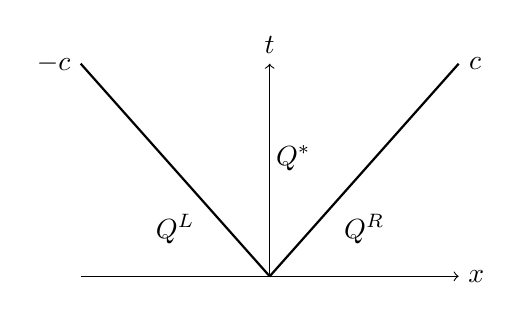
\begin{tikzpicture}[scale=0.6]
  \draw[->] (-4,0) -- (4.,0) node[right] {$x$};
  \draw[->] (0,0) -- (0,4.5) node[above] {$t$};
  \draw[thick] (0,0) -- (4.,4.5) node [right] {$c$};
  \draw[thick] (0,0) -- (-4.,4.5) node [left] {$-c$};
  \node at (2.,1.) {$\vect{Q}^R$};
  \node at (-2.,1.) {$\vect{Q}^L$};
  \node at (0.5,2.5) {$\vect{Q}^*$};
\end{tikzpicture}



%%% Local Variables:
%%% mode: latex
%%% TeX-master: "../../mainManuscript"
%%% End:

  \caption{Solution to Riemann problem \eqref{eq:Riemann_problem} for an elastic bar.}
  \label{fig:elasticity_example}
\end{figure}
Integration of characteristic equations \eqref{eq:elast_charac_equation} respectively along $AP$ and $BP$ yields:
\begin{equation}
  \label{eq:elastic_integral_curves}
  \left\lbrace
    \begin{aligned}
      -& \rho c \(v_P - v_A \) - \(\sigma_P - \sigma_A \) = 0\\
      & \rho c \(v_P - v_B \) - \(\sigma_P - \sigma_B \) = 0
    \end{aligned}
    \right.
\end{equation}
which solution is:
\begin{equation}
  \label{eq:elastic_solution_P}
  v_P = \frac{\sigma_B - \sigma_A}{2\rho c} + \frac{v_A+v_B}{2} \quad ; \quad \sigma_P = \rho c\frac{v_B - v_A}{2} + \frac{\sigma_A+\sigma_B}{2}
\end{equation}
On the other hand, the same procedure for point $P'$ leads to the solution:
\begin{equation}
  \label{eq:elastic_solution_Q}
  v_{P'} = \frac{\sigma_B - \sigma_{A'}}{2\rho c} + \frac{v_{A'}+v_B}{2} \quad ; \quad \sigma_{P'} = \rho c\frac{v_B - v_{A'}}{2} + \frac{\sigma_{A'}+\sigma_B}{2}
\end{equation}
With initial data given for the Riemann problem, it appears that $\Qcb_{A'}=\Qcb_{B}$ and hence, $\Qcb_{P'}=\Qcb_{R} \ne \Qcb_{P}$. Let's assume now that points $P$ and $P'$ are still on each side of the right characteristic straight line emanating from the origin but infinitely close to it. It is obvious that the previous results hold and that the a jump discontinuity propagates in the bar with speed $c$. Hence, we are left with the following condition across a discontinuous wave \cite{Toro} that generalizes to all linear Riemann problems:
\begin{definition}
Given a system of hyperbolic conservation laws $\Qcb_t + \Fcb(\Qcb)_x=\vect{0}$ and a discontinuous wave solution of speed $s_i$ associated to the $i$th characteristic field, the \textbf{Rankine-Hugoniot condition} reads:
\begin{equation}
  \label{eq:rankine-hugoniot}
  \saut{ \Fcb} = s_i \saut{ \Qcb}
\end{equation}
where $\saut{\bullet}$ denotes the jump operator across the discontinuity.  
\end{definition}

\subsubsection*{Characteristic variables -- Waves solution}
Consider a quasi-linear form of dimension $m$ $\Qcb_t + \Jbsf \Qcb_x=\vect{0}$. 
By introducing a set of \textbf{characteristic variables} $\Pcb=\Rbsf^{-1}\Qcb$, where $\Rsf_{ij}=\Rc^j_i$ is the matrix of right eigenvectors, the quasi-linear form of system \eqref{eq:Riemann_problem} can be rewritten in terms of characteristic the variables:
\begin{equation*}
  \begin{aligned}
    &\drond{\Pc_i}{t} + c_i\drond{\Pc_i}{x} = 0 \\
    &\left\lbrace 
      \begin{aligned}
        & \Pc_i(x,t=0) = \Pc_i^L \quad \text{if } x< 0\\
        & \Pc_i(x,t=0) = \Pc_i^R \quad \text{if } x> 0
      \end{aligned}
    \right.
  \end{aligned}
\end{equation*}
with $\Csf_{ij}=c_i\delta_{ij}$, the matrix of eigenvalues so that $\Jsf_{ij} \Rc^j_k = \Rc^k_i\Csf_{kj}$. The solution of this problem is straightforward since it corresponds to a superposition of scalar linear advection equations namely, the initial profil $\Pc_i(x,t=0)$ simply propagates with speed $c_i$ as depicted in figure \ref{fig:advection}. Thus, at a given point $(x,t)$, the solution $\Pc_i(x,t)$ is simply given by tracing backward the characteristic of slope $c_i$ passing through this point to the $x$-axis, that is: $\Pc_i(x,t)=\Pc_i(x-c_it,0)$. 
\begin{figure}[h]
  \centering
  \subfloat{\begin{tikzpicture}[scale=0.75]
  \draw[->] (-4,0) -- (4.,0) node[right] {$x$};
  \draw[->] (0,0) -- (0,4.5) node[above] {$t$};
  \draw[thick] (0,0) -- (4.,4) node [right] {$c_i$};
  % \fill[black] (1.,3.) circle (0.05) node [above] {$P$};
  % \fill[black] (2.10,1.762499) circle (0.05) node [right] {$P'$};
  \draw[dotted] (-4,1.)-- (0,1) node [above left] {$t_1$} --(4.,1);
  \draw[dotted] (-4,2.)-- (0,2) node [above left] {$t_2$} --(4.,2);
  \node[above left] at (0,0) {$t_0$};
\end{tikzpicture}

%%% Local Variables:
%%% mode: latex
%%% TeX-master: "../../mainManuscript"
%%% End:}
  \subfloat{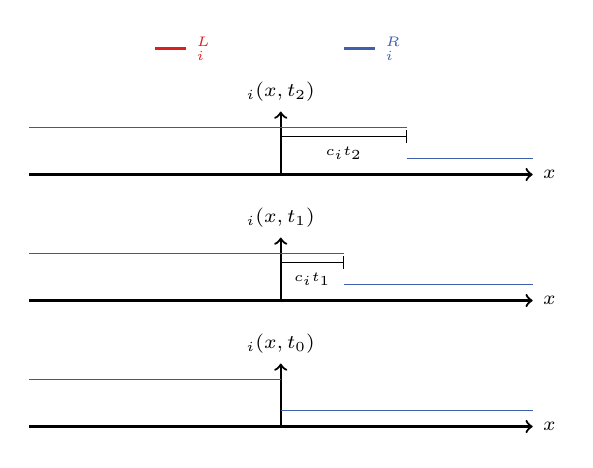
\begin{tikzpicture}[scale=0.8]
  %% t2
  \draw[->,thick] (0,0) -- (0,1) node [above] {\scriptsize$\Pc_i(x,t_2)$};
  \draw[->,thick] (-4,0) -- (4,0) node [right] {\scriptsize$x$};
  \draw[Blue] (2,0.25) -- (4,0.25);
  \draw[Red] (-4,0.75) -- (2,0.75);
  \draw (0,0.6)--(2,0.6) node [midway, below] {\tiny $c_it_2$};
  \draw (2,0.5)--(2,0.7);
  %% t1
  \draw[->,thick] (0,-2) -- (0,-1) node [above] {\scriptsize$\Pc_i(x,t_1)$};
  \draw[->,thick] (-4,-2) -- (4,-2) node [right] {\scriptsize$x$};
  \draw[Blue] (1,0.25-2) -- (4,0.25-2);
  \draw[Red] (-4,0.75-2) -- (1,0.75-2);
  \draw (0,0.6-2)--(1,0.6-2) node [midway, below] {\tiny $c_it_1$};
  \draw (1,0.5-2)--(1,0.7-2);
  %% t0
  \draw[->,thick] (0,-4) -- (0,-3) node [above] {\scriptsize$\Pc_i(x,t_0)$};
  \draw[->,thick] (-4,-4) -- (4,-4) node [right] {\scriptsize$x$};
  \draw[Blue] (0,0.25-4.) -- (4,0.25-4.);
  \draw[Red] (-4,0.75-4.) -- (0,0.75-4.);
  %% legend
  \draw[thick,Red] (-2.,2.) -- (-1.5,2.) node [right] {\scriptsize$\Pc_i^L$};
  \draw[thick,Blue] (1,2.) -- (1.5,2.) node [right] {\scriptsize$\Pc_i^R$};
\end{tikzpicture}
%%% Local Variables:
%%% mode: latex
%%% TeX-master: "../../mainManuscript"
%%% End:}
  \caption{Solution to linear advection equation on the quantity $\Pc_i$ with characteristic speed $c_i$.}
  \label{fig:advection}
\end{figure}
The vector $\Qcb$ is then determined by inverting the relation:
\begin{equation}
  \Qcb = \Rcb^i \Pc_i(x-c_it,0)
\end{equation}
or in terms of the initial data:
\begin{equation}
  \label{eq:Q_expansion}
  \Qcb = \sum_{i=1}^I \Rcb^i \Pc_i^R + \sum_{i=I+1}^m \Rcb^i \Pc_i^L
\end{equation}
where $m$ is $I$ is such that $x-c_I t >0$ and $x-c_{I+1} t <0$. This equation can be seen as an eigenvector expansion of $\Qcb$ with coefficients $\Pc_i^{R,L}$ and in particular:
\begin{equation}
  \label{eq:Qside_expansion}
  \Qcb^L = \sum_{i=1}^{m}\Rcb^i \Pc_i^L \quad ; \quad \Qcb^R = \sum_{i=1}^{m}\Rcb^i \Pc_i^R
\end{equation}
\begin{remark}
  The above discussion highlight the wave nature of the solution to hyperbolic problems. Indeed, since $\Qcb(x,t)$ can be expended into an eigenvector basis with coefficients $\Pc_i$ obeying a linear advection... 
\end{remark}
By rewritting expansion \eqref{eq:Q_expansion}:
\begin{align}
  &\Qcb = \sum_{i=1}^m \Rcb^i \Pc_i^R - \sum_{i=I+1}^m \Rcb^i \(\Pc_i^R - \Pc_i^L\)= \Qcb^R - \sum_{i=I+1}^m \Rcb^i \(\Pc_i^R - \Pc_i^L\) \\
  &\Qcb= \sum_{i=1}^{m}\Rcb^i \Pc_i^L + \sum_{i=1}^I \Rcb^i \(\Pc_i^R - \Pc_i^L\)= \Qcb^L + \sum_{i=1}^I \Rcb^i \(\Pc_i^R - \Pc_i^L\) 
\end{align}
Jump conditions can thus be derived:
\begin{align}
  \label{eq:jump_star_R}
  &  \Qcb-\Qcb^R = -\sum_{i=I+1}^{m} \Rcb^i\delta^i \\
  \label{eq:jump_star_L}
  &  \Qcb-\Qcb^L = \sum_{i=1}^{I} \Rcb^i\delta^i \\
\end{align}
where $\Qcb(x,t)$ is the state lying in the region of the ($x,t$) plane delimited by the $I$th and $(I+1)$th characteristics. In equations \eqref{eq:jump_star_R} and \eqref{eq:jump_star_L}, coefficients $\delta^i=\Pc_i^R - \Pc_i^L$ are called the \textit{wave strengths} and can be computed from \eqref{eq:Qside_expansion} by solving $\Qcb^R-\Qcb^L=\sum_{i=1}^{m}\Rcb^i \delta^i=\Rbsf \vect{\delta}$.

For the linear elastic case considered above, the wave strengths coeeficients are:
\begin{equation}
  \label{eq:elastic_wave_strengths}
  \vect{\delta} = \matrice{\frac{\rho c \(v_B - v_A\) + \(\sigma_B-\sigma_A\)}{2\rho c} \\\frac{\rho c \(v_B - v_A\) - \(\sigma_B-\sigma_A\)}{2\rho c}}
\end{equation}
leading, with equation \eqref{eq:jump_star_L} to:
\begin{equation}
  \label{eq:solution_charac_variables}
  \Qcb = \Qcb^L +\Rcb^1 \delta^1 = \matrice{\frac{\sigma_B - \sigma_A}{2\rho c} + \frac{v_A+v_B}{2} \\ \rho c\frac{v_B - v_A}{2} + \frac{\sigma_A+\sigma_B}{2}} 
\end{equation}
which is the solution found by using the method of characteristics \eqref{eq:elastic_solution_P}.
\subsection{Non-linear problems}
We now consider a hyperelastic medium made of a Saint-Venant-Kirchhoff material, infinite in directions $\vect{e}_2$ and $\vect{e}_3$, and semi-infinite in direction $\vect{e}_1$ (\textit{i.e. $x_1 \in [0,+\infty[$}). This medium suddenly undergoes a load at $(X_1=X=0,t=0)$ in direction $\vect{e}_1$ so that the deformation gradient and the PK1 tensor are respectively:
\begin{align*}
  &\tens{F}=F\vect{e}_1\otimes\vect{e}_1 + \vect{e}_2\otimes\vect{e}_2 + \vect{e}_3\otimes\vect{e}_3 \\
  & \tens{\Pi}=\Pi_{11}\vect{e}_1\otimes\vect{e}_1 + \Pi_{22}\(\vect{e}_2\otimes\vect{e}_2 + \vect{e}_3\otimes\vect{e}_3 \)
\end{align*}
which corresponds to a plane wave solution. We assume that $F(0,t)=\bar{F}$ is given, leading to a \textit{Picard problem} involving both initial and boundary conditions with neglected body forces:
\begin{equation}
  \label{eq:Picard_problem}
  \begin{aligned}
  &\Qcb_t + \drond{\Fcb\cdot \vect{X}}{X_N} = \vect{0}, \\
  &\left\lbrace 
    \begin{aligned}
      & \Qcb(X_N,t=0) = \Qcb^R \quad \text{if } X_N> 0 \\
      & F(0,t) = \bar{F} 
    \end{aligned}
    \right.
  \end{aligned}
\end{equation}
with $\vect{N}=\vect{e}_1$ and:
\begin{equation*}
 \Qcb = \matrice{v \\ F} \quad ; \quad \Fcb = \matrice{-\frac{1}{\rho_0}\Pi \\ -v}
\end{equation*}
where $\Pi=\Pi_{11}$. Since the tangent modulus and the acoustic tensor of Saint-Venant-Kirchhoff model \eqref{eq:SVK_tangent},\eqref{eq:SVK_acoustic} depend on the deformation gradient, the quasi-linear form: $\Qcb_t + \drond{\Fcb}{\Qcb}\drond{\Qcb}{X}=\vect{0}$ is more convenient. The Jacobian matrix is then:
\begin{equation}
  \label{eq:quasi_SVK}
  \Jbsf=\drond{\Fcb}{\Qcb}=-\matrice{0 & -\frac{H_{1111}}{\rho_0} \\ 1 & 0}
\end{equation}
which leads to the characteristic fields:
\begin{equation}
  \label{eq:SVK_charac_fields}
  \left\lbrace
    \begin{aligned}
      & c_1=- \sqrt{\frac{\lambda+2\mu}{2\rho_0}\(3F^2-1\) }\\
      &c_2= \sqrt{\frac{\lambda+2\mu}{2\rho_0}\(3F^2-1\) }
    \end{aligned}\right.
 \quad ; \quad \Lcb^p=\[1\:,\:- c_p \] \quad ; \quad \Rcb^p=\matrice{- c_p \\1} 
\end{equation}
Note that the non-linear flux function (\textit{i.e.} $\ddrond{\Pi_{11}}{F}{F}\neq 0$) yields characteristic fields depending on the strain state and, for the Saint-Venant--Kirchhoff model, possibly complex celerities leading to a loss of hyperbolicity of the problem for $F>\sqrt{\frac{1}{3}}$.

Initial and boundary conditions have an influence on the characteristic structure of the solution due to the dependence of characteristic speeds on the deformation gradient. Indeed, if initial data are given so that $\bar{F} > F_R$, the resulting characteristic speeds satisfy $c_2(\bar{F})>c_2(F_R)$ leading to characteristics colliding in the right region of the ($x,t$) plane (figure \ref{fig:Picard_problem}\subref{subfig:2S}). On the other hand, $\bar{F} < F_R$ yields characteristic moving away from each other in the right region according to $c_2(\bar{F})<c_2(F_R)$ (figure \ref{fig:Picard_problem}\subref{subfig:2R}). Those two situations, respectively corresponding to a shock wave and a simple wave, will be studied in what follows.
\begin{figure}[h]
  \centering
  \subfloat[Right-going shock wave\label{subfig:2S}]{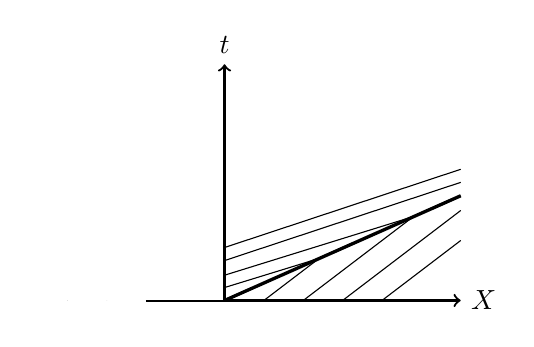
\begin{tikzpicture}
  \draw[->,thick] (-1,0) -- (3,0) node[right] {$X$};
  \draw[->,thick](0,0) -- (0,3) node[above] {$t$};
  \draw(-0.5,0.01) -- (1.20,0.533333) ;
  \draw(-1,0.01) -- (2.40,1.066) ;
  \draw(-1.5,0.01) -- (3,1.5) ;
  \draw(-2,0.01) -- (3,1.666) ;
  %%%%%%%%% 
  \draw(0.5,0) -- (1.20,0.533333) ;
  \draw(1.,0) -- (2.40,1.066) ;
  \draw(1.5,0) -- (3,1.14285) ;
  \draw(2.0,0) -- (3,0.7619) ;
  \draw[very thick] (0,0) -- (3,1.33);
  \fill[white] (-2.5,2.5) rectangle (-0.015,0.01);
  \fill[white] (-2.,0) rectangle (-1.,0.1);
\end{tikzpicture}}
  \subfloat[Right-going simple wave\label{subfig:2R}]{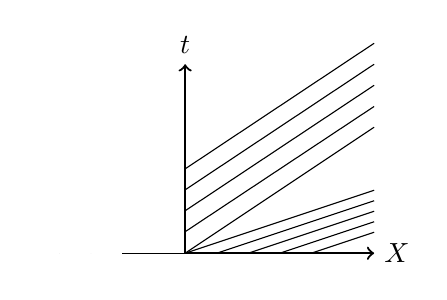
\begin{tikzpicture}[scale=0.8]
  \draw[->,thick] (-1,0) -- (3,0) node[right] {$X$};
  \draw[->,thick](0,0) -- (0,3) node[above] {$t$};
  \draw(0,0) -- (3,2) ;
  \draw(-0.5,0.01) -- (3,2.33) ;
  \draw(-1,0.01) -- (3,2.666) ;
  \draw(-1.5,0.01) -- (3,3) ;
  \draw(-2,0.01) -- (3,3.333) ;
  \draw(0,0) -- (3,1) ;
  \draw(0.5,0) -- (3,0.833) ;
  \draw(1,0) -- (3,0.666) ;
  \draw(1.5,0) -- (3,0.5) ;
  \draw(2,0) -- (3,0.333);
  \fill[white] (-2.5,2.5) rectangle (-0.015,0.01);
  \fill[white] (-2.,0) rectangle (-1.,0.1);
\end{tikzpicture}}
  \caption{Solutions to Picard problem \eqref{eq:Picard_problem} depending on initial and boundary data.}
  \label{fig:Picard_problem}
\end{figure}

\subsubsection*{Shock waves}
By applying the method of characteristics between the $x$-axis and an intersection point of two characteristic straight lines allows to show that a shock wave carry a jump discontinuity of the conserved quantity vector and hence, satisfy the Rankine-Hugoniot condition \eqref{eq:rankine-hugoniot} where the shock speed $s_i$ is to be defined. According to Rankine-Hugoniot conditions, those states obey:
\begin{align}
  \label{eq:RH_velocity}
  & -\frac{1}{\rho_0}\(\bar{\Pi} - \Pi_R \) = s \( \bar{v} - v_R \)\\
  \label{eq:RH_F}
  & - \( \bar{v}-v_R\)=s\( \bar{F} - F_R\)
\end{align}
For the sake of generality, $\bar{F}$ is considered as an unknown so that a relation connecting $\Qcb^R$ to a set of solutions $\Qcb$ through a shock wave can be developed.

Substitution of $s$ from equation \eqref{eq:RH_F} and introduction in equation \eqref{eq:RH_velocity} where $\Pi=\frac{\lambda+2\mu}{2}\(F^3-F\)$ yield:
\begin{align}
  \label{eq:shock_speed}
  & s=-\frac{v-v_R}{F - F_R}\\
  \label{eq:v_jump}
  & v-v_R= \pm \sqrt{\frac{\lambda+2\mu}{2\rho_0}(F-F_R)\[ F^3-F - (F_R^3-F_R)\]}
\end{align}
In addition to the Rankine-Hugoniot condition, the \textit{Lax entropy condition} stating that characteristic curves collide in a shock wave must be satisfied \cite[p.268]{Leveque}:
\begin{equation}
  \label{eq:Lax_entropy}
  \lambda(F)<s<\lambda(F_R)
\end{equation}
For a Saint-Venant--Kirchhoff material, the Lax condition leads to $F > F_R$ ensuring thus that the square root in equation \eqref{eq:v_jump} is real.


Equation \eqref{eq:v_jump} yields two families of curves in the phase plane, one of which is expected to identify with the jump conditions derived for the linear case \eqref{eq:jump_star_R} when considering an infinitesimal jump (\textit{i.e. $F=F_R+\epsilon$ with $\epsilon \rightarrow 0$}). Thus, equation \eqref{eq:v_jump} reads:
\begin{equation}
  \label{eq:linearization}
  v-v_R= \pm \sqrt{\frac{\lambda+2\mu}{2\rho_0}\epsilon\[ (F_R+\epsilon)^3-(F_R+\epsilon) - (F_R^3-F_R)\]}
\end{equation}
where, with $\epsilon \rightarrow 0$:
\begin{equation*}
  (F_R+\epsilon)^3\approx F_R^3(1+\frac{3\epsilon}{F_R})
\end{equation*}
and hence,
\begin{equation*}
  \matrice{v \\ F}=\matrice{v_R \\ F_R} + \epsilon \matrice{1 \\\pm \sqrt{\frac{\lambda+2\mu}{2\rho_0}\[ 3F_R^2-1\]}}
\end{equation*}
Hence, the \textit{minus} sign yields the linearized expression \eqref{eq:jump_star_R} for a right-going shock, the \textit{plus} sign holds, on the other hand, for left-going shocks. Finally, the Rankine-Hugoniot condition across a left-going shock and a right-going shock respectively yields:
\begin{align}
  \label{eq:left-going_shock}
  &v-v_L= \sqrt{\frac{\lambda+2\mu}{2\rho_0}(F-F_L)\[ F^3-F - (F_L^3-F_L)\]} \\
  \label{eq:right-going_shock}
  &v-v_R= -\sqrt{\frac{\lambda+2\mu}{2\rho_0}(F-F_R)\[ F^3-F - (F_R^3-F_R)\]}
\end{align}

\subsubsection*{Simple waves}
In order to study the evolution of fields within the void region in figure \ref{fig:Picard_problem}\subref{subfig:2R}, let's write the left-going characteristic equation through it with $\Lcb^1=[1,-c_1]$:
\begin{equation}
  \label{eq:SVK_rarefaction}
  dv -c_1  dF = 0 %+\sqrt{\frac{\lambda + 2\mu}{2\rho_0}\(3F^2-1\)}
\end{equation}

\begin{remark}
  If one was seeking a similarity solution in this region, the conserved quantity vector would be looked for so that $\Qcb'(x/t)$ is proportional to the right eigenvector $\Rcb^2$ asrequired by equation \eqref{eq:quasi-linear_similarity}. By denoting the ray $\xi=x/t$, this proportionality condition is:
  \begin{equation*}
    \matrice{\ddroit{v}{\xi} \\ \ddroit{F}{\xi}} = \matrice{ -c_2 \\ 1}
  \end{equation*}
  Combining these equations and noting that $c_2=-c_1$ allows to recover equation \eqref{eq:SVK_rarefaction}:
  \begin{equation}
    \label{eq:rarefaction}
    \begin{aligned}
      & dv -c_1 d\xi = 0\\
      & dF = d\xi
    \end{aligned}
  \end{equation}
Hence, the structure depicted in figure \ref{fig:Picard_problem}\subref{subfig:2R} corresponds to a rarefaction wave. Fields evolve smoothly within the void region according to equations \eqref{eq:rarefaction}, leading to a characteristic fan since $c_2=c_2(F)$ and $F$ decreases from $F_R$ to $\bar{F}$.
\end{remark}


As for shock waves, the complete set of states $\Qcb$ connected to $\Qcb^R$ through a rarefaction wave will be derived. To do so, the following change of variable is introduced: $F \mapsto ch(x)/\sqrt{3}$, so that equation \eqref{eq:SVK_rarefaction} becomes:
\begin{equation}
  \label{eq:charac_equation_sh}
  dv=-\sqrt{\frac{\lambda + 2\mu}{6\rho_0}}sh(x)^2 dx
\end{equation}
where, the hyperbolic cosine $ch(x)$ and sine $sh(x)$ satisfy: $ch(x)^2-sh(x)^2=1$. Equation \eqref{eq:charac_equation_sh} can be easily integrated with the exponential form of hyperbolic sine: $sh(x)=\frac{e^x - e^{-x}}{2}$. Thus, one gets:
\begin{equation*}
  v-v_R=-\frac{1}{4}\sqrt{\frac{\lambda + 2\mu}{6\rho_0}}\[sh(2x)-2x -(sh(2x_R)-2x_R)\]
\end{equation*}
At last, the inverse change of variable:
\begin{align*}
  &sh(2x)=2ch(x)sh(x)=2\sqrt{3}F\sqrt{3F^2-1} \\
  &2x=2\arg\(ch(\sqrt{3}F)\)=2\ln\(\sqrt{3}F + \sqrt{3F^2-1}\)
\end{align*}
yields the relation:
\begin{equation}
  \label{eq:integral_curve_right}
  v-v_R=-\sqrt{\frac{\lambda + 2\mu}{24\rho_0}}\[\sqrt{3}\(F\sqrt{3F^2-1} -F_R\sqrt{3F_R^2-1}\)-\ln\(\frac{\sqrt{3}F + \sqrt{3F^2-1}}{\sqrt{3}F_R + \sqrt{3F_R^2-1}}\) \]
\end{equation}
In a similar manner, the following condition must hold through a left-going rarefaction wave:
\begin{equation*}
  dv -c_2  dF = 0
\end{equation*}
which leads to:
\begin{equation}
  \label{eq:integral_curve_left}
  v-v_L=\sqrt{\frac{\lambda + 2\mu}{24\rho_0}}\[\sqrt{3}\(F\sqrt{3F^2-1} -F_L\sqrt{3F_L^2-1}\)-\ln\(\frac{\sqrt{3}F + \sqrt{3F^2-1}}{\sqrt{3}F_L + \sqrt{3F_L^2-1}}\) \]
\end{equation}



\subsubsection*{Solution to the Riemann problem}
Now the solution to Picard's problems have been derived, the solution to the Riemann problem can be developed. Once again, the problem is formulated as:
\begin{equation}
  \begin{aligned}
    &\Qcb_t + \drond{\Fcb\cdot \vect{N}}{X_N} = \vect{0}, \\
    &\left\lbrace 
      \begin{aligned}
        & \Qcb(X_N,t=0) = \Qcb^L \quad \text{if } X_N< 0\\
        & \Qcb(X_N,t=0) = \Qcb^R \quad \text{if } X_N> 0
      \end{aligned}
    \right.
  \end{aligned}
\end{equation}
As for the Picard problem, initial conditions influence the characteristic structure of the solution. Indeed, if initial conditions are given such that $F_L<F_R$, left-going characteristics will collide while right-going ones will move away from one another (see figure \ref{fig:RP_solution}\subref{subfig:1S2R}). In that case, the first and second characteristic fields will respectively be refered to as a \textit{1-shock} and a \textit{2-rarefaction}. Conversely, if $F_L>F_R$, the solution will correspond to a \textit{1-rarefaction} and a \textit{2-shock} (figure \ref{fig:RP_solution}\subref{subfig:1R2S}). 

\begin{figure}[h]
  \centering
  \subfloat[$F_L < F_R$\label{subfig:1S2R}]{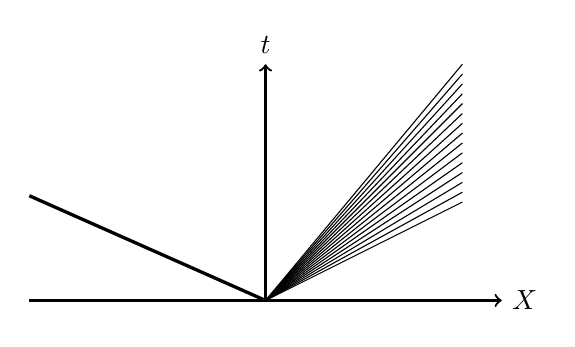
\begin{tikzpicture}
  \draw[->,thick] (-3,0) -- (3,0) node[right] {$X$};
  \draw[->,thick](0,0) -- (0,3) node[above] {$t$};
  %% Shock wave
  \draw[very thick] (0,0) -- (-3,1.33);
  %% Rarefaction wave
  \foreach \x in {0.5,0.55,...,1.25}
  \draw(0,0) -- (2.5,2.5*\x) ;
\end{tikzpicture}}
  \subfloat[$F_L > F_R$\label{subfig:1R2S}]{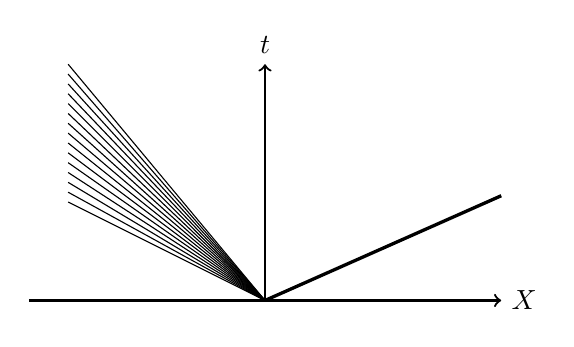
\begin{tikzpicture}
  \draw[->,thick] (-3,0) -- (3,0) node[right] {$X$};
  \draw[->,thick](0,0) -- (0,3) node[above] {$t$};
  %% Shock wave
  \draw[very thick] (0,0) -- (3,1.33);
  %% Rarefaction wave
  \foreach \x in {0.5,0.55,...,1.25}
  \draw(0,0) -- (-2.5,2.5*\x) ;
\end{tikzpicture}}
  \caption{General wave patterns arrising in the solution to Riemann problem depending on intial data. (a): 1-shock, 2-rarefaction. (b): 1-rarefaction, 2-shock.}
  \label{fig:RP_solution}
\end{figure}

For the 1-shock,2-rarefaction solution one then seeks a state $\Qcb^*$ that is connected to $\Qcb^L$ and $\Qcb^R$ through respectively a shock wave and a rarefaction wave. Hence, $\Qcb^*$ must satisfy equations \eqref{eq:left-going_shock} and \eqref{eq:integral_curve_right}, namely:
\begin{equation}
  \label{eq:1S2R_solution}
  \left\lbrace
  \begin{aligned}
    &v_*-v_L= \sqrt{\frac{\lambda+2\mu}{2\rho_0}(F_*-F_L)\[ F_*^3-F_* - (F_L^3-F_L)\]} \\
    &v_*-v_R=-\sqrt{\frac{\lambda + 2\mu}{24\rho_0}}\[\sqrt{3}\(F_*\sqrt{3F_*^2-1} -F_R\sqrt{3F_R^2-1}\)-\ln\(\frac{\sqrt{3}F_* + \sqrt{3F_*^2-1}}{\sqrt{3}F_R + \sqrt{3F_R^2-1}}\) \]
  \end{aligned}
  \right.
\end{equation}
Analogously, the 1-rarefaction,2-shock solution is given by the solution of equations \eqref{eq:integral_curve_left} and \eqref{eq:right-going_shock}:
\begin{equation}
  \label{eq:1R2S_solution}
  \left\lbrace
  \begin{aligned}
    &v_*-v_L=\sqrt{\frac{\lambda + 2\mu}{24\rho_0}}\[\sqrt{3}\(F_*\sqrt{3F_*^2-1} -F_L\sqrt{3F_L^2-1}\)-\ln\(\frac{\sqrt{3}F_* + \sqrt{3F_*^2-1}}{\sqrt{3}F_L + \sqrt{3F_L^2-1}}\) \]\\
    &v_*-v_R= -\sqrt{\frac{\lambda+2\mu}{2\rho_0}(F_*-F_R)\[ F_*^3-F_* - (F_R^3-F_R)\]}
  \end{aligned}
  \right.
\end{equation}
Once one of this system is solved, the solution $\Qcb$ is known everywhere except inside the rarefaction fan. Nevertheless, in this region $\Qcb$ only varies with the ray $\xi=c_i(F)$ and hence, the solution inside an $i$-rarefaction wave satisfies:
\begin{equation}
  \label{eq:rarefaction_fan}
  \xi = \pm \sqrt{\frac{\lambda + 2\mu}{2\rho_0}\(3F^2-1 \)} \quad \Rightarrow \quad F(\xi)= \sqrt{\frac{2\rho_0}{3(\lambda + 2\mu)}\xi^2-1}
\end{equation}
\begin{figure}[h]
  \centering
  \subfloat[Initial data: $F_L=1 ; F_R=2$ \label{subfig:1S2R_curves}]{\definecolor{Purple}{RGB}{120,28,129}
\definecolor{Blue}{RGB}{63,96,174}
\definecolor{Duck}{RGB}{83,158,182}
\definecolor{Green}{RGB}{109,179,136}
\definecolor{Yellow}{RGB}{202,184,67}
\definecolor{Orange}{RGB}{231,133,50}
\definecolor{Red}{RGB}{217,33,32}
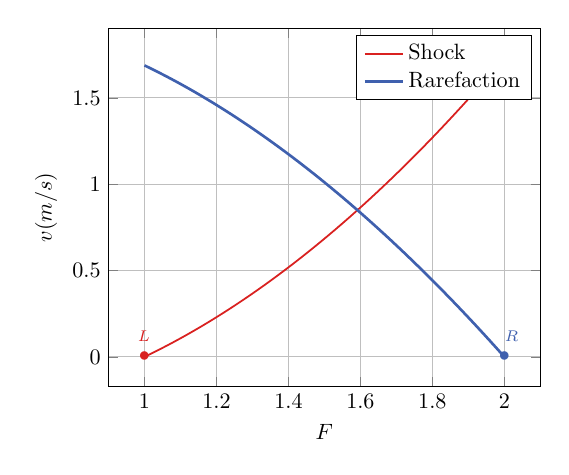
\begin{tikzpicture}[scale=0.8]
\begin{axis}[xlabel=$F$,ylabel=$v (m/s)$,ymajorgrids=true,xmajorgrids=true]
  \addplot[Red,thick] coordinates {(1.0,0.0) (1.0196019601960196,0.019889905868838792) (1.0392039203920391,0.04035480171519238) (1.058805880588059,0.06139339246981025) (1.0784078407840785,0.08300445472552491) (1.098009800980098,0.1051868317293367) (1.1176117611761176,0.1279394287977403) (1.1372137213721372,0.1512612091133456) (1.1568156815681567,0.17515118986560513) (1.1764176417641765,0.19960843870261852) (1.196019601960196,0.2246320704646163) (1.2156215621562156,0.25022124417291264) (1.2352235223522352,0.2763751602509047) (1.2548254825482548,0.30309305795616337) (1.2744274427442743,0.330374213004825) (1.2940294029402941,0.3582179353714115) (1.3136313631363137,0.386623567248899) (1.3332333233323332,0.4155904811553686) (1.3528352835283528,0.445118078174895) (1.3724372437243724,0.47520578632153143) (1.3920392039203922,0.5058530590163028) (1.4116411641164117,0.5370593736680643) (1.4312431243124313,0.568824230349938) (1.4508450845084508,0.6011471505637854) (1.4704470447044704,0.6340276760858663) (1.4900490049004902,0.667465367887438) (1.5096509650965095,0.7014598051246006) (1.5292529252925293,0.7360105841921958) (1.5488548854885489,0.7711173178369951) (1.5684568456845684,0.8067796343258441) (1.5880588058805882,0.8429971766647708) (1.6076607660766076,0.8797696018654025) (1.6272627262726274,0.917096580255355) (1.646864686468647,0.9549777948294852) (1.6664666466646665,0.9934129406392047) (1.686068606860686,1.032401724217221) (1.7056705670567056,1.0719438630353144) (1.7252725272527254,1.1120390849929296) (1.7448744874487447,1.1526871279345328) (1.7644764476447645,1.1938877391938512) (1.784078407840784,1.2356406751632294) (1.8036803680368036,1.2779457008865038) (1.8232823282328234,1.320802589673878) (1.8428842884288428,1.3642111227374165) (1.8624862486248626,1.4081710888458763) (1.8820882088208821,1.4526822839976499) (1.9016901690169017,1.4977445111107466) (1.9212921292129215,1.543357579728744) (1.9408940894089408,1.5895213057417645) (1.9604960496049606,1.6362355111215798) (1.9800980098009802,1.6835000236699957) (1.9996999699969997,1.7313146767797576) };
  \addplot[Blue,very thick] coordinates {(1.0,1.6884673989302577) (1.0196019601960196,1.6685781823289632) (1.0392039203920391,1.648117983645035) (1.058805880588059,1.6270917763366024) (1.0784078407840785,1.6055041425368688) (1.098009800980098,1.5833593157699348) (1.1176117611761176,1.5606612177002648) (1.1372137213721372,1.5374134899261505) (1.1568156815681567,1.5136195216278194) (1.1764176417641765,1.48928247372591) (1.196019601960196,1.4644053000848238) (1.2156215621562156,1.4389907661996928) (1.2352235223522352,1.4130414657294894) (1.2548254825482548,1.3865598351776642) (1.2744274427442743,1.3595481669723095) (1.2940294029402941,1.3320086211576845) (1.3136313631363137,1.3039432358761032) (1.3332333233323332,1.2753539367920979) (1.3528352835283528,1.246242545588463) (1.3724372437243724,1.216610787645106) (1.3920392039203922,1.1864602989961286) (1.4116411641164117,1.1557926326474621) (1.4312431243124313,1.12460926432638) (1.4508450845084508,1.092911597724879) (1.4704470447044704,1.0607009692909792) (1.4900490049004902,1.0279786526152188) (1.5096509650965095,0.994745862453826) (1.5292529252925293,0.9610037584250569) (1.5488548854885489,0.9267534484108921) (1.5684568456845684,0.8919959916925568) (1.5880588058805882,0.8567324018451127) (1.6076607660766076,0.8209636494135533) (1.6272627262726274,0.7846906643903794) (1.646864686468647,0.7479143385125069) (1.6664666466646665,0.7106355273934435) (1.686068606860686,0.6728550525050632) (1.7056705670567056,0.6345737030218022) (1.7252725272527254,0.595792237538853) (1.7448744874487447,0.5565113856747698) (1.7644764476447645,0.5167318495678894) (1.784078407840784,0.47645430527509447) (1.8036803680368036,0.43567940408061234) (1.8232823282328234,0.3944077737218566) (1.8428842884288428,0.3526400195386741) (1.8624862486248626,0.31037672555176576) (1.8820882088208821,0.2676184554755838) (1.9016901690169017,0.22436575367049583) (1.9212921292129215,0.18061914603862234) (1.9408940894089408,0.13637914086738703) (1.9604960496049606,0.09164622962443836) (1.9800980098009802,0.04642088770736517) (1.9996999699969997,0.0007035751512764867) };
  \node at (axis cs:1,0) [Red] {$\bullet$};
  \node at (axis cs:2.,0) [Blue] {$\bullet$};
  % \node[coordinate] at (axis cs:1.,0.) {$Mich$};
  \node at (axis cs:1,0) [anchor=south,Red] {$\Qcb^L$};
  \node at (axis cs:1.98,0) [above right,Blue] {$\Qcb^R$};
  \legend{Shock,Rarefaction}
  % \addplot[Blue,dashed,very thick,domain=1:2,samples=51,samples y=0]
  %   ({x},{0.-sqrt(0.5*(12.-1))*(x-2.)});
  % \addplot[Red,dashed,very thick,domain=1:2,samples=51,samples y=0]
  %   ({x},{0.+sqrt(0.5*(2.-1))*(x-1.)});
\end{axis}
\end{tikzpicture}
}
  \subfloat[Initial data: $F_L=2 ; F_R=1$ \label{subfig:1S2R_curves}]{\definecolor{Purple}{RGB}{120,28,129}
\definecolor{Blue}{RGB}{63,96,174}
\definecolor{Duck}{RGB}{83,158,182}
\definecolor{Green}{RGB}{109,179,136}
\definecolor{Yellow}{RGB}{202,184,67}
\definecolor{Orange}{RGB}{231,133,50}
\definecolor{Red}{RGB}{217,33,32}
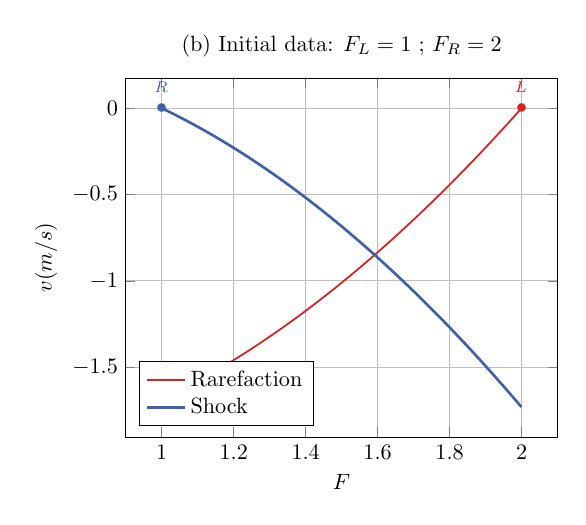
\begin{tikzpicture}[scale=0.8]
\begin{axis}[xlabel=$F$,ylabel=$v (m/s)$,ymajorgrids=true,xmajorgrids=true,legend pos=south west,title={(b) Initial data: $F_L=1$ ; $F_R=2$}]
  \addplot[Red,thick] coordinates {(1.0,-1.6884673989302577) (1.0196019601960196,-1.6685781823289632) (1.0392039203920391,-1.648117983645035) (1.058805880588059,-1.6270917763366024) (1.0784078407840785,-1.6055041425368688) (1.098009800980098,-1.5833593157699348) (1.1176117611761176,-1.5606612177002648) (1.1372137213721372,-1.5374134899261505) (1.1568156815681567,-1.5136195216278194) (1.1764176417641765,-1.48928247372591) (1.196019601960196,-1.4644053000848238) (1.2156215621562156,-1.4389907661996928) (1.2352235223522352,-1.4130414657294894) (1.2548254825482548,-1.3865598351776642) (1.2744274427442743,-1.3595481669723095) (1.2940294029402941,-1.3320086211576845) (1.3136313631363137,-1.3039432358761032) (1.3332333233323332,-1.2753539367920979) (1.3528352835283528,-1.246242545588463) (1.3724372437243724,-1.216610787645106) (1.3920392039203922,-1.1864602989961286) (1.4116411641164117,-1.1557926326474621) (1.4312431243124313,-1.12460926432638) (1.4508450845084508,-1.092911597724879) (1.4704470447044704,-1.0607009692909792) (1.4900490049004902,-1.0279786526152188) (1.5096509650965095,-0.994745862453826) (1.5292529252925293,-0.9610037584250569) (1.5488548854885489,-0.9267534484108921) (1.5684568456845684,-0.8919959916925568) (1.5880588058805882,-0.8567324018451127) (1.6076607660766076,-0.8209636494135533) (1.6272627262726274,-0.7846906643903794) (1.646864686468647,-0.7479143385125069) (1.6664666466646665,-0.7106355273934435) (1.686068606860686,-0.6728550525050632) (1.7056705670567056,-0.6345737030218022) (1.7252725272527254,-0.595792237538853) (1.7448744874487447,-0.5565113856747698) (1.7644764476447645,-0.5167318495678894) (1.784078407840784,-0.47645430527509447) (1.8036803680368036,-0.43567940408061234) (1.8232823282328234,-0.3944077737218566) (1.8428842884288428,-0.3526400195386741) (1.8624862486248626,-0.31037672555176576) (1.8820882088208821,-0.2676184554755838) (1.9016901690169017,-0.22436575367049583) (1.9212921292129215,-0.18061914603862234) (1.9408940894089408,-0.13637914086738703) (1.9604960496049606,-0.09164622962443836) (1.9800980098009802,-0.04642088770736517) (1.9996999699969997,-0.0007035751512764867) };
  \addplot[Blue,very thick] coordinates {(1.0,0.0) (1.0196019601960196,-0.019889905868838792) (1.0392039203920391,-0.04035480171519238) (1.058805880588059,-0.06139339246981025) (1.0784078407840785,-0.08300445472552491) (1.098009800980098,-0.1051868317293367) (1.1176117611761176,-0.1279394287977403) (1.1372137213721372,-0.1512612091133456) (1.1568156815681567,-0.17515118986560513) (1.1764176417641765,-0.19960843870261852) (1.196019601960196,-0.2246320704646163) (1.2156215621562156,-0.25022124417291264) (1.2352235223522352,-0.2763751602509047) (1.2548254825482548,-0.30309305795616337) (1.2744274427442743,-0.330374213004825) (1.2940294029402941,-0.3582179353714115) (1.3136313631363137,-0.386623567248899) (1.3332333233323332,-0.4155904811553686) (1.3528352835283528,-0.445118078174895) (1.3724372437243724,-0.47520578632153143) (1.3920392039203922,-0.5058530590163028) (1.4116411641164117,-0.5370593736680643) (1.4312431243124313,-0.568824230349938) (1.4508450845084508,-0.6011471505637854) (1.4704470447044704,-0.6340276760858663) (1.4900490049004902,-0.667465367887438) (1.5096509650965095,-0.7014598051246006) (1.5292529252925293,-0.7360105841921958) (1.5488548854885489,-0.7711173178369951) (1.5684568456845684,-0.8067796343258441) (1.5880588058805882,-0.8429971766647708) (1.6076607660766076,-0.8797696018654025) (1.6272627262726274,-0.917096580255355) (1.646864686468647,-0.9549777948294852) (1.6664666466646665,-0.9934129406392047) (1.686068606860686,-1.032401724217221) (1.7056705670567056,-1.0719438630353144) (1.7252725272527254,-1.1120390849929296) (1.7448744874487447,-1.1526871279345328) (1.7644764476447645,-1.1938877391938512) (1.784078407840784,-1.2356406751632294) (1.8036803680368036,-1.2779457008865038) (1.8232823282328234,-1.320802589673878) (1.8428842884288428,-1.3642111227374165) (1.8624862486248626,-1.4081710888458763) (1.8820882088208821,-1.4526822839976499) (1.9016901690169017,-1.4977445111107466) (1.9212921292129215,-1.543357579728744) (1.9408940894089408,-1.5895213057417645) (1.9604960496049606,-1.6362355111215798) (1.9800980098009802,-1.6835000236699957) (1.9996999699969997,-1.7313146767797576) };
  \node at (axis cs:1,0) [Blue] {$\bullet$};
  \node at (axis cs:2.,0) [Red] {$\bullet$};
  \node at (axis cs:1,0) [anchor=south,Blue] {$\Qcb^R$};
  \node at (axis cs:2,0) [anchor=south,Red] {$\Qcb^L$};
\legend{Rarefaction,Shock}
\end{axis}
\end{tikzpicture}
}
  \caption{Set of connected states $\Qcb$ to initial data through shock and rarefaction waves with $v_L=v_R=0$ in both cases: (a) 1-shock,2-rarefaction solution ; (b) 1-rarefaction, 2-shock.}
  \label{fig:solutions_RP}
\end{figure}


\begin{remark}
  The above discussion holds for concave flux functions which is not the case for the neo-Hookean model for instance. Indeed, such a model yields a monotonically decreasing positive characteristic speeds with the gradient of deformation (see figure \ref{fig:SVK-NH}\subref{subfig:SVK_NH_speeds}). Hence, initial data considered previously will lead to opposite situations (\textit{i.e. $F_L<F_R \rightarrow $ 1--rarefaction ; 2--shock, and $F_L>F_R \rightarrow $ 1--shock ; 2--rarefaction}). Moreover, the polyconvexity of the neo-Hookean stored energy function ensures the hyperbolicity of the system so that the problem does not suffer any limitation on the deformation gradient.
  \begin{figure}[h]
    \centering
    \subfloat[Stress $\Pi_{11}$ \label{subfig:SVK_NH_Pi}]{\definecolor{Red}{RGB}{217,33,32}
\definecolor{Blue}{RGB}{63,96,174}
\definecolor{Duck}{RGB}{83,158,182}
\definecolor{Green}{RGB}{109,179,136}
\definecolor{Yellow}{RGB}{202,184,67}
\definecolor{Orange}{RGB}{231,133,50}
\definecolor{Red}{RGB}{217,33,32}
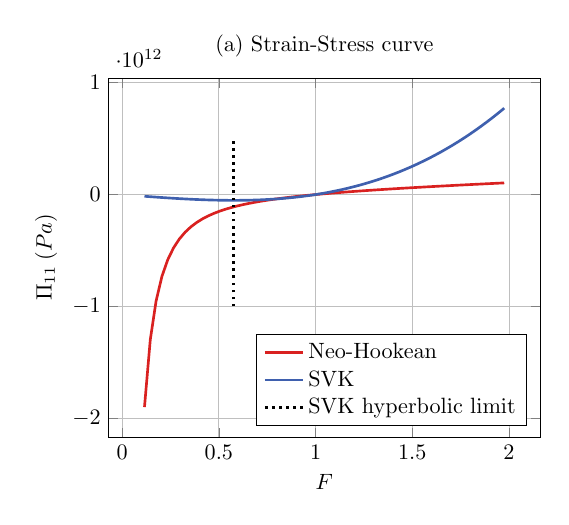
\begin{tikzpicture}[scale=0.8]
\begin{axis}[xlabel=$F$,ylabel=$\Pi_{11} \: (Pa)$,ymajorgrids=true,xmajorgrids=true,legend pos=south east,title={(a) Strain-Stress curve}]
\addplot[Red,very thick] coordinates {(0.11547005383792518,-1898966453319.162) (0.14547005383792516,-1296837707486.0405) (0.17547005383792513,-951312235719.5623) (0.20547005383792513,-732355105152.6451) (0.23547005383792513,-583575852118.2125) (0.2654700538379251,-477087968993.8754) (0.2954700538379251,-397729449724.4541) (0.3254700538379251,-336642141070.28204) (0.35547005383792507,-288349957545.72546) (0.38547005383792504,-249309520683.61847) (0.415470053837925,-217140040714.9308) (0.44547005383792504,-190190468824.5224) (0.475470053837925,-167284549773.97247) (0.505470053837925,-147564580724.34894) (0.535470053837925,-130392343185.27245) (0.5654700538379249,-115284401045.16144) (0.595470053837925,-101868733030.67676) (0.625470053837925,-89854990617.66492) (0.6554700538379249,-79013679521.07468) (0.6854700538379249,-69161318053.14328) (0.7154700538379248,-60149680216.69014) (0.7454700538379249,-51857881714.88495) (0.7754700538379249,-44186477584.150566) (0.8054700538379248,-37053004869.531456) (0.8354700538379248,-30388577783.986546) (0.8654700538379249,-24135259235.847366) (0.8954700538379248,-18244011798.887867) (0.9254700538379248,-12673085866.843775) (0.9554700538379248,-7386740998.494719) (0.9854700538379247,-2354223588.251995) (1.0154700538379247,2451056537.9352818) (1.0454700538379247,7052193879.264957) (1.0754700538379247,11469332294.041113) (1.1054700538379247,15720112571.176903) (1.1354700538379248,19820042073.450085) (1.1654700538379246,23782801671.8228) (1.1954700538379246,27620501912.14364) (1.2254700538379246,31343897846.142628) (1.2554700538379246,34962570023.63762) (1.2854700538379247,38485077640.53793) (1.3154700538379245,41919088663.206696) (1.3454700538379245,45271490826.59238) (1.3754700538379245,48548486673.378265) (1.4054700538379246,51755675220.64049) (1.4354700538379246,54898122376.10795) (1.4654700538379246,57980421852.87309) (1.4954700538379244,61006748029.95563) (1.5254700538379244,63980901961.52675) (1.5554700538379245,66906351538.24785) (1.5854700538379245,69786266641.0072) (1.6154700538379245,72623549993.23035) (1.6454700538379243,75420864307.28705) (1.6754700538379244,78180656228.87244) (1.7054700538379244,80905177507.05946) (1.7354700538379244,83596503754.174) (1.7654700538379244,86256551106.45828) (1.7954700538379245,88887091051.8295) (1.8254700538379243,91489763653.42323) (1.8554700538379243,94066089365.83081) (1.8854700538379243,96617479614.0105) (1.9154700538379243,99145246281.97147) (1.9454700538379244,101650610238.83322) (1.9754700538379242,104134709013.2085) };
\addplot[Blue,very thick] coordinates {(0.11547005383792518,-15336791766.165447) (0.14547005383792516,-19168111304.289738) (0.17547005383792513,-22893685303.277996) (0.20547005383792513,-26491706070.822536) (0.23547005383792513,-29940365914.61566) (0.2654700538379251,-33217857142.349674) (0.2954700538379251,-36302372061.71689) (0.3254700538379251,-39172102980.40962) (0.35547005383792507,-41805242206.12016) (0.38547005383792504,-44179982046.540825) (0.415470053837925,-46274514809.36392) (0.44547005383792504,-48067032802.28176) (0.475470053837925,-49535728332.98665) (0.505470053837925,-50658793709.17089) (0.535470053837925,-51414421238.526794) (0.5654700538379249,-51780803228.74666) (0.595470053837925,-51736131987.522804) (0.625470053837925,-51258599822.54755) (0.6554700538379249,-50326399041.513176) (0.6854700538379249,-48917721952.112) (0.7154700538379248,-47010760862.036354) (0.7454700538379249,-44583708078.97849) (0.7754700538379249,-41614755910.630775) (0.8054700538379248,-38082096664.68549) (0.8354700538379248,-33963922648.83495) (0.8654700538379249,-29238426170.77144) (0.8954700538379248,-23883799538.187305) (0.9254700538379248,-17878235058.774815) (0.9554700538379248,-11199925040.226295) (0.9854700538379247,-3827061790.2340784) (1.0154700538379247,4262162383.5095387) (1.0454700538379247,13089555173.312326) (1.0754700538379247,22676924271.481888) (1.1054700538379247,33046077370.32594) (1.1354700538379248,44218822162.15218) (1.1654700538379246,56216966339.268196) (1.1954700538379246,69062317593.98189) (1.2254700538379246,82776683618.60081) (1.2554700538379246,97381872105.43274) (1.2854700538379247,112899690746.78526) (1.3154700538379245,129351947234.96603) (1.3454700538379245,146760449262.28293) (1.3754700538379245,165147004521.04358) (1.4054700538379246,184533420703.55563) (1.4354700538379246,204941505502.12674) (1.4654700538379246,226393066609.06476) (1.4954700538379244,248909911716.677) (1.5254700538379244,272513848517.2716) (1.5554700538379245,297226684703.1562) (1.5854700538379245,323070227966.6382) (1.6154700538379245,350066286000.0256) (1.6454700538379243,378236666495.6256) (1.6754700538379244,407603177145.7466) (1.7054700538379244,438187625642.6959) (1.7354700538379244,470011819678.7812) (1.7654700538379244,503097566946.3102) (1.7954700538379245,537466675137.5906) (1.8254700538379243,573140951944.9299) (1.8554700538379243,610142205060.6364) (1.8854700538379243,648492242177.0171) (1.9154700538379243,688212870986.3801) (1.9454700538379244,729325899181.0331) (1.9754700538379242,771853134453.2832) };
\addplot[dotted,very thick] coordinates {(sqrt(1./3.),-1.e12) (sqrt(1./3.),0.5e12)};
\legend{Neo-Hookean,SVK,SVK hyperbolic limit}
\end{axis}
\end{tikzpicture}
}
    \subfloat[Characteristic speeds\label{subfig:SVK_NH_speeds}]{\definecolor{Red}{RGB}{217,33,32}
\definecolor{Blue}{RGB}{63,96,174}
\definecolor{Duck}{RGB}{83,158,182}
\definecolor{Green}{RGB}{109,179,136}
\definecolor{Yellow}{RGB}{202,184,67}
\definecolor{Orange}{RGB}{231,133,50}
\definecolor{Red}{RGB}{217,33,32}
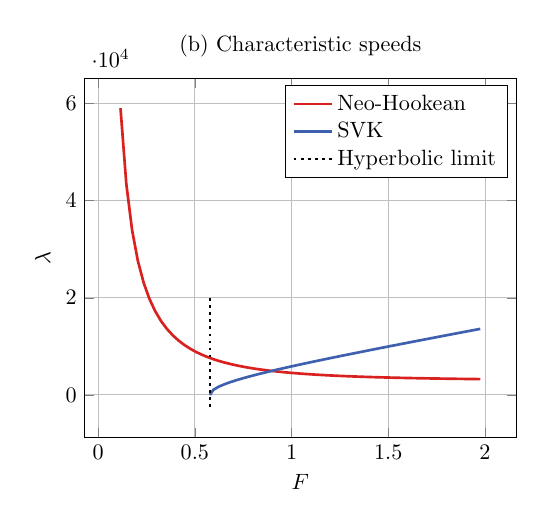
\begin{tikzpicture}[scale=0.8]
\begin{axis}[xlabel=$F$,ylabel=$\abs{\lambda}$,ymajorgrids=true,xmajorgrids=true,title={(b) Characteristic speeds}]
\addplot[Red,very thick] coordinates {(0.11547005383792518,59012.035730808406) (0.14547005383792516,43444.15680640866) (0.17547005383792513,33909.66271892359) (0.20547005383792513,27551.616086072518) (0.23547005383792513,23052.45426344622) (0.2654700538379251,19726.297080765253) (0.2954700538379251,17183.410876622853) (0.3254700538379251,15187.108927674422) (0.35547005383792507,13585.92851121213) (0.38547005383792504,12278.756336822797) (0.415470053837925,11195.691489974464) (0.44547005383792504,10286.970773511453) (0.475470053837925,9516.269220270638) (0.505470053837925,8856.492138358943) (0.535470053837925,8287.045413546242) (0.5654700538379249,7792.014425579814) (0.595470053837925,7358.918900548452) (0.625470053837925,6977.8428382999955) (0.6554700538379249,6640.81463208358) (0.6854700538379249,6341.3576871839605) (0.7154700538379248,6074.159484360366) (0.7454700538379249,5834.824367261866) (0.7754700538379249,5619.6864514897625) (0.8054700538379248,5425.666332338412) (0.8354700538379248,5250.16012367266) (0.8654700538379249,5090.952654625974) (0.8954700538379248,4946.148920983796) (0.9254700538379248,4814.119475233549) (0.9554700538379248,4693.456563660641) (0.9854700538379247,4582.938625301644) (1.0154700538379247,4481.501352586511) (1.0454700538379247,4388.21394243672) (1.0754700538379247,4302.259484218307) (1.1054700538379247,4222.918668359039) (1.1354700538379248,4149.556178447647) (1.1654700538379246,4081.609265724866) (1.1954700538379246,4018.57810915085) (1.2254700538379246,3960.0176447237714) (1.2554700538379246,3905.530610294456) (1.2854700538379247,3854.761601089376) (1.3154700538379245,3807.391969723345) (1.3454700538379245,3763.135435049281) (1.3754700538379245,3721.7342885593334) (1.4054700538379246,3682.9561065868374) (1.4354700538379246,3646.590892305437) (1.4654700538379246,3612.448584281259) (1.4954700538379244,3580.3568787248346) (1.5254700538379244,3550.1593210921387) (1.5554700538379245,3521.7136296737963) (1.5854700538379245,3494.8902195829423) (1.6154700538379245,3469.5709003379666) (1.6454700538379243,3445.6477242208375) (1.6754700538379244,3423.021965921998) (1.7054700538379244,3401.6032167766175) (1.7354700538379244,3381.308579249105) (1.7654700538379244,3362.061949309672) (1.7954700538379245,3343.793376030597) (1.8254700538379243,3326.438489161275) (1.8554700538379243,3309.9379866615427) (1.8854700538379243,3294.237175216221) (1.9154700538379243,3279.2855576483526) (1.9454700538379244,3265.0364619174256) (1.9754700538379242,3251.446707051308) };
\addplot[Blue,very thick] coordinates {(sqrt(1./3.),0.) (0.595470053837925,1048.9455179543422) (0.625470053837925,1731.1029259571128) (0.6554700538379249,2233.012146664284) (0.6854700538379249,2658.790029377158) (0.7154700538379248,3040.5889001561395) (0.7454700538379249,3393.286396027051) (0.7754700538379249,3725.1576526965905) (0.8054700538379248,4041.336632315833) (0.8354700538379248,4345.250197655363) (0.8654700538379249,4639.309436869055) (0.8954700538379248,4925.279696432755) (0.9254700538379248,5204.494537554574) (0.9554700538379248,5477.987035494905) (0.9854700538379247,5746.574266198714) (1.0154700538379247,6010.9138156437175) (1.0454700538379247,6271.542813975518) (1.0754700538379247,6528.905643538706) (1.1054700538379247,6783.374072186155) (1.1354700538379248,7035.262182069363) (1.1654700538379246,7284.837637447764) (1.1954700538379246,7532.330323596269) (1.2254700538379246,7777.939063134427) (1.2554700538379246,8021.836903239133) (1.2854700538379247,8264.175324905573) (1.3154700538379245,8505.087628335128) (1.3454700538379245,8744.691681060722) (1.3754700538379245,8983.092167747032) (1.4054700538379246,9220.382446402957) (1.4354700538379246,9456.646090866763) (1.4654700538379246,9691.958181097758) (1.4954700538379244,9926.386389147965) (1.5254700538379244,10159.991898394823) (1.5554700538379245,10392.830185782268) (1.5854700538379245,10624.951690800193) (1.6154700538379245,10856.402390269113) (1.6454700538379243,11087.224294354115) (1.6754700538379244,11317.455876364773) (1.7054700538379244,11547.132446624275) (1.7354700538379244,11776.286478876727) (1.7654700538379244,12004.947896244235) (1.7954700538379245,12233.144322567889) (1.8254700538379243,12460.901304010209) (1.8554700538379243,12688.242505014787) (1.8854700538379243,12915.189882077482) (1.9154700538379243,13141.763838254037) (1.9454700538379244,13367.983360890252) (1.9754700538379242,13593.866144695845) };
\addplot[dotted,very thick] coordinates {(sqrt(1./3.),-0.25e4) (sqrt(1./3.),2.e4)};
\legend{Neo-Hookean,SVK,Hyperbolic limit}
\end{axis}
\end{tikzpicture}
}
    \caption{Comparison of neo--Hookean and Saint-Venant--Kirchhoff hyperelastic models.}
    \label{fig:SVK-NH}
  \end{figure}
  At last, figure \ref{fig:SVK-NH}\subref{subfig:SVK_NH_Pi} highlights the non-physical behaviour of Saint-Venant-Kirchhoff model for high compression loads that lead to a stress tensor tending to zero.
\end{remark}


%%% Local Variables:
%%% mode: latex
%%% TeX-master: "../mainManuscript"
%%% End:



\section{Derivation of one-dimensional solid mechanics solutions}
\label{sec:analytical_results}
%\documentclass[crop,tikz]{standalone}
\usepackage{pgfplots}
\usetikzlibrary{pgfplots.groupplots}

\begin{document}
\definecolor{Purple}{RGB}{120,28,129}
\definecolor{Orange}{RGB}{231,133,50}
\definecolor{Blue}{RGB}{63,96,174}
\definecolor{Red}{RGB}{217,33,32}
\definecolor{Duck}{RGB}{83,158,182}
\definecolor{Green}{RGB}{109,179,136}
\definecolor{Yellow}{RGB}{202,184,67}
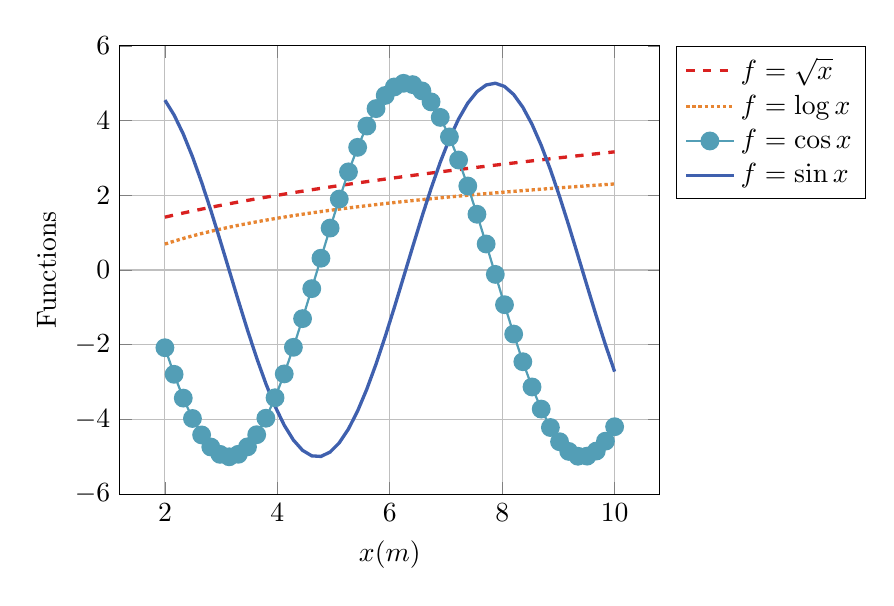
\begin{tikzpicture}[scale=1.]
\begin{axis}[xlabel=$x (m)$,ylabel=Functions,ymajorgrids=true,xmajorgrids=true,legend pos=outer north east,title={}]
\addplot[Red,very thick,mark=none,dashed,mark size=3pt] coordinates {(2.0,1.4142135623730951) (2.163265306122449,1.4708043058552858) (2.326530612244898,1.52529689314733) (2.489795918367347,1.5779087167410373) (2.6530612244897958,1.6288220358559113) (2.816326530612245,1.6781914463529615) (2.979591836734694,1.7261494247992246) (3.142857142857143,1.7728105208558367) (3.3061224489795915,1.8182745801939793) (3.4693877551020407,1.8626292586293283) (3.63265306122449,1.9059520091609048) (3.7959183673469385,1.9483116709979793) (3.9591836734693877,1.9897697538834456) (4.122448979591836,2.030381486221699) (4.285714285714286,2.0701966780270626) (4.448979591836734,2.1092604371762) (4.612244897959183,2.147613768338987) (4.775510204081632,2.1852940772540506) (4.938775510204081,2.2223355980148636) (5.1020408163265305,2.2587697572631282) (5.26530612244898,2.294625486315573) (5.428571428571429,2.32992949004287) (5.591836734693877,2.3647064796066926) (5.755102040816326,2.3989793748209522) (5.918367346938775,2.4327694808466287) (6.081632653061225,2.4660966430902955) (6.244897959183673,2.498979383505129) (6.408163265306122,2.531435020952764) (6.571428571428571,2.5634797778466227) (6.73469387755102,2.5951288749407073) (6.897959183673469,2.626396615835748) (7.061224489795918,2.657296462534039) (7.224489795918367,2.6878411031752543) (7.387755102040816,2.718042512920064) (7.551020408163265,2.747912008810192) (7.7142857142857135,2.7774602993176543) (7.877551020408163,2.806697529198357) (8.040816326530612,2.835633320182744) (8.204081632653061,2.864276807966203) (8.367346938775508,2.892636675902369) (8.53061224489796,2.920721185751553) (8.693877551020407,2.948538205792899) (8.857142857142858,2.9760952365713798) (9.020408163265305,3.0033994345183768) (9.183673469387754,3.0304576336566322) (9.346938775510203,3.0572763655760995) (9.510204081632653,3.083861877846129) (9.673469387755102,3.1102201510110343) (9.83673469387755,3.136356914300021) (10.0,3.1622776601683795) };
\addplot[Orange,very thick,mark=none,densely dotted,mark size=3pt] coordinates {(2.0,0.6931471805599453) (2.163265306122449,0.7716187960014406) (2.326530612244898,0.8443781502838689) (2.489795918367347,0.91220074662263) (2.6530612244897958,0.9757141523449557) (2.816326530612245,1.0354333870465782) (2.979591836734694,1.0917863235977099) (3.142857142857143,1.1451323043030026) (3.3061224489795915,1.1957760371217574) (3.4693877551020407,1.2439781389396352) (3.63265306122449,1.2899632521814586) (3.7959183673469385,1.3339263756025745) (3.9591836734693877,1.3760378609527015) (4.122448979591836,1.4164473992905782) (4.285714285714286,1.455287232606842) (4.448979591836734,1.4926747646784622) (4.612244897959183,1.528714701161659) (4.775510204081632,1.5635008172470748) (4.938775510204081,1.5971174280460598) (5.1020408163265305,1.6296406197516198) (5.26530612244898,1.6611392868109909) (5.428571428571429,1.6916760106710724) (5.591836734693877,1.7213078082774436) (5.755102040816326,1.750086772827487) (5.918367346938775,1.7780606248698931) (6.081632653061225,1.805273188394778) (6.244897959183673,1.831764803841754) (6.408163265306122,1.8575726877976266) (6.571428571428571,1.8827312474337816) (6.73469387755102,1.9072723563498992) (6.897959183673469,1.931225597372392) (7.061224489795918,1.9546184769470976) (7.224489795918367,1.9774766150231478) (7.387755102040816,1.9998239137151443) (7.551020408163265,2.0216827075276433) (7.7142857142857135,2.043073897508961) (7.877551020408163,2.064017071354204) (8.040816326530612,2.084530611187307) (8.204081632653061,2.104631790508394) (8.367346938775508,2.1243368615877265) (8.53061224489796,2.14366113441413) (8.693877551020407,2.1626190481587435) (8.857142857142858,2.181224235989778) (9.020408163265305,2.1994895839670714) (9.183673469387754,2.2174272846537386) (9.346938775510203,2.2350488860035584) (9.510204081632653,2.252365336015019) (9.673469387755102,2.26938702358445) (9.83673469387755,2.2861238159399737) (10.0,2.302585092994046) };
\addplot[Duck,thick,mark=*,solid,mark size=3pt] coordinates {(2.0,-2.080734182735712) (2.163265306122449,-2.792054502196311) (2.326530612244898,-3.429116215309583) (2.489795918367347,-3.9749757721069274) (2.6530612244897958,-4.41511527191081) (2.816326530612245,-4.737828587269876) (2.979591836734694,-4.934532704840567) (3.142857142857143,-4.999996002667765) (3.3061224489795915,-4.932477392509917) (3.4693877551020407,-4.733772626523322) (3.63265306122449,-4.409166536714354) (3.7959183673469385,-3.967292477418361) (3.9591836734693877,-3.4199027091297345) (4.122448979591836,-2.7815558306472927) (4.285714285714286,-2.0692295727155354) (4.448979591836734,-1.3018692514581365) (4.612244897959183,-0.49988389111798315) (4.775510204081632,0.3153965825735388) (4.938775510204081,1.1222886416942863) (5.1020408163265305,1.8993318599753968) (5.26530612244898,2.6258596829438803) (5.428571428571429,3.2825490839311118) (5.591836734693877,3.851934487074578) (5.755102040816326,4.318872288809712) (5.918367346938775,4.670943623251028) (6.081632653061225,4.898784659352287) (6.244897959183673,4.996335645129313) (6.408163265306122,4.961002075264998) (6.571428571428571,4.793723695617932) (6.73469387755102,4.498949509362966) (6.897959183673469,4.084519449510451) (7.061224489795918,3.5614558648894907) (7.224489795918367,2.943670365318029) (7.387755102040816,2.2475938228237) (7.551020408163265,1.4917393695520367) (7.7142857142857135,0.6962100150457378) (7.877551020408163,-0.11783602149584776) (8.040816326530612,-0.9287480437383169) (8.204081632653061,-1.7149587088541398) (8.367346938775508,-2.455557641261106) (8.53061224489796,-3.1308475733953007) (8.693877551020407,-3.7228682221743914) (8.857142857142858,-4.215873967922072) (9.020408163265305,-4.596752631212149) (9.183673469387754,-4.855374209675019) (9.346938775510203,-4.984860299621604) (9.510204081632653,-4.981767036838928) (9.673469387755102,-4.8461766909901085) (9.83673469387755,-4.581695477537261) (10.0,-4.195357645382262) };
\addplot[Blue,very thick,mark=none,solid,mark size=3pt] coordinates {(2.0,4.546487134128409) (2.163265306122449,4.147822519921183) (2.326530612244898,3.638840746982599) (2.489795918367347,3.0330788995940967) (2.6530612244897958,2.346648063886005) (2.816326530612245,1.5978048309002983) (2.979591836734694,0.8064657369404081) (3.142857142857143,-0.00632244465188645) (3.3061224489795915,-0.8189424719591597) (3.4693877551020407,-1.6097815753630935) (3.63265306122449,-2.35780627947216) (3.7959183673469385,-3.0431218179066843) (3.9591836734693877,-3.647501262520289) (4.122448979591836,-4.154870294123759) (4.285714285714286,-4.551734721553914) (4.448979591836734,-4.827539378618038) (4.612244897959183,-4.974948853546209) (4.775510204081632,-4.990042584557864) (4.938775510204081,-4.872419132702357) (5.1020408163265305,-4.625206858691015) (5.26530612244898,-4.254980719755363) (5.428571428571429,-3.771587399435816) (5.591836734693877,-3.1878834212194) (5.755102040816326,-2.5193932112617032) (5.918367346938775,-1.7838962044946904) (6.081632653061225,-1.0009539756126165) (6.244897959183673,-0.19138997155089457) (6.408163265306122,0.623264317297552) (6.571428571428571,1.421342017274927) (6.73469387755102,2.1816171323590967) (6.897959183673469,2.883869079304891) (7.061224489795918,3.5094204824221693) (7.224489795918367,4.041633924584019) (7.387755102040816,4.466354442675228) (7.551020408163265,4.772285998693759) (7.7142857142857135,4.951291913728175) (7.877551020408163,4.998611274347909) (8.040816326530612,4.912985555774844) (8.204081632653061,4.696692094115319) (8.367346938775508,4.355483517411608) (8.53061224489796,3.8984347464289764) (8.693877551020407,3.3377016344071393) (8.857142857142858,2.6881976650903128) (9.020408163265305,1.9671973077056064) (9.183673469387754,1.193876578220163) (9.346938775510203,0.3888030262953284) (9.510204081632653,-0.42661128755002103) (9.673469387755102,-1.230679275727092) (9.83673469387755,-2.002015622095545) (10.0,-2.7201055544468487) };
\legend{$f=\sqrt{x}$,$f=\log{x}$,$f=\cos{x}$,$f=\sin{x}$}
\end{axis}
\end{tikzpicture}

\definecolor{Purple}{RGB}{120,28,129}
\definecolor{Orange}{RGB}{231,133,50}
\definecolor{Blue}{RGB}{63,96,174}
\definecolor{Red}{RGB}{217,33,32}
\definecolor{Duck}{RGB}{83,158,182}
\definecolor{Green}{RGB}{109,179,136}
\definecolor{Yellow}{RGB}{202,184,67}
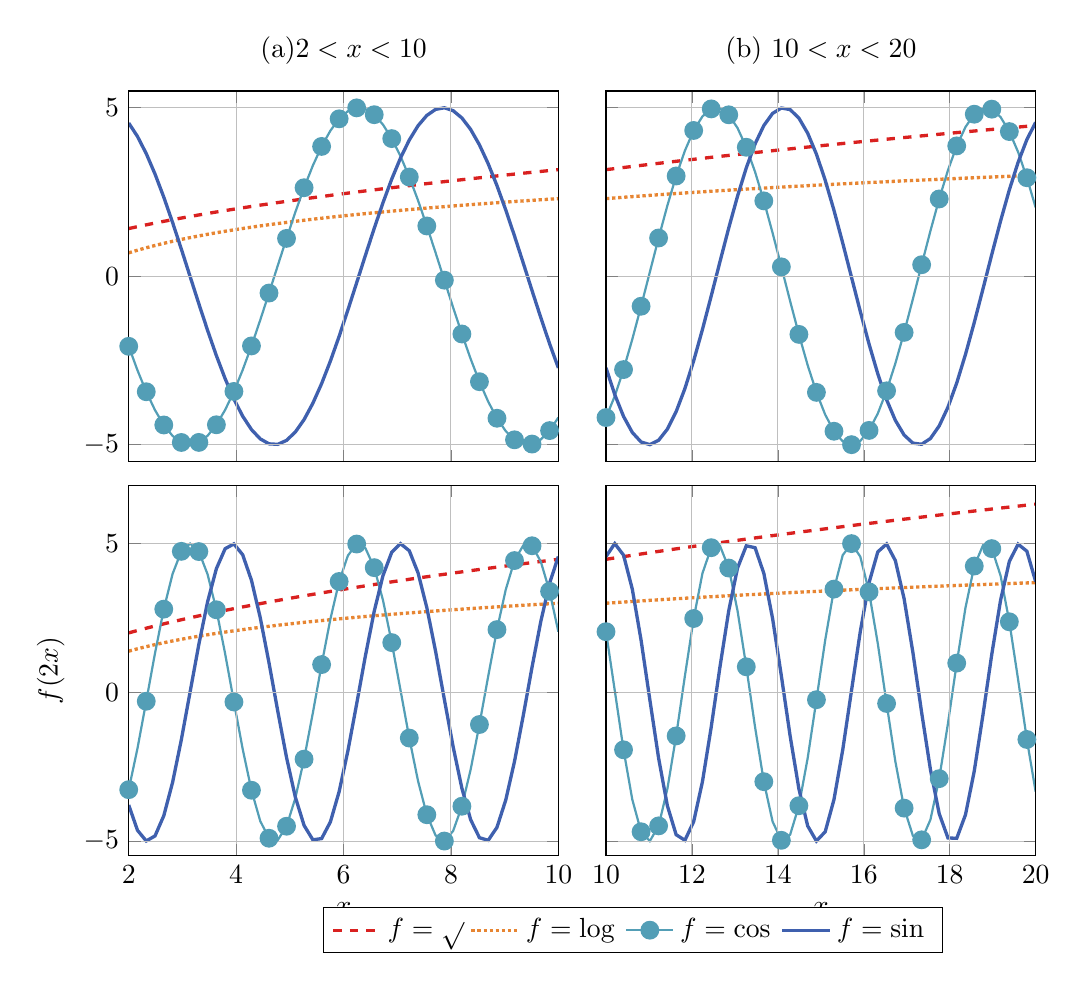
\begin{tikzpicture}[scale=1.]
\begin{groupplot}[group style={group size=2 by 2,
ylabels at=edge left, yticklabels at=edge left,horizontal sep=4.ex,
vertical sep=2ex,xticklabels at=edge bottom,xlabels at=edge bottom},
ymajorgrids=true,xmajorgrids=true,enlargelimits=0,xlabel=$x$,
axis on top,scale only axis,width=0.45\linewidth
]
\nextgroupplot[title={(a)$ 2<x<10$ },ymin=-5.499995602934542,ymax=5.498472401782701,]
\addplot[Red,dashed,mark=none,very thick,mark size=3pt,mark repeat=2] coordinates{(2.0,1.4142135623730951) (2.163265306122449,1.4708043058552858) (2.326530612244898,1.52529689314733) (2.489795918367347,1.5779087167410373) (2.6530612244897958,1.6288220358559113) (2.816326530612245,1.6781914463529615) (2.979591836734694,1.7261494247992246) (3.142857142857143,1.7728105208558367) (3.3061224489795915,1.8182745801939793) (3.4693877551020407,1.8626292586293283) (3.63265306122449,1.9059520091609048) (3.7959183673469385,1.9483116709979793) (3.9591836734693877,1.9897697538834456) (4.122448979591836,2.030381486221699) (4.285714285714286,2.0701966780270626) (4.448979591836734,2.1092604371762) (4.612244897959183,2.147613768338987) (4.775510204081632,2.1852940772540506) (4.938775510204081,2.2223355980148636) (5.1020408163265305,2.2587697572631282) (5.26530612244898,2.294625486315573) (5.428571428571429,2.32992949004287) (5.591836734693877,2.3647064796066926) (5.755102040816326,2.3989793748209522) (5.918367346938775,2.4327694808466287) (6.081632653061225,2.4660966430902955) (6.244897959183673,2.498979383505129) (6.408163265306122,2.531435020952764) (6.571428571428571,2.5634797778466227) (6.73469387755102,2.5951288749407073) (6.897959183673469,2.626396615835748) (7.061224489795918,2.657296462534039) (7.224489795918367,2.6878411031752543) (7.387755102040816,2.718042512920064) (7.551020408163265,2.747912008810192) (7.7142857142857135,2.7774602993176543) (7.877551020408163,2.806697529198357) (8.040816326530612,2.835633320182744) (8.204081632653061,2.864276807966203) (8.367346938775508,2.892636675902369) (8.53061224489796,2.920721185751553) (8.693877551020407,2.948538205792899) (8.857142857142858,2.9760952365713798) (9.020408163265305,3.0033994345183768) (9.183673469387754,3.0304576336566322) (9.346938775510203,3.0572763655760995) (9.510204081632653,3.083861877846129) (9.673469387755102,3.1102201510110343) (9.83673469387755,3.136356914300021) (10.0,3.1622776601683795) };
\addplot[Orange,densely dotted,mark=none,very thick,mark size=3pt,mark repeat=2] coordinates{(2.0,0.6931471805599453) (2.163265306122449,0.7716187960014406) (2.326530612244898,0.8443781502838689) (2.489795918367347,0.91220074662263) (2.6530612244897958,0.9757141523449557) (2.816326530612245,1.0354333870465782) (2.979591836734694,1.0917863235977099) (3.142857142857143,1.1451323043030026) (3.3061224489795915,1.1957760371217574) (3.4693877551020407,1.2439781389396352) (3.63265306122449,1.2899632521814586) (3.7959183673469385,1.3339263756025745) (3.9591836734693877,1.3760378609527015) (4.122448979591836,1.4164473992905782) (4.285714285714286,1.455287232606842) (4.448979591836734,1.4926747646784622) (4.612244897959183,1.528714701161659) (4.775510204081632,1.5635008172470748) (4.938775510204081,1.5971174280460598) (5.1020408163265305,1.6296406197516198) (5.26530612244898,1.6611392868109909) (5.428571428571429,1.6916760106710724) (5.591836734693877,1.7213078082774436) (5.755102040816326,1.750086772827487) (5.918367346938775,1.7780606248698931) (6.081632653061225,1.805273188394778) (6.244897959183673,1.831764803841754) (6.408163265306122,1.8575726877976266) (6.571428571428571,1.8827312474337816) (6.73469387755102,1.9072723563498992) (6.897959183673469,1.931225597372392) (7.061224489795918,1.9546184769470976) (7.224489795918367,1.9774766150231478) (7.387755102040816,1.9998239137151443) (7.551020408163265,2.0216827075276433) (7.7142857142857135,2.043073897508961) (7.877551020408163,2.064017071354204) (8.040816326530612,2.084530611187307) (8.204081632653061,2.104631790508394) (8.367346938775508,2.1243368615877265) (8.53061224489796,2.14366113441413) (8.693877551020407,2.1626190481587435) (8.857142857142858,2.181224235989778) (9.020408163265305,2.1994895839670714) (9.183673469387754,2.2174272846537386) (9.346938775510203,2.2350488860035584) (9.510204081632653,2.252365336015019) (9.673469387755102,2.26938702358445) (9.83673469387755,2.2861238159399737) (10.0,2.302585092994046) };
\addplot[Duck,solid,mark=*,thick,mark size=3pt,mark repeat=2] coordinates{(2.0,-2.080734182735712) (2.163265306122449,-2.792054502196311) (2.326530612244898,-3.429116215309583) (2.489795918367347,-3.9749757721069274) (2.6530612244897958,-4.41511527191081) (2.816326530612245,-4.737828587269876) (2.979591836734694,-4.934532704840567) (3.142857142857143,-4.999996002667765) (3.3061224489795915,-4.932477392509917) (3.4693877551020407,-4.733772626523322) (3.63265306122449,-4.409166536714354) (3.7959183673469385,-3.967292477418361) (3.9591836734693877,-3.4199027091297345) (4.122448979591836,-2.7815558306472927) (4.285714285714286,-2.0692295727155354) (4.448979591836734,-1.3018692514581365) (4.612244897959183,-0.49988389111798315) (4.775510204081632,0.3153965825735388) (4.938775510204081,1.1222886416942863) (5.1020408163265305,1.8993318599753968) (5.26530612244898,2.6258596829438803) (5.428571428571429,3.2825490839311118) (5.591836734693877,3.851934487074578) (5.755102040816326,4.318872288809712) (5.918367346938775,4.670943623251028) (6.081632653061225,4.898784659352287) (6.244897959183673,4.996335645129313) (6.408163265306122,4.961002075264998) (6.571428571428571,4.793723695617932) (6.73469387755102,4.498949509362966) (6.897959183673469,4.084519449510451) (7.061224489795918,3.5614558648894907) (7.224489795918367,2.943670365318029) (7.387755102040816,2.2475938228237) (7.551020408163265,1.4917393695520367) (7.7142857142857135,0.6962100150457378) (7.877551020408163,-0.11783602149584776) (8.040816326530612,-0.9287480437383169) (8.204081632653061,-1.7149587088541398) (8.367346938775508,-2.455557641261106) (8.53061224489796,-3.1308475733953007) (8.693877551020407,-3.7228682221743914) (8.857142857142858,-4.215873967922072) (9.020408163265305,-4.596752631212149) (9.183673469387754,-4.855374209675019) (9.346938775510203,-4.984860299621604) (9.510204081632653,-4.981767036838928) (9.673469387755102,-4.8461766909901085) (9.83673469387755,-4.581695477537261) (10.0,-4.195357645382262) };
\addplot[Blue,solid,mark=none,very thick,mark size=3pt,mark repeat=2] coordinates{(2.0,4.546487134128409) (2.163265306122449,4.147822519921183) (2.326530612244898,3.638840746982599) (2.489795918367347,3.0330788995940967) (2.6530612244897958,2.346648063886005) (2.816326530612245,1.5978048309002983) (2.979591836734694,0.8064657369404081) (3.142857142857143,-0.00632244465188645) (3.3061224489795915,-0.8189424719591597) (3.4693877551020407,-1.6097815753630935) (3.63265306122449,-2.35780627947216) (3.7959183673469385,-3.0431218179066843) (3.9591836734693877,-3.647501262520289) (4.122448979591836,-4.154870294123759) (4.285714285714286,-4.551734721553914) (4.448979591836734,-4.827539378618038) (4.612244897959183,-4.974948853546209) (4.775510204081632,-4.990042584557864) (4.938775510204081,-4.872419132702357) (5.1020408163265305,-4.625206858691015) (5.26530612244898,-4.254980719755363) (5.428571428571429,-3.771587399435816) (5.591836734693877,-3.1878834212194) (5.755102040816326,-2.5193932112617032) (5.918367346938775,-1.7838962044946904) (6.081632653061225,-1.0009539756126165) (6.244897959183673,-0.19138997155089457) (6.408163265306122,0.623264317297552) (6.571428571428571,1.421342017274927) (6.73469387755102,2.1816171323590967) (6.897959183673469,2.883869079304891) (7.061224489795918,3.5094204824221693) (7.224489795918367,4.041633924584019) (7.387755102040816,4.466354442675228) (7.551020408163265,4.772285998693759) (7.7142857142857135,4.951291913728175) (7.877551020408163,4.998611274347909) (8.040816326530612,4.912985555774844) (8.204081632653061,4.696692094115319) (8.367346938775508,4.355483517411608) (8.53061224489796,3.8984347464289764) (8.693877551020407,3.3377016344071393) (8.857142857142858,2.6881976650903128) (9.020408163265305,1.9671973077056064) (9.183673469387754,1.193876578220163) (9.346938775510203,0.3888030262953284) (9.510204081632653,-0.42661128755002103) (9.673469387755102,-1.230679275727092) (9.83673469387755,-2.002015622095545) (10.0,-2.7201055544468487) };
\nextgroupplot[title={(b) $10<x<20$},ymin=-5.499995602934542,ymax=5.498472401782701,]
\addplot[Red,dashed,mark=none,very thick,mark size=3pt,mark repeat=2] coordinates{(10.0,3.1622776601683795) (10.204081632653061,3.1943828249996997) (10.408163265306122,3.226168511610347) (10.612244897959183,3.2576440717118227) (10.816326530612244,3.2888184094918107) (11.020408163265307,3.319700011034929) (11.224489795918368,3.3502969713024497) (11.428571428571429,3.3806170189140663) (11.63265306122449,3.4106675389466634) (11.83673469387755,3.440455593940656) (12.040816326530612,3.469987943283177) (12.244897959183675,3.499271061118826) (12.448979591836736,3.52831115292242) (12.653061224489797,3.557114170853924) (12.857142857142858,3.585685828003181) (13.061224489795919,3.614031611621005) (13.26530612244898,3.6421567954234177) (13.46938775510204,3.67006645104718) (13.673469387755102,3.697765458727081) (13.877551020408163,3.7252585172586565) (14.081632653061224,3.7525501533039134) (14.285714285714285,3.779644730092272) (14.489795918367347,3.806546455564065) (14.693877551020408,3.8332593899996397) (14.89795918367347,3.8597874531732272) (15.10204081632653,3.8861344310672696) (15.306122448979592,3.912303982179758) (15.510204081632654,3.938299643454349) (15.714285714285715,3.9641248358604595) (15.918367346938776,3.989782869648269) (16.122448979591837,4.015276949301485) (16.3265306122449,4.040610178208843) (16.53061224489796,4.06578556307363) (16.73469387755102,4.090806018078958) (16.93877551020408,4.115674368825124) (17.142857142857142,4.140393356054125) (17.346938775510203,4.164965639175215) (17.551020408163264,4.189393799604337) (17.755102040816325,4.213680343929322) (17.95918367346939,4.2378277069118075) (18.163265306122447,4.261838254336085) (18.367346938775512,4.285714285714286) (18.57142857142857,4.309458036856673) (18.775510204081634,4.333071682315172) (18.979591836734695,4.356557337707688) (19.183673469387756,4.3799170619302545) (19.387755102040817,4.403152859263555) (19.591836734693878,4.426266681379905) (19.79591836734694,4.449260429256411) (20.0,4.47213595499958) };
\addplot[Orange,densely dotted,mark=none,very thick,mark size=3pt,mark repeat=2] coordinates{(10.0,2.302585092994046) (10.204081632653061,2.322787800311565) (10.408163265306122,2.3425904276077447) (10.612244897959183,2.3620085134648465) (10.816326530612244,2.381056708435541) (11.020408163265307,2.3997488414476935) (11.224489795918368,2.41809798011589) (11.428571428571429,2.436116485618568) (11.63265306122449,2.4538160627179693) (11.83673469387755,2.4712078054298385) (12.040816326530612,2.4883022387891387) (12.244897959183675,2.50510935710552) (12.448979591836736,2.5216386590567303) (12.653061224489797,2.5378991799285107) (12.857142857142858,2.553899521274952) (13.061224489795919,2.569647878243091) (13.26530612244898,2.5851520647790562) (13.46938775510204,2.6004195369098446) (13.673469387755102,2.615457414274385) (13.877551020408163,2.630272500059526) (14.081632653061224,2.6448712994806782) (14.285714285714285,2.659260036932778) (14.489795918367347,2.6734446719247345) (14.693877551020408,2.6874309138994743) (14.89795918367347,2.7012242360318104) (15.10204081632653,2.7148298880875887) (15.306122448979592,2.7282529084197296) (15.510204081632654,2.74149813516975) (15.714285714285715,2.754570216737103) (15.918367346938776,2.7674736215730107) (16.122448979591837,2.7802126473504405) (16.3265306122449,2.7927914295573006) (16.53061224489796,2.8052139495558577) (16.73469387755102,2.8174840421476723) (16.93877551020408,2.829605402680017) (17.142857142857142,2.841581593726733) (17.346938775510203,2.8534160513737357) (17.551020408163264,2.8651120911369268) (17.755102040816325,2.8766729135380027) (17.95918367346939,2.888101609361626) (18.163265306122447,2.8994011646155586) (18.367346938775512,2.910574465213684) (18.57142857142857,2.921624301400269) (18.775510204081634,2.9325533719324595) (18.979591836734695,2.9433642880366753) (19.183673469387756,2.954059577153423) (19.387755102040817,2.9646416864839598) (19.591836734693878,2.9751129863512555) (19.79591836734694,2.985475773386802) (20.0,2.995732273553991) };
\addplot[Duck,solid,mark=*,thick,mark size=3pt,mark repeat=2] coordinates{(10.0,-4.195357645382262) (10.204081632653061,-3.55701539427296) (10.408163265306122,-2.7710393690209267) (10.612244897959183,-1.8700514714544436) (10.816326530612244,-0.8914471663187101) (11.020408163265307,0.12415661591358101) (11.224489795918368,1.134607283030977) (11.428571428571429,2.097966122647882) (11.63265306122449,2.9742489666959218) (11.83673469387755,3.7270857326357754) (12.040816326530612,4.32522996220132) (12.244897959183675,4.743855704334085) (12.448979591836736,4.965587915236426) (12.653061224489797,4.981223608832654) (12.857142857142858,4.790113826318521) (13.061224489795919,4.400190571169072) (13.26530612244898,3.827637591668451) (13.46938775510204,3.096218675118909) (13.673469387755102,2.236291332849595) (13.877551020408163,1.283546812987282) (14.081632653061224,0.27752873670593103) (14.285714285714285,-0.7400081581048336) (14.489795918367347,-1.7268310454774243) (14.693877551020408,-2.6419818830294917) (14.89795918367347,-3.4474773737881863) (15.10204081632653,-4.109885461331396) (15.306122448979592,-4.601712925881628) (15.510204081632654,-4.902546489235054) (15.714285714285715,-4.9999000670136855) (15.918367346938776,-4.889733003071676) (16.122448979591837,-4.576617776758472) (16.3265306122449,-4.073550222355985) (16.53061224489796,-3.4014101375240084) (16.73469387755102,-2.5880946681776624) (16.93877551020408,-1.6673604386210175) (17.142857142857142,-0.6774224842769476) (17.346938775510203,0.3406318617487481) (17.551020408163264,1.3445482966975897) (17.755102040816325,2.292659311214952) (17.95918367346939,3.1456135975710993) (18.163265306122447,3.868009324031237) (18.367346938775512,4.429863486390934) (18.57142857142857,4.807856351302774) (18.775510204081634,4.986299340827026) (18.979591836734695,4.957786186198242) (19.183673469387756,4.72350032469852) (19.387755102040817,4.293165781142926) (19.591836734693878,3.6846435726390596) (19.79591836734694,2.9231903878241816) (20.0,2.0404103090669596) };
\addplot[Blue,solid,mark=none,very thick,mark size=3pt,mark repeat=2] coordinates{(10.0,-2.7201055544468487) (10.204081632653061,-3.5139210982754268) (10.408163265306122,-4.16189149490182) (10.612244897959183,-4.637122760302025) (10.816326530612244,-4.919890440819017) (11.020408163265307,-4.9984582757811316) (11.224489795918368,-4.869565310506992) (11.428571428571429,-4.538561242092235) (11.63265306122449,-4.019184380456841) (11.83673469387755,-3.332991440370474) (12.040816326530612,-2.5084628309137784) (12.244897959183675,-1.579820577298878) (12.448979591836736,-0.5856079371541699) (12.653061224489797,0.4329103357604186) (12.857142857142858,1.4334606834204213) (13.061224489795919,2.3745153057823805) (13.26530612244898,3.2170157703757907) (13.46938775510204,3.925994130897919) (13.673469387755102,4.472024270352497) (13.877551020408163,4.832443230796425) (14.081632653061224,4.9922918384548005) (14.285714285714285,4.944935583598465) (14.489795918367347,4.692339985590915) (14.693877551020408,4.2449890140899) (14.89795918367347,3.6214499523282813) (15.10204081632653,2.8476027628053764) (15.306122448979592,1.9555659405333126) (15.510204081632654,0.9823634362541417) (15.714285714285715,-0.03161202107648384) (15.918367346938776,-1.0442754228036069) (16.122448979591837,-2.0135962170848303) (16.3265306122449,-2.8993427851745137) (16.53061224489796,-3.664752253065534) (16.73469387755102,-4.2780563330267585) (16.93877551020408,-4.713799865047468) (17.142857142857142,-4.953897332181608) (17.346938775510203,-4.988383499166998) (17.551020408163264,-4.815827019095226) (17.755102040816325,-4.443389841404802) (17.95918367346939,-3.8865299554713078) (18.163265306122447,-3.168359807409413) (18.367346938775512,-2.3186870189700803) (18.57142857142857,-1.372777223455278) (18.775510204081634,-0.36989036709268963) (18.979591836734695,0.6483487733788728) (19.183673469387756,1.639678225315253) (19.387755102040817,2.562952901561683) (19.591836734693878,3.3798523255624153) (19.79591836734694,4.05647112112638) (20.0,4.564726253638138) };
\nextgroupplot[ylabel=$f(2x)$,ymin=-5.493890455696734,ymax=6.957010852370436,]
\addplot[Red,dashed,mark=none,very thick,mark size=3pt,mark repeat=2] coordinates{(2.0,2.0) (2.163265306122449,2.080031396937291) (2.326530612244898,2.1570955529345) (2.489795918367347,2.2314999074019015) (2.6530612244897958,2.3035022137995855) (2.816326530612245,2.3733211036908783) (2.979591836734694,2.4411439272335804) (3.142857142857143,2.5071326821120348) (3.3061224489795915,2.571428571428571) (3.4693877551020407,2.634155559226539) (3.63265306122449,2.695423180587601) (3.7959183673469385,2.75532878885513) (3.9591836734693877,2.813959371941744) (4.122448979591836,2.8713930346059686) (4.285714285714286,2.9277002188455996) (4.448979591836734,2.9829447168315855) (4.612244897959183,3.037184517924185) (4.775510204081632,3.0904725218262765) (4.938775510204081,3.142857142857143) (5.1020408163265305,3.1943828249996997) (5.26530612244898,3.245090483314442) (5.428571428571429,3.295017884191656) (5.591836734693877,3.344199974491321) (5.755102040816326,3.3926691677251193) (5.918367346938775,3.440455593940656) (6.081632653061225,3.487587318781058) (6.244897959183673,3.534090536243709) (6.408163265306122,3.5799897388976194) (6.571428571428571,3.625307868699863) (6.73469387755102,3.67006645104718) (6.897959183673469,3.714285714285714) (7.061224489795918,3.757984696561687) (7.224489795918367,3.801181341614306) (7.387755102040816,3.843892584878203) (7.551020408163265,3.8861344310672696) (7.7142857142857135,3.9279220242478625) (7.877551020408163,3.9692697112713726) (8.040816326530612,4.010191099319486) (8.204081632653061,4.050699108216522) (8.367346938775508,4.090806018078958) (8.53061224489796,4.130523512800274) (8.693877551020407,4.16986271980755) (8.857142857142858,4.20883424647321) (9.020408163265305,4.247448213519573) (9.183673469387754,4.285714285714286) (9.346938775510203,4.323641700120445) (9.510204081632653,4.361239292135356) (9.673469387755102,4.3985155195259) (9.83673469387755,4.435478484645721) (10.0,4.47213595499958) };
\addplot[Orange,densely dotted,mark=none,very thick,mark size=3pt,mark repeat=2] coordinates{(2.0,1.3862943611198906) (2.163265306122449,1.4647659765613859) (2.326530612244898,1.5375253308438142) (2.489795918367347,1.6053479271825752) (2.6530612244897958,1.6688613329049011) (2.816326530612245,1.7285805676065233) (2.979591836734694,1.7849335041576553) (3.142857142857143,1.8382794848629478) (3.3061224489795915,1.8889232176817026) (3.4693877551020407,1.9371253194995803) (3.63265306122449,1.9831104327414038) (3.7959183673469385,2.0270735561625197) (3.9591836734693877,2.0691850415126467) (4.122448979591836,2.1095945798505236) (4.285714285714286,2.1484344131667874) (4.448979591836734,2.1858219452384073) (4.612244897959183,2.2218618817216043) (4.775510204081632,2.25664799780702) (4.938775510204081,2.2902646086060052) (5.1020408163265305,2.322787800311565) (5.26530612244898,2.3542864673709363) (5.428571428571429,2.3848231912310176) (5.591836734693877,2.414454988837389) (5.755102040816326,2.4432339533874323) (5.918367346938775,2.4712078054298385) (6.081632653061225,2.498420368954723) (6.244897959183673,2.524911984401699) (6.408163265306122,2.550719868357572) (6.571428571428571,2.575878427993727) (6.73469387755102,2.6004195369098446) (6.897959183673469,2.6243727779323374) (7.061224489795918,2.6477656575070427) (7.224489795918367,2.670623795583093) (7.387755102040816,2.6929710942750895) (7.551020408163265,2.7148298880875887) (7.7142857142857135,2.7362210780689065) (7.877551020408163,2.7571642519141495) (8.040816326530612,2.7776777917472524) (8.204081632653061,2.7977789710683396) (8.367346938775508,2.817484042147672) (8.53061224489796,2.836808314974075) (8.693877551020407,2.855766228718689) (8.857142857142858,2.8743714165497236) (9.020408163265305,2.892636764527017) (9.183673469387754,2.910574465213684) (9.346938775510203,2.9281960665635034) (9.510204081632653,2.9455125165749645) (9.673469387755102,2.962534204144395) (9.83673469387755,2.979270996499919) (10.0,2.995732273553991) };
\addplot[Duck,solid,mark=*,thick,mark size=3pt,mark repeat=2] coordinates{(2.0,-3.2682181043180596) (2.163265306122449,-1.8817726627061244) (2.326530612244898,-0.2964647927603521) (2.489795918367347,1.3201729555348258) (2.6530612244897958,2.797297145704026) (2.816326530612245,3.9788078889406675) (2.979591836734694,4.739845206056465) (3.142857142857143,4.99998401067745) (3.3061224489795915,4.7317332910485685) (3.4693877551020407,3.963441311848607) (3.63265306122449,2.7762998193926602) (3.7959183673469385,1.2957638405521263) (3.9591836734693877,-0.3217061840348404) (4.122448979591836,-1.9051788643968206) (4.285714285714286,-3.2873155901597935) (4.448979591836734,-4.322054580843132) (4.612244897959183,-4.900046438160298) (4.775510204081632,-4.960209998280373) (4.938775510204081,-4.496187281889598) (5.1020408163265305,-3.55701539427296) (5.26530612244898,-2.2419443701959456) (5.428571428571429,-0.6899486046332081) (5.591836734693877,0.9349597170857968) (5.755102040816326,2.461063138819376) (5.918367346938775,3.7270857326357754) (6.081632653061225,4.599236455482119) (6.244897959183673,4.9853479515159) (6.408163265306122,4.844616636313447) (6.571428571428571,4.191914747971537) (6.73469387755102,3.096218675118909) (6.897959183673469,1.6733196533716646) (7.061224489795918,0.07358715102229982) (7.224489795918367,-1.533921912139368) (7.387755102040816,-2.9793288030418985) (7.551020408163265,-4.109885461331396) (7.7142857142857135,-4.806116645980005) (7.877551020408163,-4.9944458688152125) (8.040816326530612,-4.6549708285008995) (8.204081632653061,-3.8235666507701365) (8.367346938775508,-2.5880946681776775) (8.53061224489796,-1.0791173888659034) (8.693877551020407,0.5438991198703653) (8.857142857142858,2.1094373253611964) (9.020408163265305,3.4520539010223255) (9.183673469387754,4.429863486390926) (9.346938775510203,4.939532882697438) (9.510204081632653,4.9272011237339655) (9.673469387755102,4.3941714081183365) (9.83673469387755,3.3967733795541557) (10.0,2.0404103090669596) };
\addplot[Blue,solid,mark=none,very thick,mark size=3pt,mark repeat=2] coordinates{(2.0,-3.7840124765396412) (2.163265306122449,-4.632378616422875) (2.326530612244898,-4.991203124162907) (2.489795918367347,-4.82256605631011) (2.6530612244897958,-4.144288681865214) (2.816326530612245,-3.0280501618869375) (2.979591836734694,-1.591812621706317) (3.142857142857143,0.012644879194608175) (3.3061224489795915,1.6157660914818965) (3.4693877551020407,3.0481359824541614) (3.63265306122449,4.158384219001448) (3.7959183673469385,4.829181718419551) (3.9591836734693877,4.989639779698906) (4.122448979591836,4.6228014768812695) (4.285714285714286,3.767433637198188) (4.448979591836734,2.5139300308904566) (4.612244897959183,0.9947587164094516) (4.775510204081632,-0.6295369512263917) (4.938775510204081,-2.1873042600823127) (5.1020408163265305,-3.5139210982754268) (5.26530612244898,-4.469192929483656) (5.428571428571429,-4.9521683051936645) (5.591836734693877,-4.911807236387321) (5.755102040816326,-4.352375009893394) (5.918367346938775,-3.332991440370474) (6.081632653061225,-1.9613831921795075) (6.244897959183673,-0.3824994147920079) (6.408163265306122,1.236806228620711) (6.571428571428571,2.7254083631152834) (6.73469387755102,3.925994130897919) (6.897959183673469,4.7116877377050495) (7.061224489795918,4.999458463794296) (7.224489795918367,4.758895204504792) (7.387755102040816,4.015420262359212) (7.551020408163265,2.8476027628053764) (7.7142857142857135,1.3788556071010127) (7.877551020408163,-0.23560658622937886) (8.040816326530612,-1.8251702895361976) (8.204081632653061,-3.2218532038437813) (8.367346938775508,-4.27805633302675) (8.53061224489796,-4.882161986358834) (8.693877551020407,-4.970329339933547) (8.857142857142858,-4.533241022753257) (9.020408163265305,-3.6170877601236806) (9.183673469387754,-2.3186870189700963) (9.346938775510203,-0.7752515080609269) (9.510204081632653,0.8501112199440432) (9.673469387755102,2.385635688045289) (9.83673469387755,3.6690503686856415) (10.0,4.564726253638138) };
\nextgroupplot[legend style={at={($(0.62,-0.35)+(0.9cm,1cm)$)},legend columns=4},ymin=-5.493890455696734,ymax=6.957010852370436]
\addplot[Red,dashed,mark=none,very thick,mark size=3pt,mark repeat=2] coordinates{(10.0,4.47213595499958) (10.204081632653061,4.5175395145262565) (10.408163265306122,4.562491263620375) (10.612244897959183,4.607004427599171) (10.816326530612244,4.65109159888563) (11.020408163265307,4.69476477861571) (11.224489795918368,4.738035414793428) (11.428571428571429,4.780914437337574) (11.63265306122449,4.823412290324038) (11.83673469387755,4.865538961693257) (12.040816326530612,4.907304010662191) (12.244897959183675,4.948716593053935) (12.448979591836736,4.989785484735138) (12.653061224489797,5.030519103331145) (12.857142857142858,5.0709255283711) (13.061224489795919,5.1110125199995196) (13.26530612244898,5.150787536377128) (13.46938775510204,5.190257749881415) (13.673469387755102,5.229430062206608) (13.877551020408163,5.268311118453078) (14.081632653061224,5.306907320287631) (14.285714285714285,5.3452248382484875) (14.489795918367347,5.383269623261935) (14.693877551020408,5.421047417431508) (14.89795918367347,5.458563764155086) (15.10204081632653,5.495824017620384) (15.306122448979592,5.532833351724881) (15.510204081632654,5.569596768462265) (15.714285714285715,5.606119105813881) (15.918367346938776,5.642405045180428) (16.122448979591837,5.678459118386226) (16.3265306122449,5.714285714285714) (16.53061224489796,5.7498890849994595) (16.73469387755102,5.785273351804739) (16.93877551020408,5.820442510703818) (17.142857142857142,5.855400437691199) (17.346938775510203,5.890150893739515) (17.551020408163264,5.924697529522206) (17.755102040816325,5.959043889889774) (17.95918367346939,5.993193418115152) (18.163265306122447,6.027149459922567) (18.367346938775512,6.0609152673132645) (18.57142857142857,6.09449400220044) (18.775510204081634,6.127888739864919) (18.979591836734695,6.161102472242236) (19.183673469387756,6.194138111051085) (19.387755102040817,6.226998490772391) (19.591836734693878,6.2596863714876125) (19.79591836734694,6.292204441584355) (20.0,6.324555320336759) };
\addplot[Orange,densely dotted,mark=none,very thick,mark size=3pt,mark repeat=2] coordinates{(10.0,2.995732273553991) (10.204081632653061,3.0159349808715104) (10.408163265306122,3.03573760816769) (10.612244897959183,3.0551556940247915) (10.816326530612244,3.0742038889954864) (11.020408163265307,3.092896022007639) (11.224489795918368,3.1112451606758356) (11.428571428571429,3.1292636661785136) (11.63265306122449,3.1469632432779147) (11.83673469387755,3.1643549859897835) (12.040816326530612,3.1814494193490837) (12.244897959183675,3.1982565376654652) (12.448979591836736,3.2147858396166757) (12.653061224489797,3.231046360488456) (12.857142857142858,3.247046701834897) (13.061224489795919,3.2627950588030363) (13.26530612244898,3.2782992453390016) (13.46938775510204,3.29356671746979) (13.673469387755102,3.3086045948343306) (13.877551020408163,3.323419680619471) (14.081632653061224,3.3380184800406236) (14.285714285714285,3.3524072174927233) (14.489795918367347,3.36659185248468) (14.693877551020408,3.3805780944594197) (14.89795918367347,3.3943714165917553) (15.10204081632653,3.407977068647534) (15.306122448979592,3.421400088979675) (15.510204081632654,3.4346453157296954) (15.714285714285715,3.4477173972970485) (15.918367346938776,3.460620802132956) (16.122448979591837,3.473359827910386) (16.3265306122449,3.485938610117246) (16.53061224489796,3.498361130115803) (16.73469387755102,3.5106312227076173) (16.93877551020408,3.522752583239962) (17.142857142857142,3.5347287742866778) (17.346938775510203,3.5465632319336806) (17.551020408163264,3.558259271696872) (17.755102040816325,3.569820094097948) (17.95918367346939,3.581248789921571) (18.163265306122447,3.592548345175504) (18.367346938775512,3.6037216457736294) (18.57142857142857,3.614771481960214) (18.775510204081634,3.625700552492405) (18.979591836734695,3.6365114685966202) (19.183673469387756,3.647206757713368) (19.387755102040817,3.657788867043905) (19.591836734693878,3.6682601669112005) (19.79591836734694,3.678622953946747) (20.0,3.6888794541139363) };
\addplot[Duck,solid,mark=*,thick,mark size=3pt,mark repeat=2] coordinates{(10.0,2.0404103090669596) (10.204081632653061,0.06094340603792867) (10.408163265306122,-1.9285363261344424) (10.612244897959183,-3.601162997644428) (10.816326530612244,-4.682128779864937) (11.020408163265307,-4.993834053889955) (11.224489795918368,-4.485066525317226) (11.428571428571429,-3.239415259288725) (11.63265306122449,-1.4615372336432975) (11.83673469387755,0.5564672233668613) (12.040816326530612,2.4830456903696128) (12.244897959183675,4.001666777417216) (12.448979591836736,4.862825337576815) (12.653061224489797,4.925035456476721) (12.857142857142858,4.178076187635144) (13.061224489795919,2.7446708250420833) (13.26530612244898,0.8603238132613834) (13.46938775510204,-1.1653719663379634) (13.673469387755102,-2.9996004298487127) (13.877551020408163,-4.341003031548077) (14.081632653061224,-4.969191120120964) (14.285714285714285,-4.780955170375317) (14.489795918367347,-3.807221816150138) (14.693877551020408,-2.207972691897577) (14.89795918367347,-0.24595990288740335) (15.10204081632653,1.756463402105275) (15.306122448979592,3.470304740890424) (15.510204081632654,4.613984831644382) (15.714285714285715,4.999600272049384) (15.918367346938776,4.563795536531339) (16.122448979591837,3.378172109816664) (16.3265306122449,1.6375245656225976) (16.53061224489796,-0.3721636305395627) (16.73469387755102,-2.3207063954201423) (16.93877551020408,-3.887963667088611) (17.142857142857142,-4.8164395111184195) (17.346938775510203,-4.953587973904633) (17.551020408163264,-4.276875951139044) (17.755102040816325,-2.897485313079753) (17.95918367346939,-1.042046037910323) (18.163265306122447,0.9845984523170357) (18.367346938775512,2.849476203223857) (18.57142857142857,4.246193077904968) (18.775510204081634,4.945272446532814) (18.979591836734695,4.831857547223245) (19.183673469387756,3.9245821269708085) (19.387755102040817,2.37250896975062) (19.591836734693878,0.4306393029561332) (19.79591836734694,-1.5819831826129245) (20.0,-3.3346903082613095) };
\addplot[Blue,solid,mark=none,very thick,mark size=3pt,mark repeat=2] coordinates{(10.0,4.564726253638138) (10.204081632653061,4.999628576330496) (10.408163265306122,4.61310607278652) (10.612244897959183,3.468663296487077) (10.816326530612244,1.7543289568266491) (11.020408163265307,-0.24823666572248737) (11.224489795918368,-2.210017706598494) (11.428571428571429,-3.808699092588881) (11.63265306122449,-4.7816219962136595) (11.83673469387755,-4.968937937760782) (12.040816326530612,-4.339871438134647) (12.244897959183675,-2.99777634297746) (12.448979591836736,-1.1631550783197113) (12.653061224489797,0.8625692739989872) (12.857142857142858,2.7465759356544623) (13.061224489795919,4.179327943840111) (13.26530612244898,4.925428198272247) (13.46938775510204,4.862294538597347) (13.673469387755102,4.0002996464329295) (13.877551020408163,2.4810668431322864) (14.081632653061224,0.5542017788774762) (14.285714285714285,-1.4637170692663002) (14.489795918367347,-3.241151345221393) (14.693877551020408,-4.486073627553895) (14.89795918367347,-4.9939467083832225) (15.10204081632653,-4.681328477800374) (15.306122448979592,-3.5995812263864035) (15.510204081632654,-1.9264329662242505) (15.714285714285715,0.06322277851949984) (15.918367346938776,2.0424911996717694) (16.122448979591837,3.686184096929619) (16.3265306122449,4.724247378893544) (16.53061224489796,4.986130186036423) (16.73469387755102,4.428805914268094) (16.93877551020408,3.1438413642228955) (17.142857142857142,1.342352575047763) (17.346938775510203,-0.6796809433751956) (17.551020408163264,-2.5900448062858867) (17.755102040816325,-4.074871637301857) (17.95918367346939,-4.890208590119178) (18.163265306122447,-4.902098110778169) (18.367346938775512,-4.108586784681681) (18.57142857142857,-2.6400462770852977) (18.775510204081634,-0.7377536374450182) (18.979591836734695,1.28574983699854) (19.183673469387756,3.098008251871076) (19.387755102040817,4.401272678266237) (19.591836734693878,4.981420459141093) (19.79591836734694,4.743134955905206) (20.0,3.725565802396744) };
\addlegendentry{$f=\sqrt{}$}
\addlegendentry{$f=\log{}$}
\addlegendentry{$f=\cos{}$}
\addlegendentry{$f=\sin{}$}

\end{groupplot}
\end{tikzpicture}
\end{document}




%%% Local Variables:
%%% mode: latex
%%% TeX-master: "../mainManuscript"
%%% End:


%% Chapter 3: Extension of the Material Point Method

\section*{Introduction}
It has been highlighted in the previous chapter that even though exact solutions of hyperbolic systems have been derived, it is not possible in general. It is indeed well known that in addition to the mathematical complexity of PDEs, physics often involves multidimensional problems in domains with complex geometries that cannot be solved analytically. Numerical strategies may then be employed in order to compute an approximate solution to such problems.

Since the early 50's, plenty of numerical methods consisting mainly in mesh-based schemes, that is methods subdividing a complex domain into elements of simple shapes in which an approximate solution is sought, have been developed (\textit{finite element \cite{Belytschko}, finite volume \cite{Leveque} etc.}). Problems involving very large deformations may lead, however, to numerical difficulties when this kind of approach is used with a material description (Lagrangian formulation) due to severe mesh distortions. Alternatively, Eulerian methods avoid mesh entanglement by building an approximate solution of a PDEs system on a fixed mesh that corresponds to a discretized volume of control. Nevertheless, interface tracking techniques and convection steps are required in Eulerian approaches in order to follow the boundaries and transport internal variables, which is less convenient for solid than for fluid mechanics because of history dependent constitutive behaviours.

The \textbf{Material Point Method} (MPM) \cite{Sulsky94} mixes the advantages of both Lagrangian and Eulerian methods in order to circumvent mesh entanglement. However, the MPM suffers from numerical diffusion and oscillations that make it unable to accurately capture discontinuous waves traveling in solids. These limitations have been the object of researches that yield significant improvements without allowing to capture discontinuities. This is the purpose of this chapter.

In what follows, a brief historical review of developments that led to the MPM formulation is made and the original formulation is recalled in section \ref{sec:MPM}. Next, after emphasizing some shortcomings of the method, an extension of the MPM to the Discontinuous Galerkin (DG) approximation is proposed in section \ref{sec:DGMPM}. At last, the numerical analysis of the \textbf{Discontinuous Galerkin Material Point Method} (DGMPM) is performed in section \ref{sec:DGMPM_analysis} in terms of convergence and stability. Those studies of the numerical scheme show that the optimal Courant number may be reached in specific cases at the cost of first-order accuracy in velocity.



\section{The material point method}
\label{sec:MPM}
% \subsection{Historical review}

The early developments that led to the original MPM started with the \textbf{Particle-In-Cell} method (PIC) formulated for fluid dynamics problems \cite{PIC}. The novelty brought by PIC was the representation of a fluid by a collection of moving particles inside a background control volume subdivided into cells. Every single particle is given a constant mass and a position which is updated based on the velocity field resulting from the solution of linear momentum balance equation on the fixed background mesh. On the other hand, velocity, energy and pressure are stored at cells during the whole computation ($C^0$ approximation). A \textit{convective phase}, which consists in a weighting procedure, must be followed when a particle leaves a cell and enters a new one \cite{PIC}. Thus, the PIC enables the merging of Lagrangian and Eulerian techniques since the moving particles with ascribed masses enables the simulation of problems involving several highly deformed fluids without mesh distortion.

In spite of the good results provided by the PIC, the numerical diffusion it suffers from has been addressed by two different ways. First the method has been extended to a \textit{fully Lagrangian} approach \cite{McCrory_FLIP} by storing not only mass and position but all the fields at particles. Next, a new projection procedure has been proposed between the grid and the particles in order to reach second-order accuracy in space of the convective phase \cite{PIC_Nishiguchi}. The merging of those two improvements yielded the so-called \textbf{FLuid Implicit Particle} method (FLIP) \cite{FLIP}. In this new PIC formulation, every quantities are stored at particles so that the grid is only used for solving balance equations and hence provides an adaptive feature to the numerical scheme. The projection of fields from Lagrangian particles to the Eulerian mesh is made as in PIC while the backward mapping models the \textit{collisional} behavior of the fluid and leads to a double definition of the velocity. Indeed, the linear momentum resulting from the solution of balance equations on the grid is used to update the position of particles, whereas the change of linear momentum is used to update their velocity \cite{Mass_Flip}. This procedure yields a time derivative of particles displacement that is different from their velocity which, although it introduces oscillations in the vicinity of discontinuities, provides better results in terms of numerical diffusion \cite{Mass_Flip}.

Even though particles carry the whole history of the problem, FLIP has been essentialy used until the 90's to model history-independent constitutive models wich were dealt with on the grid. The first application of the method to history-dependent materials was made in the context of solid mechanics and yields the \textbf{Material Point Method} (MPM) \cite{Sulsky94}. %Since this formulation was based on a weak formulation for which \textit{material points} plays the role of integration points, the MPM may be seen as an extension of the Finite Element Method with moving Gauss points. Indeed, each material point is ascribed a volume by means of a delta Dirac \textit{characteristic function} which allows to approximate the volume integrals of the weak form by discrete sums over the Lagrangian particles.

\subsection{Derivation of the MPM}
Consider a solid domain with volume $\Omega_t$ bounded by the surface $\partial \Omega_t$, subject to traction forces and prescribed velocity on its boundaries within the time interval $\tau$:
\begin{align}
  & \tens{\sigma}\cdot\vect{n}=\vect{T}^d \quad \text{on } \partial \Omega_t^\sigma\\
  & \vect{v} = \vect{v}^d \quad \text{on } \partial \Omega_t^v
\end{align}
where $\vect{n}$ is the outward normal vector to $\partial \Omega_t$ and the set of boundaries satisfies $\partial \Omega_t =\partial \Omega^\sigma_t \cap \partial \Omega^v_t$.
%We seek an approximate solution of the eulerian balance equation of linear momentum \eqref{eq:HPP_linear_momentum} in a finite-dimensional function space using Galerkin approach. 

\subsubsection*{Weak formulation of the continuum problem}
The weak form of the eulerian balance equation of linear momentum \eqref{eq:HPP_linear_momentum} is written based on the Galerkin approach and the following function spaces:
\begin{equation}
\Vscr^1 = \{ \vect{u} \in H^1(\Omega_t) \}  \quad ; \quad \Vscr^1_{h} = \{\vect{u} \in \Vscr^1 | \vect{u}=\vect{v}^d \text{ on } \partial \Omega_t^v \}  \quad ; \quad \Vscr^1_{h,0} = \{\vect{u} \in \Vscr_h^1 | \vect{u}=\vect{0} \text{ on } \partial \Omega_t^v \} 
\end{equation}
where $H^1(\Omega_t)$ denotes the \textit{Sobolev} space in $\Omega_t$ \cite{DiPietro}. Thus, multiplication of equation \eqref{eq:HPP_linear_momentum} by a test function $\vect{w} \in \Vscr^1_{h,0}$ and integration over $\Omega_t$ yields, after integration by parts, the following weak form:
\begin{equation}
  \label{eq:linear_momentum_weak_form}
  \begin{aligned}
    &\text{Find $\vect{v}\in \Vscr_h^1$ such that} \\
    &\int_{\Omega_t}  \rho  \vect{\dot{v}} \cdot \vect{w}\: dv + \int_{\Omega_t}\tens{\sigma}: 
    \nablat \vect{w} \:dv - \int_{\partial \Omega^\sigma_t} \vect{T}^d\cdot\vect{w}\: ds= \int_{\Omega_t} \rho \vect{b}\cdot \vect{w} \: dv  \qquad \forall \: \vect{w} \in \Vscr_{h,0}^1
  \end{aligned}
\end{equation}

\subsubsection{The MPM discretization}
The continuum body is discretized into a set of $N_p$ material points in an arbitrary Cartesian grid. The grid is here supposed to be made of $N_n$ nodes and $E$ non-overlapping cells or elements, which set of faces separating cells that contain particles and having empty neighboring elements defines the boundary of the mesh (see figure \ref{fig:domain} for a two-dimensional case).
\begin{figure}[h!]
  \centering
  {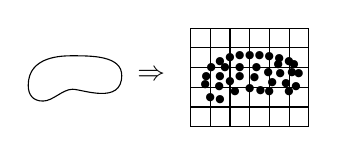
\begin{tikzpicture}[scale=0.25]
  % \draw[step=1.0,black,thin] (-3.,-1.) grid (3,4.);
  % \draw (-3,-1) -- (3,-1) -- (3,4) -- (-3,4) -- (-3,-1);
  \begin{scope}[scale=0.5]
    \draw (-3,0.6) .. controls +(1,0) and +(-1,0) .. (0,1.8)  
    .. controls +(1,0) and +(0,-3) .. (5,3.2) 
    .. controls +(0,2) and +(2,0)  .. (0,5.2) 
    .. controls +(-1,0) and +(0,3) .. (-4.5,2.2) 
    .. controls +(0,-1) and +(-1,0).. (-3,0.6) ;
    \begin{scope}  % pour limiter la portée du clip
      \clip (-3,0.6) .. controls +(1,0) and +(-1,0) .. (0,1.8) 
      .. controls +(1,0) and +(0,-3) .. (5,3.2)
      .. controls +(0,2) and +(2,0)  .. (0,5.2)
      .. controls +(-1,0) and +(0,3) .. (-4.5,2.2)
      .. controls +(0,-1) and +(-1,0).. (-3,0.6);
    \end{scope}
    %\node[below] at (0,1) {$\Omega$};
  \end{scope}
  \node at (4.,1.62) {$\Rightarrow$};
  \begin{scope}[shift={(9,0)}]
    \draw[step=1.0,black,thin] (-3.,-1.) grid (3,4.);
    % contour
    \node at (0,0.9) {\scriptsize$\bullet$}  ;
    \node at (2.5,1.65) {\scriptsize$\bullet$}  ; 
    \node at (0,2.6) {\scriptsize$\bullet$}  ;
    \node at (-2.25,1.1) {\scriptsize$\bullet$}  ; 
    \node at (-1.5,0.35) {\scriptsize$\bullet$}  ; 
    \node at (-2.,0.45) {\scriptsize$\bullet$} ;
    \node at (-2.2,1.5) {\scriptsize$\bullet$}  ; 
    \node at (-1.5,2.3) {\scriptsize$\bullet$} ; 
    \node at (2.35,1.) {\scriptsize$\bullet$}  ;
    \node at (2.25,2.15) {\scriptsize$\bullet$}  ;
    \node at (0.55,0.8) {\scriptsize$\bullet$}  ; 
    \node at (-0.5,2.6) {\scriptsize$\bullet$};
    \node at (0.5,2.59) {\scriptsize$\bullet$}  ;
    \node at (1.5,2.45) {\scriptsize$\bullet$}  ;
    \node at (1,0.75) {\scriptsize$\bullet$}; 
    \node at (2,0.75) {\scriptsize$\bullet$}  ;
    \node at (2,2.3) {\scriptsize$\bullet$}  ;
    \node at (1,2.55) {\scriptsize$\bullet$}  ;
    \node at (-1,2.5) {\scriptsize$\bullet$}  ; 
    \node at (-1.95,2.) {\scriptsize$\bullet$}  ;
    % interior
    \node at (-1.5,1.5) {\scriptsize$\bullet$}  ; 
    \node at (-1.25,2.) {\scriptsize$\bullet$}  ;
    \node at (-0.75,0.75) {\scriptsize$\bullet$}  ; 
    \node at (-1.55,1.){\scriptsize$\bullet$} ;
    \node at (-0.5,1.5) {\scriptsize$\bullet$}  ; 
    \node at (-0.5,2.) {\scriptsize$\bullet$}  ;
    \node at (0.25,1.45) {\scriptsize$\bullet$}  ;
    \node at (0.35,2.) {\scriptsize$\bullet$}  ;
    \node at (0.95,1.75) {\scriptsize$\bullet$}  ;
    \node at (1.15,1.2) {\scriptsize$\bullet$} ;
    \node at (1.45,2.15) {\scriptsize$\bullet$}  ; 
    \node at (1.55,1.65) {\scriptsize$\bullet$}  ;
    \node at (1.85,1.15) {\scriptsize$\bullet$}  ; 
    \node at (2.15,1.75) {\scriptsize$\bullet$}  ;
    \node at (-1.,1.25) {\scriptsize$\bullet$}  ;
    % \draw(3,0.5) -- (3.4,0.5) node [right]  {$\Omega_g$};
  \end{scope}
\end{tikzpicture}

%%% Local Variables:
%%% mode: latex
%%% TeX-master: "../presentation"
%%% End:
}
  {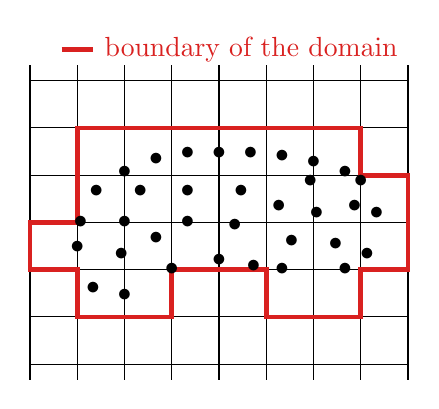
\begin{tikzpicture}[scale=0.8]
  \draw[step=.75,black,thin] (-3.,-1.) grid (3,4.);
  \draw[line width=0.6mm,Red] (-2.25,2.25) -- (-2.25,2.25)-- (-2.25,3)-- (2.25,3) --(2.25,2.25) -- (3.,2.25)-- (3.,0.75) --(2.25,0.75) --(2.25,0.) -- (0.75,0.) --(0.75,0.75) --(-0.75,0.75)-- (-0.75,0.)-- (-2.25,0.) -- (-2.25,0.75) --  (-3.,0.75)--(-3.,1.5) --(-2.25,1.5)--(-2.25,2.25);
  % contour
  \node at (0,0.9) {$\bullet$}  ; \node at (2.5,1.65) {$\bullet$}  ; 
  \node at (0,2.6) {$\bullet$}  ;\node at (-2.25,1.1) {$\bullet$}  ; 
  \node at (-1.5,0.35) {$\bullet$}  ; \node at (-2.,0.45) {$\bullet$}  ;
  \node at (-2.2,1.5) {$\bullet$}  ; \node at (-1.5,2.3) {$\bullet$}  ; 
  \node at (2.35,1.) {$\bullet$}  ; \node at (2.25,2.15) {$\bullet$}  ;
  \node at (0.55,0.8) {$\bullet$}  ; \node at (-0.5,2.6) {$\bullet$}  ; 
  \node at (0.5,2.59) {$\bullet$}  ; \node at (1.5,2.45) {$\bullet$}  ;
  \node at (1,0.75) {$\bullet$}; \node at (2,0.75) {$\bullet$}  ;
  \node at (2,2.3) {$\bullet$}  ; \node at (1,2.55) {$\bullet$}  ;
  \node at (-1,2.5) {$\bullet$}  ; \node at (-1.95,2.) {$\bullet$}  ;
  % interior
  \node at (-1.5,1.5) {$\bullet$}  ; \node at (-1.25,2.) {$\bullet$}  ;
  \node at (-0.75,0.75) {$\bullet$}  ; \node at (-1.55,1.) {$\bullet$}  ;
  \node at (-0.5,1.5) {$\bullet$}  ; \node at (-0.5,2.) {$\bullet$}  ;
  \node at (0.25,1.45) {$\bullet$}  ; \node at (0.35,2.) {$\bullet$}  ;
  \node at (0.95,1.75) {$\bullet$}  ; \node at (1.15,1.2) {$\bullet$}  ;
  \node at (1.45,2.15) {$\bullet$}  ; \node at (1.55,1.65) {$\bullet$}  ;
  \node at (1.85,1.15) {$\bullet$}  ; \node at (2.15,1.75) {$\bullet$}  ;
  \node at (-1.,1.25) {$\bullet$}  ;
  \draw[line width=0.6mm,Red] (-2.5,4.25) -- (-2.,4.25) node [right] {\text{boundary of the domain}};
\end{tikzpicture}}
  \caption{Representation of a continuum body by a set of material points in $\Rbb^2$.}
  \label{fig:domain}	
\end{figure}
Analogously to the Finite Element Method (FEM) \cite{Belytschko}, the velocity is approximated on the MPM background mesh by:
\begin{equation}
  \label{eq:approximation_basis}
  \vect{v}(\vect{x},t)=S_i(\vect{x})\vect{v}^{i}(t)
\end{equation}
where $\vect{v}^{i}$ is the velocity of the $i$th grid node, and $S_i(\vect{x})$ the (linear) shape function attached to it. One feature of the MPM is that the mass density is approximated on the grid based on the mass carried by each material point:
\begin{equation}
  \label{eq:density_approx}
  \rho\(\vect{x},t\)=\sum_{p=1}^{N_p} m_p \delta(\vect{x}_p-\vect{x})
\end{equation}
where the delta Dirac distribution $\delta$ is often referred to as the \textit{characteristic function} of material points, and $\vect{x}_p$ is the position of the $p$th particle. In what follows, the dependence on time will be omitted for simplicity and $p$ and $i$ or $j$ stand respectively for material points and nodes.

By introducing a specific Cauchy tensor $\rho \tens{\bar{\sigma}}=\tens{\sigma}$ and the approximation of mass density \eqref{eq:density_approx} in the weak form \eqref{eq:linear_momentum_weak_form}, the property of the delta Dirac distribution yields:
\begin{equation}
  \begin{aligned}
    &\text{Find $\vect{v}\in \Vscr_h^1$ such that} \\
    & \sum_{p=1}^{N_p} m_p  \[\vect{\dot{v}}(\vect{x}_p) \cdot \vect{w}(\vect{x}_p) + \tens{\bar{\sigma}}(\vect{x}_p):\nablat \vect{w}(\vect{x}_p) \]  = \sum_{p=1}^{N_p}m_p \vect{b}(\vect{x}_p)\cdot \vect{w}(\vect{x}_p) + \int_{\partial \Omega^\sigma_t} \vect{T}^d\cdot\vect{w}\: ds  \qquad \forall \: \vect{w} \in \Vscr_{h,0}^1
  \end{aligned}
\end{equation}
Then, with the approximation \eqref{eq:approximation_basis}, the weak form reads:
\begin{equation}
  \label{eq:mpm_discrete_weak}
    \begin{aligned}
      &\text{Find $\vect{v} \in \Vscr_h^1$ such that} \\
      & \vect{w}^j \sum_{p=1}^{N_p} m_p  \[ S_{jp} S_{ip} \vect{\dot{v}}^i + \nablav S_{jp} \cdot \tens{\bar{\sigma}}^p \]  =  \vect{w}^j\( \sum_{p=1}^{N_p}m_p S_{jp}\vect{b}^i  + \int_{\partial \Omega^\sigma_t} S_j(\vect{x})\vect{T}^d\: ds\)  \qquad \forall \: \vect{w} \in \Vscr_{h,0}^1
  \end{aligned}
\end{equation}
in which $S_{ip}=S_i(\vect{x}_p)$ and $\tens{\bar{\sigma}}^p=\tens{\bar{\sigma}}(\vect{x}_p)$. Next, the arbitrariness of the test function $\vect{w}$ yields the semi-discrete equation in matrix form:
\begin{equation}
  \label{eq:mpm_semi-discrete}
  m_{ji} \vect{\dot{v}}^i = \vect{f}_{int}^j + \vect{f}_{ext}^j 
\end{equation}
where the definition of the mass matrix $m_{ij}$ and the internal and external force vectors $\vect{f}_{int}^j $ and $\vect{f}_{ext}^j$ are:
\begin{subequations}
  \begin{alignat}{1}
    & m_{ij}= \sum_{p=1}^{N_p} m_p  S_{jp} S_{ip} \label{eq:mass_matrix}\\
    & \vect{f}_{int}^j = - \sum_{p=1}^{N_p} m_p \nablav S_{jp} \cdot \tens{\bar{\sigma}}^p \label{eq:int_forces}\\
    & \vect{f}_{ext}^j =\sum_{p=1}^{N_p}m_p S_{jp}\vect{b}^i  + \int_{\partial \Omega^\sigma_t} S_j(\vect{x})\vect{T}^d\: ds \label{eq:ext_forces}
  \end{alignat}
\end{subequations}
The system \eqref{eq:mpm_semi-discrete} can be solved for the nodal accelerations $\vect{\dot{v}}^i$, and advanced in time by using an explicit time discretization so that the nodal velocities can be updated. Hence, the time interval $\tau$ is discretized in $N_T$ sub-intervals of size $\Delta t^n$ such that $\sum_{n=1}^{N_T} \Delta t^n = T$ and time integration is performed with an explicit forward Euler algorithm leading to discrete equations:
\begin{equation}
  \label{eq:mpm_discrete}
  \frac{\vect{v}^{i,n+1}-\vect{v}^{i,n}}{\Delta t^n} = \vect{\dot{v}}^i
\end{equation}
where the superscripts $\bullet^{k,l}$ denote the time step $l$ at which the $k$th nodal field is evaluated. 

Note that in the weak form, the particles play the role of integration points so that the mass matrix depends on the positions of material points in the grid and must be computed at each time step. Hence, the MPM can be seen as an extension of the Finite Element Method with moving Gauss points. However, a consequence of this quadrature rule is that the consistent mass matrix $m_{ji}$ may be singular when only one material point lies in an element due to the reduced integration. The use of a linear combination of the diagonally lumped mass matrix $m^L_i=\sum_p S_{ip}m_p$ (positive-definite), and the constitent mass matrix (positive semi-definite) is then recommended \cite{Love}. Nevertheless, since no parameter value is prescribed for this combination, the lumped mass matrix is widely used in MPM simulations, though it introduces some dissipation of kinetic energy \cite{Mass_Flip}.  

Recall that the background grid inherited from FLIP is arbitrary and that the fields must be projected from particles to the nodes to solve the linear system \eqref{eq:mpm_discrete} and back so that the material points advect the solution. The first mapping step, required to build the discrete form,
aims at satify the conservation of linear momentum from particles to the grid:
\begin{equation}
  \label{eq:particles2nodes}
  m^{L,n}_i \vect{v}^{i,n} = \sum_{p=1}^{N_p} S_{ip}m_p \vect{v}^{p,n}
\end{equation}
to be solved for each $\vect{v}^i$. Once the nodal accelerations are calculeted for system \eqref{eq:mpm_semi-discrete}, the velocity of each material points is \textbf{updated} as:
\begin{equation}
  \label{eq:mp_velocity_update}
  \vect{v}^{p,n+1}= \vect{v}^{p,n}+ \Delta t\sum_{i=1}^{N_n} S_{ip}\vect{\dot{v}}^{i}
\end{equation}
while the updated nodal velocities resulting from the solution of \eqref{eq:mpm_discrete} are used to update the particles positions:
\begin{equation}
  \label{eq:position_update}
  \vect{x}^{p,n+1}=\vect{x}^{p,n} + \Delta t\sum_{i=1}^{N_n} S_{ip}\vect{v}^{i,n+1} 
\end{equation}

The integration of constitutive equations is performed at material points based on the nodal velocity field and the gradient of shape functions. Hence, one has some freedom in the way in which the stress is computed since it can be done right after either the resolution of \eqref{eq:mpm_discrete} or the projection \eqref{eq:particles2nodes}. The first option yields the \textit{Update Stress Last} (USL) algorithm while the second implementation is called \textit{Update Stress First} (USF) \cite{Bardenhagen_USF_USL}. 

The solution of discrete equations on the background grid requires the enforcement of boundary conditions at nodes. While Neumann boundary conditions are prescribed through the external force vector (equation \eqref{eq:ext_forces}), Dirichlet boundary conditions have to be imposed on both nodal acceleration and velocity in order to consistently update the kinematics and constitutive equations at material points. The enforcement of boundary condition is still a chalenging aspect of the material point method (as others mesh-free methods) for problems involving complex geometries, see for instance \cite{Bcs_MPM}. However, we consider here problems that do not require a particular treatment of boundary conditions.

\subsubsection{Solution scheme summary}
Let us assume that position and velocity vectors  $\vect{x}^n$ and $\vect{v}^n$ are known at every material points that discretize the continuum body in the grid at time $t^n$. Moreover, the USL implementation of the method also requires the knowledge of the specific stress tensor $\tens{\bar{\sigma}}^n$ at material points. The MPM solution scheme then consists of the following steps:
\begin{itemize}
\item[(a)] Computation of the consistent and lumped mass matrices and external forces (Neumann boundary conditions) from equations \eqref{eq:mass_matrix} and \eqref{eq:ext_forces}.
\item[(b)] Convective phase: projection of fields to the grid \eqref{eq:particles2nodes} and enforce Dirichlet boundary conditions on the nodal velocity. For USF formulation, the enforcement of Dirichlet boundary conditions on the mesh is required so that the integration of constitutive equations can be done.
\item[(c)] Evaluation of internal forces from equation \eqref{eq:int_forces}.
\item[(d)] Solution of the semi-discrete and discrete forms \eqref{eq:mpm_semi-discrete} and \eqref{eq:mpm_discrete} so that nodal accelerations $\vect{\dot{v}}^i$ and updated velocities $\vect{v}^{i,n+1}$ are determined. Enforcement of Dirichlet boundary conditions: set the velocity of boundary nodes to the prescribed values and their accelerations to zero.
\item[(e)] Update the material points velocities and positions with equations \eqref{eq:mp_velocity_update} and \eqref{eq:position_update} respectively. At this point the mesh has virtually moved, but since fields have been transferred back to particles, the underlying grid can be discarded and rebuilt for the next time step for computational convenience, thus involving the convective phase (b) at the next time step. 
\item[(f)] If the USL implementation is set, constitutive equations must be integrated.
\end{itemize}

Although the material point method has been successfully applied to a wide range of complex large strain engineering problems involving finite deformations \cite{Wieckowski}, this approach suffers from limitations which are discussed in the next section. 

\subsection{Shortcomings of the MPM}

%% Quick way
%The computation of internal forces within the MPM may lead to the well-known \textit{grid-crossing} instability due to the discontinuity of the gradient of shape functions when material points move from one cell to another \cite{Gimp}. The \textbf{Generalized Interpolation Material Point method} (GIMP) \cite{Gimp}, the \textbf{B-Spline Material Point Method} (BSMPM) \cite{Steffen_quadError} and the \textbf{Dual Domain Material Point Method} (DDMPM) \cite{DDMPM0} addressed this issue respectively by: (i) changing the particles characteristic function; (ii) enriching the approximation basis with quadratic or cubic B-Spline functions; (iii) introducing a modified gradient of shape functions. 

\subsubsection*{The grid-crossing instability}
The research on MPM mainly focused so far on the instability arising from the computation of internal forces when material points move from one cell to another due to the discontinuity of the gradient of shape functions across element interfaces, the so-called \textit{grid-crossing} error \cite{Gimp}. The \textbf{Generalized Interpolation Material Point Method} (GIMP) addressed this numerical issue by modifying the particles characteristic function, thus widening the domain of influence of material points \cite{Gimp}. By doing so, every particle are given a domain having either a constant shape (the uGIMP formulation) or not (the cpGIMP formulation), that must be tracked during the computation. In the cpGimp algorithm, only diagonal entries of the deformation gradient are used to update the "shapes" of particles. The \textbf{Convected Particle Domain Interpolation} (CPDI) \cite{CPDI} has then been developed to account for shear deformations an rotations of particles domains, thus providing an improvement of GIMP. However, those methods involve other difficulties related to the tracking of the deforming domains material points in the Eulerian grid which leads to mesh entanglement issues \cite{DDMPM0}. As a consequence, other ways consisting in the direct modification of the approximation basis have been followed to tackle the grid-crossing error. First, the \textbf{B-Spline Material Point Method} (BSMPM) \cite{Steffen_quadError} uses quadratic or cubic B-Spline functions with continuous gradients as nodal shape functions which allow to circumvent the instability \cite{MPM_BSpline1}. Second, the classical approximation basis is used and modified gradients with extended supports are introduced in the \textbf{Dual Domain Material Point Method} (DDMPM) \cite{DDMPM0}. These approaches both solve the grid-crossing error by widening the domain of influence of material points since B-Spline functions span more cells than Lagrange polynomials and the supports of the modified gradients of the DDMPM are larger than those of the shape functions.  

\subsubsection*{The back-mapping instability}
Numerical noise also appears in the MPM solution for problems that do not involve the grid-crossing instability. As an illustration of the previous remark, let us consider a one-dimensional elastic bar of length $L=6\:m$ with Young's modulus $E=200 \:GPa$ and mass density $\rho=7800 \:kg\cdot m^{-3}$ within the infinitesimal theory. The bar is initially in a free stress state and Riemann-type initial velocities are prescribed along the bar, that is: $v=v_0>0$ for $x\in[0,L/2]$ and $v=-v_0$ for $x \in [L/2,L]$. Both ends of the bar are traction free so that this problem is equivalent to an impact of two elastic bars moving toward each other. The analytical solution of this problem (see section \ref{subsec:charac_Linear_problems}) consists of two elastic discontinuities emanating from the middle of the bar and propagating left and rightward. Numerical results provided by the USL and USF implementations of the MPM are compared to the exact solution before reflection of the waves on the boundaries in figure \ref{fig:US_diffusion}. The computational grid is composed of $50$ regular cells, each containing either one or two material points ($1\: ppc$ or $2\: ppc$). Single material points are centered in cells while "cellmate" particles are placed symmetrically with respect to elements centers and are regularly spaced. 
\begin{figure}[h!]
  \centering
  {\definecolor{Purple}{RGB}{120,28,129}
\definecolor{Orange}{RGB}{231,133,50}
\definecolor{Blue}{RGB}{63,96,174}
\definecolor{Red}{RGB}{217,33,32}
\definecolor{Duck}{RGB}{83,158,182}
\definecolor{Green}{RGB}{109,179,136}
\definecolor{Yellow}{RGB}{202,184,67}
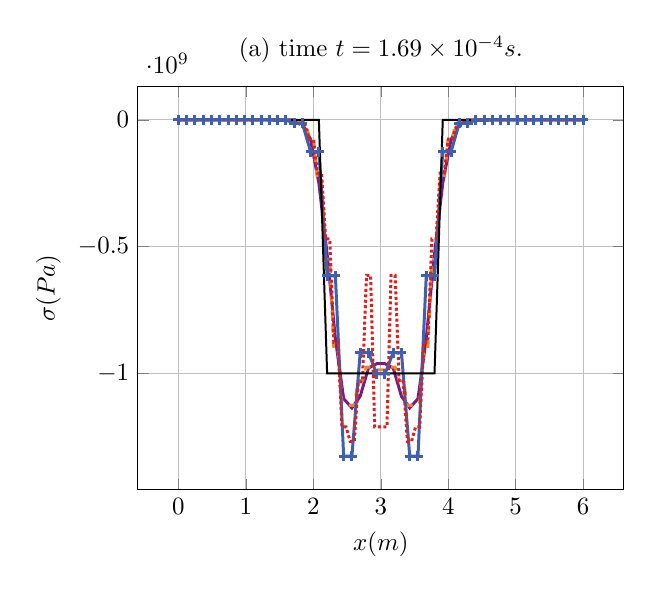
\begin{tikzpicture}[scale=0.9]
\begin{axis}[xlabel=$x (m)$,ylabel=$\sigma (Pa)$,ymajorgrids=true,xmajorgrids=true,title={(a) time $t =1.69\times 10^{-4}s.$}]
\addplot[Purple,very thick,mark=none,solid] coordinates {(0.0,-9.62200780097e-08) (0.122448979592,-1.92440156019e-07) (0.244897959184,-9.62200780097e-08) (0.367346938776,0.0) (0.489795918367,9.62200780097e-08) (0.612244897959,-9.62200780097e-08) (0.734693877551,-1.92440156019e-07) (0.857142857143,-9.62200780097e-08) (0.979591836735,-9.62200780097e-08) (1.10204081633,0.0) (1.22448979592,9.62200780097e-08) (1.34693877551,-9.62200780097e-08) (1.4693877551,0.0) (1.59183673469,0.0) (1.71428571429,0.0) (1.83673469388,-15437652.4848) (1.95918367347,-78183137.9185) (2.08163265306,-249067223.585) (2.20408163265,-529536815.675) (2.32653061224,-862202048.46) (2.44897959184,-1099498863.41) (2.57142857143,-1135789315.44) (2.69387755102,-1090007223.73) (2.81632653061,-978780358.738) (2.9387755102,-961497360.562) (3.0612244898,-961497360.562) (3.18367346939,-978780358.738) (3.30612244898,-1090007223.73) (3.42857142857,-1135789315.44) (3.55102040816,-1099498863.41) (3.67346938776,-862202048.46) (3.79591836735,-529536815.675) (3.91836734694,-249067223.585) (4.04081632653,-78183137.9185) (4.16326530612,-15437652.4848) (4.28571428571,-3.85185988877e-23) (4.40816326531,-9.62200780097e-08) (4.5306122449,9.62200780097e-08) (4.65306122449,9.62200780097e-08) (4.77551020408,9.62200780097e-08) (4.89795918367,-2.88660234029e-07) (5.02040816327,-9.62200780097e-08) (5.14285714286,9.62200780097e-08) (5.26530612245,1.92440156019e-07) (5.38775510204,2.88660234029e-07) (5.51020408163,9.62200780097e-08) (5.63265306122,0.0) (5.75510204082,0.0) (5.87755102041,0.0) (6.0,-9.62200780097e-08) };
\addplot[Orange,very thick,mark=none,dashed] coordinates {(0.0,0.0) (0.0606060606061,0.0) (0.121212121212,9.52481580298e-08) (0.181818181818,9.52481580298e-08) (0.242424242424,9.52481580298e-08) (0.30303030303,9.52481580298e-08) (0.363636363636,0.0) (0.424242424242,0.0) (0.484848484848,-9.52481580298e-08) (0.545454545455,-9.52481580298e-08) (0.606060606061,-1.9049631606e-07) (0.666666666667,-1.9049631606e-07) (0.727272727273,0.0) (0.787878787879,0.0) (0.848484848485,0.0) (0.909090909091,0.0) (0.969696969697,-3.85185988877e-23) (1.0303030303,-3.85185988877e-23) (1.09090909091,-9.52481580298e-08) (1.15151515152,-9.52481580298e-08) (1.21212121212,9.52481580298e-08) (1.27272727273,9.52481580298e-08) (1.33333333333,9.52481580298e-08) (1.39393939394,9.52481580298e-08) (1.45454545455,-1.9049631606e-07) (1.51515151515,-1.9049631606e-07) (1.57575757576,1.9049631606e-07) (1.63636363636,1.9049631606e-07) (1.69696969697,0.0) (1.75757575758,0.0) (1.81818181818,-9533923.2537) (1.87878787879,-9533923.2537) (1.93939393939,-67166647.336) (2.0,-67166647.336) (2.06060606061,-239339979.822) (2.12121212121,-239339979.822) (2.18181818182,-549695480.518) (2.24242424242,-549695480.518) (2.30303030303,-900240202.504) (2.36363636364,-900240202.504) (2.42424242424,-1118552245.0) (2.48484848485,-1118552245.0) (2.54545454545,-1125362633.2) (2.60606060606,-1125362633.2) (2.66666666667,-1028724363.35) (2.72727272727,-1028724363.35) (2.78787878788,-975375246.836) (2.84848484848,-975375246.836) (2.90909090909,-986009278.185) (2.9696969697,-986009278.185) (3.0303030303,-986009278.185) (3.09090909091,-986009278.185) (3.15151515152,-975375246.836) (3.21212121212,-975375246.836) (3.27272727273,-1028724363.35) (3.33333333333,-1028724363.35) (3.39393939394,-1125362633.2) (3.45454545455,-1125362633.2) (3.51515151515,-1118552245.0) (3.57575757576,-1118552245.0) (3.63636363636,-900240202.504) (3.69696969697,-900240202.504) (3.75757575758,-549695480.518) (3.81818181818,-549695480.518) (3.87878787879,-239339979.822) (3.93939393939,-239339979.822) (4.0,-67166647.336) (4.06060606061,-67166647.336) (4.12121212121,-9533923.2537) (4.18181818182,-9533923.2537) (4.24242424242,9.52481580298e-08) (4.30303030303,9.52481580298e-08) (4.36363636364,-9.52481580298e-08) (4.42424242424,-9.52481580298e-08) (4.48484848485,0.0) (4.54545454545,0.0) (4.60606060606,0.0) (4.66666666667,0.0) (4.72727272727,0.0) (4.78787878788,0.0) (4.84848484848,0.0) (4.90909090909,0.0) (4.9696969697,0.0) (5.0303030303,0.0) (5.09090909091,0.0) (5.15151515152,0.0) (5.21212121212,0.0) (5.27272727273,0.0) (5.33333333333,0.0) (5.39393939394,0.0) (5.45454545455,0.0) (5.51515151515,0.0) (5.57575757576,0.0) (5.63636363636,0.0) (5.69696969697,0.0) (5.75757575758,0.0) (5.81818181818,0.0) (5.87878787879,0.0) (5.93939393939,9.52481580298e-08) (6.0,9.52481580298e-08) };
\addplot[Blue,very thick,mark=+,solid] coordinates {(0.0,-3.84880312039e-07) (0.122448979592,2.88660234029e-07) (0.244897959184,-5.77320468058e-07) (0.367346938776,2.88660234029e-07) (0.489795918367,-9.62200780097e-08) (0.612244897959,2.88660234029e-07) (0.734693877551,-4.3483336004) (0.857142857143,-4.34833340796) (0.979591836735,-560.668787915) (1.10204081633,-560.668788299) (1.22448979592,-29850.7439455) (1.34693877551,-29850.7439456) (1.4693877551,-846060.279927) (1.59183673469,-846060.279927) (1.71428571429,-13703737.6015) (1.83673469388,-13703737.6015) (1.95918367347,-126206739.753) (2.08163265306,-126206739.753) (2.20408163265,-614922268.389) (2.32653061224,-614922268.389) (2.44897959184,-1325731906.52) (2.57142857143,-1325731906.52) (2.69387755102,-917663590.795) (2.81632653061,-917663590.795) (2.9387755102,-1001790561.8) (3.0612244898,-1001790561.8) (3.18367346939,-917663590.795) (3.30612244898,-917663590.795) (3.42857142857,-1325731906.52) (3.55102040816,-1325731906.52) (3.67346938776,-614922268.389) (3.79591836735,-614922268.389) (3.91836734694,-126206739.753) (4.04081632653,-126206739.753) (4.16326530612,-13703737.6015) (4.28571428571,-13703737.6015) (4.40816326531,-846060.279927) (4.5306122449,-846060.279927) (4.65306122449,-29850.7439458) (4.77551020408,-29850.7439452) (4.89795918367,-560.668787818) (5.02040816327,-560.668788011) (5.14285714286,-4.34833331174) (5.26530612245,-4.34833340796) (5.38775510204,1.92440156019e-07) (5.51020408163,-9.62200780097e-08) (5.63265306122,1.92440156019e-07) (5.75510204082,-2.88660234029e-07) (5.87755102041,4.81100390048e-07) (6.0,-2.88660234029e-07) };
\addplot[Red,very thick,mark=none,densely dotted] coordinates {(0.0,0.0) (0.0606060606061,0.0) (0.121212121212,9.52481580298e-08) (0.181818181818,9.52481580298e-08) (0.242424242424,-7.70371977755e-23) (0.30303030303,-7.70371977755e-23) (0.363636363636,-9.52481580298e-08) (0.424242424242,-9.52481580298e-08) (0.484848484848,-1.9049631606e-07) (0.545454545455,-1.9049631606e-07) (0.606060606061,1.9049631606e-07) (0.666666666667,1.9049631606e-07) (0.727272727273,-0.326493160065) (0.787878787879,-0.326493160065) (0.848484848485,-4.24441250957) (0.909090909091,-4.24441250957) (0.969696969697,-75.0667952395) (1.0303030303,-75.0667952395) (1.09090909091,-676.110516968) (1.15151515152,-676.110516968) (1.21212121212,-6409.50756423) (1.27272727273,-6409.50756423) (1.33333333333,-42608.4474487) (1.39393939394,-42608.4474487) (1.45454545455,-271096.202803) (1.51515151515,-271096.202803) (1.57575757576,-1361323.47494) (1.63636363636,-1361323.47494) (1.69696969697,-6186277.73843) (1.75757575758,-6186277.73843) (1.81818181818,-23394049.9045) (1.87878787879,-23394049.9045) (1.93939393939,-76154273.8888) (2.0,-76154273.8888) (2.06060606061,-210327688.316) (2.12121212121,-210327688.316) (2.18181818182,-469773248.386) (2.24242424242,-469773248.386) (2.30303030303,-877374801.132) (2.36363636364,-877374801.132) (2.42424242424,-1211041212.86) (2.48484848485,-1211041212.86) (2.54545454545,-1267995558.57) (2.60606060606,-1267995558.57) (2.66666666667,-1032834595.27) (2.72727272727,-1032834595.27) (2.78787878788,-612908579.142) (2.84848484848,-612908579.142) (2.90909090909,-1210327521.41) (2.9696969697,-1210327521.41) (3.0303030303,-1210327521.41) (3.09090909091,-1210327521.41) (3.15151515152,-612908579.142) (3.21212121212,-612908579.142) (3.27272727273,-1032834595.27) (3.33333333333,-1032834595.27) (3.39393939394,-1267995558.57) (3.45454545455,-1267995558.57) (3.51515151515,-1211041212.86) (3.57575757576,-1211041212.86) (3.63636363636,-877374801.132) (3.69696969697,-877374801.132) (3.75757575758,-469773248.386) (3.81818181818,-469773248.386) (3.87878787879,-210327688.316) (3.93939393939,-210327688.316) (4.0,-76154273.8888) (4.06060606061,-76154273.8888) (4.12121212121,-23394049.9045) (4.18181818182,-23394049.9045) (4.24242424242,-6186277.73843) (4.30303030303,-6186277.73843) (4.36363636364,-1361323.47494) (4.42424242424,-1361323.47494) (4.48484848485,-271096.202803) (4.54545454545,-271096.202803) (4.60606060606,-42608.4474489) (4.66666666667,-42608.4474489) (4.72727272727,-6409.50756433) (4.78787878788,-6409.50756433) (4.84848484848,-676.110516873) (4.90909090909,-676.110516873) (4.9696969697,-75.0667953347) (5.0303030303,-75.0667953347) (5.09090909091,-4.24441231907) (5.15151515152,-4.24441231907) (5.21212121212,-0.326493255313) (5.27272727273,-0.326493255313) (5.33333333333,0.0) (5.39393939394,0.0) (5.45454545455,0.0) (5.51515151515,0.0) (5.57575757576,0.0) (5.63636363636,0.0) (5.69696969697,0.0) (5.75757575758,0.0) (5.81818181818,0.0) (5.87878787879,0.0) (5.93939393939,0.0) (6.0,0.0) };
\addplot[black,thick] coordinates {(0.0,-0.0) (0.122448979592,-0.0) (0.244897959184,-0.0) (0.367346938776,-0.0) (0.489795918367,-0.0) (0.612244897959,-0.0) (0.734693877551,-0.0) (0.857142857143,-0.0) (0.979591836735,-0.0) (1.10204081633,-0.0) (1.22448979592,-0.0) (1.34693877551,-0.0) (1.4693877551,-0.0) (1.59183673469,-0.0) (1.71428571429,-0.0) (1.83673469388,-0.0) (1.95918367347,-0.0) (2.08163265306,-0.0) (2.20408163265,-1000000000.0) (2.32653061224,-1000000000.0) (2.44897959184,-1000000000.0) (2.57142857143,-1000000000.0) (2.69387755102,-1000000000.0) (2.81632653061,-1000000000.0) (2.9387755102,-1000000000.0) (3.0612244898,-1000000000.0) (3.18367346939,-1000000000.0) (3.30612244898,-1000000000.0) (3.42857142857,-1000000000.0) (3.55102040816,-1000000000.0) (3.67346938776,-1000000000.0) (3.79591836735,-1000000000.0) (3.91836734694,-0.0) (4.04081632653,-0.0) (4.16326530612,-0.0) (4.28571428571,-0.0) (4.40816326531,-0.0) (4.5306122449,-0.0) (4.65306122449,-0.0) (4.77551020408,-0.0) (4.89795918367,-0.0) (5.02040816327,-0.0) (5.14285714286,-0.0) (5.26530612245,-0.0) (5.38775510204,-0.0) (5.51020408163,-0.0) (5.63265306122,-0.0) (5.75510204082,-0.0) (5.87755102041,-0.0) (6.0,-0.0) };
%\legend{USL 1ppc,USL 2ppc,USF 1ppc,USF 2ppc}
\end{axis}
\end{tikzpicture}
 \phantomsubcaption \label{subfig:US_diffusion_10}}
  {\definecolor{Purple}{RGB}{120,28,129}
\definecolor{Orange}{RGB}{231,133,50}
\definecolor{Blue}{RGB}{63,96,174}
\definecolor{Red}{RGB}{217,33,32}
\definecolor{Duck}{RGB}{83,158,182}
\definecolor{Green}{RGB}{109,179,136}
\definecolor{Yellow}{RGB}{202,184,67}
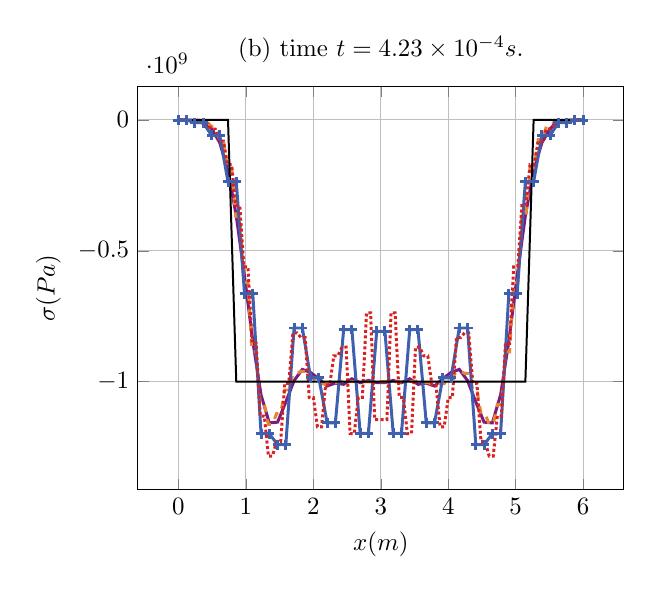
\begin{tikzpicture}[scale=0.9]
\begin{axis}[xlabel=$x (m)$,ylabel=$\sigma (Pa)$,ymajorgrids=true,xmajorgrids=true,title={(b) time $t= 4.23\times 10^{-4}s.$}]
\addplot[Purple,very thick,mark=none,solid] coordinates {(0.0,-39934.2174897) (0.122448979592,-406302.064953) (0.244897959184,-2420460.88495) (0.367346938776,-10136844.8366) (0.489795918367,-33063216.5915) (0.612244897959,-87547121.3685) (0.734693877551,-194171704.565) (0.857142857143,-366493404.576) (0.979591836735,-596875114.898) (1.10204081633,-845116689.368) (1.22448979592,-1050481005.19) (1.34693877551,-1157297307.0) (1.4693877551,-1154376682.02) (1.59183673469,-1077374033.62) (1.71428571429,-995689036.388) (1.83673469388,-952936697.469) (1.95918367347,-964832377.273) (2.08163265306,-988568067.368) (2.20408163265,-1016260759.09) (2.32653061224,-1005179173.62) (2.44897959184,-1009892551.13) (2.57142857143,-988773783.034) (2.69387755102,-1003829596.99) (2.81632653061,-995025027.704) (2.9387755102,-1003213108.71) (3.0612244898,-1003213108.71) (3.18367346939,-995025027.704) (3.30612244898,-1003829596.99) (3.42857142857,-988773783.034) (3.55102040816,-1009892551.13) (3.67346938776,-1005179173.62) (3.79591836735,-1016260759.09) (3.91836734694,-988568067.368) (4.04081632653,-964832377.273) (4.16326530612,-952936697.469) (4.28571428571,-995689036.388) (4.40816326531,-1077374033.62) (4.5306122449,-1154376682.02) (4.65306122449,-1157297307.0) (4.77551020408,-1050481005.19) (4.89795918367,-845116689.368) (5.02040816327,-596875114.898) (5.14285714286,-366493404.576) (5.26530612245,-194171704.565) (5.38775510204,-87547121.3685) (5.51020408163,-33063216.5915) (5.63265306122,-10136844.8366) (5.75510204082,-2420460.88495) (5.87755102041,-406302.064953) (6.0,-39934.2174897) };
\addplot[Orange,very thick,mark=none,dashed] coordinates {(0.0,-10429.0753611) (0.0606060606061,-10429.0753611) (0.121212121212,-161982.808053) (0.181818181818,-161982.808053) (0.242424242424,-1267409.75703) (0.30303030303,-1267409.75703) (0.363636363636,-6575307.60772) (0.424242424242,-6575307.60772) (0.484848484848,-25213047.7874) (0.545454545455,-25213047.7874) (0.606060606061,-75630068.1866) (0.666666666667,-75630068.1866) (0.727272727273,-183565723.323) (0.787878787879,-183565723.323) (0.848484848485,-368376215.18) (0.909090909091,-368376215.18) (0.969696969697,-620238104.743) (1.0303030303,-620238104.743) (1.09090909091,-886041263.042) (1.15151515152,-886041263.042) (1.21212121212,-1086232263.3) (1.27272727273,-1086232263.3) (1.33333333333,-1162610811.08) (1.39393939394,-1162610811.08) (1.45454545455,-1121800356.23) (1.51515151515,-1121800356.23) (1.57575757576,-1031608883.18) (1.63636363636,-1031608883.18) (1.69696969697,-967968470.151) (1.75757575758,-967968470.151) (1.81818181818,-960540680.349) (1.87878787879,-960540680.349) (1.93939393939,-986227377.719) (2.0,-986227377.719) (2.06060606061,-1007602191.25) (2.12121212121,-1007602191.25) (2.18181818182,-1009726046.8) (2.24242424242,-1009726046.8) (2.30303030303,-1002072997.71) (2.36363636364,-1002072997.71) (2.42424242424,-997465464.463) (2.48484848485,-997465464.463) (2.54545454545,-998318352.653) (2.60606060606,-998318352.653) (2.66666666667,-1000280134.99) (2.72727272727,-1000280134.99) (2.78787878788,-1000550813.71) (2.84848484848,-1000550813.71) (2.90909090909,-999915604.91) (2.9696969697,-999915604.91) (3.0303030303,-999915604.91) (3.09090909091,-999915604.91) (3.15151515152,-1000550813.71) (3.21212121212,-1000550813.71) (3.27272727273,-1000280134.99) (3.33333333333,-1000280134.99) (3.39393939394,-998318352.653) (3.45454545455,-998318352.653) (3.51515151515,-997465464.463) (3.57575757576,-997465464.463) (3.63636363636,-1002072997.71) (3.69696969697,-1002072997.71) (3.75757575758,-1009726046.8) (3.81818181818,-1009726046.8) (3.87878787879,-1007602191.25) (3.93939393939,-1007602191.25) (4.0,-986227377.719) (4.06060606061,-986227377.719) (4.12121212121,-960540680.349) (4.18181818182,-960540680.349) (4.24242424242,-967968470.151) (4.30303030303,-967968470.151) (4.36363636364,-1031608883.18) (4.42424242424,-1031608883.18) (4.48484848485,-1121800356.23) (4.54545454545,-1121800356.23) (4.60606060606,-1162610811.08) (4.66666666667,-1162610811.08) (4.72727272727,-1086232263.3) (4.78787878788,-1086232263.3) (4.84848484848,-886041263.042) (4.90909090909,-886041263.042) (4.9696969697,-620238104.743) (5.0303030303,-620238104.743) (5.09090909091,-368376215.18) (5.15151515152,-368376215.18) (5.21212121212,-183565723.323) (5.27272727273,-183565723.323) (5.33333333333,-75630068.1866) (5.39393939394,-75630068.1866) (5.45454545455,-25213047.7874) (5.51515151515,-25213047.7874) (5.57575757576,-6575307.60772) (5.63636363636,-6575307.60772) (5.69696969697,-1267409.75703) (5.75757575758,-1267409.75703) (5.81818181818,-161982.808054) (5.87878787879,-161982.808054) (5.93939393939,-10429.0753609) (6.0,-10429.0753609) };
\addplot[Blue,very thick,mark=+,solid] coordinates {(0.0,-1333876.13913) (0.122448979592,-1333876.13913) (0.244897959184,-10769880.3244) (0.367346938776,-10769880.3244) (0.489795918367,-59004320.4619) (0.612244897959,-59004320.4619) (0.734693877551,-236932522.32) (0.857142857143,-236932522.32) (0.979591836735,-663853517.052) (1.10204081633,-663853517.052) (1.22448979592,-1198320286.6) (1.34693877551,-1198320286.6) (1.4693877551,-1240363116.33) (1.59183673469,-1240363116.33) (1.71428571429,-794840746.96) (1.83673469388,-794840746.96) (1.95918367347,-985342724.542) (2.08163265306,-985342724.542) (2.20408163265,-1157175976.76) (2.32653061224,-1157175976.76) (2.44897959184,-800603512.041) (2.57142857143,-800603512.041) (2.69387755102,-1197082213.94) (2.81632653061,-1197082213.94) (2.9387755102,-808054803.925) (3.0612244898,-808054803.925) (3.18367346939,-1197082213.94) (3.30612244898,-1197082213.94) (3.42857142857,-800603512.041) (3.55102040816,-800603512.041) (3.67346938776,-1157175976.76) (3.79591836735,-1157175976.76) (3.91836734694,-985342724.542) (4.04081632653,-985342724.542) (4.16326530612,-794840746.96) (4.28571428571,-794840746.96) (4.40816326531,-1240363116.33) (4.5306122449,-1240363116.33) (4.65306122449,-1198320286.6) (4.77551020408,-1198320286.6) (4.89795918367,-663853517.052) (5.02040816327,-663853517.052) (5.14285714286,-236932522.32) (5.26530612245,-236932522.32) (5.38775510204,-59004320.4619) (5.51020408163,-59004320.4619) (5.63265306122,-10769880.3244) (5.75510204082,-10769880.3244) (5.87755102041,-1333876.13913) (6.0,-1333876.13913) };
\addplot[Red,very thick,mark=none,densely dotted] coordinates {(0.0,-388790.247817) (0.0606060606061,-388790.247817) (0.121212121212,-1698682.9889) (0.181818181818,-1698682.9889) (0.242424242424,-5114933.57998) (0.30303030303,-5114933.57998) (0.363636363636,-13968295.6879) (0.424242424242,-13968295.6879) (0.484848484848,-35149039.2515) (0.545454545455,-35149039.2515) (0.606060606061,-81229883.7541) (0.666666666667,-81229883.7541) (0.727272727273,-171384180.27) (0.787878787879,-171384180.27) (0.848484848485,-327574181.976) (0.909090909091,-327574181.976) (0.969696969697,-561694256.942) (1.0303030303,-561694256.942) (1.09090909091,-853480052.942) (1.15151515152,-853480052.942) (1.21212121212,-1131013878.06) (1.27272727273,-1131013878.06) (1.33333333333,-1283904880.31) (1.39393939394,-1283904880.31) (1.45454545455,-1228113384.33) (1.51515151515,-1228113384.33) (1.57575757576,-1005886402.14) (1.63636363636,-1005886402.14) (1.69696969697,-813073422.486) (1.75757575758,-813073422.486) (1.81818181818,-831794248.479) (1.87878787879,-831794248.479) (1.93939393939,-1060904062.7) (2.0,-1060904062.7) (2.06060606061,-1172530924.96) (2.12121212121,-1172530924.96) (2.18181818182,-1012253190.13) (2.24242424242,-1012253190.13) (2.30303030303,-901341875.005) (2.36363636364,-901341875.005) (2.42424242424,-867929277.273) (2.48484848485,-867929277.273) (2.54545454545,-1197799550.43) (2.60606060606,-1197799550.43) (2.66666666667,-1059717228.71) (2.72727272727,-1059717228.71) (2.78787878788,-736963301.649) (2.84848484848,-736963301.649) (2.90909090909,-1144647192.83) (2.9696969697,-1144647192.83) (3.0303030303,-1144647192.83) (3.09090909091,-1144647192.83) (3.15151515152,-736963301.649) (3.21212121212,-736963301.649) (3.27272727273,-1059717228.71) (3.33333333333,-1059717228.71) (3.39393939394,-1197799550.43) (3.45454545455,-1197799550.43) (3.51515151515,-867929277.273) (3.57575757576,-867929277.273) (3.63636363636,-901341875.005) (3.69696969697,-901341875.005) (3.75757575758,-1012253190.13) (3.81818181818,-1012253190.13) (3.87878787879,-1172530924.96) (3.93939393939,-1172530924.96) (4.0,-1060904062.7) (4.06060606061,-1060904062.7) (4.12121212121,-831794248.479) (4.18181818182,-831794248.479) (4.24242424242,-813073422.486) (4.30303030303,-813073422.486) (4.36363636364,-1005886402.14) (4.42424242424,-1005886402.14) (4.48484848485,-1228113384.33) (4.54545454545,-1228113384.33) (4.60606060606,-1283904880.31) (4.66666666667,-1283904880.31) (4.72727272727,-1131013878.06) (4.78787878788,-1131013878.06) (4.84848484848,-853480052.942) (4.90909090909,-853480052.942) (4.9696969697,-561694256.942) (5.0303030303,-561694256.942) (5.09090909091,-327574181.976) (5.15151515152,-327574181.976) (5.21212121212,-171384180.27) (5.27272727273,-171384180.27) (5.33333333333,-81229883.7541) (5.39393939394,-81229883.7541) (5.45454545455,-35149039.2515) (5.51515151515,-35149039.2515) (5.57575757576,-13968295.6879) (5.63636363636,-13968295.6879) (5.69696969697,-5114933.57998) (5.75757575758,-5114933.57998) (5.81818181818,-1698682.9889) (5.87878787879,-1698682.9889) (5.93939393939,-388790.247817) (6.0,-388790.247817) };
\addplot[black,thick] coordinates {(0.0,-0.0) (0.122448979592,-0.0) (0.244897959184,-0.0) (0.367346938776,-0.0) (0.489795918367,-0.0) (0.612244897959,-0.0) (0.734693877551,-0.0) (0.857142857143,-1000000000.0) (0.979591836735,-1000000000.0) (1.10204081633,-1000000000.0) (1.22448979592,-1000000000.0) (1.34693877551,-1000000000.0) (1.4693877551,-1000000000.0) (1.59183673469,-1000000000.0) (1.71428571429,-1000000000.0) (1.83673469388,-1000000000.0) (1.95918367347,-1000000000.0) (2.08163265306,-1000000000.0) (2.20408163265,-1000000000.0) (2.32653061224,-1000000000.0) (2.44897959184,-1000000000.0) (2.57142857143,-1000000000.0) (2.69387755102,-1000000000.0) (2.81632653061,-1000000000.0) (2.9387755102,-1000000000.0) (3.0612244898,-1000000000.0) (3.18367346939,-1000000000.0) (3.30612244898,-1000000000.0) (3.42857142857,-1000000000.0) (3.55102040816,-1000000000.0) (3.67346938776,-1000000000.0) (3.79591836735,-1000000000.0) (3.91836734694,-1000000000.0) (4.04081632653,-1000000000.0) (4.16326530612,-1000000000.0) (4.28571428571,-1000000000.0) (4.40816326531,-1000000000.0) (4.5306122449,-1000000000.0) (4.65306122449,-1000000000.0) (4.77551020408,-1000000000.0) (4.89795918367,-1000000000.0) (5.02040816327,-1000000000.0) (5.14285714286,-1000000000.0) (5.26530612245,-0.0) (5.38775510204,-0.0) (5.51020408163,-0.0) (5.63265306122,-0.0) (5.75510204082,-0.0) (5.87755102041,-0.0) (6.0,-0.0) };
%\legend{USL 1ppc,USL 2ppc,USF 1ppc,USF 2ppc}
\end{axis}
\end{tikzpicture}
 \phantomsubcaption \label{subfig:US_diffusion_25}}\\
  {\definecolor{Purple}{RGB}{120,28,129}
\definecolor{Orange}{RGB}{231,133,50}
\definecolor{Blue}{RGB}{63,96,174}
\definecolor{Red}{RGB}{217,33,32}
\definecolor{Duck}{RGB}{83,158,182}
\definecolor{Green}{RGB}{109,179,136}
\definecolor{Yellow}{RGB}{202,184,67}
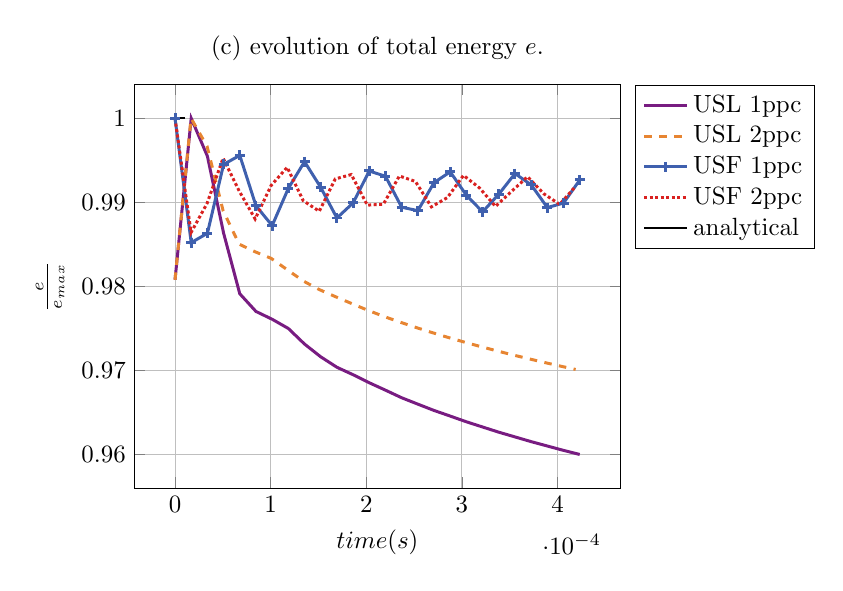
\begin{tikzpicture}[scale=0.9]
\begin{axis}[xlabel=$time (s)$,ylabel=$\frac{e}{e_{max}}$,ymajorgrids=true,xmajorgrids=true,title={(c) evolution of total energy $e$.},legend pos=outer north east]
\addplot[Purple,very thick,mark=none,solid] coordinates {(0.0,0.980776775206) (1.69272151355e-05,1.0) (3.38544302711e-05,0.995486386818) (5.07816454066e-05,0.986335480918) (6.77088605422e-05,0.979118179787) (8.46360756777e-05,0.977011836735) (0.000101563290813,0.976083552705) (0.000118490505949,0.974985958077) (0.000135417721084,0.973132007483) (0.00015234493622,0.971614043952) (0.000169272151355,0.970370597838) (0.000186199366491,0.969484052645) (0.000203126581626,0.968527091175) (0.000220053796762,0.967645365047) (0.000236981011898,0.966743210911) (0.000253908227033,0.965982183586) (0.000270835442169,0.965231974397) (0.000287762657304,0.964563191524) (0.00030468987244,0.96388114719) (0.000321617087575,0.963263530823) (0.000338544302711,0.962646353557) (0.000355471517846,0.962084695394) (0.000372398732982,0.961521764293) (0.000389325948117,0.961001071279) (0.000406253163253,0.960479919884) (0.000423180378389,0.959994795728) };
\addplot[Orange,very thick,mark=none,dashed] coordinates {(0.0,0.980776775206) (1.67562331645e-05,1.0) (3.3512466329e-05,0.996663809337) (5.02686994934e-05,0.98900666995) (6.70249326579e-05,0.985020324447) (8.37811658224e-05,0.984110580813) (0.000100537398987,0.983326915208) (0.000117293632151,0.981979184866) (0.000134049865316,0.980638155666) (0.00015080609848,0.979617302856) (0.000167562331645,0.978778886884) (0.000184318564809,0.977968446843) (0.000201074797974,0.977176694993) (0.000217831031138,0.976440965591) (0.000234587264303,0.975764557777) (0.000251343497467,0.975128766754) (0.000268099730632,0.974522184343) (0.000284855963796,0.973943735564) (0.000301612196961,0.973393220953) (0.000318368430125,0.972867749193) (0.00033512466329,0.972363947434) (0.000351880896454,0.971879647077) (0.000368637129618,0.971413467384) (0.000385393362783,0.970964070517) (0.000402149595947,0.97053007437) (0.000418905829112,0.970110254428) };
\addplot[Blue,very thick,mark=+,solid] coordinates {(0.0,1.0) (1.69272151355e-05,0.985202) (3.38544302711e-05,0.986310925125) (5.07816454066e-05,0.994507638064) (6.77088605422e-05,0.995579868604) (8.46360756777e-05,0.989584575004) (0.000101563290813,0.987225270569) (0.000118490505949,0.991657283729) (0.000135417721084,0.994836102021) (0.00015234493622,0.991773304725) (0.000169272151355,0.988131314159) (0.000186199366491,0.989928559949) (0.000203126581626,0.993725892454) (0.000220053796762,0.993092827557) (0.000236981011898,0.989412077079) (0.000253908227033,0.989007930164) (0.000270835442169,0.992337891088) (0.000287762657304,0.993619763816) (0.00030468987244,0.990831091012) (0.000321617087575,0.988860712515) (0.000338544302711,0.990967493415) (0.000355471517846,0.993415506334) (0.000372398732982,0.99207684926) (0.000389325948117,0.989372657972) (0.000406253163253,0.98991313843) (0.000423180378389,0.992654041387) };
\addplot[Red,very thick,mark=none,densely dotted] coordinates {(0.0,1.0) (1.67562331645e-05,0.9864025) (3.3512466329e-05,0.989873766211) (5.02686994934e-05,0.995255572924) (6.70249326579e-05,0.991355462516) (8.37811658224e-05,0.988011538229) (0.000100537398987,0.992011167376) (0.000117293632151,0.994160481387) (0.000134049865316,0.990189454195) (0.00015080609848,0.988933325063) (0.000167562331645,0.992779930372) (0.000184318564809,0.993300645038) (0.000201074797974,0.989660626012) (0.000217831031138,0.98976821642) (0.000234587264303,0.993129965182) (0.000251343497467,0.992481697852) (0.000268099730632,0.989459518699) (0.000284855963796,0.990567889043) (0.000301612196961,0.993200218105) (0.000318368430125,0.991710475421) (0.00033512466329,0.989506548964) (0.000351880896454,0.99129883371) (0.000368637129618,0.993048080156) (0.000385393362783,0.99103246412) (0.000402149595947,0.989751621209) (0.000418905829112,0.99191164529) };
\addplot[black,thick] coordinates {(0.,1.) (0.00001,1.)};
\legend{USL 1ppc,USL 2ppc,USF 1ppc,USF 2ppc,analytical}
\end{axis}
\end{tikzpicture}
 \phantomsubcaption \label{subfig:US_energies}}
  \caption{MPM solutions of the bars impact problem for various discretizations. (a)--(b) comparison of stress computed with USF and USL formulations and exact solutions (c) numerical total energy evolutions. Parameters: $CFL=0.7$ ; $v_0=\frac{1}{200}\sqrt{\frac{E}{\rho}}$.}
  \label{fig:US_diffusion}
\end{figure}
Figures \ref{fig:US_diffusion}\subref{subfig:US_diffusion_10} and \ref{fig:US_diffusion}\subref{subfig:US_diffusion_25} show that both USL and USF solutions oscillate after the passage of the elastic front. Those oscillations are much more significant in the USF solutions regardless of the number of particles used. Indeed, the noise in USL results quickly reduces so that the correct stress level is reached in the middle region of the bar. Moreover, even though the $1\: ppc$ and $2\: ppc$ discretizations provide different results (slightly different for USL), neither of them enables the removal of oscillations. Figure \ref{fig:US_diffusion}\subref{subfig:US_energies} shows, on the other hand, the evolutions of numerical total energies. Note that the total energy results from an MPM approximation of kinetic and strain energies, respectively defined as:
\begin{align}
  & e^{kin}=\frac{1}{2}\int_\Omega \rho \vect{v}\cdot\vect{v} \:d\Omega \approx \frac{1}{2}\sum_p m_p \vect{v}^p\cdot\vect{v}^p\\
& e^{strain}= \frac{1}{2}\int_\Omega \rho \tens{\bar{\sigma}}: \nablav \vect{v} \:d\Omega \approx \frac{1}{2}\sum_p m_p \tens{\bar{\sigma}}^p: \nablav \vect{v}^p
\end{align}
One can see that the USL formulation is more diffusive than the USF for this problem. These results differ from observations made in \cite{Bardenhagen_USF_USL}, in which no significant difference appears in energy plots for problems involving smooth solutions. At last, figure \ref{fig:US_velocities} compares the numerical velocities to the exact solution at various time steps. The same pattern than that observed for stresses is seen in figures \ref{fig:US_velocities}\subref{subfig:US_velo_10} and \ref{fig:US_velocities}\subref{subfig:US_velo_25} for velocities, namely, numerical oscillations in both USL and USF solutions with bigger picks in the USF ones. 

A notable numerical artifact that prevents the proper assessment of the velocity occurs at the middle of the bar. This issue is not due to the computation of internal forces since the symmetrical stress solutions plotted in figures \ref{fig:US_diffusion}\subref{subfig:US_diffusion_10} and \ref{fig:US_diffusion}\subref{subfig:US_diffusion_25}, combined to the discontinuous gradient of shape functions, yield zero internal forces at the central node of the computational grid (equation \eqref{eq:int_forces}). Furthermore, a skew-symmetric velocity solution leads, after the convective step, to a zero velocity at the central node, which is the correct solution (and never changes because of null internal forces). Hence, the error most likely comes from the back-mapping of fields from the grid to material points. 
\begin{figure}[h!]
  \centering
  {\definecolor{Purple}{RGB}{120,28,129}
\definecolor{Orange}{RGB}{231,133,50}
\definecolor{Blue}{RGB}{63,96,174}
\definecolor{Red}{RGB}{217,33,32}
\definecolor{Duck}{RGB}{83,158,182}
\definecolor{Green}{RGB}{109,179,136}
\definecolor{Yellow}{RGB}{202,184,67}
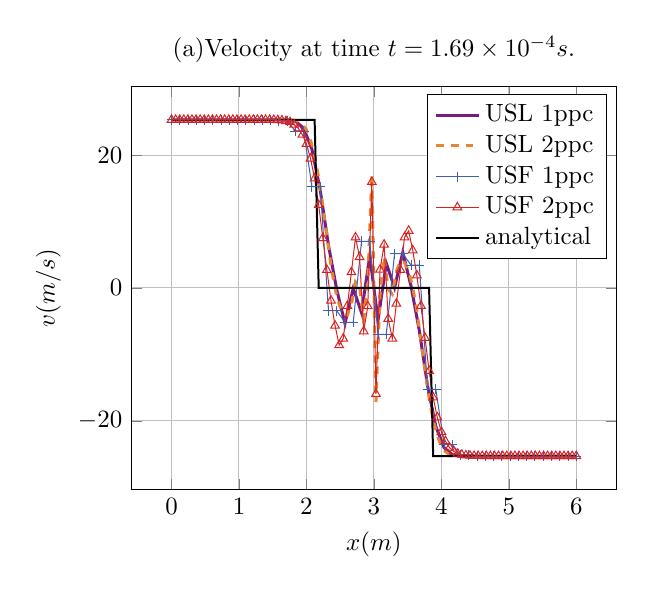
\begin{tikzpicture}[scale=0.9]
\begin{axis}[xlabel=$x (m)$,ylabel=$v (m/s)$,ymajorgrids=true,xmajorgrids=true,title={(a)Velocity at time $t=1.69\times 10^{-4}s.$}]
\addplot[Purple,very thick,mark=none,solid] coordinates {(0.0,25.3184841771) (0.122448979592,25.3184841771) (0.244897959184,25.3184841771) (0.367346938776,25.3184841771) (0.489795918367,25.3184841771) (0.612244897959,25.3184841771) (0.734693877551,25.3184841771) (0.857142857143,25.3184841771) (0.979591836735,25.3184841771) (1.10204081633,25.3184841771) (1.22448979592,25.3184841771) (1.34693877551,25.3184841771) (1.4693877551,25.3184841771) (1.59183673469,25.3184841771) (1.71428571429,25.3184841771) (1.83673469388,25.1149797615) (1.95918367347,24.0545424864) (2.08163265306,20.8743509476) (2.20408163265,14.7547033581) (2.32653061224,6.41598558277) (2.44897959184,-0.244456370035) (2.57142857143,-5.35821612759) (2.69387755102,-0.0619763112976) (2.81632653061,-3.709401685) (2.9387755102,4.8348853161) (3.0612244898,-4.8348853161) (3.18367346939,3.709401685) (3.30612244898,0.0619763112976) (3.42857142857,5.35821612759) (3.55102040816,0.244456370035) (3.67346938776,-6.41598558277) (3.79591836735,-14.7547033581) (3.91836734694,-20.8743509476) (4.04081632653,-24.0545424864) (4.16326530612,-25.1149797615) (4.28571428571,-25.3184841771) (4.40816326531,-25.3184841771) (4.5306122449,-25.3184841771) (4.65306122449,-25.3184841771) (4.77551020408,-25.3184841771) (4.89795918367,-25.3184841771) (5.02040816327,-25.3184841771) (5.14285714286,-25.3184841771) (5.26530612245,-25.3184841771) (5.38775510204,-25.3184841771) (5.51020408163,-25.3184841771) (5.63265306122,-25.3184841771) (5.75510204082,-25.3184841771) (5.87755102041,-25.3184841771) (6.0,-25.3184841771) };
\addplot[Orange,very thick,mark=none,dashed] coordinates {(0.0,25.3184841771) (0.0606060606061,25.3184841771) (0.121212121212,25.3184841771) (0.181818181818,25.3184841771) (0.242424242424,25.3184841771) (0.30303030303,25.3184841771) (0.363636363636,25.3184841771) (0.424242424242,25.3184841771) (0.484848484848,25.3184841771) (0.545454545455,25.3184841771) (0.606060606061,25.3184841771) (0.666666666667,25.3184841771) (0.727272727273,25.3184841771) (0.787878787879,25.3184841771) (0.848484848485,25.3184841771) (0.909090909091,25.3184841771) (0.969696969697,25.3184841771) (1.0303030303,25.3184841771) (1.09090909091,25.3184841771) (1.15151515152,25.3184841771) (1.21212121212,25.3184841771) (1.27272727273,25.3184841771) (1.33333333333,25.3184841771) (1.39393939394,25.3184841771) (1.45454545455,25.3184841771) (1.51515151515,25.3184841771) (1.57575757576,25.3184841771) (1.63636363636,25.3184841771) (1.69696969697,25.3184841771) (1.75757575758,25.3184841771) (1.81818181818,25.251933876) (1.87878787879,25.1188332739) (1.93939393939,24.6493504882) (2.0,23.8434855187) (2.06060606061,22.247450502) (2.12121212121,19.8612454379) (2.18181818182,16.5614104839) (2.24242424242,12.3479456399) (2.30303030303,7.94379399222) (2.36363636364,3.34895554082) (2.42424242424,-0.133198996542) (2.48484848485,-2.50266961986) (2.54545454545,-3.82041358095) (2.60606060606,-4.08643087983) (2.66666666667,-2.50894819569) (2.72727272727,0.91203447147) (2.78787878788,0.178185932665) (2.84848484848,-4.71049381211) (2.90909090909,0.963495780905) (2.9696969697,17.2001547117) (3.0303030303,-17.2001547117) (3.09090909091,-0.963495780905) (3.15151515152,4.7104938121) (3.21212121212,-0.178185932665) (3.27272727273,-0.91203447147) (3.33333333333,2.50894819569) (3.39393939394,4.08643087983) (3.45454545455,3.82041358095) (3.51515151515,2.50266961986) (3.57575757576,0.133198996542) (3.63636363636,-3.34895554082) (3.69696969697,-7.94379399222) (3.75757575758,-12.3479456399) (3.81818181818,-16.5614104839) (3.87878787879,-19.8612454379) (3.93939393939,-22.247450502) (4.0,-23.8434855187) (4.06060606061,-24.6493504882) (4.12121212121,-25.1188332739) (4.18181818182,-25.251933876) (4.24242424242,-25.3184841771) (4.30303030303,-25.3184841771) (4.36363636364,-25.3184841771) (4.42424242424,-25.3184841771) (4.48484848485,-25.3184841771) (4.54545454545,-25.3184841771) (4.60606060606,-25.3184841771) (4.66666666667,-25.3184841771) (4.72727272727,-25.3184841771) (4.78787878788,-25.3184841771) (4.84848484848,-25.3184841771) (4.90909090909,-25.3184841771) (4.9696969697,-25.3184841771) (5.0303030303,-25.3184841771) (5.09090909091,-25.3184841771) (5.15151515152,-25.3184841771) (5.21212121212,-25.3184841771) (5.27272727273,-25.3184841771) (5.33333333333,-25.3184841771) (5.39393939394,-25.3184841771) (5.45454545455,-25.3184841771) (5.51515151515,-25.3184841771) (5.57575757576,-25.3184841771) (5.63636363636,-25.3184841771) (5.69696969697,-25.3184841771) (5.75757575758,-25.3184841771) (5.81818181818,-25.3184841771) (5.87878787879,-25.3184841771) (5.93939393939,-25.3184841771) (6.0,-25.3184841771) };
\addplot[Blue,thin,mark=+,solid] coordinates {(0.0,25.3184841771) (0.122448979592,25.3184841771) (0.244897959184,25.3184841771) (0.367346938776,25.3184841771) (0.489795918367,25.3184841771) (0.612244897959,25.3184841386) (0.734693877551,25.3184841386) (0.857142857143,25.3184789327) (0.979591836735,25.3184789327) (1.10204081633,25.3181863193) (1.22448979592,25.3181863193) (1.34693877551,25.3093479957) (1.4693877551,25.3093479957) (1.59183673469,25.1550198372) (1.71428571429,25.1550198372) (1.83673469388,23.6026380028) (1.95918367347,23.6026380028) (2.08163265306,15.2761405323) (2.20408163265,15.2761405323) (2.32653061224,-3.42382560915) (2.44897959184,-3.42382560915) (2.57142857143,-5.17320665774) (2.69387755102,-5.17320665774) (2.81632653061,6.99898825925) (2.9387755102,6.99898825925) (3.0612244898,-6.99898825925) (3.18367346939,-6.99898825925) (3.30612244898,5.17320665774) (3.42857142857,5.17320665774) (3.55102040816,3.42382560915) (3.67346938776,3.42382560915) (3.79591836735,-15.2761405323) (3.91836734694,-15.2761405323) (4.04081632653,-23.6026380028) (4.16326530612,-23.6026380028) (4.28571428571,-25.1550198372) (4.40816326531,-25.1550198372) (4.5306122449,-25.3093479957) (4.65306122449,-25.3093479957) (4.77551020408,-25.3181863193) (4.89795918367,-25.3181863193) (5.02040816327,-25.3184789327) (5.14285714286,-25.3184789327) (5.26530612245,-25.3184841386) (5.38775510204,-25.3184841386) (5.51020408163,-25.3184841771) (5.63265306122,-25.3184841771) (5.75510204082,-25.3184841771) (5.87755102041,-25.3184841771) (6.0,-25.3184841771) };
\addplot[Red,thin,mark=triangle,solid] coordinates {(0.0,25.3184841771) (0.0606060606061,25.3184841771) (0.121212121212,25.3184841771) (0.181818181818,25.3184841771) (0.242424242424,25.3184841771) (0.30303030303,25.3184841771) (0.363636363636,25.3184841771) (0.424242424242,25.3184841771) (0.484848484848,25.3184841771) (0.545454545455,25.3184841771) (0.606060606061,25.3184841756) (0.666666666667,25.3184841728) (0.727272727273,25.3184841554) (0.787878787879,25.3184841236) (0.848484848485,25.3184837955) (0.909090909091,25.3184831711) (0.969696969697,25.3184803575) (1.0303030303,25.3184753545) (1.09090909091,25.3184471873) (1.15151515152,25.3183958557) (1.21212121212,25.3182145032) (1.27272727273,25.3179031296) (1.33333333333,25.3166920979) (1.39393939394,25.3145814079) (1.45454545455,25.3086270817) (1.51515151515,25.2988291195) (1.57575757576,25.2705514254) (1.63636363636,25.2237939997) (1.69696969697,25.1183204342) (1.75757575758,24.9541307292) (1.81818181818,24.5979538878) (1.87878787879,24.0497899101) (1.93939393939,23.076688448) (2.0,21.6786495014) (2.06060606061,19.4833431738) (2.12121212121,16.4907694654) (2.18181818182,12.4989085572) (2.24242424242,7.50776044936) (2.30303030303,2.70872378788) (2.36363636364,-1.89820142723) (2.42424242424,-5.67144294529) (2.48484848485,-8.61100076632) (2.54545454545,-7.62326403856) (2.60606060606,-2.70823276202) (2.66666666667,2.3712989244) (2.72727272727,7.61533102071) (2.78787878788,4.6503105848) (2.84848484848,-6.52376238331) (2.90909090909,-2.75347810625) (2.9696969697,15.961163416) (3.0303030303,-15.961163416) (3.09090909091,2.75347810625) (3.15151515152,6.52376238331) (3.21212121212,-4.6503105848) (3.27272727273,-7.61533102071) (3.33333333333,-2.3712989244) (3.39393939394,2.70823276202) (3.45454545455,7.62326403856) (3.51515151515,8.61100076632) (3.57575757576,5.67144294529) (3.63636363636,1.89820142723) (3.69696969697,-2.70872378788) (3.75757575758,-7.50776044936) (3.81818181818,-12.4989085572) (3.87878787879,-16.4907694654) (3.93939393939,-19.4833431738) (4.0,-21.6786495014) (4.06060606061,-23.076688448) (4.12121212121,-24.0497899101) (4.18181818182,-24.5979538878) (4.24242424242,-24.9541307292) (4.30303030303,-25.1183204342) (4.36363636364,-25.2237939997) (4.42424242424,-25.2705514254) (4.48484848485,-25.2988291195) (4.54545454545,-25.3086270817) (4.60606060606,-25.3145814079) (4.66666666667,-25.3166920979) (4.72727272727,-25.3179031296) (4.78787878788,-25.3182145032) (4.84848484848,-25.3183958557) (4.90909090909,-25.3184471873) (4.9696969697,-25.3184753545) (5.0303030303,-25.3184803575) (5.09090909091,-25.3184831711) (5.15151515152,-25.3184837955) (5.21212121212,-25.3184841236) (5.27272727273,-25.3184841554) (5.33333333333,-25.3184841728) (5.39393939394,-25.3184841756) (5.45454545455,-25.3184841771) (5.51515151515,-25.3184841771) (5.57575757576,-25.3184841771) (5.63636363636,-25.3184841771) (5.69696969697,-25.3184841771) (5.75757575758,-25.3184841771) (5.81818181818,-25.3184841771) (5.87878787879,-25.3184841771) (5.93939393939,-25.3184841771) (6.0,-25.3184841771) };
\addplot[black,thick,mark=none,solid] coordinates {(0.0,25.3184841771) (0.0606060606061,25.3184841771) (0.121212121212,25.3184841771) (0.181818181818,25.3184841771) (0.242424242424,25.3184841771) (0.30303030303,25.3184841771) (0.363636363636,25.3184841771) (0.424242424242,25.3184841771) (0.484848484848,25.3184841771) (0.545454545455,25.3184841771) (0.606060606061,25.3184841771) (0.666666666667,25.3184841771) (0.727272727273,25.3184841771) (0.787878787879,25.3184841771) (0.848484848485,25.3184841771) (0.909090909091,25.3184841771) (0.969696969697,25.3184841771) (1.0303030303,25.3184841771) (1.09090909091,25.3184841771) (1.15151515152,25.3184841771) (1.21212121212,25.3184841771) (1.27272727273,25.3184841771) (1.33333333333,25.3184841771) (1.39393939394,25.3184841771) (1.45454545455,25.3184841771) (1.51515151515,25.3184841771) (1.57575757576,25.3184841771) (1.63636363636,25.3184841771) (1.69696969697,25.3184841771) (1.75757575758,25.3184841771) (1.81818181818,25.3184841771) (1.87878787879,25.3184841771) (1.93939393939,25.3184841771) (2.0,25.3184841771) (2.06060606061,25.3184841771) (2.12121212121,25.3184841771) (2.18181818182,0.0) (2.24242424242,0.0) (2.30303030303,0.0) (2.36363636364,0.0) (2.42424242424,0.0) (2.48484848485,0.0) (2.54545454545,0.0) (2.60606060606,0.0) (2.66666666667,0.0) (2.72727272727,0.0) (2.78787878788,0.0) (2.84848484848,0.0) (2.90909090909,0.0) (2.9696969697,0.0) (3.0303030303,-0.0) (3.09090909091,-0.0) (3.15151515152,-0.0) (3.21212121212,-0.0) (3.27272727273,-0.0) (3.33333333333,-0.0) (3.39393939394,-0.0) (3.45454545455,-0.0) (3.51515151515,-0.0) (3.57575757576,-0.0) (3.63636363636,-0.0) (3.69696969697,-0.0) (3.75757575758,-0.0) (3.81818181818,-0.0) (3.87878787879,-25.3184841771) (3.93939393939,-25.3184841771) (4.0,-25.3184841771) (4.06060606061,-25.3184841771) (4.12121212121,-25.3184841771) (4.18181818182,-25.3184841771) (4.24242424242,-25.3184841771) (4.30303030303,-25.3184841771) (4.36363636364,-25.3184841771) (4.42424242424,-25.3184841771) (4.48484848485,-25.3184841771) (4.54545454545,-25.3184841771) (4.60606060606,-25.3184841771) (4.66666666667,-25.3184841771) (4.72727272727,-25.3184841771) (4.78787878788,-25.3184841771) (4.84848484848,-25.3184841771) (4.90909090909,-25.3184841771) (4.9696969697,-25.3184841771) (5.0303030303,-25.3184841771) (5.09090909091,-25.3184841771) (5.15151515152,-25.3184841771) (5.21212121212,-25.3184841771) (5.27272727273,-25.3184841771) (5.33333333333,-25.3184841771) (5.39393939394,-25.3184841771) (5.45454545455,-25.3184841771) (5.51515151515,-25.3184841771) (5.57575757576,-25.3184841771) (5.63636363636,-25.3184841771) (5.69696969697,-25.3184841771) (5.75757575758,-25.3184841771) (5.81818181818,-25.3184841771) (5.87878787879,-25.3184841771) (5.93939393939,-25.3184841771) (6.0,-25.3184841771) };
\legend{USL 1ppc,USL 2ppc,USF 1ppc,USF 2ppc,analytical}
\end{axis}
\end{tikzpicture}

%%% Local Variables: 
%%% mode: latex
%%% TeX-master: "../../mainManuscript"
%%% End:
\phantomsubcaption \label{subfig:US_velo_10}}
  {\definecolor{Purple}{RGB}{120,28,129}
\definecolor{Orange}{RGB}{231,133,50}
\definecolor{Blue}{RGB}{63,96,174}
\definecolor{Red}{RGB}{217,33,32}
\definecolor{Duck}{RGB}{83,158,182}
\definecolor{Green}{RGB}{109,179,136}
\definecolor{Yellow}{RGB}{202,184,67}
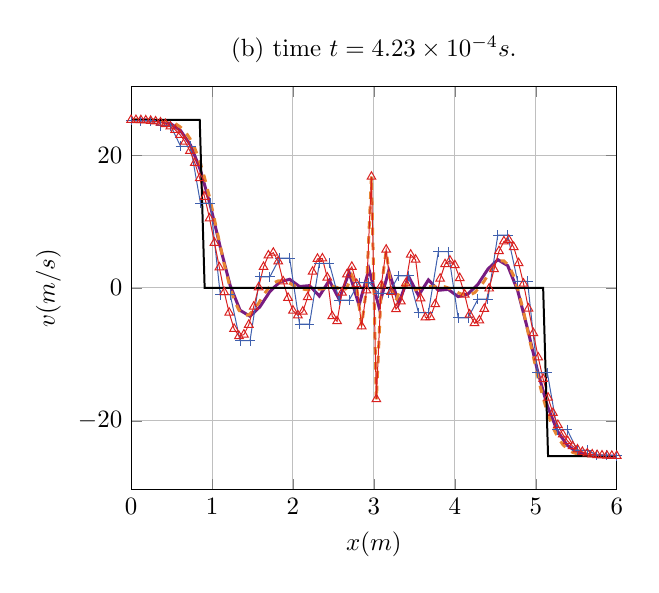
\begin{tikzpicture}[scale=0.9]
\begin{axis}[xlabel=$x (m)$,ylabel=$v (m/s)$,ymajorgrids=true,xmajorgrids=true,title={(b) time $t=4.23 \times 10^{-4}s$.},xmin=0.,xmax=6.]
\addplot[Purple,very thick,mark=none,solid] coordinates {(0.0,25.3179577559) (0.122448979592,25.3125244526) (0.244897959184,25.2804932478) (0.367346938776,25.1489907367) (0.489795918367,24.7341796044) (0.612244897959,23.6864809647) (0.734693877551,21.5118739395) (0.857142857143,17.7671095652) (0.979591836735,12.4121755247) (1.10204081633,6.14683940753) (1.22448979592,0.373716046882) (1.34693877551,-3.3616057723) (1.4693877551,-4.26176674269) (1.59183673469,-2.83406587609) (1.71428571429,-0.55562049587) (1.83673469388,0.901404345798) (1.95918367347,1.30403292578) (2.08163265306,0.214501074535) (2.20408163265,0.352209313776) (2.32653061224,-1.21718822558) (2.44897959184,1.14054029809) (2.57142857143,-1.72149525556) (2.69387755102,2.335373076) (2.81632653061,-2.59610029814) (2.9387755102,2.82071480229) (3.0612244898,-2.82071480229) (3.18367346939,2.59610029814) (3.30612244898,-2.335373076) (3.42857142857,1.72149525556) (3.55102040816,-1.14054029809) (3.67346938776,1.21718822558) (3.79591836735,-0.352209313776) (3.91836734694,-0.214501074535) (4.04081632653,-1.30403292578) (4.16326530612,-0.901404345798) (4.28571428571,0.55562049587) (4.40816326531,2.83406587609) (4.5306122449,4.26176674269) (4.65306122449,3.3616057723) (4.77551020408,-0.373716046882) (4.89795918367,-6.14683940753) (5.02040816327,-12.4121755247) (5.14285714286,-17.7671095652) (5.26530612245,-21.5118739395) (5.38775510204,-23.6864809647) (5.51020408163,-24.7341796044) (5.63265306122,-25.1489907367) (5.75510204082,-25.2804932478) (5.87755102041,-25.3125244526) (6.0,-25.3179577559) };
\addplot[Orange,very thick,mark=none,dashed] coordinates {(0.0,25.3184113784) (0.0606060606061,25.3182657812) (0.121212121212,25.3171343813) (0.181818181818,25.3150171787) (0.242424242424,25.3062460446) (0.30303030303,25.2908209787) (0.363636363636,25.2461773758) (0.424242424242,25.1723152357) (0.484848484848,25.0062868064) (0.545454545455,24.748092088) (0.606060606061,24.2720385643) (0.666666666667,23.5781262352) (0.727272727273,22.4951335769) (0.787878787879,21.0230605893) (0.848484848485,19.0428242456) (0.909090909091,16.5544245458) (0.969696969697,13.6460768618) (1.0303030303,10.3177811934) (1.09090909091,6.94923058708) (1.15151515152,3.54042504293) (1.21212121212,0.626561316633) (1.27272727273,-1.79236059183) (1.33333333333,-3.36301978655) (1.39393939394,-4.08541626753) (1.45454545455,-4.06554257142) (1.51515151515,-3.30339869822) (1.57575757576,-2.29577774705) (1.63636363636,-1.04267971791) (1.69696969697,-0.0393881478233) (1.75757575758,0.714096963215) (1.81818181818,1.07591385411) (1.87878787879,1.04606252486) (1.93939393939,0.832069940855) (2.0,0.433936102092) (2.06060606061,0.100491892604) (2.12121212121,-0.168262687611) (2.18181818182,-0.281962807299) (2.24242424242,-0.24060846646) (2.30303030303,-0.19473430746) (2.36363636364,-0.144340330301) (2.42424242424,0.0103021847971) (2.48484848485,0.269193237834) (2.54545454545,0.0743373654573) (2.60606060606,-0.574265432333) (2.66666666667,0.0252212025898) (2.72727272727,1.87279727022) (2.78787878788,-0.017779131944) (2.84848484848,-5.64650800392) (2.90909090909,-0.0160332856532) (2.9696969697,16.8736450228) (3.0303030303,-16.8736450228) (3.09090909091,0.0160332856532) (3.15151515152,5.64650800392) (3.21212121212,0.017779131944) (3.27272727273,-1.87279727022) (3.33333333333,-0.0252212025898) (3.39393939394,0.574265432333) (3.45454545455,-0.0743373654573) (3.51515151515,-0.269193237834) (3.57575757576,-0.0103021847971) (3.63636363636,0.144340330301) (3.69696969697,0.19473430746) (3.75757575758,0.24060846646) (3.81818181818,0.281962807299) (3.87878787879,0.168262687611) (3.93939393939,-0.100491892604) (4.0,-0.433936102092) (4.06060606061,-0.832069940855) (4.12121212121,-1.04606252486) (4.18181818182,-1.07591385411) (4.24242424242,-0.714096963215) (4.30303030303,0.0393881478233) (4.36363636364,1.04267971791) (4.42424242424,2.29577774705) (4.48484848485,3.30339869822) (4.54545454545,4.06554257142) (4.60606060606,4.08541626753) (4.66666666667,3.36301978655) (4.72727272727,1.79236059183) (4.78787878788,-0.626561316633) (4.84848484848,-3.54042504293) (4.90909090909,-6.94923058708) (4.9696969697,-10.3177811934) (5.0303030303,-13.6460768618) (5.09090909091,-16.5544245458) (5.15151515152,-19.0428242456) (5.21212121212,-21.0230605893) (5.27272727273,-22.4951335769) (5.33333333333,-23.5781262352) (5.39393939394,-24.2720385643) (5.45454545455,-24.748092088) (5.51515151515,-25.0062868064) (5.57575757576,-25.1723152357) (5.63636363636,-25.2461773758) (5.69696969697,-25.2908209787) (5.75757575758,-25.3062460446) (5.81818181818,-25.3150171787) (5.87878787879,-25.3171343813) (5.93939393939,-25.3182657812) (6.0,-25.3184113784) };
\addplot[Blue,thin,mark=+,solid] coordinates {(0.0,25.278692227) (0.122448979592,25.1632638972) (0.244897959184,25.1632638972) (0.367346938776,24.4134945697) (0.489795918367,24.4134945697) (0.612244897959,21.3339382893) (0.734693877551,21.3339382893) (0.857142857143,12.7864947989) (0.979591836735,12.7864947989) (1.10204081633,-1.00143026403) (1.22448979592,-1.00143026403) (1.34693877551,-7.94234859658) (1.4693877551,-7.94234859658) (1.59183673469,1.666718506) (1.71428571429,1.666718506) (1.83673469388,4.4983018773) (1.95918367347,4.4983018773) (2.08163265306,-5.4528024961) (2.20408163265,-5.4528024961) (2.32653061224,3.70951010765) (2.44897959184,3.70951010765) (2.57142857143,-1.8372342386) (2.69387755102,-1.8372342386) (2.81632653061,0.817767529336) (2.9387755102,0.817767529337) (3.0612244898,-0.817767529337) (3.18367346939,-0.817767529336) (3.30612244898,1.8372342386) (3.42857142857,1.8372342386) (3.55102040816,-3.70951010765) (3.67346938776,-3.70951010765) (3.79591836735,5.4528024961) (3.91836734694,5.4528024961) (4.04081632653,-4.4983018773) (4.16326530612,-4.4983018773) (4.28571428571,-1.666718506) (4.40816326531,-1.666718506) (4.5306122449,7.94234859658) (4.65306122449,7.94234859658) (4.77551020408,1.00143026403) (4.89795918367,1.00143026403) (5.02040816327,-12.7864947989) (5.14285714286,-12.7864947989) (5.26530612245,-21.3339382893) (5.38775510204,-21.3339382893) (5.51020408163,-24.4134945697) (5.63265306122,-24.4134945697) (5.75510204082,-25.1632638972) (5.87755102041,-25.1632638972) (6.0,-25.278692227) };
\addplot[Red,thin,mark=triangle,solid] coordinates {(0.0,25.2925663718) (0.0606060606061,25.2843839677) (0.121212121212,25.2634771526) (0.181818181818,25.2298459266) (0.242424242424,25.166861976) (0.30303030303,25.074525301) (0.363636363636,24.9151607465) (0.424242424242,24.6887683126) (0.484848484848,24.3234854983) (0.545454545455,23.8193123035) (0.606060606061,23.0610017936) (0.666666666667,22.0485539687) (0.727272727273,20.638560445) (0.787878787879,18.8310212227) (0.848484848485,16.5222107775) (0.909090909091,13.7121291096) (0.969696969697,10.4726131337) (1.0303030303,6.80366284984) (1.09090909091,3.09745596005) (1.15151515152,-0.646007535703) (1.21212121212,-3.7294710718) (1.27272727273,-6.15293464823) (1.33333333333,-7.25044901317) (1.39393939394,-7.02201416662) (1.45454545455,-5.54409239748) (1.51515151515,-2.81668370575) (1.57575757576,0.0833596298948) (1.63636363636,3.15603760945) (1.69696969697,4.89643176607) (1.75757575758,5.30454209975) (1.81818181818,4.00211543869) (1.87878787879,0.98915178291) (1.93939393939,-1.48619261955) (2.0,-3.42391776869) (2.06060606061,-4.1204907004) (2.12121212121,-3.57591141468) (2.18181818182,-1.3875328666) (2.24242424242,2.44464494385) (2.30303030303,4.38796385565) (2.36363636364,4.44242386881) (2.42424242424,1.55990936166) (2.48484848485,-4.2595796658) (2.54545454545,-5.01317341167) (2.60606060606,-0.700871875953) (2.66666666667,2.03314306079) (2.72727272727,3.18887139857) (2.78787878788,0.588067826574) (2.84848484848,-5.76926765519) (2.90909090909,-0.381330502781) (2.9696969697,16.7518792838) (3.0303030303,-16.7518792838) (3.09090909091,0.381330502781) (3.15151515152,5.76926765519) (3.21212121212,-0.588067826574) (3.27272727273,-3.18887139857) (3.33333333333,-2.03314306079) (3.39393939394,0.700871875953) (3.45454545455,5.01317341167) (3.51515151515,4.2595796658) (3.57575757576,-1.55990936166) (3.63636363636,-4.44242386881) (3.69696969697,-4.38796385565) (3.75757575758,-2.44464494385) (3.81818181818,1.3875328666) (3.87878787879,3.57591141468) (3.93939393939,4.1204907004) (4.0,3.42391776869) (4.06060606061,1.48619261955) (4.12121212121,-0.98915178291) (4.18181818182,-4.00211543869) (4.24242424242,-5.30454209975) (4.30303030303,-4.89643176607) (4.36363636364,-3.15603760945) (4.42424242424,-0.0833596298948) (4.48484848485,2.81668370575) (4.54545454545,5.54409239748) (4.60606060606,7.02201416662) (4.66666666667,7.25044901317) (4.72727272727,6.15293464823) (4.78787878788,3.7294710718) (4.84848484848,0.646007535703) (4.90909090909,-3.09745596005) (4.9696969697,-6.80366284984) (5.0303030303,-10.4726131337) (5.09090909091,-13.7121291096) (5.15151515152,-16.5222107775) (5.21212121212,-18.8310212227) (5.27272727273,-20.638560445) (5.33333333333,-22.0485539687) (5.39393939394,-23.0610017936) (5.45454545455,-23.8193123035) (5.51515151515,-24.3234854983) (5.57575757576,-24.6887683126) (5.63636363636,-24.9151607465) (5.69696969697,-25.074525301) (5.75757575758,-25.166861976) (5.81818181818,-25.2298459266) (5.87878787879,-25.2634771526) (5.93939393939,-25.2843839677) (6.0,-25.2925663718) };
\addplot[black,thick,mark=none,solid] coordinates {(0.0,25.3184841771) (0.0606060606061,25.3184841771) (0.121212121212,25.3184841771) (0.181818181818,25.3184841771) (0.242424242424,25.3184841771) (0.30303030303,25.3184841771) (0.363636363636,25.3184841771) (0.424242424242,25.3184841771) (0.484848484848,25.3184841771) (0.545454545455,25.3184841771) (0.606060606061,25.3184841771) (0.666666666667,25.3184841771) (0.727272727273,25.3184841771) (0.787878787879,25.3184841771) (0.848484848485,25.3184841771) (0.909090909091,0.0) (0.969696969697,0.0) (1.0303030303,0.0) (1.09090909091,0.0) (1.15151515152,0.0) (1.21212121212,0.0) (1.27272727273,0.0) (1.33333333333,0.0) (1.39393939394,0.0) (1.45454545455,0.0) (1.51515151515,0.0) (1.57575757576,0.0) (1.63636363636,0.0) (1.69696969697,0.0) (1.75757575758,0.0) (1.81818181818,0.0) (1.87878787879,0.0) (1.93939393939,0.0) (2.0,0.0) (2.06060606061,0.0) (2.12121212121,0.0) (2.18181818182,0.0) (2.24242424242,0.0) (2.30303030303,0.0) (2.36363636364,0.0) (2.42424242424,0.0) (2.48484848485,0.0) (2.54545454545,0.0) (2.60606060606,0.0) (2.66666666667,0.0) (2.72727272727,0.0) (2.78787878788,0.0) (2.84848484848,0.0) (2.90909090909,0.0) (2.9696969697,0.0) (3.0303030303,-0.0) (3.09090909091,-0.0) (3.15151515152,-0.0) (3.21212121212,-0.0) (3.27272727273,-0.0) (3.33333333333,-0.0) (3.39393939394,-0.0) (3.45454545455,-0.0) (3.51515151515,-0.0) (3.57575757576,-0.0) (3.63636363636,-0.0) (3.69696969697,-0.0) (3.75757575758,-0.0) (3.81818181818,-0.0) (3.87878787879,-0.0) (3.93939393939,-0.0) (4.0,-0.0) (4.06060606061,-0.0) (4.12121212121,-0.0) (4.18181818182,-0.0) (4.24242424242,-0.0) (4.30303030303,-0.0) (4.36363636364,-0.0) (4.42424242424,-0.0) (4.48484848485,-0.0) (4.54545454545,-0.0) (4.60606060606,-0.0) (4.66666666667,-0.0) (4.72727272727,-0.0) (4.78787878788,-0.0) (4.84848484848,-0.0) (4.90909090909,-0.0) (4.9696969697,-0.0) (5.0303030303,-0.0) (5.09090909091,-0.0) (5.15151515152,-25.3184841771) (5.21212121212,-25.3184841771) (5.27272727273,-25.3184841771) (5.33333333333,-25.3184841771) (5.39393939394,-25.3184841771) (5.45454545455,-25.3184841771) (5.51515151515,-25.3184841771) (5.57575757576,-25.3184841771) (5.63636363636,-25.3184841771) (5.69696969697,-25.3184841771) (5.75757575758,-25.3184841771) (5.81818181818,-25.3184841771) (5.87878787879,-25.3184841771) (5.93939393939,-25.3184841771) (6.0,-25.3184841771) };
%\legend{USL 1ppc,USL 2ppc,USF 1ppc,USF 2ppc,analytical}
\end{axis}
\end{tikzpicture}
%%% Local Variables:
%%% mode: latex
%%% TeX-master: "../../mainManuscript"
%%% End:
\phantomsubcaption \label{subfig:US_velo_25}}
  \caption{Comparison between exact, USF and USL velocities of the bars impact problem for various discretizations.}
  \label{fig:US_velocities}
\end{figure}

Since the back-mapping has been identified as being responsible for noise in the numerical solution in \cite{Mass_Flip}, the original projection from the grid to particles used in PIC may be introduced within the MPM. Instead of updating the material points velocities according to equation \eqref{eq:mp_velocity_update}, the Lagrangian deform with the grid and their velocities are computed after the solution of discrete equations as:
\begin{equation}
  \label{eq:PIC_Back-mapping}
  \vect{v}^{p,n+1}=\sum_{i=1}^{N_n} S_{ip}\vect{v}^{i,n+1}
\end{equation}
On the other hand, the particles positions are updated in the same way by using the nodal velocity \eqref{eq:position_update}. By doing so, the particles displacements exactly satisfy the relation $\vect{\dot{x}}^p=\vect{v}^p$, which is not the case in MPM. Moreover, the writing of the weak form \eqref{eq:mpm_discrete_weak} has been based on the definition \eqref{eq:PIC_Back-mapping} so that this projection seems more consistent than the update \eqref{eq:mp_velocity_update}. 
\begin{figure}[h!]
  \centering
  {\definecolor{Purple}{RGB}{120,28,129}
\definecolor{Orange}{RGB}{231,133,50}
\definecolor{Blue}{RGB}{63,96,174}
\definecolor{Red}{RGB}{217,33,32}
\definecolor{Duck}{RGB}{83,158,182}
\definecolor{Green}{RGB}{109,179,136}
\definecolor{Yellow}{RGB}{202,184,67}
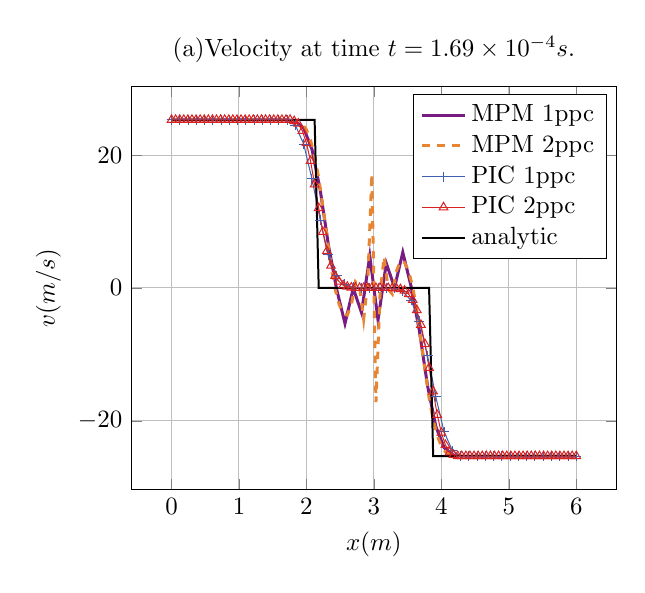
\begin{tikzpicture}[scale=0.9]
\begin{axis}[xlabel=$x (m)$,ylabel=$v (m/s)$,ymajorgrids=true,xmajorgrids=true,title={(a)Velocity at time $t=1.69\times 10^{-4}s.$}]
\addplot[Purple,very thick,mark=none,solid] coordinates {(0.0,25.3184841771) (0.122448979592,25.3184841771) (0.244897959184,25.3184841771) (0.367346938776,25.3184841771) (0.489795918367,25.3184841771) (0.612244897959,25.3184841771) (0.734693877551,25.3184841771) (0.857142857143,25.3184841771) (0.979591836735,25.3184841771) (1.10204081633,25.3184841771) (1.22448979592,25.3184841771) (1.34693877551,25.3184841771) (1.4693877551,25.3184841771) (1.59183673469,25.3184841771) (1.71428571429,25.3184841771) (1.83673469388,25.1149797615) (1.95918367347,24.0545424864) (2.08163265306,20.8743509476) (2.20408163265,14.7547033581) (2.32653061224,6.41598558277) (2.44897959184,-0.244456370035) (2.57142857143,-5.35821612759) (2.69387755102,-0.0619763112976) (2.81632653061,-3.709401685) (2.9387755102,4.8348853161) (3.0612244898,-4.8348853161) (3.18367346939,3.709401685) (3.30612244898,0.0619763112976) (3.42857142857,5.35821612759) (3.55102040816,0.244456370035) (3.67346938776,-6.41598558277) (3.79591836735,-14.7547033581) (3.91836734694,-20.8743509476) (4.04081632653,-24.0545424864) (4.16326530612,-25.1149797615) (4.28571428571,-25.3184841771) (4.40816326531,-25.3184841771) (4.5306122449,-25.3184841771) (4.65306122449,-25.3184841771) (4.77551020408,-25.3184841771) (4.89795918367,-25.3184841771) (5.02040816327,-25.3184841771) (5.14285714286,-25.3184841771) (5.26530612245,-25.3184841771) (5.38775510204,-25.3184841771) (5.51020408163,-25.3184841771) (5.63265306122,-25.3184841771) (5.75510204082,-25.3184841771) (5.87755102041,-25.3184841771) (6.0,-25.3184841771) };
\addplot[Orange,very thick,mark=none,dashed] coordinates {(0.0,25.3184841771) (0.0606060606061,25.3184841771) (0.121212121212,25.3184841771) (0.181818181818,25.3184841771) (0.242424242424,25.3184841771) (0.30303030303,25.3184841771) (0.363636363636,25.3184841771) (0.424242424242,25.3184841771) (0.484848484848,25.3184841771) (0.545454545455,25.3184841771) (0.606060606061,25.3184841771) (0.666666666667,25.3184841771) (0.727272727273,25.3184841771) (0.787878787879,25.3184841771) (0.848484848485,25.3184841771) (0.909090909091,25.3184841771) (0.969696969697,25.3184841771) (1.0303030303,25.3184841771) (1.09090909091,25.3184841771) (1.15151515152,25.3184841771) (1.21212121212,25.3184841771) (1.27272727273,25.3184841771) (1.33333333333,25.3184841771) (1.39393939394,25.3184841771) (1.45454545455,25.3184841771) (1.51515151515,25.3184841771) (1.57575757576,25.3184841771) (1.63636363636,25.3184841771) (1.69696969697,25.3184841771) (1.75757575758,25.3184841771) (1.81818181818,25.251933876) (1.87878787879,25.1188332739) (1.93939393939,24.6493504882) (2.0,23.8434855187) (2.06060606061,22.247450502) (2.12121212121,19.8612454379) (2.18181818182,16.5614104839) (2.24242424242,12.3479456399) (2.30303030303,7.94379399222) (2.36363636364,3.34895554082) (2.42424242424,-0.133198996542) (2.48484848485,-2.50266961986) (2.54545454545,-3.82041358095) (2.60606060606,-4.08643087983) (2.66666666667,-2.50894819569) (2.72727272727,0.91203447147) (2.78787878788,0.178185932665) (2.84848484848,-4.71049381211) (2.90909090909,0.963495780905) (2.9696969697,17.2001547117) (3.0303030303,-17.2001547117) (3.09090909091,-0.963495780905) (3.15151515152,4.7104938121) (3.21212121212,-0.178185932665) (3.27272727273,-0.91203447147) (3.33333333333,2.50894819569) (3.39393939394,4.08643087983) (3.45454545455,3.82041358095) (3.51515151515,2.50266961986) (3.57575757576,0.133198996542) (3.63636363636,-3.34895554082) (3.69696969697,-7.94379399222) (3.75757575758,-12.3479456399) (3.81818181818,-16.5614104839) (3.87878787879,-19.8612454379) (3.93939393939,-22.247450502) (4.0,-23.8434855187) (4.06060606061,-24.6493504882) (4.12121212121,-25.1188332739) (4.18181818182,-25.251933876) (4.24242424242,-25.3184841771) (4.30303030303,-25.3184841771) (4.36363636364,-25.3184841771) (4.42424242424,-25.3184841771) (4.48484848485,-25.3184841771) (4.54545454545,-25.3184841771) (4.60606060606,-25.3184841771) (4.66666666667,-25.3184841771) (4.72727272727,-25.3184841771) (4.78787878788,-25.3184841771) (4.84848484848,-25.3184841771) (4.90909090909,-25.3184841771) (4.9696969697,-25.3184841771) (5.0303030303,-25.3184841771) (5.09090909091,-25.3184841771) (5.15151515152,-25.3184841771) (5.21212121212,-25.3184841771) (5.27272727273,-25.3184841771) (5.33333333333,-25.3184841771) (5.39393939394,-25.3184841771) (5.45454545455,-25.3184841771) (5.51515151515,-25.3184841771) (5.57575757576,-25.3184841771) (5.63636363636,-25.3184841771) (5.69696969697,-25.3184841771) (5.75757575758,-25.3184841771) (5.81818181818,-25.3184841771) (5.87878787879,-25.3184841771) (5.93939393939,-25.3184841771) (6.0,-25.3184841771) };
\addplot[Blue,thin,mark=+,solid] coordinates {(0.0,25.3184841771) (0.122448979592,25.3184841771) (0.244897959184,25.3184841771) (0.367346938776,25.3184841771) (0.489795918367,25.3184841771) (0.612244897959,25.3184841771) (0.734693877551,25.3184841771) (0.857142857143,25.3184841771) (0.979591836735,25.3184841771) (1.10204081633,25.3184841771) (1.22448979592,25.3184841771) (1.34693877551,25.3184841771) (1.4693877551,25.3184841771) (1.59183673469,25.3184841771) (1.71428571429,25.3184841771) (1.83673469388,24.4761330084) (1.95918367347,21.6789610487) (2.08163265306,16.4171127559) (2.20408163265,10.2176854187) (2.32653061224,4.99697293397) (2.44897959184,1.87425322807) (2.57142857143,0.532987126345) (2.69387755102,0.0744368580376) (2.81632653061,0.0446687900239) (2.9387755102,-0.0367040274884) (3.0612244898,0.0367040274884) (3.18367346939,-0.0446687900239) (3.30612244898,-0.0744368580376) (3.42857142857,-0.532987126345) (3.55102040816,-1.87425322807) (3.67346938776,-4.99697293397) (3.79591836735,-10.2176854187) (3.91836734694,-16.4171127559) (4.04081632653,-21.6789610487) (4.16326530612,-24.4761330084) (4.28571428571,-25.3184841771) (4.40816326531,-25.3184841771) (4.5306122449,-25.3184841771) (4.65306122449,-25.3184841771) (4.77551020408,-25.3184841771) (4.89795918367,-25.3184841771) (5.02040816327,-25.3184841771) (5.14285714286,-25.3184841771) (5.26530612245,-25.3184841771) (5.38775510204,-25.3184841771) (5.51020408163,-25.3184841771) (5.63265306122,-25.3184841771) (5.75510204082,-25.3184841771) (5.87755102041,-25.3184841771) (6.0,-25.3184841771) };
\addplot[Red,thin,mark=triangle,solid] coordinates {(0.0,25.3184841771) (0.0606060606061,25.3184841771) (0.121212121212,25.3184841771) (0.181818181818,25.3184841771) (0.242424242424,25.3184841771) (0.30303030303,25.3184841771) (0.363636363636,25.3184841771) (0.424242424242,25.3184841771) (0.484848484848,25.3184841771) (0.545454545455,25.3184841771) (0.606060606061,25.3184841771) (0.666666666667,25.3184841771) (0.727272727273,25.3184841771) (0.787878787879,25.3184841771) (0.848484848485,25.3184841771) (0.909090909091,25.3184841771) (0.969696969697,25.3184841771) (1.0303030303,25.3184841771) (1.09090909091,25.3184841771) (1.15151515152,25.3184841771) (1.21212121212,25.3184841771) (1.27272727273,25.3184841771) (1.33333333333,25.3184841771) (1.39393939394,25.3184841771) (1.45454545455,25.3184841771) (1.51515151515,25.3184841771) (1.57575757576,25.3184841771) (1.63636363636,25.3184841771) (1.69696969697,25.3184841771) (1.75757575758,25.3184841771) (1.81818181818,25.1281304409) (1.87878787879,24.7474229685) (1.93939393939,23.6387415979) (2.0,21.8020863292) (2.06060606061,19.1201129846) (2.12121212121,15.5928215642) (2.18181818182,12.0349431808) (2.24242424242,8.44647783432) (2.30303030303,5.5505820269) (2.36363636364,3.3472557585) (2.42424242424,1.81296030454) (2.48484848485,0.947695665037) (2.54545454545,0.405594826726) (2.60606060606,0.186657789609) (2.66666666667,0.0594742699364) (2.72727272727,0.0240442677077) (2.78787878788,0.00485504304949) (2.84848484848,0.00190659596188) (2.90909090909,0.000324279313551) (2.9696969697,0.000108093104517) (3.0303030303,-0.000108093104518) (3.09090909091,-0.000324279313554) (3.15151515152,-0.00190659596188) (3.21212121212,-0.0048550430495) (3.27272727273,-0.0240442677077) (3.33333333333,-0.0594742699364) (3.39393939394,-0.186657789609) (3.45454545455,-0.405594826726) (3.51515151515,-0.947695665037) (3.57575757576,-1.81296030454) (3.63636363636,-3.3472557585) (3.69696969697,-5.5505820269) (3.75757575758,-8.44647783432) (3.81818181818,-12.0349431808) (3.87878787879,-15.5928215642) (3.93939393939,-19.1201129846) (4.0,-21.8020863292) (4.06060606061,-23.6387415979) (4.12121212121,-24.7474229685) (4.18181818182,-25.1281304409) (4.24242424242,-25.3184841771) (4.30303030303,-25.3184841771) (4.36363636364,-25.3184841771) (4.42424242424,-25.3184841771) (4.48484848485,-25.3184841771) (4.54545454545,-25.3184841771) (4.60606060606,-25.3184841771) (4.66666666667,-25.3184841771) (4.72727272727,-25.3184841771) (4.78787878788,-25.3184841771) (4.84848484848,-25.3184841771) (4.90909090909,-25.3184841771) (4.9696969697,-25.3184841771) (5.0303030303,-25.3184841771) (5.09090909091,-25.3184841771) (5.15151515152,-25.3184841771) (5.21212121212,-25.3184841771) (5.27272727273,-25.3184841771) (5.33333333333,-25.3184841771) (5.39393939394,-25.3184841771) (5.45454545455,-25.3184841771) (5.51515151515,-25.3184841771) (5.57575757576,-25.3184841771) (5.63636363636,-25.3184841771) (5.69696969697,-25.3184841771) (5.75757575758,-25.3184841771) (5.81818181818,-25.3184841771) (5.87878787879,-25.3184841771) (5.93939393939,-25.3184841771) (6.0,-25.3184841771) };
\addplot[black,thick,mark=none,solid] coordinates {(0.0,25.3184841771) (0.0606060606061,25.3184841771) (0.121212121212,25.3184841771) (0.181818181818,25.3184841771) (0.242424242424,25.3184841771) (0.30303030303,25.3184841771) (0.363636363636,25.3184841771) (0.424242424242,25.3184841771) (0.484848484848,25.3184841771) (0.545454545455,25.3184841771) (0.606060606061,25.3184841771) (0.666666666667,25.3184841771) (0.727272727273,25.3184841771) (0.787878787879,25.3184841771) (0.848484848485,25.3184841771) (0.909090909091,25.3184841771) (0.969696969697,25.3184841771) (1.0303030303,25.3184841771) (1.09090909091,25.3184841771) (1.15151515152,25.3184841771) (1.21212121212,25.3184841771) (1.27272727273,25.3184841771) (1.33333333333,25.3184841771) (1.39393939394,25.3184841771) (1.45454545455,25.3184841771) (1.51515151515,25.3184841771) (1.57575757576,25.3184841771) (1.63636363636,25.3184841771) (1.69696969697,25.3184841771) (1.75757575758,25.3184841771) (1.81818181818,25.3184841771) (1.87878787879,25.3184841771) (1.93939393939,25.3184841771) (2.0,25.3184841771) (2.06060606061,25.3184841771) (2.12121212121,25.3184841771) (2.18181818182,0.0) (2.24242424242,0.0) (2.30303030303,0.0) (2.36363636364,0.0) (2.42424242424,0.0) (2.48484848485,0.0) (2.54545454545,0.0) (2.60606060606,0.0) (2.66666666667,0.0) (2.72727272727,0.0) (2.78787878788,0.0) (2.84848484848,0.0) (2.90909090909,0.0) (2.9696969697,0.0) (3.0303030303,-0.0) (3.09090909091,-0.0) (3.15151515152,-0.0) (3.21212121212,-0.0) (3.27272727273,-0.0) (3.33333333333,-0.0) (3.39393939394,-0.0) (3.45454545455,-0.0) (3.51515151515,-0.0) (3.57575757576,-0.0) (3.63636363636,-0.0) (3.69696969697,-0.0) (3.75757575758,-0.0) (3.81818181818,-0.0) (3.87878787879,-25.3184841771) (3.93939393939,-25.3184841771) (4.0,-25.3184841771) (4.06060606061,-25.3184841771) (4.12121212121,-25.3184841771) (4.18181818182,-25.3184841771) (4.24242424242,-25.3184841771) (4.30303030303,-25.3184841771) (4.36363636364,-25.3184841771) (4.42424242424,-25.3184841771) (4.48484848485,-25.3184841771) (4.54545454545,-25.3184841771) (4.60606060606,-25.3184841771) (4.66666666667,-25.3184841771) (4.72727272727,-25.3184841771) (4.78787878788,-25.3184841771) (4.84848484848,-25.3184841771) (4.90909090909,-25.3184841771) (4.9696969697,-25.3184841771) (5.0303030303,-25.3184841771) (5.09090909091,-25.3184841771) (5.15151515152,-25.3184841771) (5.21212121212,-25.3184841771) (5.27272727273,-25.3184841771) (5.33333333333,-25.3184841771) (5.39393939394,-25.3184841771) (5.45454545455,-25.3184841771) (5.51515151515,-25.3184841771) (5.57575757576,-25.3184841771) (5.63636363636,-25.3184841771) (5.69696969697,-25.3184841771) (5.75757575758,-25.3184841771) (5.81818181818,-25.3184841771) (5.87878787879,-25.3184841771) (5.93939393939,-25.3184841771) (6.0,-25.3184841771) };
\legend{MPM 1ppc,MPM 2ppc,PIC 1ppc,PIC 2ppc,analytic}
\end{axis}
\end{tikzpicture}
%%% Local Variables: 
%%% mode: latex
%%% TeX-master: "../../mainManuscript"
%%% End:
\phantomsubcaption \label{subfig:MPM_velo_10}}
  {\definecolor{Purple}{RGB}{120,28,129}
\definecolor{Orange}{RGB}{231,133,50}
\definecolor{Blue}{RGB}{63,96,174}
\definecolor{Red}{RGB}{217,33,32}
\definecolor{Duck}{RGB}{83,158,182}
\definecolor{Green}{RGB}{109,179,136}
\definecolor{Yellow}{RGB}{202,184,67}
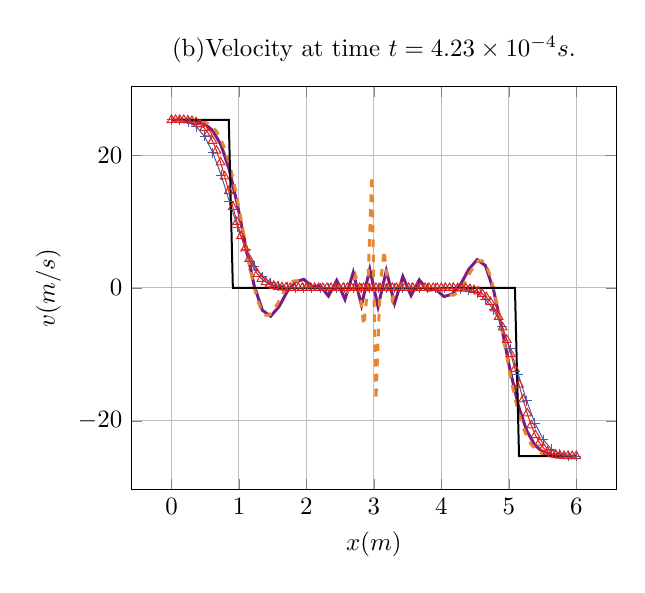
\begin{tikzpicture}[scale=0.9]
\begin{axis}[xlabel=$x (m)$,ylabel=$v (m/s)$,ymajorgrids=true,xmajorgrids=true,title={(b)Velocity at time $t=4.23\times 10^{-4}s.$}]
\addplot[Purple,very thick,mark=none,solid] coordinates {(0.0,25.3179577559) (0.122448979592,25.3125244526) (0.244897959184,25.2804932478) (0.367346938776,25.1489907367) (0.489795918367,24.7341796044) (0.612244897959,23.6864809647) (0.734693877551,21.5118739395) (0.857142857143,17.7671095652) (0.979591836735,12.4121755247) (1.10204081633,6.14683940753) (1.22448979592,0.373716046882) (1.34693877551,-3.3616057723) (1.4693877551,-4.26176674269) (1.59183673469,-2.83406587609) (1.71428571429,-0.55562049587) (1.83673469388,0.901404345798) (1.95918367347,1.30403292578) (2.08163265306,0.214501074535) (2.20408163265,0.352209313776) (2.32653061224,-1.21718822558) (2.44897959184,1.14054029809) (2.57142857143,-1.72149525556) (2.69387755102,2.335373076) (2.81632653061,-2.59610029814) (2.9387755102,2.82071480229) (3.0612244898,-2.82071480229) (3.18367346939,2.59610029814) (3.30612244898,-2.335373076) (3.42857142857,1.72149525556) (3.55102040816,-1.14054029809) (3.67346938776,1.21718822558) (3.79591836735,-0.352209313776) (3.91836734694,-0.214501074535) (4.04081632653,-1.30403292578) (4.16326530612,-0.901404345798) (4.28571428571,0.55562049587) (4.40816326531,2.83406587609) (4.5306122449,4.26176674269) (4.65306122449,3.3616057723) (4.77551020408,-0.373716046882) (4.89795918367,-6.14683940753) (5.02040816327,-12.4121755247) (5.14285714286,-17.7671095652) (5.26530612245,-21.5118739395) (5.38775510204,-23.6864809647) (5.51020408163,-24.7341796044) (5.63265306122,-25.1489907367) (5.75510204082,-25.2804932478) (5.87755102041,-25.3125244526) (6.0,-25.3179577559) };
\addplot[Orange,very thick,mark=none,dashed] coordinates {(0.0,25.3184113784) (0.0606060606061,25.3182657812) (0.121212121212,25.3171343813) (0.181818181818,25.3150171787) (0.242424242424,25.3062460446) (0.30303030303,25.2908209787) (0.363636363636,25.2461773758) (0.424242424242,25.1723152357) (0.484848484848,25.0062868064) (0.545454545455,24.748092088) (0.606060606061,24.2720385643) (0.666666666667,23.5781262352) (0.727272727273,22.4951335769) (0.787878787879,21.0230605893) (0.848484848485,19.0428242456) (0.909090909091,16.5544245458) (0.969696969697,13.6460768618) (1.0303030303,10.3177811934) (1.09090909091,6.94923058708) (1.15151515152,3.54042504293) (1.21212121212,0.626561316633) (1.27272727273,-1.79236059183) (1.33333333333,-3.36301978655) (1.39393939394,-4.08541626753) (1.45454545455,-4.06554257142) (1.51515151515,-3.30339869822) (1.57575757576,-2.29577774705) (1.63636363636,-1.04267971791) (1.69696969697,-0.0393881478233) (1.75757575758,0.714096963215) (1.81818181818,1.07591385411) (1.87878787879,1.04606252486) (1.93939393939,0.832069940855) (2.0,0.433936102092) (2.06060606061,0.100491892604) (2.12121212121,-0.168262687611) (2.18181818182,-0.281962807299) (2.24242424242,-0.24060846646) (2.30303030303,-0.19473430746) (2.36363636364,-0.144340330301) (2.42424242424,0.0103021847971) (2.48484848485,0.269193237834) (2.54545454545,0.0743373654573) (2.60606060606,-0.574265432333) (2.66666666667,0.0252212025898) (2.72727272727,1.87279727022) (2.78787878788,-0.017779131944) (2.84848484848,-5.64650800392) (2.90909090909,-0.0160332856532) (2.9696969697,16.8736450228) (3.0303030303,-16.8736450228) (3.09090909091,0.0160332856532) (3.15151515152,5.64650800392) (3.21212121212,0.017779131944) (3.27272727273,-1.87279727022) (3.33333333333,-0.0252212025898) (3.39393939394,0.574265432333) (3.45454545455,-0.0743373654573) (3.51515151515,-0.269193237834) (3.57575757576,-0.0103021847971) (3.63636363636,0.144340330301) (3.69696969697,0.19473430746) (3.75757575758,0.24060846646) (3.81818181818,0.281962807299) (3.87878787879,0.168262687611) (3.93939393939,-0.100491892604) (4.0,-0.433936102092) (4.06060606061,-0.832069940855) (4.12121212121,-1.04606252486) (4.18181818182,-1.07591385411) (4.24242424242,-0.714096963215) (4.30303030303,0.0393881478233) (4.36363636364,1.04267971791) (4.42424242424,2.29577774705) (4.48484848485,3.30339869822) (4.54545454545,4.06554257142) (4.60606060606,4.08541626753) (4.66666666667,3.36301978655) (4.72727272727,1.79236059183) (4.78787878788,-0.626561316633) (4.84848484848,-3.54042504293) (4.90909090909,-6.94923058708) (4.9696969697,-10.3177811934) (5.0303030303,-13.6460768618) (5.09090909091,-16.5544245458) (5.15151515152,-19.0428242456) (5.21212121212,-21.0230605893) (5.27272727273,-22.4951335769) (5.33333333333,-23.5781262352) (5.39393939394,-24.2720385643) (5.45454545455,-24.748092088) (5.51515151515,-25.0062868064) (5.57575757576,-25.1723152357) (5.63636363636,-25.2461773758) (5.69696969697,-25.2908209787) (5.75757575758,-25.3062460446) (5.81818181818,-25.3150171787) (5.87878787879,-25.3171343813) (5.93939393939,-25.3182657812) (6.0,-25.3184113784) };
\addplot[Blue,thin,mark=+,solid] coordinates {(0.0,25.3092803388) (0.122448979592,25.2447324562) (0.244897959184,24.9883092861) (0.367346938776,24.2884039338) (0.489795918367,22.8251885418) (0.612244897959,20.3815104479) (0.734693877551,17.0009533921) (0.857142857143,13.0691188281) (0.979591836735,9.15154944222) (1.10204081633,5.79708129579) (1.22448979592,3.29261988393) (1.34693877551,1.675771205) (1.4693877551,0.752811727213) (1.59183673469,0.303721307352) (1.71428571429,0.103656250171) (1.83673469388,0.0339292027744) (1.95918367347,0.00764630747691) (2.08163265306,0.00206351249066) (2.20408163265,0.00116478529579) (2.32653061224,-0.00170580325334) (2.44897959184,0.00273380703211) (2.57142857143,-0.00360718467272) (2.69387755102,0.00434097653714) (2.81632653061,-0.00486620536301) (2.9387755102,0.00514034587123) (3.0612244898,-0.00514034587123) (3.18367346939,0.004866205363) (3.30612244898,-0.00434097653715) (3.42857142857,0.00360718467272) (3.55102040816,-0.00273380703212) (3.67346938776,0.00170580325334) (3.79591836735,-0.0011647852958) (3.91836734694,-0.00206351249067) (4.04081632653,-0.00764630747693) (4.16326530612,-0.0339292027744) (4.28571428571,-0.103656250171) (4.40816326531,-0.303721307352) (4.5306122449,-0.752811727213) (4.65306122449,-1.675771205) (4.77551020408,-3.29261988393) (4.89795918367,-5.79708129579) (5.02040816327,-9.15154944222) (5.14285714286,-13.0691188281) (5.26530612245,-17.0009533921) (5.38775510204,-20.3815104479) (5.51020408163,-22.8251885418) (5.63265306122,-24.2884039338) (5.75510204082,-24.9883092861) (5.87755102041,-25.2447324562) (6.0,-25.3092803388) };
\addplot[Red,thin,mark=triangle,solid] coordinates {(0.0,25.317930571) (0.0606060606061,25.3168233587) (0.121212121212,25.309085386) (0.181818181818,25.2947166528) (0.242424242424,25.244614182) (0.30303030303,25.1587779735) (0.363636363636,24.9586620152) (0.424242424242,24.6442663072) (0.484848484848,24.0900542943) (0.545454545455,23.2960259765) (0.606060606061,22.1613724279) (0.666666666667,20.6860936486) (0.727272727273,18.8976424995) (0.787878787879,16.7960189808) (0.848484848485,14.5640565488) (0.909090909091,12.2017552037) (0.969696969697,9.95104414047) (1.0303030303,7.81192335918) (1.09090909091,5.95010149482) (1.15151515152,4.3655785474) (1.21212121212,3.08784304074) (1.27272727273,2.11689497486) (1.33333333333,1.38335842096) (1.39393939394,0.887233379031) (1.45454545455,0.532919503373) (1.51515151515,0.320416793985) (1.57575757576,0.175908565338) (1.63636363636,0.099394817433) (1.69696969697,0.0495526747861) (1.75757575758,0.0263821373972) (1.81818181818,0.0118516742131) (1.87878787879,0.00596128523387) (1.93939393939,0.00239032827724) (2.0,0.00113880334319) (2.06060606061,0.000402762467656) (2.12121212121,0.000182205650641) (2.18181818182,5.59845952697e-05) (2.24242424242,2.40993015427e-05) (2.30303030303,6.30122659209e-06) (2.36363636364,2.59037041785e-06) (2.42424242424,5.63023256661e-07) (2.48484848485,2.19185108534e-07) (2.54545454545,3.6441322259e-08) (2.60606060606,1.47918978351e-08) (2.66666666667,2.77206499505e-09) (2.72727272727,3.8182373896e-10) (2.78787878788,-5.09485431597e-10) (2.84848484848,9.81374833763e-11) (2.90909090909,3.01460955695e-10) (2.9696969697,1.0048498536e-10) (3.0303030303,-1.00489619785e-10) (3.09090909091,-3.01462859741e-10) (3.15151515152,-9.81387986931e-11) (3.21212121212,5.0948256336e-10) (3.27272727273,-3.81824116856e-10) (3.33333333333,-2.77205883934e-09) (3.39393939394,-1.47918917763e-08) (3.45454545455,-3.64413229276e-08) (3.51515151515,-2.19185109959e-07) (3.57575757576,-5.6302325287e-07) (3.63636363636,-2.59037041421e-06) (3.69696969697,-6.30122659398e-06) (3.75757575758,-2.40993015444e-05) (3.81818181818,-5.59845952656e-05) (3.87878787879,-0.000182205650636) (3.93939393939,-0.000402762467656) (4.0,-0.00113880334319) (4.06060606061,-0.00239032827724) (4.12121212121,-0.00596128523387) (4.18181818182,-0.0118516742131) (4.24242424242,-0.0263821373972) (4.30303030303,-0.0495526747861) (4.36363636364,-0.099394817433) (4.42424242424,-0.175908565338) (4.48484848485,-0.320416793985) (4.54545454545,-0.532919503373) (4.60606060606,-0.887233379031) (4.66666666667,-1.38335842096) (4.72727272727,-2.11689497486) (4.78787878788,-3.08784304074) (4.84848484848,-4.3655785474) (4.90909090909,-5.95010149482) (4.9696969697,-7.81192335918) (5.0303030303,-9.95104414047) (5.09090909091,-12.2017552037) (5.15151515152,-14.5640565488) (5.21212121212,-16.7960189808) (5.27272727273,-18.8976424995) (5.33333333333,-20.6860936486) (5.39393939394,-22.1613724279) (5.45454545455,-23.2960259765) (5.51515151515,-24.0900542943) (5.57575757576,-24.6442663072) (5.63636363636,-24.9586620152) (5.69696969697,-25.1587779735) (5.75757575758,-25.244614182) (5.81818181818,-25.2947166528) (5.87878787879,-25.309085386) (5.93939393939,-25.3168233587) (6.0,-25.317930571) };
\addplot[black,thick,mark=none,solid] coordinates {(0.0,25.3184841771) (0.0606060606061,25.3184841771) (0.121212121212,25.3184841771) (0.181818181818,25.3184841771) (0.242424242424,25.3184841771) (0.30303030303,25.3184841771) (0.363636363636,25.3184841771) (0.424242424242,25.3184841771) (0.484848484848,25.3184841771) (0.545454545455,25.3184841771) (0.606060606061,25.3184841771) (0.666666666667,25.3184841771) (0.727272727273,25.3184841771) (0.787878787879,25.3184841771) (0.848484848485,25.3184841771) (0.909090909091,0.0) (0.969696969697,0.0) (1.0303030303,0.0) (1.09090909091,0.0) (1.15151515152,0.0) (1.21212121212,0.0) (1.27272727273,0.0) (1.33333333333,0.0) (1.39393939394,0.0) (1.45454545455,0.0) (1.51515151515,0.0) (1.57575757576,0.0) (1.63636363636,0.0) (1.69696969697,0.0) (1.75757575758,0.0) (1.81818181818,0.0) (1.87878787879,0.0) (1.93939393939,0.0) (2.0,0.0) (2.06060606061,0.0) (2.12121212121,0.0) (2.18181818182,0.0) (2.24242424242,0.0) (2.30303030303,0.0) (2.36363636364,0.0) (2.42424242424,0.0) (2.48484848485,0.0) (2.54545454545,0.0) (2.60606060606,0.0) (2.66666666667,0.0) (2.72727272727,0.0) (2.78787878788,0.0) (2.84848484848,0.0) (2.90909090909,0.0) (2.9696969697,0.0) (3.0303030303,-0.0) (3.09090909091,-0.0) (3.15151515152,-0.0) (3.21212121212,-0.0) (3.27272727273,-0.0) (3.33333333333,-0.0) (3.39393939394,-0.0) (3.45454545455,-0.0) (3.51515151515,-0.0) (3.57575757576,-0.0) (3.63636363636,-0.0) (3.69696969697,-0.0) (3.75757575758,-0.0) (3.81818181818,-0.0) (3.87878787879,-0.0) (3.93939393939,-0.0) (4.0,-0.0) (4.06060606061,-0.0) (4.12121212121,-0.0) (4.18181818182,-0.0) (4.24242424242,-0.0) (4.30303030303,-0.0) (4.36363636364,-0.0) (4.42424242424,-0.0) (4.48484848485,-0.0) (4.54545454545,-0.0) (4.60606060606,-0.0) (4.66666666667,-0.0) (4.72727272727,-0.0) (4.78787878788,-0.0) (4.84848484848,-0.0) (4.90909090909,-0.0) (4.9696969697,-0.0) (5.0303030303,-0.0) (5.09090909091,-0.0) (5.15151515152,-25.3184841771) (5.21212121212,-25.3184841771) (5.27272727273,-25.3184841771) (5.33333333333,-25.3184841771) (5.39393939394,-25.3184841771) (5.45454545455,-25.3184841771) (5.51515151515,-25.3184841771) (5.57575757576,-25.3184841771) (5.63636363636,-25.3184841771) (5.69696969697,-25.3184841771) (5.75757575758,-25.3184841771) (5.81818181818,-25.3184841771) (5.87878787879,-25.3184841771) (5.93939393939,-25.3184841771) (6.0,-25.3184841771) };
%\legend{USL 1ppc,USL 2ppc,PIC 1ppc,PIC 2ppc,analytic}
\end{axis}
\end{tikzpicture}
%%% Local Variables: 
%%% mode: latex
%%% TeX-master: "../../mainManuscript"
%%% End:
\phantomsubcaption \label{subfig:MPM_velo_25}}
  \caption{Comparison between USL algorithm with classical or PIC mapping and exact velocities of the bars impact problem for various discretizations.}
  \label{fig:MPM_velocities}
\end{figure}
Thus, the PIC projection \eqref{eq:PIC_Back-mapping} has been implemented into the USL formulation in order to compare it to the original USL algorithm and to the exact solution (figures \ref{fig:MPM_velocities}\subref{subfig:MPM_velo_10} and \ref{fig:MPM_velocities}\subref{subfig:MPM_velo_10}). As can be seen, the introduction of the PIC projection enables the elimination of noise in the numerical solution as well as the "locking" of the velocity in the middle region of the bar. Hence, the modified USL shows a good agreement with the exact solution in terms of velocity and stress (see figures \ref{fig:mpm_diffusion}\subref{subfig:mpm_diffusion_10} and \ref{fig:mpm_diffusion}\subref{subfig:mpm_diffusion_25}). Nevertheless, the modified USL is more diffusive, as shown in figure \ref{fig:mpm_diffusion}\subref{subfig:mpm_energies}. This result was expected since the PIC projection step was removed in order to reduce the numerical dissipation \cite{PIC_Nishiguchi}. 
\begin{figure}[h!]
  \centering
  {\definecolor{Purple}{RGB}{120,28,129}
\definecolor{Orange}{RGB}{231,133,50}
\definecolor{Blue}{RGB}{63,96,174}
\definecolor{Red}{RGB}{217,33,32}
\definecolor{Duck}{RGB}{83,158,182}
\definecolor{Green}{RGB}{109,179,136}
\definecolor{Yellow}{RGB}{202,184,67}
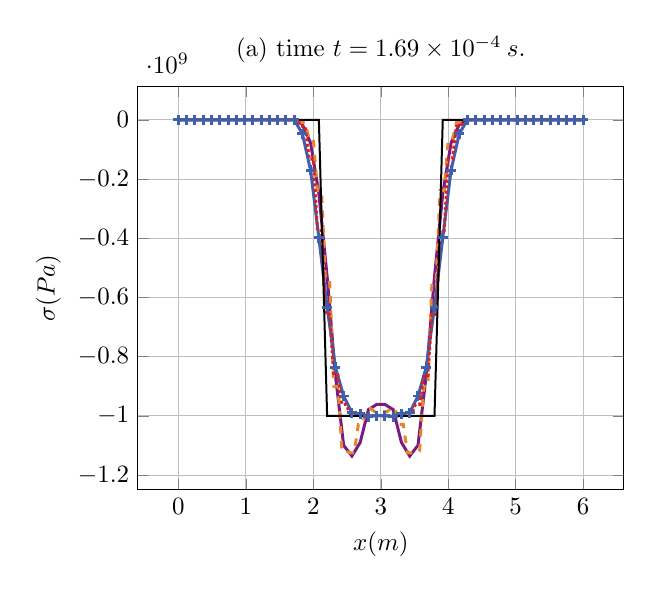
\begin{tikzpicture}[scale=0.9]
\begin{axis}[xlabel=$x (m)$,ylabel=$\sigma (Pa)$,ymajorgrids=true,xmajorgrids=true,title={(a) time $t=1.69\times 10^{-4}\: s.$}]
\addplot[Purple,very thick,mark=none,solid] coordinates {(0.0,-9.62200780097e-08) (0.122448979592,-1.92440156019e-07) (0.244897959184,-9.62200780097e-08) (0.367346938776,0.0) (0.489795918367,9.62200780097e-08) (0.612244897959,-9.62200780097e-08) (0.734693877551,-1.92440156019e-07) (0.857142857143,-9.62200780097e-08) (0.979591836735,-9.62200780097e-08) (1.10204081633,0.0) (1.22448979592,9.62200780097e-08) (1.34693877551,-9.62200780097e-08) (1.4693877551,0.0) (1.59183673469,0.0) (1.71428571429,0.0) (1.83673469388,-15437652.4848) (1.95918367347,-78183137.9185) (2.08163265306,-249067223.585) (2.20408163265,-529536815.675) (2.32653061224,-862202048.46) (2.44897959184,-1099498863.41) (2.57142857143,-1135789315.44) (2.69387755102,-1090007223.73) (2.81632653061,-978780358.738) (2.9387755102,-961497360.562) (3.0612244898,-961497360.562) (3.18367346939,-978780358.738) (3.30612244898,-1090007223.73) (3.42857142857,-1135789315.44) (3.55102040816,-1099498863.41) (3.67346938776,-862202048.46) (3.79591836735,-529536815.675) (3.91836734694,-249067223.585) (4.04081632653,-78183137.9185) (4.16326530612,-15437652.4848) (4.28571428571,-3.85185988877e-23) (4.40816326531,-9.62200780097e-08) (4.5306122449,9.62200780097e-08) (4.65306122449,9.62200780097e-08) (4.77551020408,9.62200780097e-08) (4.89795918367,-2.88660234029e-07) (5.02040816327,-9.62200780097e-08) (5.14285714286,9.62200780097e-08) (5.26530612245,1.92440156019e-07) (5.38775510204,2.88660234029e-07) (5.51020408163,9.62200780097e-08) (5.63265306122,0.0) (5.75510204082,0.0) (5.87755102041,0.0) (6.0,-9.62200780097e-08) };
\addplot[Orange,very thick,mark=none,dashed] coordinates {(0.0,0.0) (0.0606060606061,0.0) (0.121212121212,9.52481580298e-08) (0.181818181818,9.52481580298e-08) (0.242424242424,9.52481580298e-08) (0.30303030303,9.52481580298e-08) (0.363636363636,0.0) (0.424242424242,0.0) (0.484848484848,-9.52481580298e-08) (0.545454545455,-9.52481580298e-08) (0.606060606061,-1.9049631606e-07) (0.666666666667,-1.9049631606e-07) (0.727272727273,0.0) (0.787878787879,0.0) (0.848484848485,0.0) (0.909090909091,0.0) (0.969696969697,-3.85185988877e-23) (1.0303030303,-3.85185988877e-23) (1.09090909091,-9.52481580298e-08) (1.15151515152,-9.52481580298e-08) (1.21212121212,9.52481580298e-08) (1.27272727273,9.52481580298e-08) (1.33333333333,9.52481580298e-08) (1.39393939394,9.52481580298e-08) (1.45454545455,-1.9049631606e-07) (1.51515151515,-1.9049631606e-07) (1.57575757576,1.9049631606e-07) (1.63636363636,1.9049631606e-07) (1.69696969697,0.0) (1.75757575758,0.0) (1.81818181818,-9533923.2537) (1.87878787879,-9533923.2537) (1.93939393939,-67166647.336) (2.0,-67166647.336) (2.06060606061,-239339979.822) (2.12121212121,-239339979.822) (2.18181818182,-549695480.518) (2.24242424242,-549695480.518) (2.30303030303,-900240202.504) (2.36363636364,-900240202.504) (2.42424242424,-1118552245.0) (2.48484848485,-1118552245.0) (2.54545454545,-1125362633.2) (2.60606060606,-1125362633.2) (2.66666666667,-1028724363.35) (2.72727272727,-1028724363.35) (2.78787878788,-975375246.836) (2.84848484848,-975375246.836) (2.90909090909,-986009278.185) (2.9696969697,-986009278.185) (3.0303030303,-986009278.185) (3.09090909091,-986009278.185) (3.15151515152,-975375246.836) (3.21212121212,-975375246.836) (3.27272727273,-1028724363.35) (3.33333333333,-1028724363.35) (3.39393939394,-1125362633.2) (3.45454545455,-1125362633.2) (3.51515151515,-1118552245.0) (3.57575757576,-1118552245.0) (3.63636363636,-900240202.504) (3.69696969697,-900240202.504) (3.75757575758,-549695480.518) (3.81818181818,-549695480.518) (3.87878787879,-239339979.822) (3.93939393939,-239339979.822) (4.0,-67166647.336) (4.06060606061,-67166647.336) (4.12121212121,-9533923.2537) (4.18181818182,-9533923.2537) (4.24242424242,9.52481580298e-08) (4.30303030303,9.52481580298e-08) (4.36363636364,-9.52481580298e-08) (4.42424242424,-9.52481580298e-08) (4.48484848485,0.0) (4.54545454545,0.0) (4.60606060606,0.0) (4.66666666667,0.0) (4.72727272727,0.0) (4.78787878788,0.0) (4.84848484848,0.0) (4.90909090909,0.0) (4.9696969697,0.0) (5.0303030303,0.0) (5.09090909091,0.0) (5.15151515152,0.0) (5.21212121212,0.0) (5.27272727273,0.0) (5.33333333333,0.0) (5.39393939394,0.0) (5.45454545455,0.0) (5.51515151515,0.0) (5.57575757576,0.0) (5.63636363636,0.0) (5.69696969697,0.0) (5.75757575758,0.0) (5.81818181818,0.0) (5.87878787879,0.0) (5.93939393939,9.52481580298e-08) (6.0,9.52481580298e-08) };
\addplot[Blue,very thick,mark=+,solid] coordinates {(0.0,9.62200780097e-08) (0.122448979592,1.92440156019e-07) (0.244897959184,-2.88660234029e-07) (0.367346938776,-1.92440156019e-07) (0.489795918367,-9.62200780097e-08) (0.612244897959,-1.92440156019e-07) (0.734693877551,-3.84880312039e-07) (0.857142857143,-1.92440156019e-07) (0.979591836735,-9.62200780097e-08) (1.10204081633,0.0) (1.22448979592,9.62200780097e-08) (1.34693877551,-9.62200780097e-08) (1.4693877551,0.0) (1.59183673469,0.0) (1.71428571429,0.0) (1.83673469388,-46578287.5426) (1.95918367347,-171036560.611) (2.08163265306,-398499931.778) (2.20408163265,-632823078.817) (2.32653061224,-835128021.529) (2.44897959184,-932849760.398) (2.57142857143,-988852888.782) (2.69387755102,-992828858.011) (2.81632653061,-1002356300.0) (2.9387755102,-999046312.534) (3.0612244898,-999046312.534) (3.18367346939,-1002356300.0) (3.30612244898,-992828858.011) (3.42857142857,-988852888.782) (3.55102040816,-932849760.398) (3.67346938776,-835128021.529) (3.79591836735,-632823078.817) (3.91836734694,-398499931.778) (4.04081632653,-171036560.611) (4.16326530612,-46578287.5426) (4.28571428571,0.0) (4.40816326531,-9.62200780097e-08) (4.5306122449,-1.92592994439e-23) (4.65306122449,1.92440156019e-07) (4.77551020408,0.0) (4.89795918367,-9.62200780097e-08) (5.02040816327,0.0) (5.14285714286,0.0) (5.26530612245,3.85185988877e-23) (5.38775510204,1.92440156019e-07) (5.51020408163,9.62200780097e-08) (5.63265306122,0.0) (5.75510204082,9.62200780097e-08) (5.87755102041,0.0) (6.0,-9.62200780097e-08) };
\addplot[Red,very thick,mark=none,densely dotted] coordinates {(0.0,-1.9049631606e-07) (0.0606060606061,-1.9049631606e-07) (0.121212121212,0.0) (0.181818181818,0.0) (0.242424242424,9.52481580298e-08) (0.30303030303,9.52481580298e-08) (0.363636363636,-9.52481580298e-08) (0.424242424242,-9.52481580298e-08) (0.484848484848,-1.9049631606e-07) (0.545454545455,-1.9049631606e-07) (0.606060606061,0.0) (0.666666666667,0.0) (0.727272727273,0.0) (0.787878787879,0.0) (0.848484848485,0.0) (0.909090909091,0.0) (0.969696969697,-9.52481580298e-08) (1.0303030303,-9.52481580298e-08) (1.09090909091,-1.9049631606e-07) (1.15151515152,-1.9049631606e-07) (1.21212121212,-9.52481580298e-08) (1.27272727273,-9.52481580298e-08) (1.33333333333,0.0) (1.39393939394,0.0) (1.45454545455,9.52481580298e-08) (1.51515151515,9.52481580298e-08) (1.57575757576,-9.52481580298e-08) (1.63636363636,-9.52481580298e-08) (1.69696969697,0.0) (1.75757575758,0.0) (1.81818181818,-21051436.477) (1.87878787879,-21051436.477) (1.93939393939,-132631129.917) (2.0,-132631129.917) (2.06060606061,-373920143.932) (2.12121212121,-373920143.932) (2.18181818182,-657449507.004) (2.24242424242,-657449507.004) (2.30303030303,-862932918.65) (2.36363636364,-862932918.65) (2.42424242424,-960874193.44) (2.48484848485,-960874193.44) (2.54545454545,-992227161.455) (2.60606060606,-992227161.455) (2.66666666667,-998999192.727) (2.72727272727,-998999192.727) (2.78787878788,-999914743.293) (2.84848484848,-999914743.293) (2.90909090909,-999999573.105) (2.9696969697,-999999573.105) (3.0303030303,-999999573.105) (3.09090909091,-999999573.105) (3.15151515152,-999914743.293) (3.21212121212,-999914743.293) (3.27272727273,-998999192.727) (3.33333333333,-998999192.727) (3.39393939394,-992227161.455) (3.45454545455,-992227161.455) (3.51515151515,-960874193.44) (3.57575757576,-960874193.44) (3.63636363636,-862932918.65) (3.69696969697,-862932918.65) (3.75757575758,-657449507.004) (3.81818181818,-657449507.004) (3.87878787879,-373920143.932) (3.93939393939,-373920143.932) (4.0,-132631129.917) (4.06060606061,-132631129.917) (4.12121212121,-21051436.477) (4.18181818182,-21051436.477) (4.24242424242,-9.52481580298e-08) (4.30303030303,-9.52481580298e-08) (4.36363636364,9.52481580298e-08) (4.42424242424,9.52481580298e-08) (4.48484848485,0.0) (4.54545454545,0.0) (4.60606060606,0.0) (4.66666666667,0.0) (4.72727272727,0.0) (4.78787878788,0.0) (4.84848484848,0.0) (4.90909090909,0.0) (4.9696969697,0.0) (5.0303030303,0.0) (5.09090909091,0.0) (5.15151515152,0.0) (5.21212121212,0.0) (5.27272727273,0.0) (5.33333333333,0.0) (5.39393939394,0.0) (5.45454545455,0.0) (5.51515151515,0.0) (5.57575757576,0.0) (5.63636363636,0.0) (5.69696969697,0.0) (5.75757575758,0.0) (5.81818181818,0.0) (5.87878787879,0.0) (5.93939393939,-1.9049631606e-07) (6.0,-1.9049631606e-07) };
\addplot[black,thick] coordinates {(0.0,-0.0) (0.122448979592,-0.0) (0.244897959184,-0.0) (0.367346938776,-0.0) (0.489795918367,-0.0) (0.612244897959,-0.0) (0.734693877551,-0.0) (0.857142857143,-0.0) (0.979591836735,-0.0) (1.10204081633,-0.0) (1.22448979592,-0.0) (1.34693877551,-0.0) (1.4693877551,-0.0) (1.59183673469,-0.0) (1.71428571429,-0.0) (1.83673469388,-0.0) (1.95918367347,-0.0) (2.08163265306,-0.0) (2.20408163265,-1000000000.0) (2.32653061224,-1000000000.0) (2.44897959184,-1000000000.0) (2.57142857143,-1000000000.0) (2.69387755102,-1000000000.0) (2.81632653061,-1000000000.0) (2.9387755102,-1000000000.0) (3.0612244898,-1000000000.0) (3.18367346939,-1000000000.0) (3.30612244898,-1000000000.0) (3.42857142857,-1000000000.0) (3.55102040816,-1000000000.0) (3.67346938776,-1000000000.0) (3.79591836735,-1000000000.0) (3.91836734694,-0.0) (4.04081632653,-0.0) (4.16326530612,-0.0) (4.28571428571,-0.0) (4.40816326531,-0.0) (4.5306122449,-0.0) (4.65306122449,-0.0) (4.77551020408,-0.0) (4.89795918367,-0.0) (5.02040816327,-0.0) (5.14285714286,-0.0) (5.26530612245,-0.0) (5.38775510204,-0.0) (5.51020408163,-0.0) (5.63265306122,-0.0) (5.75510204082,-0.0) (5.87755102041,-0.0) (6.0,-0.0) };
%\legend{mpm 1ppc,mpm 2ppc,modmpm 1ppc,modmpm 2ppc}
\end{axis}
\end{tikzpicture}
 \phantomsubcaption \label{subfig:mpm_diffusion_10}}
  {\definecolor{Purple}{RGB}{120,28,129}
\definecolor{Orange}{RGB}{231,133,50}
\definecolor{Blue}{RGB}{63,96,174}
\definecolor{Red}{RGB}{217,33,32}
\definecolor{Duck}{RGB}{83,158,182}
\definecolor{Green}{RGB}{109,179,136}
\definecolor{Yellow}{RGB}{202,184,67}
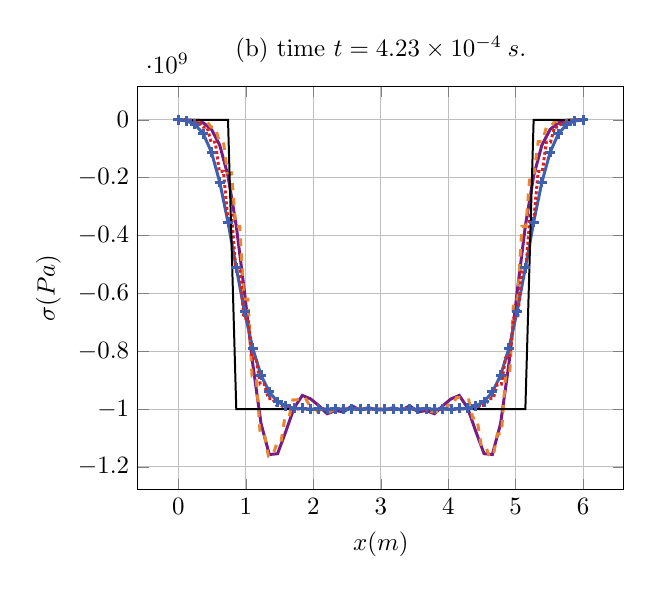
\begin{tikzpicture}[scale=0.9]
\begin{axis}[xlabel=$x (m)$,ylabel=$\sigma (Pa)$,ymajorgrids=true,xmajorgrids=true,title={(b) time $t=4.23\times 10^{-4}\: s.$}]
\addplot[Purple,very thick,mark=none,solid] coordinates {(0.0,-39934.2174897) (0.122448979592,-406302.064953) (0.244897959184,-2420460.88495) (0.367346938776,-10136844.8366) (0.489795918367,-33063216.5915) (0.612244897959,-87547121.3685) (0.734693877551,-194171704.565) (0.857142857143,-366493404.576) (0.979591836735,-596875114.898) (1.10204081633,-845116689.368) (1.22448979592,-1050481005.19) (1.34693877551,-1157297307.0) (1.4693877551,-1154376682.02) (1.59183673469,-1077374033.62) (1.71428571429,-995689036.388) (1.83673469388,-952936697.469) (1.95918367347,-964832377.273) (2.08163265306,-988568067.368) (2.20408163265,-1016260759.09) (2.32653061224,-1005179173.62) (2.44897959184,-1009892551.13) (2.57142857143,-988773783.034) (2.69387755102,-1003829596.99) (2.81632653061,-995025027.704) (2.9387755102,-1003213108.71) (3.0612244898,-1003213108.71) (3.18367346939,-995025027.704) (3.30612244898,-1003829596.99) (3.42857142857,-988773783.034) (3.55102040816,-1009892551.13) (3.67346938776,-1005179173.62) (3.79591836735,-1016260759.09) (3.91836734694,-988568067.368) (4.04081632653,-964832377.273) (4.16326530612,-952936697.469) (4.28571428571,-995689036.388) (4.40816326531,-1077374033.62) (4.5306122449,-1154376682.02) (4.65306122449,-1157297307.0) (4.77551020408,-1050481005.19) (4.89795918367,-845116689.368) (5.02040816327,-596875114.898) (5.14285714286,-366493404.576) (5.26530612245,-194171704.565) (5.38775510204,-87547121.3685) (5.51020408163,-33063216.5915) (5.63265306122,-10136844.8366) (5.75510204082,-2420460.88495) (5.87755102041,-406302.064953) (6.0,-39934.2174897) };
\addplot[Orange,very thick,mark=none,dashed] coordinates {(0.0,-10429.0753611) (0.0606060606061,-10429.0753611) (0.121212121212,-161982.808053) (0.181818181818,-161982.808053) (0.242424242424,-1267409.75703) (0.30303030303,-1267409.75703) (0.363636363636,-6575307.60772) (0.424242424242,-6575307.60772) (0.484848484848,-25213047.7874) (0.545454545455,-25213047.7874) (0.606060606061,-75630068.1866) (0.666666666667,-75630068.1866) (0.727272727273,-183565723.323) (0.787878787879,-183565723.323) (0.848484848485,-368376215.18) (0.909090909091,-368376215.18) (0.969696969697,-620238104.743) (1.0303030303,-620238104.743) (1.09090909091,-886041263.042) (1.15151515152,-886041263.042) (1.21212121212,-1086232263.3) (1.27272727273,-1086232263.3) (1.33333333333,-1162610811.08) (1.39393939394,-1162610811.08) (1.45454545455,-1121800356.23) (1.51515151515,-1121800356.23) (1.57575757576,-1031608883.18) (1.63636363636,-1031608883.18) (1.69696969697,-967968470.151) (1.75757575758,-967968470.151) (1.81818181818,-960540680.349) (1.87878787879,-960540680.349) (1.93939393939,-986227377.719) (2.0,-986227377.719) (2.06060606061,-1007602191.25) (2.12121212121,-1007602191.25) (2.18181818182,-1009726046.8) (2.24242424242,-1009726046.8) (2.30303030303,-1002072997.71) (2.36363636364,-1002072997.71) (2.42424242424,-997465464.463) (2.48484848485,-997465464.463) (2.54545454545,-998318352.653) (2.60606060606,-998318352.653) (2.66666666667,-1000280134.99) (2.72727272727,-1000280134.99) (2.78787878788,-1000550813.71) (2.84848484848,-1000550813.71) (2.90909090909,-999915604.91) (2.9696969697,-999915604.91) (3.0303030303,-999915604.91) (3.09090909091,-999915604.91) (3.15151515152,-1000550813.71) (3.21212121212,-1000550813.71) (3.27272727273,-1000280134.99) (3.33333333333,-1000280134.99) (3.39393939394,-998318352.653) (3.45454545455,-998318352.653) (3.51515151515,-997465464.463) (3.57575757576,-997465464.463) (3.63636363636,-1002072997.71) (3.69696969697,-1002072997.71) (3.75757575758,-1009726046.8) (3.81818181818,-1009726046.8) (3.87878787879,-1007602191.25) (3.93939393939,-1007602191.25) (4.0,-986227377.719) (4.06060606061,-986227377.719) (4.12121212121,-960540680.349) (4.18181818182,-960540680.349) (4.24242424242,-967968470.151) (4.30303030303,-967968470.151) (4.36363636364,-1031608883.18) (4.42424242424,-1031608883.18) (4.48484848485,-1121800356.23) (4.54545454545,-1121800356.23) (4.60606060606,-1162610811.08) (4.66666666667,-1162610811.08) (4.72727272727,-1086232263.3) (4.78787878788,-1086232263.3) (4.84848484848,-886041263.042) (4.90909090909,-886041263.042) (4.9696969697,-620238104.743) (5.0303030303,-620238104.743) (5.09090909091,-368376215.18) (5.15151515152,-368376215.18) (5.21212121212,-183565723.323) (5.27272727273,-183565723.323) (5.33333333333,-75630068.1866) (5.39393939394,-75630068.1866) (5.45454545455,-25213047.7874) (5.51515151515,-25213047.7874) (5.57575757576,-6575307.60772) (5.63636363636,-6575307.60772) (5.69696969697,-1267409.75703) (5.75757575758,-1267409.75703) (5.81818181818,-161982.808054) (5.87878787879,-161982.808054) (5.93939393939,-10429.0753609) (6.0,-10429.0753609) };
\addplot[Blue,very thick,mark=+,solid] coordinates {(0.0,-508931.478279) (0.122448979592,-3748025.68591) (0.244897959184,-16014385.4746) (0.367346938776,-47881742.3505) (0.489795918367,-112174746.169) (0.612244897959,-215592738.441) (0.734693877551,-354671855.848) (0.857142857143,-511212799.02) (0.979591836735,-663838312.129) (1.10204081633,-790213464.162) (1.22448979592,-883647482.448) (1.34693877551,-941000619.105) (1.4693877551,-974959939.111) (1.59183673469,-988927861.484) (1.71428571429,-997557909.852) (1.83673469388,-997805889.972) (1.95918367347,-1000931915.66) (2.08163265306,-998709339.041) (2.20408163265,-1001197182.01) (2.32653061224,-998859728.815) (2.44897959184,-1001017871.89) (2.57142857143,-999150004.014) (2.69387755102,-1000640138.33) (2.81632653061,-999602146.851) (2.9387755102,-1000134970.66) (3.0612244898,-1000134970.66) (3.18367346939,-999602146.851) (3.30612244898,-1000640138.33) (3.42857142857,-999150004.014) (3.55102040816,-1001017871.89) (3.67346938776,-998859728.815) (3.79591836735,-1001197182.01) (3.91836734694,-998709339.041) (4.04081632653,-1000931915.66) (4.16326530612,-997805889.972) (4.28571428571,-997557909.852) (4.40816326531,-988927861.484) (4.5306122449,-974959939.111) (4.65306122449,-941000619.105) (4.77551020408,-883647482.448) (4.89795918367,-790213464.162) (5.02040816327,-663838312.129) (5.14285714286,-511212799.02) (5.26530612245,-354671855.848) (5.38775510204,-215592738.441) (5.51020408163,-112174746.169) (5.63265306122,-47881742.3505) (5.75510204082,-16014385.4746) (5.87755102041,-3748025.68591) (6.0,-508931.478279) };
\addplot[Red,very thick,mark=none,densely dotted] coordinates {(0.0,-61223.9335744) (0.0606060606061,-61223.9335744) (0.121212121212,-884894.710625) (0.181818181818,-884894.710625) (0.242424242424,-6003361.51961) (0.30303030303,-6003361.51961) (0.363636363636,-25575128.3809) (0.424242424242,-25575128.3809) (0.484848484848,-77365275.2782) (0.545454545455,-77365275.2782) (0.606060606061,-178548645.631) (0.666666666667,-178548645.631) (0.727272727273,-330659471.659) (0.787878787879,-330659471.659) (0.848484848485,-511731335.491) (0.909090909091,-511731335.491) (0.969696969697,-686005012.829) (1.0303030303,-686005012.829) (1.09090909091,-823733433.992) (1.15151515152,-823733433.992) (1.21212121212,-914145742.521) (1.27272727273,-914145742.521) (1.33333333333,-963861687.734) (1.39393939394,-963861687.734) (1.45454545455,-986895334.229) (1.51515151515,-986895334.229) (1.57575757576,-995919063.725) (1.63636363636,-995919063.725) (1.69696969697,-998912836.991) (1.75757575758,-998912836.991) (1.81818181818,-999753499.27) (1.87878787879,-999753499.27) (1.93939393939,-999952757.55) (2.0,-999952757.55) (2.06060606061,-999992418.488) (2.12121212121,-999992418.488) (2.18181818182,-999998994.239) (2.24242424242,-999998994.239) (2.30303030303,-999999891.711) (2.36363636364,-999999891.711) (2.42424242424,-999999990.727) (2.48484848485,-999999990.727) (2.54545454545,-999999999.438) (2.60606060606,-999999999.438) (2.66666666667,-999999999.942) (2.72727272727,-999999999.942) (2.78787878788,-1000000000.02) (2.84848484848,-1000000000.02) (2.90909090909,-999999999.993) (2.9696969697,-999999999.993) (3.0303030303,-999999999.993) (3.09090909091,-999999999.993) (3.15151515152,-1000000000.02) (3.21212121212,-1000000000.02) (3.27272727273,-999999999.942) (3.33333333333,-999999999.942) (3.39393939394,-999999999.438) (3.45454545455,-999999999.438) (3.51515151515,-999999990.727) (3.57575757576,-999999990.727) (3.63636363636,-999999891.711) (3.69696969697,-999999891.711) (3.75757575758,-999998994.239) (3.81818181818,-999998994.239) (3.87878787879,-999992418.488) (3.93939393939,-999992418.488) (4.0,-999952757.55) (4.06060606061,-999952757.55) (4.12121212121,-999753499.27) (4.18181818182,-999753499.27) (4.24242424242,-998912836.991) (4.30303030303,-998912836.991) (4.36363636364,-995919063.725) (4.42424242424,-995919063.725) (4.48484848485,-986895334.229) (4.54545454545,-986895334.229) (4.60606060606,-963861687.734) (4.66666666667,-963861687.734) (4.72727272727,-914145742.521) (4.78787878788,-914145742.521) (4.84848484848,-823733433.992) (4.90909090909,-823733433.992) (4.9696969697,-686005012.829) (5.0303030303,-686005012.829) (5.09090909091,-511731335.491) (5.15151515152,-511731335.491) (5.21212121212,-330659471.659) (5.27272727273,-330659471.659) (5.33333333333,-178548645.631) (5.39393939394,-178548645.631) (5.45454545455,-77365275.2782) (5.51515151515,-77365275.2782) (5.57575757576,-25575128.3809) (5.63636363636,-25575128.3809) (5.69696969697,-6003361.51961) (5.75757575758,-6003361.51961) (5.81818181818,-884894.710625) (5.87878787879,-884894.710625) (5.93939393939,-61223.9335744) (6.0,-61223.9335744) };
\addplot[black,thick] coordinates {(0.0,-0.0) (0.122448979592,-0.0) (0.244897959184,-0.0) (0.367346938776,-0.0) (0.489795918367,-0.0) (0.612244897959,-0.0) (0.734693877551,-0.0) (0.857142857143,-1000000000.0) (0.979591836735,-1000000000.0) (1.10204081633,-1000000000.0) (1.22448979592,-1000000000.0) (1.34693877551,-1000000000.0) (1.4693877551,-1000000000.0) (1.59183673469,-1000000000.0) (1.71428571429,-1000000000.0) (1.83673469388,-1000000000.0) (1.95918367347,-1000000000.0) (2.08163265306,-1000000000.0) (2.20408163265,-1000000000.0) (2.32653061224,-1000000000.0) (2.44897959184,-1000000000.0) (2.57142857143,-1000000000.0) (2.69387755102,-1000000000.0) (2.81632653061,-1000000000.0) (2.9387755102,-1000000000.0) (3.0612244898,-1000000000.0) (3.18367346939,-1000000000.0) (3.30612244898,-1000000000.0) (3.42857142857,-1000000000.0) (3.55102040816,-1000000000.0) (3.67346938776,-1000000000.0) (3.79591836735,-1000000000.0) (3.91836734694,-1000000000.0) (4.04081632653,-1000000000.0) (4.16326530612,-1000000000.0) (4.28571428571,-1000000000.0) (4.40816326531,-1000000000.0) (4.5306122449,-1000000000.0) (4.65306122449,-1000000000.0) (4.77551020408,-1000000000.0) (4.89795918367,-1000000000.0) (5.02040816327,-1000000000.0) (5.14285714286,-1000000000.0) (5.26530612245,-0.0) (5.38775510204,-0.0) (5.51020408163,-0.0) (5.63265306122,-0.0) (5.75510204082,-0.0) (5.87755102041,-0.0) (6.0,-0.0) };
%\legend{mpm 1ppc,mpm 2ppc,modmpm 1ppc,modmpm 2ppc}
\end{axis}
\end{tikzpicture}
 \phantomsubcaption \label{subfig:mpm_diffusion_25}}\\
  {\definecolor{Purple}{RGB}{120,28,129}
\definecolor{Orange}{RGB}{231,133,50}
\definecolor{Blue}{RGB}{63,96,174}
\definecolor{Red}{RGB}{217,33,32}
\definecolor{Duck}{RGB}{83,158,182}
\definecolor{Green}{RGB}{109,179,136}
\definecolor{Yellow}{RGB}{202,184,67}
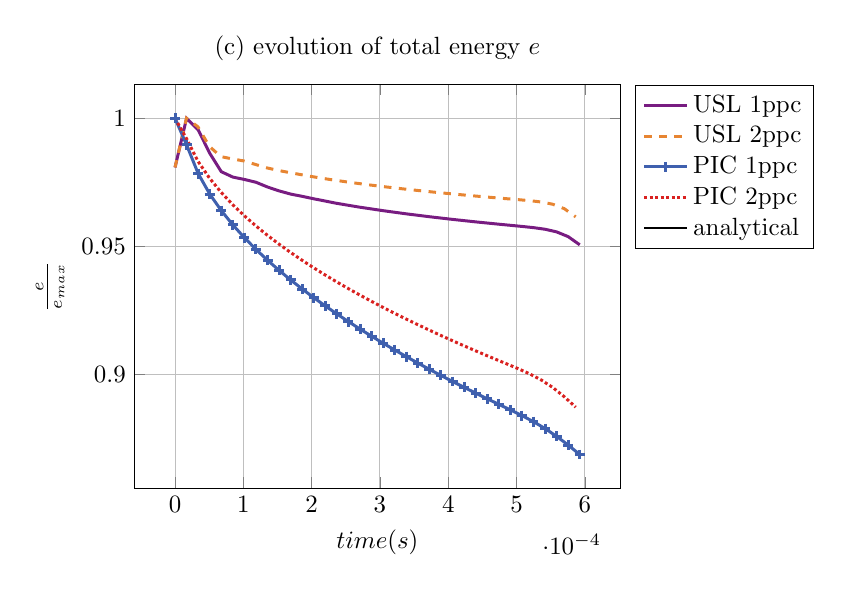
\begin{tikzpicture}[scale=0.9]
\begin{axis}[xlabel=$time (s)$,ylabel=$\frac{e}{e_{max}}$,ymajorgrids=true,xmajorgrids=true,title={(c) evolution of total energy $e$}, legend pos=outer north east]
\addplot[Purple,very thick,mark=none,solid] coordinates {(0.0,0.980776775206) (1.69272151355e-05,1.0) (3.38544302711e-05,0.995486386818) (5.07816454066e-05,0.986335480918) (6.77088605422e-05,0.979118179787) (8.46360756777e-05,0.977011836735) (0.000101563290813,0.976083552705) (0.000118490505949,0.974985958077) (0.000135417721084,0.973132007483) (0.00015234493622,0.971614043952) (0.000169272151355,0.970370597838) (0.000186199366491,0.969484052645) (0.000203126581626,0.968527091175) (0.000220053796762,0.967645365047) (0.000236981011898,0.966743210911) (0.000253908227033,0.965982183586) (0.000270835442169,0.965231974397) (0.000287762657304,0.964563191524) (0.00030468987244,0.96388114719) (0.000321617087575,0.963263530823) (0.000338544302711,0.962646353557) (0.000355471517846,0.962084695394) (0.000372398732982,0.961521764293) (0.000389325948117,0.961001071279) (0.000406253163253,0.960479919884) (0.000423180378389,0.959994795728) (0.000440107593524,0.959510651477) (0.00045703480866,0.959056403386) (0.000473962023795,0.958603029859) (0.000490889238931,0.958172736022) (0.000507816454066,0.957731808745) (0.000524743669202,0.957261239502) (0.000541670884337,0.956629022745) (0.000558598099473,0.95560284594) (0.000575525314608,0.953743784185) (0.000592452529744,0.950544066664) };
\addplot[Orange,very thick,mark=none,dashed] coordinates {(0.0,0.980776775206) (1.67562331645e-05,1.0) (3.3512466329e-05,0.996663809337) (5.02686994934e-05,0.98900666995) (6.70249326579e-05,0.985020324447) (8.37811658224e-05,0.984110580813) (0.000100537398987,0.983326915208) (0.000117293632151,0.981979184866) (0.000134049865316,0.980638155666) (0.00015080609848,0.979617302856) (0.000167562331645,0.978778886884) (0.000184318564809,0.977968446843) (0.000201074797974,0.977176694993) (0.000217831031138,0.976440965591) (0.000234587264303,0.975764557777) (0.000251343497467,0.975128766754) (0.000268099730632,0.974522184343) (0.000284855963796,0.973943735564) (0.000301612196961,0.973393220953) (0.000318368430125,0.972867749193) (0.00033512466329,0.972363947434) (0.000351880896454,0.971879647077) (0.000368637129618,0.971413467384) (0.000385393362783,0.970964070517) (0.000402149595947,0.97053007437) (0.000418905829112,0.970110254428) (0.000435662062276,0.969703595912) (0.000452418295441,0.969309210173) (0.000469174528605,0.96892621672) (0.00048593076177,0.968553101725) (0.000502686994934,0.968183689821) (0.000519443228099,0.96779053395) (0.000536199461263,0.967278784767) (0.000552955694428,0.96640240077) (0.000569711927592,0.964686590438) (0.000586468160757,0.961481917033) };
\addplot[Blue,very thick,mark=+,solid] coordinates {(0.0,1.0) (1.69272151355e-05,0.9896) (3.38544302711e-05,0.97840192) (5.07816454066e-05,0.970395814144) (6.77088605422e-05,0.963922377931) (8.46360756777e-05,0.958330092512) (0.000101563290813,0.953327939993) (0.000118490505949,0.948758714644) (0.000135417721084,0.944525461648) (0.00015234493622,0.940563061208) (0.000169272151355,0.936825160363) (0.000186199366491,0.933277336034) (0.000203126581626,0.929893178182) (0.000220053796762,0.926651891851) (0.000236981011898,0.923536752237) (0.000253908227033,0.92053406787) (0.000270835442169,0.917632461061) (0.000287762657304,0.914822354268) (0.00030468987244,0.912095594541) (0.000321617087575,0.909445173164) (0.000338544302711,0.906865012545) (0.000355471517846,0.904349801607) (0.000372398732982,0.901894866831) (0.000389325948117,0.899496069935) (0.000406253163253,0.897149725755) (0.000423180378389,0.894852535658) (0.000440107593524,0.892601494491) (0.00045703480866,0.890393110082) (0.000473962023795,0.888218874172) (0.000490889238931,0.886052220178) (0.000507816454066,0.883829497068) (0.000524743669202,0.881442958718) (0.000541670884337,0.878767030396) (0.000558598099473,0.875715616111) (0.000575525314608,0.872297097702) (0.000592452529744,0.868628627691) };
\addplot[Red,very thick,mark=none,densely dotted] coordinates {(0.0,1.0) (1.67562331645e-05,0.9921) (3.3512466329e-05,0.98321470125) (5.02686994934e-05,0.976674798128) (6.70249326579e-05,0.971199634535) (8.37811658224e-05,0.966410687731) (0.000100537398987,0.962109118378) (0.000117293632151,0.958172229577) (0.000134049865316,0.954520707917) (0.00015080609848,0.951100328411) (0.000167562331645,0.947872098186) (0.000184318564809,0.944806876372) (0.000201074797974,0.941882214857) (0.000217831031138,0.939080387869) (0.000234587264303,0.936387108509) (0.000251343497467,0.933790661554) (0.000268099730632,0.931281298637) (0.000284855963796,0.928850804847) (0.000301612196961,0.926492180888) (0.000318368430125,0.924199405234) (0.00033512466329,0.92196725296) (0.000351880896454,0.919791155586) (0.000368637129618,0.917667091102) (0.000385393362783,0.915591496621) (0.000402149595947,0.913561198187) (0.000418905829112,0.911573353815) (0.000435662062276,0.909625405615) (0.000452418295441,0.907714970883) (0.000469174528605,0.905838699657) (0.00048593076177,0.903984815557) (0.000502686994934,0.902108349787) (0.000519443228099,0.900090874846) (0.000536199461263,0.89772781162) (0.000552955694428,0.894800303924) (0.000569711927592,0.891215939989) (0.000586468160757,0.8871100207) };
\addplot[black,thick] coordinates {(0.,1.) (0.0000001,1.)};
\legend{USL 1ppc,USL 2ppc,PIC 1ppc,PIC 2ppc,analytical}
\end{axis}
\end{tikzpicture}

%%% Local Variables: 
%%% mode: latex
%%% TeX-master: "../../mainManuscript"
%%% End:
 \phantomsubcaption \label{subfig:mpm_energies}}
  \caption{Comparison USL solutions using either velocity update or interpolation and exact solution of the bars impact problem for various discretizations. (a)--(b) comparison of stress profiles at several time steps (c) evolution of total energy. Parameters: $CFL=0.7$ ; $v_0=\frac{1}{200}\sqrt{\frac{E}{\rho}}$.}
  \label{fig:mpm_diffusion}
\end{figure}

\subsection{Strategy for reducing oscillations and diffusion}
In this, we are concerned here with the accurate solution of hyperbolic problems in solid undergoing finite deformations. Although the MPM enables an efficient management of large strains, the oscillations it suffers from do not allow to accurately capture waves propagating in a medium. The above numerical results however suggest that the numerical noise can be removed by using an interpolation instead of an update of material points velocity, at the cost of additional diffusion. The point of view adopted in this thesis is that the numerical diffusion is essentially due to the projection of fields from particles to nodes and back tha spread the information. Hence, a reduction of the domain of influence of material points is preferred to a widening, as GIMP, BSMPM and DDMPM propose. 
As a consequence, a combination of the  \textit{Discontinuous Galerkin} approximation (DG) and the transfer of velocity from nodes to particles originally developed for PIC is proposed within the MPM. These two features are expected to respectively enable numerical diffusion and spurious osccilations. It is worth noticing that attention is paid to impact problems which solutions are mostly unregular so that high-order approximations, as investigated in \cite{MPM_BSpline2} or \cite{BsplineMPM}, are not considered here. 
 
% Dire un mot sur le HighOrder MPM qui n'est pas forcément désiré car on cherche à approcher des discontinuités.


%%% Local Variables: 
%%% mode: latex
%%% TeX-master: "../mainManuscript"
%%% End:


\section{Extension of the MPM to discontinuous Galerkin approximation}
\label{sec:DGMPM}
%The extension of the material point method to the DG approximation has been motivated in the previous section and is carried out hereinafter.
After a brief historical review of DG methods, the Discontinuous Galerkin Material Point Method is derived within the large strain framework with a total Lagrangian formulation. It will be seen that this new numerical approach makes use of the approximate-state Riemann solver developed in section \ref{sec:riemann_solvers} to compute intercell terms which purpose is to connect elements together. At last, the DGMPM solution scheme will be provided for hyperbolic problems.

\subsection{The discontinuous Galerkin approximation}
The DG approximation was first introduced in the context of the finite element method for the solution of the neutron transport equation \cite{NeutronDG}. This hyperbolic equation describes the advection of the angular flux which quantifies the amount of neutrons at a given location. Since neutrons can lie in a cell of a finite element mesh while its neighbors are empty, the need of describing discontinuities of the primal field across elements interfaces within a FEM context arised. Hence, an approximate solution was seeked by the Galerkin method, in a domain discretized with triangular elements by means of Lagrange polynomials that can be discontinuous across the cells. This approach amounts to duplicate the nodes of the mesh so that the support of each shape function reduces to one finite element. Those early works have launched a serie of developments of the \textbf{Discontinuous Galerkin Finite Element Method} (DGFEM) for parabolic \cite{Arnold_IPM}, elliptic \cite{Hansbo_DGsolid,Noel_HEDG}, and hyperbolic problems \cite{Cockburn}. Indeed, the DGFEM gained more and more popularity since the 80's, even for problems that do not involve discontinuities, on account of its ability to locally handle high-order approximation and its highly parallelizable nature. 
Researches conducted in the context of hyperbolic problems, of particular interest here, enabled the introduction of numerical tools developed for Finite Volume Methods (FVM) within finite element schemes.
Namely, the use of suitable \textit{slope limiters} \cite{vanLeer_Limiters} based on the \textit{total variation} \cite{Harten_TVD} enables the formulation of flexible numerical methods in which a good resolution of discontinuities is possible without destroying the accuracy in smooth regions. Furthermore, these approaches can easily handle mesh-adaption strategies by dint of the relaxation of fields continuity. Nevertheless mesh tangling problems do not vanish.
Thus, the introduction of DG approximation in the MPM should lead to a numerical method that benefits from both FEM and FVM features and enables local high-order approximation while avoiding mesh entanglement instabilities.


% %%%%%%%%%%%%%%%%%%%%%%%%%%%%%%%%%%%%%%%%%%%%%%%%%%%%%%%%%%%%%
% % Hyperbolic
% The \textit{discontinuous Galerkin (DG)} approximation enables to build numerical schemes that benefit from both finite element and finite volume methods. 
% Parler des limiteurs \cite{vanLeer_Limiters} pour atteindre la notion de schéma TVB et TVDM (TVD \cite{Harten_TVD}). Extension to RK so that the scheme can reach locally high order accuracy. In addition, the same order of accuracy is reached for velocity and gradients within a finite element framework when the weak form is based on a conservation laws system. 

% % In parallel, for parabolic or elliptic
% \cite[parabolic+penalties]{Arnold_IPM},\cite{Hansbo_DGsolid},\cite[elliptic]{Noel_HEDG}: Three field Hu-Washizu variational formulation ; assumed form of deformation gradient ; Total Lagrangian ; penalization of displacement jumps; Advantages--Drawbacks in note books

% % Introduction of HDG
% \cite{Cockburn_HDG0},\cite{Cockburn_HDG1},\cite{Cockburn_HDG2}: HDG for elliptic problems (differrence between LDG-H and HDG ?)

% % Recently extended to hyperbolic problems in solid dynamics
% \cite{NGuyen_HDG} for application to solid mechanics and extension to hyperbolic problems. Solved for displacement with enforced continuity across elements interfaces. Does not use the characteristic structure as what is done in finite volumes or original DGFEM

% However, all those approaches based on the primal field do not use the characterisitc structure. Dans l'état, ça ne peut pas être appliqué à la méca des solides puisque l'on est obligé d'imposer la continuité du champ de déplacement et donc de formuler le problème en u.
% \begin{itemize}
% \item \cite{Chavent_Salzano,Chavent_Cockburn,Cockburn_Shu,DGFEM_CFL,Cockburn}:
% \item \cite{Chavent_Salzano}--\cite{Cockburn} developments of DGFEM (mainly for fluid mechanics ?)
% \item \cite[parabolic+penalties]{Arnold_IPM},\cite{Hansbo_DGsolid},\cite[elliptic]{Noel_HEDG}: Three field Hu-Washizu variational formulation ; assumed form of deformation gradient ; Total Lagrangian ; penalization of displacement jumps; Advantages--Drawbacks in note books
% \item \cite{Cockburn_HDG0},\cite{Cockburn_HDG1},\cite{Cockburn_HDG2}: HDG for elliptic problems (differrence between LDG-H and HDG ?)
% \item \cite{NGuyen_HDG} for application to solid mechanics and extension to hyperbolic problems. Solved for displacement with enforced continuity across elements interfaces. Does not use the characteristic structure as what is done in finite volumes or original DGFEM
% \item \cite{DGPIC,DGPIC_maxwell}: application to PIC
% \end{itemize}


% RKDG - limiters - TVD - CFL - HDG (steady convection-diffusion problem (elliptic problem)) - HE DG
% Applied to steady solid mechanics problems for the ability of local high order approximation ?
% Continuity of displacement enforced through Lagrange multipliers. Benefits from superconvergence properties. A priori on utilise plus du HDG en méca du solide \cite[ALE]{NGuyen_HDG} + postprocessing pour le champ de déplacement + implicit en dynamique. Originally developed in \cite{Cockburn_HDG0}: "we may define more generally as a hybrid method any finite element method based on a formulation where one unknown is a function, or some of its derivatives, on the set $\Omega$, and the other unknown is the trace of some of its derivatives of the same function, or the trace of the function itself, along the boundaries of the set K". Numerical traces \cite{Cockburn_HDG1}


\subsection{Derivation of the DGMPM}
Consider again a continuum solid body with volume $\Omega_t$ within the time interval $\tau$. The DGMPM is expected to provide a material description of a deformation so that an approximate solution of a Lagrangian system of conservation laws written in conservative form is seeked. Recall that such a conservative form for some vector of conserved quantities $\Wcb$ reads, in Cartesian coordinates system:
\begin{equation}
  \label{eq:conservative_form}
  \drond{\Wcb}{t} + \sum_{\alpha=1}^D \drond{\Fcb\cdot \vect{e}_\alpha}{X_\alpha} = \Scb \quad \forall \vect{X},t \in \Omega_0 \times \tau
\end{equation}

\subsubsection{The DGMPM discretization}
As for MPM, a continuum body $\Omega_t$ is discretized within the time interval $\tau$ into a set of $N_p$ material points in an arbitrary Cartesian grid made of  $N_n$ nodes and $E$ non-overlapping cells of volume $\Omega^e$. The boundary of the domain is again defined by the set of edges separating empty cells from those containing particles (see figure \ref{fig:domain} for a two-dimensional example).
In addition, the reference mass density is described in the computational grid by means of the delta Dirac characteristic function and particles masses:
\begin{equation}
  \label{eq:mass_density_DGMPM}
  \rho_0\(\vect{X}\) =  \sum_{p=1}^{N_p} m_p \delta\(\vect{X}^p - \vect{X}\)
\end{equation}
where $\Omega_0$ denotes the reference configuration of the continuum. In a similar manenr to FEM and MPM, the vector of conserved quantities is approximated on the mesh by:
\begin{equation}
  \label{eq:DGMPM_node2points}
  \Wcb(\vect{X},t) = \sum^{N_n}_{i=1} S_{i}(\vect{X})\Wcb^i(t) 
\end{equation}
with $\Wcb^i$ the vector of conserved quantities at node $i$, and $S_{i}(\vect{X})$ tha shape function attached to it. Note that the convention of denoting particle and nodal fields by $p$ and $(i,j)$ still holds in this section.

\subsubsection{Weak formulation of the continuum problem}
Multiplying equation \eqref{eq:conservative_form} by a test function $\Vcb$ yields the weak formulation of the problem:
\begin{equation}
  \label{eq:weak_form}
  \begin{aligned}
    &\text{Find $\Wcb \in \Vscr_h^1$ such that} \\
    &\int_{\Omega_t} \drond{\Wcb}{t} \vect{\Vc} \: d\Omega + \int_{\Omega_t}   \drond{\Fcb_\alpha}{X_\alpha}\vect{\Vc} \: d\Omega    = \int_{\Omega_t} \Scb \vect{\Vc} \: d\Omega \quad \forall \: \vect{\Vc},t \in  \Vscr_h^1\times \tau
  \end{aligned}
\end{equation}
The key idea of DG methods is to allow jump of fields across mesh elements faces by using broken polynomial spaces for the approximate solution \cite[Ch.1]{DiPietro}:
\begin{equation}
\Vscr^k = \{ \Vcb \in H^k\Omega^e) \} \quad ;\quad \Vscr_h^k = \{\Vcb \in \Pscr^k(\Omega^e) \} \subset \Vscr^k
\end{equation}
with $H^k(\Omega^e)$, the Sobolev space and $\Pscr^k(\Omega^e)$, the space of polynomials of degree $k$ in $\Omega^e$. We restrict our attention here to linear polynomials ($k=1$). Those broken polynomials spaces allows to rewrite the weak form element-wise. After integration by part, one gets:
\begin{equation}
  \label{eq:DGMPM_weak_form}
  \begin{aligned}
    &\text{Find $\Wcb \in \Vscr_h^1$ such that} \\
    &\int_{\Omega^e} \drond{\Wcb}{t} \vect{\Vc} \: d\Omega - \int_{\Omega^e} \Fcb_\alpha  \drond{\vect{\Vc}}{X_\alpha} \: d\Omega   + \int_{\partial \Omega^e} \(\Fcb\cdot \vect{N}\)  \vect{\Vc} \: d\Gamma = \int_{\Omega^e} \Scb \vect{\Vc} \: d\Omega \quad \forall \: \vect{\Vc},e,t \in  \Vscr_h^1\times \[1,E\]\times \tau
  \end{aligned}
\end{equation}
where $\partial \Omega^e$ is the boundary of the $e$th element with outward normal vector $\vect{N}$. The dot operator $\Fcb\cdot \vect{N}$ denotes the inner product between the outward normal vector and every component of the flux, thus yielding the intercell flux, written $\Fcb_N$ for simplicity. Next, the introduction of specific fields:
\begin{equation}
  \label{eq:specific_quantities}
  \Wcb = \rho_0 \bar{\Wcb} \quad ; \quad \Fcb_\alpha = \rho_0 \bar{\Fcb}_\alpha \quad ; \quad \Scb = \rho_0 \bar{\Scb}
\end{equation}
combined with the definition of mass density \eqref{eq:mass_density_DGMPM}, leads to the following total Lagrangian formulation:
%Such a discretization of the reference mass density combined with the writing of Lagrangian conservation laws \eqref{eq:conservative_form} yields a total Lagrangian formulation, and equation \eqref{eq:DGMPM_weak_form} thus reads:
\begin{equation} 
  \label{eq:DGMPM_discrete_weak}
  \sum_{p=1}^{N_p} m_p\[\drond{\bar{\Wcb}}{t}  \vect{\Vc} - \bar{\Fcb}_{\alpha} \drond{\vect{\Vc}}{X_\alpha} -\bar{\Scb}  \vect{\Vc} \]_{|\vect{X}=\vect{X}^p} + \int_{\partial \Omega^e} \Fcb_N  \vect{\Vc} \: d\Gamma = 0 \quad \forall \: \vect{\Vc},e,t \in  \Vscr_h^1\times \[1,E\]\times \tau
\end{equation}

At last, introduction of the DGMPM approximation \eqref{eq:DGMPM_node2points} and arbitrariness of the test field in the weak form \eqref{eq:DGMPM_discrete_weak} provide the semi-discrete system that must be solved on the grid:
\begin{equation}
  \label{eq:DGMPM_semi_discrete}
  \sum_{p=1}^{N_p}\[ S_{ip} m_p S_{jp} \drond{\bar{\Wcb}^j}{t}  - \drond{S_{ip}}{X_\alpha} m_p S_{jp} \bar{\Fcb}^j_{\alpha} - S_{ip} m_p \bar{\Scb}^p\] + \int_{\Gamma_e} S_i(\vect{X}) \Fcb_N  \: d\Gamma =  0  \quad \forall \: e,t \in  \times \[1,E\]\times \tau
\end{equation}
or, in matrix form:
\begin{equation}
  \label{eq:DGMPM_semi_discrete_matrix}
  M_{ij} \drond{\bar{\Wcb}_j}{t} - K^\alpha_{ij} \bar{\Fcb}^j_{\alpha} - \Scb^i + \vect{\hat{\Fc}}^i = \vect{0}  
\end{equation}
Here again, particles plays the role of integration points in volume integrals owing to the delta Dirac characteristic function. Hence, the consistent mass matrix $M_{ij}$ may also be singular due to reduced integration so that the diagonally lumped mass matrix $M^L_i$ is used.
\begin{remark}
  \label{rq:DGPIC}
  An extension of PIC to DG approximation for the solution of Maxwell's equations is proposed in \cite{DGPIC_maxwell} and \cite{Stindl_DGPIC} in which different projections of fields between the grid and particles are used. Although those methods allow local high-order approximation, particles do not carry every fields so that the DGPIC, as the original PIC, cannot be considered as a fully Lagrangian approach. In addition, the use of Gauss quadrature rule for volume integrals of the weak form makes this approach different from that developed in the following.
\end{remark}
The discrete system is derived by discretizing the time interval $\tau$ into $N_t$ subintervals and using the explicit forward Euler method:
%Finally, the explicit forward Euler time discretization of $\tau$ in $N_t$ subinterval is perfomed, leading to the discrete system:
\begin{equation}
  \label{eq:DGMPM_discrete}
  M^L_i \frac{\bar{\Wcb}^{i,n+1} - \bar{\Wcb}^{i,n}}{\Delta t^{n} } = K^\alpha_{ij} \bar{\Fcb}_{\alpha}^{j,n} + \Scb^{i,n}- \vect{\hat{\Fc}}^{i,n}  
\end{equation}
where again, the superscripts $(\bullet)^{k,l}$ denote a field evaluated at node $k$ and time step $l$. Note that in general the source term $\Scb$ may depend on the vector of conserved quantities, hence the superscript $n$ in equation \eqref{eq:DGMPM_discrete}.
Alternatively, a \textit{second-order Runge-Kutta (RK2)} explicit time discretization may be employed, leading to the following two-stage discrete form:
\begin{equation}
  \label{eq:DGMPM_discrete_RK2}
  \begin{aligned}
    & M^L_i \frac{\bar{\Wcb}^{i,n+1/2} - \bar{\Wcb}^{i,n}}{\Delta t^{n} } = \frac{1}{2}\(K^\alpha_{ij} \bar{\Fcb}_{\alpha}^{j,n} + \Scb^{i,n}- \vect{\hat{\Fc}}^{i,n}\)  \\
    & M^L_i \frac{\bar{\Wcb}^{i,n+1} - \bar{\Wcb}^{i,n}}{\Delta t^{n} } = K^\alpha_{ij} \bar{\Fcb}_{\alpha}^{j,n+1/2} + \Scb^{i,n+1/2}- \vect{\hat{\Fc}}^{i,n+1/2}
  \end{aligned}
\end{equation}
\begin{remark}
  We chose here one existing two-stage second order Runge-Kutta method among others. See for instance \cite[Sec.~10.4.2]{Leveque} for a Total Variation Diminishing version of the RK2 time discretization. 
\end{remark}


\subsection{Non-homogeneous hyperbolic system}
Solid mechanics equations may lead to source terms in the conservative form even for neglected body forces. This is for instance the case for time-dependent plasticity (see $\Scb$ in equation \eqref{eq:vectors_elasticity}), or for cylindrical and spherical coordinates systems. In the latter situations, the gradient operators invlove terms that are not derivatives, leading to a right-hand side in system \eqref{eq:conservative_form} that depends on $\Wcb$ and called a geometric source term \cite[Ch.17]{Leveque}. Efficient procedures for the treatment of source terms $\Scb$ in non-homogeneous hyperbolic systems have been developed for finite volume methods that we propose here to take advantage of. 

A commonly used approach to solve non-homogeneous systems consists in solving alternatively a homogeneous PDEs system and a system of ODEs, namely:
\begin{subequations}
  \begin{alignat}{1}
    \label{eq:Splitting_advec} 
    & \drond{\Wcb}{t} + \sum_{\alpha=1}^D \drond{\Fcb\cdot \vect{e}_\alpha}{X_\alpha} = \vect{0}\\
    \label{eq:Splitting_ODE}
    & \ddroit{\Wcb}{t} = \Scb
  \end{alignat}
\end{subequations}
Equation \eqref{eq:Splitting_advec} is solved by applying the DGMPM discretizations \eqref{eq:DGMPM_discrete} or \eqref{eq:DGMPM_discrete_RK2}, while the solution of equation \eqref{eq:Splitting_ODE} is determined by some ODEs solver. If the discrete solution operators associated to equations \eqref{eq:Splitting_advec} and \eqref{eq:Splitting_ODE} for one time step are denoted by $H^{(\Delta t)}$ and $F^{(\Delta t)}$ respectively, the discrete solution reads \cite{Toro}:
\begin{equation}
  \label{eq:godunov_splitting}
  \Wcb^{n+1} = F^{(\Delta t)} H^{(\Delta t)} (\Wcb^n)
\end{equation}
Two sub-problems are thus solved separately at each time step, the solution of the first one being used as initial conditions in the second. \textit{Fractional-step} or \textit{Splitting} methods \eqref{eq:godunov_splitting} enable to take advantage of efficient tools already developed both for homogeneous systems of conservation laws and for ODEs. 

\begin{remark}
  The fractional-step method \eqref{eq:godunov_splitting}, known as Godunov's splitting, is only first–order accurate in time when H and F are at least first–order accurate solution operators. On the other hand, Strang splitting:
  \begin{equation}
    \label{eq:Strang_splitting}
    \Wcb^{n+1} = F^{(\Delta t/2)} H^{(\Delta t)} F^{(\Delta t/2)} (\Wcb^n)
  \end{equation}
is second-order accurate if each solution operator is at least second-order accurate \cite{Leveque}.
\end{remark}

The DGMPM solution scheme reduces to the discrete solution oparator $H^{(\Delta t)}$, or $H$ for simplicity, which in turn, aims at find approximate similarity solutions since it only solves homogeneous systems (recall remark \ref{rq:similarity_solution} in section \ref{sec:characteristic_analysis}). For a DGMPM space-time discretization made of $N_p$ material points and $N_T$ time increments, those solutions can be written:
% It has been established so far that the DGMPM scheme provides an approximate solution $\Qc(\vect{X}^i,t^{n,+1})= \Qc^{i,n+1}$,  with $i=1,...,N_n$ and $n=1,...,N_T$, that depends on the value of $\Qc$ at other points and previous time step, that is:
\begin{equation}
  \label{eq:general_scheme}
  \Qc^{p,n+1}= H \(\Qc^{j,n}\) \qquad p=1...,N_p \: ; \:j=1...,N_n \: ; \: n=0,...,N_T-1
\end{equation}
where the set of nodes $j$ having an influence on $\Qc^p$ defines the \textit{stencil} of the method. 
\begin{definition}
  \label{def:monotonicity}
  A numerical scheme is said \textbf{monotone} if it satisfies:
  \begin{equation}
    \drond{H}{\Qc^j} \geq 0 \quad \forall j
  \end{equation}
\end{definition}
The following statement then holds:
\begin{theorem}[Godunov]
  \label{th:Godunov}
  Monotone linear numerical schemes can be at most first-order accurate.
\end{theorem}


\subsection{Intercell fluxes}
\label{subsec:interface_fluxes}
Intercell fluxes of the weak form propagates information across cells by taking into account the different values that fields can take on each side of the interface. DG methods for hyperbolic problems are based on the requirement of ensuring monotonicity of the scheme for piecewise constant approximations \cite{Cockburn}. %, namely, when the discrete system identifies with a first-order finite volume scheme.  
Such a numerical method is monotone for flux functions $\Fcb_N$ that are Lipschitz continuous, consistent and monotone, namely, they must be \textit{E-fluxes} \cite{Osher}. One possibility, which is widely used and adopted here, is the \textit{Godunov flux function}. 
%The computation of interface fluxes $\hat{\Fcb}^{i,n}$ in the DGMPM system of discrete equations \eqref{eq:DGMPM_discrete} is now developed. We can here benefit from the finite volume technologies which are essentially based on the way those fluxes are computed.
\subsubsection*{The Godunov flux}
The Godunov method \cite{Godunov_method} has been proposed in the context of finite difference schemes in which the piecewise constant approximation of the solution naturally allows the definition of local Riemann problems at cells interfaces. That is, two cells $i$ and $i+1$, with interface having normal vector $\vect{N}$, define a Riemann problem in the direction $X_N=\vect{X}\cdot{N}$ which \textit{stationary solution} is used to compute the intercell numerical flux $\Fcb \cdot \vect{N}$. The stationary solution $\Wcb^*$ is the similarity solution along the vertical characteristic in the $(X_N,t)$ plane of the Riemann problem:
% Hence, the intercell numerical flux $\Fcb \cdot \vect{N}()$ is that of the stationary solution, that is, the similarity solution along the vertical straight line in the $(x,t)$ plane $\Wcb(x/t=0)$, of the Riemann problem:
\begin{equation}
  \label{eq:RP_mesh}
  \begin{aligned}
    &\drond{\Wcb}{t} + \drond{\Fcb_N}{X_N} = \vect{0}  \\
    & \Wcb(X_N,0)= \left\lbrace 
      \begin{aligned}
        & \Wcb_{X_N^-} \text{ if } X_N <0 \\
        & \Wcb_{X_N^{+}} \text{ if } X_N \geq 0
      \end{aligned}
        \right.
  \end{aligned}
\end{equation}
where $\Wcb_{X_N^-}$ and $\Wcb_{X_N^{+}}$ are the states lying infinitely close to the interface in cells $i$ and $i+1$ respectively. 
Godunov's method hence allows to account for the complete wave structure of the solution within the numerical scheme. Since this method is known to be based on E-fluxes, intercell fluxes involved in boundary integrals of weak forms of DG-methods can be computed as Godunov's ones. To this end, Riemann problems are defined at cells faces by considering that initial data are piecewise constant even for high-order approximations. Note that this strategy is also followed in FVM when high-order reconstruction techniques of the fields are used.

Let us consider as an illustration of the computation of interface fluxes within the DGMPM, the two-dimensional case depicted in figure \ref{fig:2D_edge}.
Only one Riemann problem per interface rather than nodal ones is considered in order to avoid a dramatical increase in computational time.
% Since intercell fluxes must be calculated in addition to the solution discrete equations \eqref{eq:DGMPM_discrete}, only one Riemann problem per interface is considered rather than nodal ones, in order to avoid a dramatical increase in computational time.
Thus, by averaging nodal fields on each side of the interface, one obtains mean \textit{downwind} and \textit{upwind} states $\Wcb_{X_N^-}$ and $\Wcb_{X_N^+}$ that correspond to the initial conditions of the Riemann problem.
\begin{figure}[h!]
  \centering
  \begin{tikzpicture}[scale=0.5]
  \draw (10.,0.) -- (12.,6.) ; 
  \draw[fill=black] (9.85,0.1) circle (0.1) node [left] {$1$};	
  \draw[fill=black] (10.2,-0.0) circle (0.1) node [right] {$2$};	
  \draw[fill=black] (11.85,6.1) circle (0.1) node [left] {$4$};	
  \draw[fill=black] (12.2,6) circle (0.1) node [right] {$3$};	
  \draw[->,very thick] (11.,3.) -- (12,3 -1/3) node [right,below] {$X_N$}; 
  \node at (8,3.5) {$\vect{\Qc}_{L} = \frac{\vect{\Qc}_1 + \vect{\Qc}_4}{2}$}; \node at (14.5,3.5) {$\vect{\Qc}_{R} = \frac{\vect{\Qc}_2 + \vect{\Qc}_3}{2}$};
\end{tikzpicture}

  \caption{Duplication of nodes at an interface and building of initial conditions of the Riemann problem (2D).}
  \label{fig:2D_edge}
\end{figure}
Furthermore, as mentioned in section \ref{sec:riemann_solvers}, the exact (time consuming) solution of the Riemann problem is not necessarily desired since only the stationary solution is kept. As a consequence, the stationary states are approximated here by means of an approximate-state Riemann solver, and the corresponding Godunov fluxes are determined.
\begin{remark}
  Hyperbolic systems having zero eigenvalues lead to stationary waves, propagating at zero celerity, across which the solution of the Riemann problem may have discontinuities. In that case, the associated Godunov flux is also discontinuous so that one stationary state must be considered on both sides of the characteristic. This approach leads to the computation of two fluxes, each contributing to one cell only. 
\end{remark}

Recall that hyperelasticity and elastoplasticity conservative forms (equations \eqref{eq:vectors_hyperelasticity} and \eqref{eq:vectors_plasticity}) involve strains in the vector of conserved quantities, and stresses in the flux vector.
% At last, solid mechanics conservative forms involve for hyperelasticity and elastoplasticity (equations \eqref{eq:vectors_hyperelasticity} and \eqref{eq:vectors_plasticity}), strains in the vector of conserved quantities, and stresses in the flux vector.
Hence, the calculation of Godunov's fluxes requires the integration of constitutive laws that can be time-consuming for nonlinear problems. Nevertheless, the introduction of an auxiliary vector of conserved quantities $\Qcb$ \eqref{eq:auxiliary_vectors} and the quasilinear form it provides, avoid the computation of constistutive equations. Indeed, the stationary solution of the Riemann problem is then given in terms of the auxiliary vector $\Qcb^*$, which is a rearrangement of the flux components. Thus, the generic Riemann problem solved at cells interface reads:
\begin{equation}
  \label{eq:RP_quasilinear}
  \begin{aligned}
    &\drond{\Qcb}{t} + \Jbsf \drond{\Qcb}{X_N} = \vect{0}  \\
    & \Qcb(X_N,0)= \left\lbrace 
      \begin{aligned}
        & \Qcb_{X_N^-} \text{ if } X_N <0 \\
        & \Qcb_{X_N^{+}} \text{ if } X_N \geq 0
      \end{aligned}
        \right.
  \end{aligned}
\end{equation}
with $\Qcb=\matrice{\vect{v} \\ \tens{\sigma}}$ for the infinitesimal theory and $\Qcb = \matrice{\vect{v} \\ \tens{\Pi}}$ for finite deformations. Thus, stress as well as velocity and strain must be projected back and forth between material points and nodes within the DGMPM.

\subsubsection*{Transverse corrections}

The method derived above for the computation of normal fluxes can be viewed as the \textit{Donor-Cell Upwind (DCU)} method \cite{Leveque} in which only contributions from upwind cells sharing an edge (in two dimensions) with the current one are considered. For multidimensional problems waves can travel in several directions such that contributions coming from corner cells must be taken into account in order to improve accuracy and stability of the numerical scheme. The \textit{Corner Transport Upwind (CTU)} method \cite{Colella_CTU} consists in considering contributions propagating in bias and coming from upwind cells sharing only a node (in two dimensions) with another. This approach allows to improve the Courant condition especially for solid mechanics problems for which strain components are coupled through Poisson's effect. At each cell interface, one defines left-going and right-going fluctuations as:
\begin{equation}
  \Acb^-(\Delta \Wcb) = \Fcb_N(\Wcb^*) - \Fcb_N(\Wcb_{X_N^-}) \qquad ;  \qquad \Acb^+(\Delta \Wcb) = \Fcb_N(\Wcb_{X_N^+})-\Fcb_N(\Wcb^*) 
\end{equation}
\begin{figure}[h!]
  \centering
  \definecolor{Purple}{RGB}{120,28,129}
\definecolor{Orange}{RGB}{231,133,50}
\definecolor{Blue}{RGB}{63,96,174}
\definecolor{Red}{RGB}{217,33,32}
\definecolor{Duck}{RGB}{83,158,182}
\definecolor{Green}{RGB}{109,179,136}
\definecolor{Yellow}{RGB}{202,184,67}
\begin{tikzpicture}[scale=1.8]
  \draw (0.,0.) -- (0.,2.); 
  \draw (-2.,2.) -- (2.,2.);\draw (-2.,0.) -- (2.,0.);
  \draw[->,thick,Red] (-0.25,1.4) -- (0.25,1.4) node [right] {$\Acb^{i,+}(\Delta \Wcb)$};
  \draw[->,thick,Red] (0.25,0.6) -- (-0.25,.6) node [left] {$\Acb^{i,-}(\Delta \Wcb)$};
  \node[left] at (0.,1.) {$(i)$};
  \draw[->] (0.,1.) -- (0.25,1.) node [right] {$\vect{N}^i$};
  \node[above] at (-1.5,0.)  {(k)};\node[above] at (1.5,0.)  {(m)};
  \node[below] at (-1.5,2.)  {(j)};\node[below] at (1.5,2.)  {(l)};
  \draw[->] (-0.5,0.) -- (-0.5,-0.25) node [below] {$\vect{N}^k$};
  \draw[->] (-0.5,2.) -- (-0.5,2.25) node [above] {$\vect{N}^j$};
  \draw[->] (0.5,0) -- (0.5,-0.25) node [below] {$\vect{N}^m$};
  \draw[->] (0.5,2) -- (0.5,2.25) node [above] {$\vect{N}^l$};
  \draw[->,thick,Blue] (-1.25,0.25) -- (-1.25,-0.5) node [below] {$\Bcb^{k,+} \Acb^{i,-}(\Delta \Wcb)$};
  \draw[->,thick,Blue] (-1.25,1.75) -- (-1.25,2.5) node [above] {$\Bcb^{j,+} \Acb^{i,-}(\Delta \Wcb)$};
  \draw[->,thick,Blue] (1.25,0.25) -- (1.25,-0.5) node [below] {$\Bcb^{m,+} \Acb^{i,+}(\Delta \Wcb)$};
  \draw[->,thick,Blue] (1.25,1.75) -- (1.25,2.5) node [above] {$\Bcb^{l,+} \Acb^{i,+}(\Delta \Wcb)$};
  \node[left] at (-1.,1.) {$\text{L}$} ;\node[right] at (1.,1.) {$\text{R}$} ;
  \node[above] at (-0.9,2.2) {$\text{T}$} ;
\end{tikzpicture}

%%% Local Variables: 
%%% mode: latex
%%% TeX-master: "../../mainManuscript"
%%% End:

  \caption{Normal and transverse fluctuations defined from edge $i$.}
  \label{fig:CTU}
\end{figure}
Let's consider the patch of grid cells shown in figure \ref{fig:CTU}, and focus on the edge denoted $(i)$ which local normal vector is $\vect{N}^i$. The Riemann problem defined at this edge gives rise to normal fluctuations $\Acb^{i,-}(\Delta \Wcb)$ and $\Acb^{i,+}(\Delta \Wcb)$ contributing to cells L et R respectively. These terms lead to the computation of transverse fluctuations giving contribution to neighboring cells across edges $(j)$ and $(k)$ for cell L, and across edges $(m)$ and $(l)$ for cell R. Transverse fluctuations are computed by projecting normal fluctuations onto the characteristic basis associated to the Riemann problem \eqref{eq:RP_mesh} defined on the adjacent edge, hence the name transverse Riemann solver. The spectral analysis of the corresponding Jacobian matrix, carried out in \cite{Kluth}, leads to right eigenvectors that are be written $\Rcb_{\Wc}^i$ hereinafter. The negative normal fluctuation is, for instance, decomposed on the characteristic basis associated to edge $(j)$ as:
\begin{equation}
\Acb^{i,-}(\Delta \Wcb) = \sum_{m=1}^{M} \beta_m \vect{\Rc}^{j,m}_\Wc
\end{equation}
where $\vect{\Rc}_\Wc^{j,m}$ is based on the normal vector $\vect{N}^j$ but also on different tangent moduli between grid cells L and its neighbor T. Since only waves with positive characteristic speeds with respect to the orientation defined by outward normal vector to considered edge will contribute to the transverse fluctuation, only the positive operator $\Bcb^+$ is used:
\begin{equation}
\Bcb^{j,+} \Acb^{i,-}(\Delta \Wcb) = \sum_{\underset{\lambda_m >0}{m=1}}^{M} c_m \beta_m \vect{\Rc}_\Wc^{j,m} \label{eq:transverse_fluctuations}
\end{equation}
An additional numerical flux defined at edges is hence built from these transverse fluctuations:
\begin{equation}
\Fcb^{j,\text{tran}} = \frac{\Delta t}{2 \Delta X^j} \Bcb^{j,+} \Acb^{i,-}(\Delta \Wcb) \label{eq:transverse_corrections}
\end{equation}
which contributes to the flux between cells $L$ and $T$ ($\Delta X^j$ being the length of edge $(j)$). Every corrections must be removed from intercell fluxes that can be then integrated over cells faces in order to complete the discrete system.%With duplicated nodes introduced by the DG approximation this contribution must be counted negatively for nodes belonging to cell L (outgoing fluctuation) and positively for nodes belonging to cell T (incoming fluctuation).

\begin{remark} 
  For linear elasticity, there is no need of an auxiliary vector of conserved quantity so that transverse contributions are computed with the same eigenbasis than that of the approximate-state Riemann solver.
\end{remark}

\subsubsection*{Boundary conditions enforcement}
As in MPM \cite{Love,BC_MPM}, boundary conditions (BCs) are treated at nodes that compose the domain boundary. By introducing \textit{ghost nodes} on boundary interfaces, one can widen the use of the approximate-state Riemann solver in order to enforce both Dirichlet and Neumann BCs. Similarly to finite volumes \cite{Leveque}, a state vector $\Qcb_G$ is ascribed to those nodes so that the stationary solutions of Riemann problems are consistent with boundary conditions. Dirichlet BCs enforcement for instance consists in (i) setting stress and free velocity components at ghost nodes equal to that of the associated interior node and (ii) solving the approximate Riemann problem for the velocity that must be enforced on ghost nodes knowing the stationary one that is equal to that of the BC. The same procedure holds for Neumann boundary conditions by inverting velocity and stress.
%This vector is determined for one ghost node by (i) setting the \textit{free quantities} (i.e: velocity (\textit{resp. stress}) components for Neumann (\textit{resp. Dirichlet}) BCs) equal to that of the associated interior node and (ii) solving the inverse approximate Riemann problem for \textit{enforced quantities} on ghost nodes knowing the stationary one.

Notice that the use of the auxiliary vector of conserved quantities so that state vectors contain stress %regardless of the consistutive model considered
allows to easily enforce Neumann boundary conditions. %Hence, the use of the quasi-linear form \eqref{eq:RP_quasilinear} also enables the easy treatment of boundary conditions. However, this requires that the auxiliary vector is projected onto the grid with the vector of conserved quantities.
\begin{figure}[ht]
  \centering
  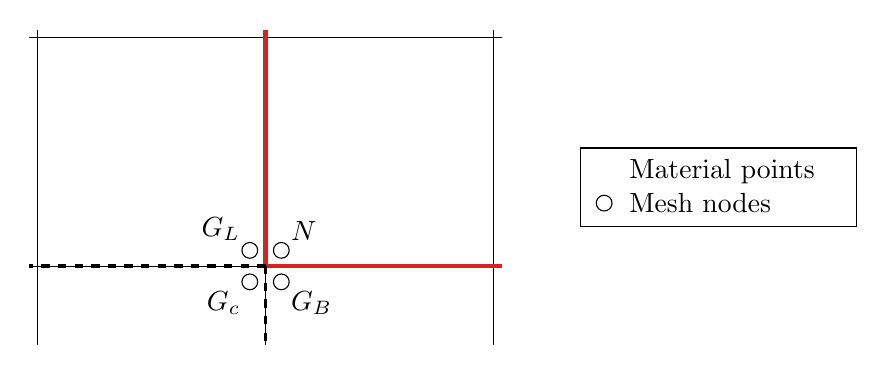
\begin{tikzpicture}
  \draw[step=2.9,black,thin] (-3.,-1.) grid (3,3.);
  \draw[ultra thick,Red] (0,3.) -- (0,0) -- (3.,0);
  % \draw[very thick,white] (0,0)--(0,-1.);
  % \draw[very thick,white] (0,0)--(-3.,-0.);
  \draw[very thick,dashed] (0,0)--(0,-1.);
  \draw[very thick,dashed] (0,0)--(-3.,-0.);
  \fill[white] (-0.2,-0.2) circle (0.1) node [below left] {$G_c$};
  \fill[white] (0.2,-0.2) circle (0.1) node [below right] {$G_B$};
  \fill[white] (-0.2,0.2) circle (0.1) node [above left] {$G_L$};
  \fill[white] (0.2,0.2) circle (0.1) node [above right] {$N$};    
  \draw[black] (-0.2,-0.2) circle (0.1) node [below left] {$G_c$};
  \draw[black] (0.2,-0.2) circle (0.1) node [below right] {$G_B$};
  \draw[black] (-0.2,0.2) circle (0.1) node [above left] {$G_L$};
  \draw[black] (0.2,0.2) circle (0.1) node [above right] {$N$};    
  \cross{0.3}{1.5};\cross{1.}{0.75};\cross{2.}{0.5};\cross{1.}{2.};
  \cross{2.5}{1.75};
  \draw (4.0,0.5) rectangle (7.5,1.5);
  \fill[white] (4.3,0.8) circle (0.1) node [right,black] {\: \text{Mesh nodes}};
  \draw[black] (4.3,0.8) circle (0.1);
  \cross{4.3}{1.2};
  \node[right] at (4.3,1.2) {\: \text{Material points}};
\end{tikzpicture}
  \caption{Corner ghost nodes in a two-dimensional DGMPM mesh.}
  \label{fig:corner_ghost}
\end{figure}
Transverse corrections further require the introduction of corner ghost nodes equivalent to finite volume corner cells \cite{Leveque}. Consider the two-dimensional case depicted in figure \ref{fig:corner_ghost} in which boundary edges are represented by red lines.
%First, boundary interfaces are extended to the corner cell (vertical and horizontal dashed lines).
First, an inverse Riemann problem is solved between the corner ghost node $G_c$ and one regular ghost node, say $G_B$, so that the stationary solution of the Riemann problem between those ghost nodes corresponds to the boundary condition holding on the vertical edge.
Second, this procedure is repeated between the corner ghost node and $G_L$ in order to enforce the boundary condition holding on the bottom boundary between them.

\begin{remark}
  \label{rq:BC_ghostnode}
  The solution of Riemann problems involving ghost nodes is made possible by extending material properties of the adjacent cell so that the characteristic structure of the solution can be computed. This implies that the deformation of interior nodes is duplicated to ghost nodes for problems such as hyperelasticity, which eigenstructure depends on the deformation gradient. Hence, for such problems ghost nodes may carry stress and strain that are not related by constitutive equations. However, the deformation gradient at ghost nodes has no physical sense and is only used to compute the correct wave speeds.
\end{remark}

\subsection{DGMPM solution scheme}
Let us assume that the vector of specific conserved quantities $\bar{\Wcb}^n$ as well as the auxiliary vector $\Qcb^n$ are known at every material points that discretize a continuum body $\Omega_0$, in a grid made of $N_{n}$ nodes at a given time $t^n$. The computational procedure followed within the DGMPM between two time steps $n$ and $n+1$ can now be derived. We consider here cases based on the use of an auxiliary vector, the others being only particular cases.
% , which requires to (i) solve the hyperbolic system \eqref{} in $\Omega$ with associated boundary conditions and (ii) update the vector $\bar{\Qcb}^n$ on material points.

The scheme has been established with a total Lagrangian formulation, therefore, the lumped mass and \textit{pseudo-stiffness} matrices $M^L_{ij}$ and $K^\alpha_{ij}$ are computed once and for all at the beginning of the calculation. The procedure then reads:
\begin{itemize}
%\item[] $\bar{\Wcb}, \:\Qcb$ known at material points
\item[(a)] The discrete equation \eqref{eq:DGMPM_discrete} and Riemann problems at cells interfaces \eqref{eq:RP_quasilinear} require a projection of fields onto the grid:
  \begin{equation}
    \label{eq:DGMPM_points2nodes}
    M^L_i \bar{\Wcb}^i = \sum_{p=1}^{N_p} S_{ip} m_p \bar{\Wcb}^p \qquad \text{and} \qquad M^L_i \vect{\Qc}^i = \sum_{p=1}^{N_p} S_{ip} m_p \vect{\Qc}^p 
  \end{equation}
  to be solved for each $\bar{\Wcb}^i$ and $\vect{\Qc}^i$ respectively. The projection of fields from particles to nodes hence follows the weighted least squares interpolation used in MPM. 
%\item[(b)] Compute time step: in the general case the tangent modulus depends on the deformation gradient as well as the waves speeds. It is therefore needed to compute the time step so that the fastest wave can at most cross the smallest cell of the mesh according to Courant condition.
\item[(b)] The specific flux vectors $\bar{\Fcb}^i_{\alpha}$ involved in the equations are computed from $\vect{\Qc}^i$ knowing $\rho_0$, thus avoiding the computation of constitutive equations.
\item[(c)] Enforcement of boundary conditions on ghost nodes.
\item[(d)] Computation of interface fluxes: 
  \begin{itemize}
  \item[1-] Build the state vectors $\vect{\Qc}_{X_N^{\pm}}$ based on $\vect{\Qc}^{i,n}$ where $i$ denotes the nodes belonging to the face on both sides of an interface.
  \item[2-] Compute the stationary solution $\Qcb^*$ by means of the approximate-state Riemann solver.
  \item[3-] Calculate the corresponding Godunov flux $\Fcb_N \(\Qcb^*\)$ by either using the DCU or the CTU approach.
  \end{itemize} 
\item[(e)] Advance solution in time by solving the discrete equation \eqref{eq:DGMPM_discrete} at each node.
\item[(f)] Back-mapping: as motivated at the end of section \ref{sec:MPM}, the nodal updated solution is projected to material points with the classical interpolation as in PIC:
  \begin{equation}
    \bar{\Wcb}^{p,n+1} = \sum_{i=1}^{N} S_{ip}\bar{\Wcb}^{i,n+1}
  \end{equation}
\item[(g)] Material point kinematics and constitutive model: The new solution $\bar{\Wcb}^{p,n+1}$ allows to increment the deformation $\vect{\varphi}(\vect{X},t)$ and to update stress components, which will be used in the auxiliary vector for the next time step, through hyperelastic constitutive equations:
  \begin{align}
    & \vect{\varphi}^{p,n+1} = \vect{X}^p + \Delta t \vect{v}^{p,n+1} \\
    & \tens{\Pi}^{p,n+1} =  \drond{\Psi}{\tens{F}}(\tens{F}^{p,n+1})
  \end{align}
  The grid may then be discarded and reconstructed and in particular by means of adaptive algorithms applied in the reference configuration, in order to improve wave front tracking in the current one.
\end{itemize}

Let's now recall or highlight significant differences between the DGMPM and the original MPM schemes. 
% Ouai ?
%First, while the DGMPM uses a classical interpolation to mapping back the updated solution to material points (step f), FLIP method and MPM require an additional time integration on material points. 
% ok
First, the use of conservation laws \eqref{eq:conservative_form} instead of the momentum equation in the weak form implies that both velocity and gradients are solved at nodes making this new approach close to finite volume methods, which provides the same order of accuracy for both fields. 
% ok
Next, since the deformation gradient is no longer calculated with shape functions gradients, the task of choosing between USF and USL algorithms vanishes. In that sense the DGMPM scheme is simpler.
At last, the solution of Riemann problems at every edges of the mesh increases computational time. Fortunately, the use of discontinuous Galerkin approximation makes this numerical method highly parallelizable \cite{Cockburn}.

The numerical scheme derived above is analyzed in terms of staiblity and convergence in the next secion.


%%% Local Variables: 
%%% mode: latex
%%% TeX-master: "../mainManuscript"
%%% End:


\section{Numerical analysis of the DGMPM}
\label{sec:DGMPM_analysis}
see Roe theorem \cite[p.417]{Toro}
\subsection{Convergence analysis}
\subsection{One-dimensional stability analysis}
Euler + RK2
\subsection{Two-dimensional stability analysis}



%%% Local Variables: 
%%% mode: latex
%%% TeX-master: "../mainManuscript"
%%% End:


\section{Conclusion}
In this chapter, the formulation of the MPM has been recalled and some drawbacks of the method when applied to hyperbolic problems have been emphasized in section \ref{sec:MPM}. It has been seen that the projection of the nodal velocity field to material points inherited from FLIP, though it reduces the numerical diffusion, introduces noise in the solution.
Hence, an alternative method using both PIC mapping procedure and Discontinuous Galerkin approximation has been proposed in section \ref{sec:DGMPM} in order to avoid spurious oscillations.
% Hence, an alternative to this mapping procedure in order to avoid numerical dissipation within the MPM without introducing numerical noise has been proposed by means of the Discontinuous Galerkin approximation in section \ref{sec:DGMPM}.
The resulting DGMPM is based on the weak form of a system of conservation laws written element by element in an arbitrary computational grid in which particles can move. Interface fluxes involved in boundary integrals of the weak form result from the solution of Riemann problems at cells interfaces computed thanks to an approximate Riemann solver (see section \ref{subsec:interface_fluxes}). This method combines thus the strength of Finite Element and Finite Volume methods.

The numerical analysis of the scheme applied to the solution of one and two-dimensional linear scalar advection equations performed in section \ref{sec:DGMPM_analysis} led to the ability to determine the maximal Courant number ensuring stability for a given discretization.
This property allows to fully exploit the ability of the method to, for instance, rebuild the grid arbitrarily by employing adaptive mesh techniques on the reference configuration in order to accurately track waves in the current one. Indeed, after such a reconstruction, the number and positions of material points in grid cells can change and one must properly adapt the CFL number so that the scheme remains stable. An advantage on the original MPM is hence highlighted since no stability condition exists for the method. It is however worth noticing that the MPM seems less dependent to the particles distribution so that the CFL is usually set to an arbitrary value ($0.5$ or $0.7$ for one and two-dimensional problems).
The DGMPM is on the other hand, characterized by a CFL number that can be set at one in particular cases.

In addition to the stability of the method, the convergence properties of the DGMPM have been compared to that of the original MPM on a one-dimensional elastic problem. 
While the MPM, as FEM, shows a second-order accuracy in velocity and first-order in stress, the DGMPM exhibits a first-order accuracy for both fields. 
The loss of accuracy has been attributed to the back-mapping used in the DGMPM and strategies to handle higher-order approximations have been proposed. 
However, the purpose of this work being the accurate capturing of waves that can be non-regular, high-order accuracy goes beyond the scope of this thesis.%is not essential for it leads to more regularity in the numerical solution.

In the following, attention is paid to the capturing of waves without oscillations unlike what has been highlighted for the MPM in section \ref{sec:MPM}. 
The object of the next chapter is the illustration of the DGMPM performances with one and two-dimensional simulations.




%%% Local Variables: 
%%% mode: latex
%%% TeX-master: "../mainManuscript"
%%% End:


%% Chapter 4: Numerical Results
\chapter{}

%% Chapter 5: Contribution to the solution of two-dimensional elastoplastic problems
%\chapter{Contribution to the solution of elastic-plastic problems in two space dimensions}
%% Faire un historique des formulations faites.
%% Formuler le problème à notre sauce et identifier les cas évoqués en intro en particularisant les modules tangents etc. a ce moment, parler des trajets de chargement et des types d'ondes

\section*{Introduction}
It has been shown throughout this manuscript that hyperbolic problems of solid mechanics are solved in a different manner depending on the numerical explicit method employed. 
In particular, irreversible deformations which are usually computed numerically based on well-known constitutive integrators, may greatly differ from one scheme to another, even for one-dimensional problems.
However, the accurate assessment of residual stresses and strains are of major importance for many industrial applications such as, among others, high-speed metal forming, crash-proof design or the study of earthquakes impact on structures.
The simulations performed in chapter \ref{chap:chap4} emphasized the improvements enabled by the knowledge of the characteristic structure of the solution of conservation laws systems, especially for elastoplastic solids.
Nevertheless, the introduction of the exact solution by means of approximate Riemann solvers is so far only carried out for one-dimensional and specific multi-dimensional loading cases for elastic-plastic solids.

The purpose of this chapter is to provide solutions and clues for future works for more general two-dimensional elastoplasticity problems under small strains. 
More information on the structure of solutions to these problems allow a better understanding of physical phenomena occuring in media on the one hand, and the ability of accurately deal with them numerically on the other hand.
The chapter is organized as follows.
A brief historical review of the solution of plastic waves in two-dimension space is made in section \ref{sec:review}.
Then, the equations of plastic flow, which characteristic analysis is carried out, are recalled in section \ref{sec:charac_plast}.
Attention is next paid in section \ref{sec:stress_paths} to the evolution of stress components through simple waves possibly arising in the solution. 
Some thus identified loading paths are finally discussed in section \ref{sec:ep_Riemman_solver} in the context of the development of dedicated approximate Riemann solvers. 

\section{Historical review}
\label{sec:review}
Until the 50s, researches on dynamic problems in elastic-plastic solids were focused on uni-axial stress or strain, pure bending or pure torsion loading conditions \cite{Taylor,vonKarman}, and were carried out for materials characterization purposes.
The first references that brought some understanding about the response of linearly hardening solids to combined shear and pressure loads are those of Rakhmatulin \cite{Rakhmatulin} and Cristescu \cite{CRISTESCU19591605}.
These early analytical investigations on plane stress impacts in the plastic regime led to the conclusion that elastic waves, as well as plastic combined-stress simple waves, can propagate in two-dimensional solids. 
While the former were well-known, the latter were shown to fall into the two \textit{fast waves} and \textit{slow waves} families.
% It has been moreover shown that the fast waves propagate faster than the plastic pressure discontinuity in uni-axial problems would, for a given compression load amplitude.
% Likewise, slow waves propa
% The maximal value of fast waves (\textit{resp. slow waves}) is higher than that of pressure (\textit{resp. shear}) plastic discontinuity occuring in one-dimensional problems, for a given compression (\textit{resp. shear}) load amplitude.

Later, Bleich and Nelson \cite{Bleich} considered superimposed plane and shear waves in an ideally elastic-plastic materials submitted to step loads.
It has then been highlighted that different loading cases yield different characteristic structures of the solution of a Picard problem, thus revealing the complexity of plastic flows in more than one dimension.
% Distinguer un peu plus ces deux contributions.
%\thomas{see \cite[p.56 pdf]{Nowacki},\cite{Goel}}. 
The same conclusions have been drawn by Clifton \cite{Clifton} for hardening materials under tension-torsion, who furthermore studied the influence of plastic pre-loading on the solution.
This contribution established the existence of loading paths through the simple waves arising from the characteristic analysis of the hyperbolic system.
Indeed, the combined-stress wave nature lies in ODEs which govern the evolution of stress components within the simple waves.
The integration of these equations of the form $d\sigma_{11}=\psi d\sigma_{12}$ allows the building of curves that connect the applied stress state of the Picard problem $(\sigma^d_{11},\sigma^d_{12})$ to the initial state of the medium.
% Indeed, the study mathematical properties of relations between stress components of the form $d\sigma_{11}=\psi d\sigma_{12}$, satisifed inside fast and slow simple waves, allows to connect the applied stress state of the Picard problem $(\sigma^d_{11},\sigma^d_{12})$ to the initial state of the medium.
It has been for instance shown that if a solid is acted upon by a traction force such that $\sigma^d_{11}=0$ and $\sigma^d_{12}$ lies outside the elastic convex, only an elastic shear discontinuity, followed by a slow simple wave, propagates.
Conversely, other loading conditions may lead to the combination of an elastic pressure discontinuity and a fast wave, possibly followed by a slow wave.
Another notable conclusion is that the combined loading paths followed inside simple waves may lead to plastic unloading, whereas only elastic unloading occurs in the one-dimensional theory.
%In addition, it is possible to meet unloading plastic simple waves with contrast to the one-dimensional theory in which the unloading waves propagate at elastic speeds (c'est pas vraiment ça attention).
%Such loading paths are supplemented by ODEs satisfied by the velocity components so that a closed form of the solution of the problem can be derived.

Experimental data collected on a thin-walled tube submitted to a dynamic tensile load \cite{Clifton_exp,Clifton_exp2} confirmed the existence of two distinct families of  simple waves, both involving combined stress paths.
Those works nevertheless exhibited some discrepancies with the theory which have been attributed to the assumption made on the von-Mises yield surface.
As a matter of fact, a constant strain region lying between the fast and slow waves that is predicted by the theory \cite{Clifton} could not be seen in experimental results.
However, by following the endochronic theory of plasticity \cite{Valanis} which does not require the introduction of a yield surface, Wu and Lin \cite{Wu_experimental} obtained numerical results that better fitted the experimental data provided by Lipkin and Clifton \cite{Clifton_exp2}.
The good agreement showed between numerical and experimental results \cite{Wu_experimental} thus confirmed the theory.

Ting and Nan \cite{Ting68} then generalized the work of Bleich and Nelson to hardening materials and Ting \cite{Ting69} widened this of Clifton to more complex loadings, that is a superimposition of one plane wave and two shear waves states.
Once again, the mathematical study of the ODE system governing the stresses evolution inside fast and slow simple waves led to the construction of loading paths in the stress space that depend on the external loads. A review of governing equations for all the cases depending on one space dimension considered above can be found in \cite{Nowacki}.

The information on characteristic structures thus provided has then be used by Lin and Ballman \cite{Lin_et_Ballman} for the development of an iterative Riemann solver.
This procedure is based on successive guesses on the stress state lying in the stationary region so that the loading paths predicted by the theory of Clifton \cite{Clifton} can be integrated numerically until convergence.
The implementation of this solver within a second-order Godunov scheme provided results that were in good agreement with the exact solutions.
Nevertheless, the theoretical investigations mentioned above restrict the development of such numerical tools to problems that depend on one space dimension.
%%
Clifton tackled the solution of plane strain problems in elastic-plastic solids by looking for bi-characteristics \cite{Clifton_thesis} in order to build finite difference schemes that account for plastic waves.
The point of view adopted here is that one can benefit from the simplifications introduced by the writing of Riemann problems in an arbitrary direction of space.
Indeed, the method of characteristics rather than the more complex method of bi-characteristics can be employed with the quasi-linear forms presented in chapter \ref{chap:chap2}.

$\newline$
On the other hand, the existence of plastic shocks in solids under the plane wave assumptions has been investigated by several authors \cite{Mandel1,Germain_shock,Mandel2,Claude}.
In those references high pressure impacts were considered so that the problem may be approximated as falling into the hydrodynamics theory.
Hence, the non-monotonic state law describing the evolution of the hydrostatic pressure is responsible for the creation of shock waves due to colliding characteristics.
%%%%%
This work gave rise to discussions on the internal structure of the shock and more precisely to the nature of the load paths followed in the infinitely thin layer in the vicinity of the shock.
%% Mandel suppose un trajet radial dans le choc et donc s'affranchit de l'analyse de la structure interne.
%% Germain utilise le travail plastic comme variable d'écrouissage. + regarde la structure interne du choc pour compléter les courbes d'hugoniot ?
%% Désaccord sur la variable d'écrouissage
%% Et puis Claude

%% Trajets radiaux + hypothèses sur l'écrouissage

% Structure interne + trajet radial de Mandel



%%% Local Variables:
%%% mode: latex
%%% TeX-master: "../mainManuscript"
%%% End:


\section{Elastic-plastic wave structure in two space dimensions}
\label{sec:charac_plast}
%% Comment the possibility of widening the approach to kinematic hardening ?
\subsection{Governing equations}
We are concerned with linear isotropic hardening materials which elastic domain is given by the von-Mises yield surface, under isothermal deformations in the linearized geometrical framework.
The balance equation of linear momentum with neglected body forces, and the geometrical balance equations are:  
\begin{equation}
  \label{eq:ch5_balance_equations}
  \left\lbrace \begin{aligned}
    %\label{eq:ch5_linear_momentum}
    & \rho \dot{\vect{v}} - \nablav \cdot \tens{\sigma} = \vect{0} \\
    %\label{eq:ch5_linear_momentum}
    &  \dot{\tens{\eps}} - \nablav \cdot \(\frac{\vect{v}\otimes \tens{I} + \tens{I} \otimes \vect{v}}{2}\) = \vect{0} 
  \end{aligned} \right.
\end{equation}
In addition, the elastic-plastic constitutive equations derived from thermodynamics in section \ref{sec:constitutive-equations} are recalled here:
\begin{subequations}
  \label{eq:ch5_plasticity_equations}
  \begin{empheq}[left=\empheqlbrace]{align}
    \label{eq:ch5_von-Mises_yield}
    & f\(\tens{\sigma},\Acb \)= \sqrt{\frac{3}{2}}\norm{\tens{s}} - \(R(p)+\sigma^y\) \equiv 0,\quad \text{with }\tens{s}=\tens{\sigma}-\frac{1}{3}\tr \tens{\sigma} \tens{I} \\
    % \label{eq:ch5_kin_hard}
    % & \tens{Y}=\frac{2}{3}C\tens{\eps}^p \\
    \label{eq:ch5_iso_hard}
    & R(p)=C \: p \\
    \label{eq:elastoplastic_tangent}
    & \tens{\dot{\sigma}}=\(\Cbb^{elast} - \beta\:\tens{s}\otimes\tens{s} \):\tens{\dot{\eps}} = \Cbb^{ep}:\tens{\dot{\eps}} \\
    \label{eq:ch5_plastic_flow}
    & \beta = \frac{6\mu^2}{3\mu +C}\times\frac{1}{\tens{s}:\tens{s}}\\
    \label{eq:ch5_EP_acoustic}
    & A_{ij}^{ep}=  A_{ij}^{elast} -  \beta (n_k s_{ki})(s_{jl}n_l)
  \end{empheq}
\end{subequations}
In the expression of von-Mises yield function \eqref{eq:ch5_von-Mises_yield}, the (positive) linear isotropic hardening law \eqref{eq:ch5_iso_hard} is considered.
Moreover, the elastoplastic acoustic tensor \eqref{eq:ch5_EP_acoustic} is decomposed as an elastic part $A_{ij}^{elast}$ and a plastic part depending on the direction of the plastic flow through the coefficient $\beta$ \eqref{eq:ch5_plastic_flow}.
%At last, the (isotropic)elasticity tensor $\Cbb$ in equation \eqref{eq:elastoplastic_tangent} can be inverted to yield the following elastic law:
By inverting the (isotropic)elasticity tensor $\Cbb$ involved in equation \eqref{eq:elastoplastic_tangent}, the following elastic law is written in the isotropic case:
\begin{equation}
  \label{eq:ch5_elastic_inverse}
  \tens{\eps}^e = \frac{1+\nu}{E} \tens{\sigma} - \frac{\nu}{E} \tr \tens{\sigma} \tens{I}
\end{equation}
with Young's modulus $E$ and Poisson's ration $\nu$.

The quasi-linear form of the sets of equations \eqref{eq:ch5_balance_equations} and \eqref{eq:ch5_plasticity_equations} in a Cartesian coordinates system and an arbitrary direction $\vect{n}$ is:
\begin{equation}
  \label{eq:ch5_quasilinear_normal}
  \Qcb_t + \Jbsf \drond{\Qcb}{x_n} = \vect{0} 
\end{equation}
where $x_n=\vect{x}\cdot\vect{n}$, $\Qcb=\matrice{\vect{v}\\ \tens{\sigma}}$, and $\Jbsf$ is the Jacobian matrix.
It has been shown in section \ref{sec:characteristic_analysis} that the $3$ eigenvalues $\omega^p$ and eigenvectors $\vect{l}^p$ of the acoustic tensor lead to $6$ left characteristic fields of the Jacobian matrix $\{c_K;\Lcb^K\}$ according to:
\begin{equation}
  \label{eq:ch5_left_eigenfields}
  \left\lbrace \pm \sqrt{\frac{\omega_p}{\rho}} ; \quad \[\: \pm \rho\sqrt{\frac{\omega_p}{\rho}} \vect{l}^p , -\vect{l}^p\otimes \vect{n} \:\]  \right\rbrace ,\quad p=1,2,3
\end{equation}
In addition, three independent left eigenvectors associated to the zero eigenvalue of system \eqref{eq:ch5_quasilinear_normal}, which is of multiplicity $3$, are found by solving:
\begin{equation}
  \label{eq:ch5_null_eigen}
  \tens{\sigma}^K:\(\Cbb^{ep}\cdot  \vect{n}\) =\vect{0},\quad K=1,2,3
\end{equation}

The present formulation differs from those of \textsc{Bleich} \cite{Bleich}, \textsc{Clifton} \cite{Clifton}, and hence these of \textsc{Ting} and \textsc{Nan} \cite{Ting68} and \textsc{Ting} \cite{Ting69}, in that equation  \eqref{eq:ch5_quasilinear_normal} is based on the elastoplastic stiffnesses rather than softenesses.
As a consequence, it will be seen in what follows that the equations can be easily specialized to plane strain and plane stress cases.
%In what follows, the above equations are specified to plane strain and plane stress cases.
\subsection{Problems in two space dimensions}
We now focus on the solid domain $x_1 \times x_2 \times x_3 \in [0,\infty[ \times [-h,h] \times [-e,e]$ in a Cartesian coordinates system, where $e$ and $h$ are arbitrary lengths.
%The solid is subject in the plane $x_1=0$ to a traction force $\vect{T}^1$ restricted to the $(\vect{e}_1,\vect{e}_2)$ plane, that is $T_3=0$.
It is assumed that all quantities depend solely on $x_1$ and $x_2$ except the velocity component $v_3$ that may depend on $x_3$.
In particular, it is the case for $e \ll h$.

The solid is under plane strain conditions, that is $\tens{\eps}\cdot\vect{e}_3=\vect{0}$, if the velocity $\vect{v}$ does not depend on $x_3$ and if $v_3$ vanishes.
Thus, combining the additive partition of the infinitesimal strain tensor: $\tens{\eps}=\tens{\eps}^e+\tens{\eps}^p$, with the elastic law \eqref{eq:ch5_elastic_inverse} and the kinematic condition $\eps_{33}=0$, one gets:
\begin{equation}
  \label{eq:plane_strain_stress33}
  \sigma_{33}=\nu\(\sigma_{11}+\sigma_{22}\) - E\eps^p_{33}
\end{equation}
Hence, the quasi-linear form \eqref{eq:ch5_quasilinear_normal} reduces for plane strain problems to a system of dimension $5$ with unknowns $v_1,v_2, \sigma_{11},\sigma_{12}$, and $\sigma_{22}$.


Alternatively, a plane stress state ($\tens{\sigma}\cdot\vect{e}_3=\vect{0}$) is assumed if the planes $x_3=\pm h$ are traction free and $e\ll h$.
As a result, the stress component $\sigma_{33}$ can be removed from the system \eqref{eq:ch5_quasilinear_normal}.
Nevertheless, the tangent modulus must account for the vanishing out-of-plane stress component.
Specialization of equation \eqref{eq:elastoplastic_tangent} to $\sigma_{33}$ yields:
\begin{equation*}
  \dot{\sigma}_{33}=C^{ep}_{33ij} \dot{\eps}_{ij} =0
\end{equation*}
from which one writes:
\begin{equation*}
  C^{ep}_{3333} \dot{\eps}_{33} = - C^{ep}_{33ij}\dot{\eps}_{ij} \quad i,j=\{1,2\}
\end{equation*}
Hence, the constitutive equations are rewritten by means of a two-dimensional tangent modulus $\widetilde{\Cbb}^{ep}$:
\begin{equation}
  \label{eq:CP_constitutive}
  \dot{\sigma}_{ij}=C^{ep}_{ijkl} \dot{\eps}_{kl} - \frac{C^{ep}_{ij33}C^{ep}_{33kl}}{C^{ep}_{3333}}\dot{\eps}_{kl}= \widetilde{C}^{ep}_{ijkl} \dot{\eps}_{kl}\qquad i,j,k,l=\{1,2\} 
\end{equation}
The characteristic structure of the problem is then given by this of the associated acoustic tensor $\tens{\widetilde{A}}^{ep}=\vect{n}\cdot\widetilde{\Cbb}^{ep}\cdot \vect{n}$.

The removal of $\sigma_{33}$ from system \eqref{eq:ch5_quasilinear_normal} for both plane strains and plane stresses allows to solve the problem in a two-dimensional setting.
Then, generically denoting the acoustic tensor by $\tens{A}$, the characteristic structures are given by the eigenvalues:
\begin{subequations}
  \begin{alignat}{1}
    \label{eq:ch5_eigenAcc1}
    &\omega_1 = \frac{1}{2}\(A_{11}+A_{22} + \sqrt{(A_{11}-A_{22})^2+{4A_{12}}^2}\) \\
    \label{eq:ch5_eigenAcc2}
    &\omega_2 = \frac{1}{2}\(A_{11}+A_{22} - \sqrt{(A_{11}-A_{22})^2+{4A_{12}}^2}\)     
  \end{alignat}
\end{subequations}
and the associated eigenvectors:
\begin{equation}
  \label{eq:ch5_eigenvectAcc}
   \vect{l}^1=[ A_{22}-  \omega_1 \:,\: -A_{12}] \qquad ;\qquad  \vect{l}^2=[ -A_{12} \:,\:A_{11}- \omega_2 ]
\end{equation}
From equation \eqref{eq:ch5_left_eigenfields}, we see that two families of waves with celerities $c_f=\pm \sqrt{\omega_1/\rho}$ and $c_s = \pm \sqrt{\omega_2/\rho}$ may travel in the domain.
Those waves are respectively referred to as fast and slow waves.
Note that subtracting equations \eqref{eq:ch5_eigenAcc1} and \eqref{eq:ch5_eigenAcc2} leads to:
\begin{equation}
  \label{eq:diff_celerities}
  \rho c_f^2 - \rho c_s^2 = \sqrt{(A_{11}-A_{22})^2+{4A_{12}}^2} \geq 0
\end{equation}
Hence, the characteristic speed associated to fast waves is always greater than of equal to that of slow waves.

The four left eigenfields of the Jacobian matrix thus read:
\begin{subequations}
  \begin{alignat}{1}
    \label{eq:ch5_Jac_eigenfield_fast}
    &\left\lbrace \pm c_f ; \quad \Lcb^{c_f^\pm}=\[\: \pm \rho c_f \vect{l}^1 , -\vect{l}^1\otimes \vect{n} \:\]  \right\rbrace \\
  \label{eq:ch5_Jac_eigenfield_slow}
    &\left\lbrace \pm c_s ; \quad \Lcb^{c_s^\pm}=\[\: \pm \rho c_s \vect{l}^2 , -\vect{l}^2\otimes \vect{n} \:\]  \right\rbrace
  \end{alignat}
\end{subequations}
where $\Lcb^{c_f^+}$ and $\Lcb^{c_f^-}$ are associated to the right-going and left-going fast waves respectively.
The same goes for $\Lcb^{c_s^+}$ and $\Lcb^{c_s^-}$.
Furthermore, one stationary wave associated to the zero eigenvalue of the Jacobian matrix, and which left eigenvector satisfies equation \eqref{eq:ch5_null_eigen}, has to be added:
\begin{equation}
  \label{eq:ch5_null_left_eigen}
  {\Lcb^0}^T = \matrice{v_1^0 \\[5.pt] v_2^0 \\[5.pt] \sigma_{11}^0 \\[5.pt] \sigma^0_{22} \\[5.pt] \sigma^0_{12} }= \matrice{0 \\[5.pt] 0 \\[5.pt] \(C_{121i}C_{222j}-C_{221i}C_{122j}\)n_in_j \\[5.pt] \(C_{111i}C_{122j}-C_{112i}C_{121j}\)n_in_j \\[5.pt] \(C_{112i}C_{221j}-C_{111i}C_{222j}\)\frac{n_in_j}{2}} = \matrice{0 \\ 0 \\ \alpha_{11} \\ \alpha_{22} \\ \alpha_{12} }
\end{equation}
with $\Cbb=\Cbb^{ep}$ for plain strain and $\Cbb=\widetilde{\Cbb}^{ep}$ for plane stress.
%In particular, $\Cbb$ reduces to the elastic stiffness tensor when no plastic flow occurs so that the characteristic structure involves the speeds of elastic pressure waves $c_1$ and shear waves $c_2$. 

It has been seen in section \ref{sec:SVK_solution} that the solution of non-linear problems may contain shock and/or simple waves.
Nevertheless, we restrict here to simple waves by assuming that: (i) the characteristic speeds satisfy $c_1 \geq c_f \geq c_2 \geq c_s $, where $c_1$ and $c_2$ are the speeds of elastic pressure and shear discontinuities respectively; (ii) $c_f$ and $c_s$ monotonically decrease with the hardening of the material; (ii) the computational domain is in an initial natural, plastic strain free state.

The characteristic equations $\Lcb^K \cdot d\Qcb = 0$ are then written:
\begin{subequations}
  %\label{eq:ch5_ODEs}
  \begin{alignat}{3}
    \label{eq:charac_fr}
    & \rho c_f \vect{l}^1 \cdot d\vect{v} - l^1_i n_j d\sigma_{ij} =0 \qquad && \text{along }\: dx/dt = c_f\\
    \label{eq:charac_fl}
    -& \rho c_f \vect{l}^1 \cdot d\vect{v} - l^1_i n_j d\sigma_{ij} =0 \qquad && \text{along }\: dx/dt = - c_f \\
    \label{eq:charac_sr}
    & \rho c_s \vect{l}^2 \cdot d\vect{v} - l^2_i n_j d\sigma_{ij} =0 \qquad  && \text{along }\: dx/dt =  c_s \\
    \label{eq:charac_sl}
    -& \rho c_s \vect{l}^2 \cdot d\vect{v} - l^2_i n_j d\sigma_{ij} =0 \qquad  && \text{along }\: dx/dt = - c_s \\
    \label{eq:charac_contact}
    &\alpha_{11}d\sigma_{11} + \alpha_{12}d\sigma_{12} + \alpha_{22}d\sigma_{22}=0 \qquad && \text{along }\: dx/dt =0 
  \end{alignat}
\end{subequations}
Integration of equations \eqref{eq:charac_fr} to \eqref{eq:charac_contact} leads to integral curves through simple waves in which several stress components vary, hence the name of combined-stress simple waves \cite{CRISTESCU19591605}.
Following \cite{Clifton}, the method of characteristic is applied by combining equations \eqref{eq:charac_fr} to \eqref{eq:charac_contact}.
\begin{figure}[h!]
  \centering
  \subcaptionbox{Slow simple wave \label{subfig:slowWave}}{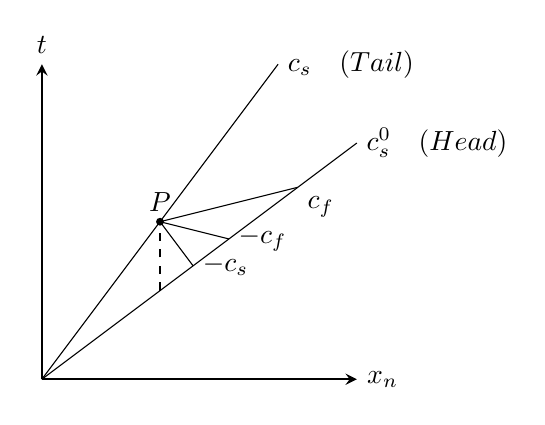
\begin{tikzpicture}[scale=1.,>=stealth] 
  \newcommand\shift{5.}
  %% Slow
  \draw[thick,->] (0,0) -- (4.,0) node[right] {$x_n$};
  \draw[thick,->] (0,0) -- (0.,4) node[above] {$t$};
  % Slope = 0.75
  \draw (0,0) -- (4,3.) node [right] {$c_s^0 \quad (Head)$};
  % Slope = 4./3.
  \draw (0,0) -- (3.,4.) node [right] {$c_s \quad (Tail)$};

  \fill[black] (1.5,1.5*4./3.) circle (0.05) node [above] {$P$};
  %% Other characteristics
  % stationary
  \draw[dashed] (1.5,0.75*1.5) -- (1.5,1.5*4./3.);
  % fast plus (slope =+-0.25)
  \newcommand\px{1.5}
  \newcommand\py{1.5*4./3.}
  \draw (2.*\py-0.5*\px,1.5*\py-3.*\px/8.) node [below right] {$c_f$}-- (1.5,1.5*4./3.) ;
  % fast minus
  \draw (\py+0.25*\px,0.75*\py+3.*\px/16.) node [right] {$-c_f$} -- (1.5,1.5*4./3.) ;
  % slow minus (slope=-4./3.)
  \draw (12.*\py/25.+16.*\px/25.,9.*\py/25.+36.*\px/75.) node [right] {$-c_s$} -- (1.5,1.5*4./3.) ;
\end{tikzpicture}


%%% Local Variables:
%%% mode: latex
%%% TeX-master: "../../mainManuscript"
%%% End:
} \qquad
  \subcaptionbox{Fast simple wave \label{subfig:fastWave}}{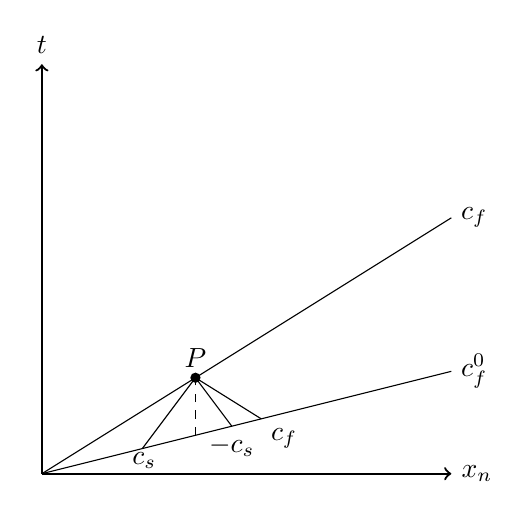
\begin{tikzpicture}[scale=1.3] 
  \newcommand\shift{5.}
  %% Fast
  \draw[thick,->] (0+\shift,0) -- (4.+\shift,0) node[right] {$x_n$};
  \draw[thick,->] (0+\shift,0) -- (0.+\shift,4) node[above] {$t$};
  % Slope = 0.25
  \draw (0+\shift,0) -- (4+\shift,1.) node [right] {$c_f^0$};
  % Slope = 5./8.
  \draw (0+\shift,0) -- (4+\shift,2.5) node [right] {$c_f$};
  
  \fill[black] (1.5+\shift,1.5*5./8.) circle (0.05) node [above] {$P$};
  %% Other characteristics
  \newcommand\pxx{1.5}
  \newcommand\pyy{1.5*5./8.}
  % stationary
  \draw[dashed] (1.5+\shift,1.5/4.) -- (\pxx+\shift,\pyy);
  % fast minus
  \draw (8.*\pyy/7.+5.*\pxx/7.+\shift,2.*\pyy/7.+10.*\pxx/56.) node [below right] {$c_f$}-- (\pxx+\shift,\pyy);
  % slow plus
  \draw (-12.0*\pyy/13.+16.*\pxx/13.+\shift,-3.*\pyy/13.+4.*\pxx/13.) -- (\pxx+\shift,\pyy);
  \node at (-12.0*\pyy/13.+16.*\pxx/13.+\shift+0.02,-3.*\pyy/13.+4.*\pxx/13.-0.12) {$c_s$};
  % slow minus
  \draw (12.0*\pyy/19.+16.*\pxx/19.+\shift,3.*\pyy/19.+4.*\pxx/19.)node [below] {$-c_s$} -- (\pxx+\shift,\pyy);
\end{tikzpicture}


%%% Local Variables:
%%% mode: latex
%%% TeX-master: "../../mainManuscript"
%%% End:
}
  \caption{The method of characteristics through slow and fast simple waves in the $(x_n,t)$ plane.}
  \label{fig:ch5_charac_method}
\end{figure}
The approach consists in tracing every characteristics from some downstream point of a wave where the state vector $\Qcb$ is known, to an upstream point where the solution is seeked. Figures \ref{fig:ch5_charac_method}\subref{subfig:slowWave} and \ref{fig:ch5_charac_method}\subref{subfig:fastWave} schematically illustrate the method for slow and fast simple waves in which the state is known along the head wave and is looked for at point $P$ lying on the tail wave. 
The integral curves through slow and fast simple waves are derived in the next section.

\subsection{Integral curves through simple waves}
The right-going slow waves are first looked at by adding equations \eqref{eq:charac_fr} and \eqref{eq:charac_fl}:
\begin{equation}
  l_i^1 n_j d\sigma_{ij}=0
\end{equation}
Given the geometry of the problem, the vector $\vect{n}$ may be reduced to $\vect{e}_1$ or $\vect{e}_2$.
It therefore comes out:
%In particular, for a vector $\vect{n}$ that is restricted to the axis of the $(\vect{e}_1,\vect{e}_2)$ plane, one gets:
\begin{subequations}
  \begin{alignat}{2}
    \label{eq:sigSlow_n=e1}
    & d\sigma_{11} = - \frac{l^1_2}{l_1^1} d\sigma_{12} = \psi^s_{1}d\sigma_{12} && \qquad \text{for } \:\vect{n}=\vect{e}_1 \\
    \label{eq:sigSlow_n=e2}
    & d\sigma_{22}=- \frac{l_1^1}{l_2^1}  d\sigma_{12} = \psi^s_{2}d\sigma_{12} && \qquad \text{for } \:\vect{n}=\vect{e}_2
  \end{alignat}
\end{subequations}
where $\psi^s_1$ and $\psi^s_2$ are functions of all components of $\tens{\sigma}$. 
Moreover, the $s$ and $f$ superscripts stand for slow and fast waves respectively in the remainder of the manuscript.
With the above equations, the characteristic equation related to the contact wave \eqref{eq:charac_contact} reads:
%Next, the characteristic equation related to the contact wave \eqref{eq:charac_contact} yields:
\begin{subequations}
  \begin{alignat}{2}
    \label{eq:sigContact_n=e1}
    & d\sigma_{22} = -\frac{\psi^s_{1}\alpha_{11}+\alpha_{12}}{\alpha_{22}}d\sigma_{12} && \qquad \text{for } \:\vect{n}=\vect{e}_1 \\
    \label{eq:sigContact_n=e2}
    & d\sigma_{11}= -\frac{\psi^s_{2}\alpha_{22}+\alpha_{12}}{\alpha_{11}} d\sigma_{12} && \qquad \text{for } \:\vect{n}=\vect{e}_2
  \end{alignat}
\end{subequations}
The sets of equations \eqref{eq:sigSlow_n=e1}-\eqref{eq:sigContact_n=e1} and \eqref{eq:sigSlow_n=e2}-\eqref{eq:sigContact_n=e2} show the combined-stress nature of slow simple waves.
% Hence, one stress component may be used as a driving parameter for the two others, as it is the case for $\sigma_{12}$ in equations \eqref{eq:sigSlow_n=e1}, \eqref{eq:sigSlow_n=e2}, \eqref{eq:sigContact_n=e1} and \eqref{eq:sigContact_n=e2}.
On the other hand, the subtraction of equations \eqref{eq:charac_fr} and \eqref{eq:charac_fl} leads to:
\begin{equation*}
  dv_1 = \psi^s_{1}dv_2 = \frac{1}{\psi^s_2}dv_2
\end{equation*}
which, once combined with equations \eqref{eq:sigSlow_n=e1}-\eqref{eq:sigSlow_n=e2} and introduced in \eqref{eq:charac_sl}, yields after simplifications:
\begin{subequations}
  \begin{alignat}{2}
    \label{eq:vSlow_n=e1}
    & dv_1 = -\frac{d\sigma_{11}}{\rho c_s^2} \quad ;\quad  dv_2 = -\frac{d\sigma_{12}}{\rho c_s^2} \qquad & \text{for } \vect{n}=\vect{e}_1\\
    \label{eq:vSlow_n=e2}
    & dv_1 = -\frac{d\sigma_{12}}{\rho c_s^2} \quad ;\quad  dv_2 = -\frac{d\sigma_{22}}{\rho c_s^2} \qquad & \text{for } \vect{n}=\vect{e}_2
  \end{alignat}
\end{subequations}

\begin{remark}
  The integral curves through a left-going slow wave result from the combination of equations \eqref{eq:sigSlow_n=e1}-\eqref{eq:sigSlow_n=e2} introduced in \eqref{eq:charac_sr} rather than \eqref{eq:charac_sl}.
  Therefore, the only difference lies in the signs in equations \eqref{eq:vSlow_n=e1} and \eqref{eq:vSlow_n=e2}
\end{remark}

Similar results are obtained for right-going fast simple waves by using $\vect{l}^2$ instead of $\vect{l}^1$ and $c_f$ rather than $c_s$.
%However, the integral curves involve $\vect{l}^2$ and $c_f$ instead of $\vect{l}^1$ and $c_s$. 
Hence, the evolution in slow and fast waves is governed by the \textit{loading functions}:
\begin{equation}
  \label{eq:loading_func}
  \psi^s_{1}=- \left.\frac{l^1_2}{l_1^1}\right\rvert_{\vect{n}=\vect{e}_1}\quad ,\quad  \psi^s_{2}=- \left.\frac{l_1^1}{l_2^1}\right\rvert_{\vect{n}=\vect{e}_2} \quad ,\quad \psi^f_1=-\left.\frac{l_2^2}{l_1^2}\right\rvert_{\vect{n}=\vect{e}_1} \quad ,\quad \psi^f_2=-\left.\frac{l_1^2}{l_2^2}\right\rvert_{\vect{n}=\vect{e}_2}
\end{equation}
The equations satisfied across right-going slow and fast simple waves are summarized in table \ref{tab:simpleWavesEquations}.
\begin{table}[h!]
  \centering
  \begin{tabular}{cc|ccN}
    \hline
    \multicolumn{2}{c}{Right-going slow wave} \vline& \multicolumn{2}{c}{Right-going fast wave} & \\
    $\vect{n}=\vect{e}_1$ & $\vect{n}=\vect{e}_2$ & $\vect{n}=\vect{e}_1$ & $\vect{n}=\vect{e}_2$&\\
    \hline
    \hline
    $dv_1 = -\frac{d\sigma_{11}}{\rho c_s^2}$ &  $dv_1 = -\frac{d\sigma_{12}}{\rho c_s^2}$ &$dv_1 = -\frac{d\sigma_{11}}{\rho c_f^2}$ &  $dv_1 = -\frac{d\sigma_{12}}{\rho c_f^2}$ &\\ [8pt]
    $dv_2 = -\frac{d\sigma_{12}}{\rho c_s^2}$ & $dv_2 = -\frac{d\sigma_{22}}{\rho c_s^2}$ & $dv_2 = -\frac{d\sigma_{12}}{\rho c_f^2}$ & $dv_2 = -\frac{d\sigma_{22}}{\rho c_f^2}$& \\ [8pt]
    $d\sigma_{11} = \psi^s_{1}d\sigma_{12}$&$d\sigma_{11}= -\frac{\psi^s_{2}\alpha_{22}+\alpha_{12}}{\alpha_{11}} d\sigma_{12}$ &  $d\sigma_{11} = \psi^f_{1}d\sigma_{12}$&$d\sigma_{11}= -\frac{\psi^f_{2}\alpha_{22}+\alpha_{12}}{\alpha_{11}} d\sigma_{12}$ & \\[8pt]
    $d\sigma_{22} = -\frac{\psi^s_{1}\alpha_{11}+\alpha_{12}}{\alpha_{22}}d\sigma_{12}$ & $d\sigma_{22}= \psi^s_{2}d\sigma_{12}$ & $d\sigma_{22} = -\frac{\psi^f_{1}\alpha_{11}+\alpha_{12}}{\alpha_{22}}d\sigma_{12}$ & $d\sigma_{22}= \psi^f_{2}d\sigma_{12}$ & \\[8pt]
    % & & \\
    % & & \\    
    \hline
\end{tabular}
%%% Local Variables:
%%% mode: latex
%%% TeX-master: "../manuscript"
%%% End:

  \caption{Summary of the ODEs satisfied inside right-going slow and fast simple waves.}
  \label{tab:simpleWavesEquations}
\end{table}

The integration of equations gathered in table \ref{tab:simpleWavesEquations} should provide the complete solution of a given problem by means of integral curves or loading paths.
For instance, the velocity resulting from the passage of right-going waves in the direction $\vect{e}_1$ obeys:
\begin{equation}
  \label{eq:integral_example}
  v_1 = v_1^0 - \int_{\tens{\sigma}^0}^{\tens{\sigma}} \frac{d \sigma_{11}}{\rho c^2} \quad ;\quad v_2 = v_2^0 - \int_{\tens{\sigma}^0}^{\tens{\sigma}} \frac{d \sigma_{12}}{\rho c^2}
\end{equation}
where the zero superscript denotes the downstream state.
Nevertheless, \textsc{Clifton} \cite{Clifton} emphasized that depending on the loading conditions, only one simple waves or both may arise in the solution.
Therefore, it is crucial to identify the stress path followed to properly compute integrals \eqref{eq:integral_example}.
%It is thus important to qualify the stress paths through fast and slow waves in order to properly define the upper bound of the integrals of the form \eqref{eq:integral_example}.
This is the purpose of the next section.



%%% Local Variables:
%%% mode: latex
%%% TeX-master: "../mainManuscript"
%%% End:


\section{Loading paths through simple waves}
\label{sec:stress_paths}
% On ne regarde qu'une dimension spatiale en faisant des hypothèse sur les champs alors que nous on se limite à une direction particulière $\vect{n}$.
% En plus, on se limite à l'étude d'ondes simples alors que des chocs peuvent exister (voir Mandell car il semble y etre démontré que les shock n'arrivent que pour $\tau=0$).
% Il y a la question des vitesses charactéristiques plastiques... sont-elles collées aux vitesses élastiques ?
% dependance des vitesses caractéristiques à l'angle entre la direction principale de sigma et la direction de propagation, c'est dit dans la thèse de Clifou en page 90.

\subsection{Properties of the loading paths}
The stress paths followed within slow and fast simple waves are governed by the mathematical properties of the loading functions \eqref{eq:loading_func}.
Before specializing the discussion to plane stress and plane strain cases, some general properties holding regardless of the loading conditions are highlighted.
%The analysis is here carried out for the special case $\vect{n}=\vect{e}_1$, similar results being obtained for the other situation $\vect{n}=\vect{e}_2$.

First, the functions satisfy the orthogonality properties: $\psi^s_1\psi^f_1=-1$ and $\psi^s_2\psi^f_2=-1$.
Indeed, considering the left eigenvectors of the acoustic tensor given in equation \eqref{eq:ch5_eigenvectAcc}, the product $\psi^s_1\psi^f_1$ reads:
\begin{equation*}
  \psi^s_1\psi^f_1 = \frac{l^1_2}{l^1_1}\: \frac{l_2^2}{l^2_1} = \frac{(A_{11}-\omega_2)A_{12}}{(A_{22}-\omega_1)A_{12}}
\end{equation*}
Introduction of the expressions of eigenvalues $\omega_i$ from equations \eqref{eq:ch5_eigenAcc1} and \eqref{eq:ch5_eigenAcc1} further leads to:
\begin{equation*}
  \psi^s_1\psi^f_1 = \frac{A_{11} -A_{22} +\sqrt{(A_{11} -A_{22} )^2 + 4A_{12}^2 }}{A_{22} -A_{11} -\sqrt{(A_{11} -A_{22} )^2 + 4A_{12}^2 }}=-1
\end{equation*}
or equivalently, $\vect{l}^1 \cdot \vect{l}^2=0$.
%as expected by the symmetry of $\tens{A}$.
This orthogonality has already been noticed for particular plane strain and plane stress cases \cite{Clifton,Ting68}. % but now obviously appears as true for all problems in two space dimensions.
However, the eigenvectors of symmetric second-order tensors all satisfy this property in such a way that it is valid for all problems in two space dimensions.
As a result, the study can be restricted to one function in each direction, say $\psi_1^s$ and $\psi_2^s$.

Second, if the function $\psi_1^s$ vanishes at some point of the stress space, the projection of the loading path followed inside a slow wave in the $(\sigma_{11},\sigma_{12})$ plane is vertical according to the ODE \eqref{eq:sigSlow_n=e1}.
Conversely, if $\psi_1^s\rightarrow \infty$, the loading path is horizontal in the $(\sigma_{11},\sigma_{12})$ plane.
%Looking for vanishing $\psi^f_1$ or $1/\psi^f_1$ amounts to finding roots of the components of $\vect{l}^2$:
These situations respectively correspond to:
\begin{subequations}
  \begin{alignat}{1}
    \label{eq:first_root}
    \psi_1^s = 0   & \Leftrightarrow A_{12} =0  \\
    \label{eq:second_root}
    \psi_1^s \rightarrow \infty & \Leftrightarrow A_{22} -\omega_1 =0
  \end{alignat}
\end{subequations}
In particular, if $A_{12}=0$ the second equation reads:
\begin{equation}
  A_{22} -\omega_1 = \frac{1}{2}\(A_{22} -A_{11} -\sqrt{(A_{11} -A_{22} )^2 + 4A_{12}^2 }\) = -\left\langle A _{11}-A _{22}  \right\rangle
\end{equation}
where $\left\langle \bullet \right\rangle$ denotes the positive part operator.
Hence, if $A_{12} =0$ and $A_{11} \neq A_{22} $, one has $\psi^s_1 =0$ and hence $\psi^f_1 \rightarrow -\infty $.
If moreover $A_{11}  = A_{22} $, both components of the eigenvectors vanish and the functions $\psi^s_1$ and $\psi^f_1$ are undetermined.
At last, it follows from equation \eqref{eq:diff_celerities} that the simultaneous satisfaction of conditions \eqref{eq:first_root} and \eqref{eq:second_root} leads to characteristic speeds of simple waves that are identical. Hence, the situation $c_f=c_s$ corresponds to a loss of hyperbolicity of the system.
% Hence, if $A_{12} =0$ and $A_{11} \neq A_{22} $, one has $\psi^s_1 =0$ and $\psi^f_1 \rightarrow \infty $, so that the stress path in the ($\sigma_{11},\sigma_{12}$) plane are vertical (\textit{resp. horizontal}) through a slow (\textit{resp. fast}) wave. 

Analogously, the function $\psi_2^s$ is such that:
\begin{subequations}
  \begin{alignat}{1}
    \label{eq:first_root_psi2cp}
    \psi_2^s \rightarrow \infty  & \Leftrightarrow A_{12} =0  \\
    \label{eq:second_root_psi2cp}
    \psi_2^s =0 & \Leftrightarrow A_{22} -\omega_1 =0
  \end{alignat}
\end{subequations}
Therefore, if both conditions \eqref{eq:first_root_psi2cp} and \eqref{eq:second_root_psi2cp} are satisfied, the system is no longer hyperbolic with characteristic speeds of fast and slow waves that are identical.

According to the ODEs of table \ref{tab:simpleWavesEquations}, the particular values of the loading functions $\psi_i^{s,f}$ through the simple waves propagating in direction $\vect{e}_i$ for $i=\{1,2\}$, provide information about the loading paths in stress space.
First, $\psi_i =0$ leads to $d\sigma_{ii}=0$ (no sum on $i$) so that the longitudinal stress is constant within the simple wave.
Conversely, with loading functions tending to infinity, the stress $\sigma_{12}$ does not vary.
Notice that the coefficients $\alpha_{ij}$ of the left eigenvector of the Jacobian matrix associated to the zero eigenvalue \eqref{eq:ch5_null_left_eigen} also have to be regarded.
Nevertheless, those terms resulting from products of the components of the elastoplastic tangent modulus have complex expressions and are assumed to have non-zero values in the remainder of the manuscript.

The above discussions are now specified to plane strain and plane stress, for which loading conditions leading to $A_{12} =0$ and $A _{11}-A _{22}=0$ are identified.



\subsection{The plane strain case}
The case of plane strain is first considered by using the elastoplastic tangent modulus so that the components of the acoustic tensor for $\vect{n}=\vect{e}_1$ read:
%The elastoplastic tangent modulus under consideration is now that given in equation \eqref{eq:elastoplastic_tangent}, so that the components of the acoustic tensor for $\vect{n}=\vect{e}_1$ read: 
\begin{subequations}
  \begin{alignat}{1}
    \label{eq:DP_A11}
    & A_{11}^{ep}= C_{1111}^{ep} = \lambda + 2\mu -\beta s_{11}^2 \\
    \label{eq:DP_A22}
    & A_{22}^{ep}= C_{2121}^{ep}= \mu -\beta s_{12}^2 \\
    \label{eq:DP_A12}
    & A_{12}^{ep}= C_{1121}^{ep}=-\beta s_{11}s_{12}
  \end{alignat}
\end{subequations}
The associated eigenvalues are then:
\begin{subequations}
  \label{eq:eigen_acc_DP}
  \begin{alignat}{1}
    \label{eq:eigen_acc_DP1}
    & \rho c_s^2 = \frac{1}{2}\( \lambda +3\mu -\beta (s_{11}^2+ s_{12}^2) - \sqrt{(\lambda + \mu -\beta (s_{11}^2-s_{12}^2) )^2 +4(\beta s_{11}s_{12})^2} \) \\
    \label{eq:eigen_acc_DP2}
    & \rho c_f^2 = \frac{1}{2}\( \lambda +3\mu -\beta (s_{11}^2+ s_{12}^2) + \sqrt{(\lambda + \mu -\beta (s_{11}^2-s_{12}^2) )^2 +4(\beta s_{11}s_{12})^2}  \)
  \end{alignat}
\end{subequations}
Subtracting equations \eqref{eq:DP_A11} and \eqref{eq:DP_A22}, one gets: $A_{11}^{ep}-A_{22}^{ep}= \lambda + \mu -\beta \(s_{11}^2-s_{12}^2\)$.
Hence, the equation $A_{11}^{ep}-A_{22}^{ep}=0$ admits a set of solutions in the deviatoric stress space.
On the other hand, we see from equation \eqref{eq:DP_A12} that $A_{12}^{ep}$ vanishes for $s_{12}=0$ and $s_{11}=0$.
% Recall that $A^{ep}_{12}=0$ leads to vertical and horizontal loading paths across slow and fast waves respectively. 
Each solution is studied in more details below.

%% Sign of one of the functions psi... but not used afterwards
% We first study the sign of the functions $\psi^f$ by noticing that $\mu=\rho c_2^2$ so that $A_{22}^{ep}$ may be rewritten to yield:
% \begin{equation*}
%   \psi^f = -\frac{A_{12}^{ep}}{A_{22}-\rho c_f^2}= -\frac{\beta s_{11}s_{12}}{\rho c_f^2-\rho c_2^2 +\beta s_{12}^2 }
% \end{equation*}
% Since the denominator is positive for $c_f \geq c_2$, it comes out that $\sign (\psi^f) = - \sign(s_{12}) \sign(s_{11})$. Moreover, two roots of the loading function $\psi^f$ can be identified.

\paragraph*{Condition $s_{12}=0$:} 
According to equations \eqref{eq:eigen_acc_DP1} and \eqref{eq:eigen_acc_DP2}, the eigenvalues of the acoustic tensor become:
\begin{align*}
  & \rho c_s^2 = \frac{1}{2}\( \lambda +3\mu -\beta s_{11}^2 - \abs{\lambda + \mu -\beta s_{11}^2 } \) \\
  & \rho c_f^2 = \frac{1}{2}\( \lambda +3\mu -\beta s_{11}^2 + \abs{\lambda + \mu -\beta s_{11}^2 } \)
\end{align*}
Thus, assuming that $\beta s_{11}^2 < \lambda + \mu$, the expression further reduces to:
\begin{align*}
  & \rho c_s^2 = \mu \\
  & \rho c_f^2 = \lambda +2\mu -\beta s_{11}^2 
\end{align*}
The characteristic speed of slow waves therefore identifies with this of elastic shear waves for plane strain $c_s=c_2=\sqrt{\mu/\rho}$. 
If conversely $ \lambda + \mu - \beta s_{11}^2$ is negative, the characteristic speeds read: 
\begin{align*}
  & \rho c_s^2 = \lambda +2\mu -\beta s_{11}^2  \\
  & \rho c_f^2 =  \mu 
\end{align*}
As a result, in that case it is the celerity of fast waves which reduces to that of elastic shear waves.
Note however that for the characteristic speed of slow waves remains real, the stress $s_{11}$ must satisfy $\beta s_{11}^2 < \lambda +2\mu$.
At last, the equality $\beta s_{11}^2 = \lambda + \mu$ leads to $A_{11}^{ep}-A_{22}^{ep}=0$ and hence, to undetermined loading functions. 
%% Set of admissible values for s11 (depends on s itself)
% It then appears that the values of $s_{11}$ ensuring hyperbolicity of the system are:
% \begin{equation}
%   s_{11} \in ]-\infty,-\sqrt{\frac{\lambda + \mu}{\beta}}[\: \cup\: ]-\sqrt{\frac{\lambda + \mu}{\beta}},\sqrt{\frac{\lambda + \mu}{\beta}}[\: \cup \:]\sqrt{\frac{\lambda + \mu}{\beta}} ,\infty[
% \end{equation}

%% Discussion about the loading path direction
% Recall that $\psi^f_1$ tending to infinity implies that the loading path are horizontal in $(\sigma_{11},\sigma_{12})$ plane and hence, the fast wave has no influence on the shear stress if, and only if, $\sigma_{12}=0$ downstream.
% Conversely, the stress paths through slow simple waves are vertical.
% Moreover, with regard the last row of table \ref{tab:simpleWavesEquations}, $\sigma_{22}$ is also unchanged in that case.
% As a consequence, if the initial state is shear-free the solution no longer contain combined waves, but longitudinal stress and shear stress simple waves.

\paragraph*{Condition $s_{11}=0$:}
Considering the relation \eqref{eq:plane_strain_stress33} between stress components for plane strain, one writes:
\begin{equation*}
  s_{11}= \frac{2}{3}\sigma_{11}-\frac{1}{3}(\sigma_{22}+\nu(\sigma_{11}+\sigma_{22})-E\eps^p_{33})
\end{equation*}
so that $s_{11}=0$ is equivalent to:
\begin{equation}
  \label{eq:plane_strain_s11=0}
  \sigma_{11}=\frac{1+\nu}{2-\nu}\sigma_{22}-E\eps^p_{33}
\end{equation}
In contrast to what has been seen previously, the functions $\psi$ cannot be undetermined in the case $s_{11}=0$ since the equation $A_{11}^{ep}-A_{22}^{ep}=\lambda + \mu + \beta s_{12}^2$ does not admit real solutions.
However, the stress state \eqref{eq:plane_strain_s11=0} yields the following characteristic speeds:
\begin{align*}
  & \rho c_s^2 = \mu -\beta s_{12}^2 \\
  & \rho c_f^2 = \lambda +2\mu 
\end{align*}
so that the celerity of fast waves identifies with that of elastic pressure waves under plane strains $c_f=\sqrt{(\lambda + 2\mu)/\rho}=c_1$.

%%%% n=e2
$\newline$
The same analysis can be carried out in the direction $\vect{n}=\vect{e}_2$ by considering the following acoustic tensor components:
\begin{subequations}
  \begin{alignat}{1}
    \label{eq:DP_A11_n2}
    & A_{11}^{ep}= C_{1212}^{ep} = \mu -\beta s_{12}^2 \\
    \label{eq:DP_A22_n2}
    & A_{22}^{ep}= C_{2222}^{ep}= \lambda + 2\mu -\beta s_{22}^2 \\
    \label{eq:DP_A12_n2}
    & A_{12}^{ep}= C_{1222}^{ep}=-\beta s_{22}s_{12}
  \end{alignat}
\end{subequations}
The charecteristic speeds are then:
\begin{subequations}
  \label{eq:eigen_acc_DP_n2}
  \begin{alignat}{1}
    \label{eq:eigen_acc_DP1_n2}
    & \rho c_s^2 = \frac{1}{2}\( \lambda +3\mu -\beta (s_{22}^2+ s_{12}^2) - \sqrt{(\lambda +\mu -\beta (s_{22}^2-s_{12}^2) )^2 +4(\beta s_{22}s_{12})^2} \) \\
    \label{eq:eigen_acc_DP2_n2}
    & \rho c_f^2 = \frac{1}{2}\( \lambda +3\mu -\beta (s_{22}^2+ s_{12}^2) + \sqrt{(\lambda + \mu -\beta (s_{22}^2-s_{12}^2) )^2 +4(\beta s_{22}s_{12})^2}  \)
  \end{alignat}
\end{subequations}
With the above expressions, the same remarks than for $\vect{n}=\vect{e}_1$ can obviously be made by replacing $s_{11}$ with $s_{22}$.

Among the above results, the most significant arises from the condition $s_{12}=0$.
Indeed, it has been seen that $A_{12}^{ep}=0$ leads to $\psi_1^s=0$ and $\psi^s_2\rightarrow \infty$ in such a way that the corresponding loading paths in the $(\sigma_{11},\sigma_{12})$ plane are respectively vertical and horizontal.
In virtue of the orthogonality property of the loading functions, the stress path followed in a fast wave propagating in the direction $\vect{e}_1$ is horizontal in the same plane.
Hence, if the path through a fast wave intersects the plane $\sigma={12}=0$, the shear stress component remains constant afterwards.
The same result holds for the slow wave propagating in the direction $\vect{e}_2$.

\subsection{The plane stress case}
The elastoplastic tangent modulus under consideration is now that given in equation \eqref{eq:CP_constitutive}.
We propose to first consider $\psi_1^s$ related to the vector $\vect{n}=\vect{e}_1$.
Thus:
\begin{subequations}
  \label{eq:CP_Acoustic}
  \begin{alignat}{1}
    \label{eq:CP_A11}
    & \widetilde{A}_{11}^{ep}= \widetilde{C}^{ep}_{1111} - \frac{(\widetilde{C}^{ep}_{1133})^2}{\widetilde{C}^{ep}_{3333}} = \lambda + 2\mu -\beta s_{11}^2 -\frac{\(\lambda -\beta s_{11}s_{33}\)^2}{\lambda + 2\mu - \beta s_{33}^2} \\
    \label{eq:CP_A22}
    & \widetilde{A}_{22}^{ep}= \widetilde{C}^{ep}_{2121} - \frac{(\widetilde{C}^{ep}_{2133})^2}{\widetilde{C}^{ep}_{3333}}= \mu - \beta s_{12}^2 -\frac{\(\beta s_{12}s_{33}\)^2}{\lambda + 2\mu - \beta s_{33}^2} \\
    \label{eq:CP_A12}
    & \widetilde{A}_{12}^{ep} = \widetilde{C}^{ep}_{1121} - \frac{\widetilde{C}^{ep}_{1133}\widetilde{C}^{ep}_{1233}}{\widetilde{C}^{ep}_{3333}} =\beta s_{12} \frac{\lambda s_{33} - (\lambda + 2\mu)s_{11} }{\lambda + 2\mu - \beta s_{33}^2} 
  \end{alignat}
\end{subequations}
In order to ensure the hyperbolicity of the system, the component of the acoustic tensor also have to be defined, that is $\widetilde{C}^{ep}_{3333}\neq 0$. This condition leads to:
\begin{equation*}
  \lambda + 2\mu - \beta s_{33}^2 \neq 0 \quad \Leftrightarrow \quad s_{33}\neq \frac{\lambda + 2\mu}{\beta}
\end{equation*}
Second, from equation \eqref{eq:CP_A12}, $\widetilde{A}_{12}^{ep}$ admits two roots in terms of the components of the deviatoric stress tensor, namely: 
\begin{equation}
  s_{12}=0 \quad ; \quad s_{11}= \frac{\lambda}{\lambda+2\mu}s_{33}
\end{equation}
In terms of the components of Cauchy stress tensor, those conditions read:
% \begin{align}
%   & \frac{2}{3}\sigma_{11}-\frac{1}{3}\sigma_{22} = -\frac{\lambda}{3\lambda+6\mu}(\sigma_{11}+\sigma_{22}) \\
%   & 2\sigma_{11}-\sigma_{22} = -\frac{\lambda}{\lambda+2\mu}(\sigma_{11}+\sigma_{22}) \\
%   & \sigma_{11}(2 +\frac{\lambda}{\lambda+2\mu})=\sigma_{22}(1-\frac{\lambda}{\lambda+2\mu})\\
%   & \sigma_{11}\frac{3\lambda+4\mu}{\lambda+2\mu}=\sigma_{22}\frac{2\mu}{\lambda+2\mu}\\
%   & \sigma_{11}=\sigma_{22}\frac{2\mu}{3\lambda+4\mu}
% \end{align}
\begin{equation}
  \label{eq:CP_roots}
  \sigma_{12}=0 \quad ; \quad \sigma_{11}=\frac{2\mu}{3\lambda+4\mu}\sigma_{22}
  % \sigma_{12}=0 \quad ; \quad \sigma_{11}=\frac{1-2\nu}{2-\nu} \sigma_{22}
\end{equation}
% Hence, the loading path through a slow simple wave is vertical, that is $\psi^s_1 = 0$, for stress values satisfying \eqref{eq:CP_roots}, providing that the $\widetilde{A}_{11}^{ep}$ and $\widetilde{A}_{22}^{ep}$ are not equal.
% Conversely, such stress states yield horizontal path through a fast wave.

%% Attempt to show that if s12=0, cs=c2 but depends on the sign of A11-A22
% \begin{align}
%   &\omega_2=\frac{1}{2}\(A_{11}+A_{22} - \abs{A_{11}-A_{22}}\)\\
%   &\omega_2=\frac{1}{2}\(A_{11}+A_{22} - A_{11}+A_{22}\) \quad ;\quad \omega_2=\frac{1}{2}\(A_{11}+A_{22} + A_{11}-A_{22}\) \\
%   &\omega_2=A_{22} \quad ;\quad \omega_2=A_{11}
% \end{align}


% \paragraph*{Case $s_{12}=0$ :}
% \begin{align}
%   & \rho c_s^2 =\frac{1}{2}\(\widetilde{A}_{11}^{ep}+\widetilde{A}_{22}^{ep} - \abs{\widetilde{A}_{11}^{ep}-\widetilde{A}_{22}^{ep}}\) \\
%   & \rho c_f^2 =\frac{1}{2}\(\widetilde{A}_{11}^{ep}+\widetilde{A}_{22}^{ep} + \abs{\widetilde{A}_{11}^{ep}-\widetilde{A}_{22}^{ep}}\)
% \end{align}

If on the other hand the vector $\vect{n}=\vect{e}_2$ is considered, the acoustic tensors components read:
\begin{subequations}
  \begin{alignat}{1}
    \label{eq:CP_A11_n=e2}
    & \widetilde{A}_{11}^{ep}= \widetilde{C}^{ep}_{1212} - \frac{(\widetilde{C}^{ep}_{1233})^2}{\widetilde{C}^{ep}_{3333}} = \mu -\beta s_{12}^2 -\frac{\(\lambda -\beta s_{12}s_{33}\)^2}{\lambda + 2\mu - \beta s_{33}^2} \\
    \label{eq:CP_A22_n=e2}
    & \widetilde{A}_{22}^{ep}= \widetilde{C}^{ep}_{2222} - \frac{(\widetilde{C}^{ep}_{2233})^2}{\widetilde{C}^{ep}_{3333}}= \lambda +2\mu - \beta s_{22}^2 -\frac{\(\beta s_{22}s_{33}\)^2}{\lambda + 2\mu - \beta s_{33}^2} \\
    \label{eq:CP_A12_n=e2}
    % \widetilde{A}_{12}^{ep}    = -\beta s_{12}s_{22} - \frac{(-\beta s_{12}s_{33})(\lambda - \beta s_{22}s_{33})}{\lambda + 2\mu - \beta s_{33}^2}
    % \widetilde{A}_{12}^{ep}    = \beta s_{12}\( s_{33}\frac{\lambda - \beta s_{22}s_{33}}{\lambda + 2\mu - \beta s_{33}^2}-s_{22}\)
    % \widetilde{A}_{12}^{ep}    = \beta s_{12}\( \frac{\lambda s_{33}  -s_{22}(\lambda + 2\mu ) }{\lambda + 2\mu - \beta s_{33}^2}\)
    & \widetilde{A}_{12}^{ep} = \widetilde{C}^{ep}_{1222} - \frac{\widetilde{C}^{ep}_{1233}\widetilde{C}^{ep}_{2233}}{\widetilde{C}^{ep}_{3333}} =\beta s_{12} \frac{\lambda s_{33} - (\lambda + 2\mu)s_{22} }{\lambda + 2\mu - \beta s_{33}^2}
  \end{alignat}
\end{subequations}
Which are similar to these obtained for $\vect{n}=\vect{e}_1$ \eqref{eq:CP_Acoustic} with $s_{22}$ instead of $s_{11}$.
It comes out that $\widetilde{A}_{12}^{ep}$ admits to roots:
\begin{equation}
  \label{eq:CP_roots_n=e2}
  \sigma_{12}=0 \quad ; \quad \sigma_{22}=\frac{2\mu}{3\lambda+4\mu}\sigma_{11}
\end{equation}

The complexity introduced by the plane stress tangent modulus prevents the finding of other singular configurations for the hyperbolic system. 
In particular, it is difficult to deal with the equation $\widetilde{A}^{ep}_{11}=\widetilde{A}^{ep}_{22}$ due to the expressions given in equations \eqref{eq:CP_A11} and \eqref{eq:CP_A22}.
Nevertheless, since the stress state $s_{12}=0$ also constitutes a singular point for plane stresses, the same remarks on the loading paths than for plane strains hold.
Namely, if $\sigma_{12}$ falls to zero along the loading path followed inside a fast (\textit{resp. slow}) wave propagating in direction $\vect{e}_1$ (\textit{resp. $\vect{e}_2$}), it is restricted to that value.
%As we shall see below, more singular behaviors can be identified for plane strain.





%%% Local Variables:
%%% mode: latex
%%% TeX-master: "../mainManuscript"
%%% End:



\section{Numerical integration of stress paths}
\label{sec:stress_paths_num}
Although some properties of the simple waves have been given in section \ref{sec:stress_paths}, the complexity of the equations prevents the complete characterization of the loading paths followed.
In order to get additional information about the evolution of the stress states within, the systems of ODEs gathered in table \ref{tab:simpleWavesEquations} are numerically integrated in this section for plane stress and plane strain loadings, based on the material parameters used in chapter \ref{chap:chap3}.
In particular, the thin-walled tube problem considered by Clifton \cite{Clifton} is first looked at so that the above developments can be validated.
Next, the plane stress and plane strain cases are treated.
The identified behaviors should provide some simplification assumptions for the building of a procedure that lead to approximate solutions of the problems.
The values of the elastic properties considered here are those use in the previous chapter (see table \ref{tab:material}).
On the other hand, the tensile yield stress $\sigma^y=10^{8} \: Pa$ and the hardening modulus $C=1\times10^8 \: Pa$ are set here arbitrarily.
Finally, we restrict here to positive shear stress $\sigma_{12}\geq 0$.
\subsection{Thin-walled tube problem}
%% Hypothèses du problème
Consider the semi-infinite domain in Cartesian coordinate system: $x_1 \times x_2 \times x_3 \in [0,\infty[ \times ]-\infty,\infty[ \times [-\infty,\infty]$, being acted upon by a traction vector $\vect{T}^d$ at $x_1=0 $.
Only the first two components of $\vect{T}^d$ are non-null so that the stress and strain tensor within the medium are of the form:
\begin{equation}
  \tens{\sigma} = \matrice{\sigma_{11} & \sigma_{12} & \\ \sigma_{12} & 0 & \\ & & 0} \quad ;\quad\tens{\eps} = \matrice{\eps_{11} & \eps_{12} & \\ \eps_{12} & \eps_{22}& \\ & & \eps_{33}}
\end{equation}
Such a state corresponds to that holding in a hollow cylinder with radius and length much bigger that its thickness, submitted to combined longitudinal and torsional loads.
Hence the name of thin-walled tube problem. 
As a particular plane stress case, the set of ODEs along characteristic derived in section \ref{sec:stress_paths} applies with nevertheless, taking into account the vanishing stress component $\sigma_{22}$.
Indeed, for plane stress one has:
\begin{equation*}
  \dot{\sigma}_{22}=\widetilde{C}^{ep}_{22ij} \dot{\eps}_{ij} =0 \quad i,j=\{1,2\}
\end{equation*}
where $\widetilde{\Cbb}^{ep}$ is the plane stress tangent modulus \eqref{eq:CP_constitutive}.
\begin{equation*}
  \widetilde{C}^{ep}_{2222} \dot{\eps}_{22} = - \widetilde{C}^{ep}_{22ij}\dot{\eps}_{ij} \quad ij=\{11,12,21\}
\end{equation*}
Thus, inverting the above equation and introducing it in the constitutive equation, we are left with the following law:
\begin{equation}
  \label{eq:ch5_TW_tangent}
  \dot{\sigma}_{ij}=\widetilde{C}^{ep}_{ijkl} \dot{\eps}_{kl} - \frac{\widetilde{C}^{ep}_{ij22}\widetilde{C}^{ep}_{22kl}}{\widetilde{C}^{ep}_{2222}}\dot{\eps}_{kl}= \widehat{C}^{ep}_{ijkl} \dot{\eps}_{kl}\qquad ij,kl=\{11,12,21\} 
\end{equation}
where $\widetilde{\Cbb}^{ep}$ is referred to as the thin-walled tube tangent modulus.
The characteristic analysis of the hyperbolic system based on this tangent modulus also leads to loading paths followed across slow and fast waves, involving nevertheless two components of stress only. For the sake of simplicity, the stress components are denoted by $\sigma_{11}=\sigma$ and $\sigma_{12}=\tau$ whereas the velocity components reads $v_1=u$ and $v_2=v$ in what follows.

Those equations as well as these of Clifton \cite{Clifton} have been numerically integrated numerically, starting from several points lying on the initial yield surface.
The loading functions are odd functions of $\sigma$ and $\tau$ \cite{Clifton} so that the loading paths have axial symmetries.
Hence, the study is restricted to the quarter-plane $\sigma>0,\tau>0$.

\begin{figure}[h!]
  \centering
  \subcaptionbox{Stress path in $(\sigma,\tau)$ plane \label{subfig:tw_fast_stress}}{\begin{tikzpicture}[scale=0.9]
  \begin{axis}[ymajorgrids=true,xmajorgrids=true,ylabel=$\tau \: (Pa)$,xlabel=$\sigma \: (Pa)$,legend style={legend pos=south west}]
    %%
    \addplot[Blue,mark=x,only marks,mark repeat=10,very thick,mark size=3pt] table [x=sigma_11,y=sigma_12] {chapter5/pgfFigures/pgf_thinWalledTubeFastWave/fastStressPlane_Stress.pgf};
    \addlegendentry{Present work}
    \addplot[arrows along my path,Red,thick] table [x=sigma_11,y=sigma_12] {chapter5/pgfFigures/pgf_thinWalledTubeFastWave/TWfastStressPlane_Stress.pgf};
    \addlegendentry{Clifton}
    %% Yield surface
    \addplot[black,dashed] table  [x=sigma_11,y=sigma_12] {chapter5/pgfFigures/pgf_thinWalledTubeSlowWave/TWslow_yield0.pgf};
    \addlegendentry{initial yield surface}
  \end{axis}
\end{tikzpicture}

%%% Local Variables:
%%% mode: latex
%%% TeX-master: "../../mainManuscript"
%%% End:} \qquad
  \subcaptionbox{Stress path in deviatoric plane\label{subfig:tw_fast_dev}}{\tikzset{cross/.style={cross out, draw=black, minimum size=2*(#1-\pgflinewidth), inner sep=0pt, outer sep=0pt},
%default radius will be 1pt. 
cross/.default={2.5pt}}
\begin{tikzpicture}[scale=0.8]
  \begin{axis}[width=.75\textwidth,view={135}{35.2643},xlabel=$s_1 $,
    ylabel=$s_2 $,zlabel=$s_3$,xmin=-1.e8,xmax=1.e8,ymin=-1.e8,ymax=1.e8,axis equal,axis lines=center,axis on top,xtick=\empty,ytick=\empty,ztick=\empty,
    every axis y label/.style={at={(rel axis cs:0.,.5,-0.65)}, anchor=west},
    every axis x label/.style={at={(rel axis cs:0.5,.,-0.65)}, anchor=east},
    every axis z label/.style={at={(rel axis cs:0.,.0,.18)}, anchor=north},
    legend style={at={(1.125,.59)}}
    ]
    \node[below] at (axis cs:1.1e8,0.,0.) {$\sigma^y$};
    \node[above] at (axis cs:-1.1e8,0.,0.) {$-\sigma^y$};
    \draw (axis cs:1.e8,0.,0.) node[cross,rotate=10] {};
    \draw (axis cs:-1.e8,0.,0.) node[cross,rotate=10] {};
    \node[white]  at (axis cs:0,0.,1.42e8) {};
    %%
    \addplot3[black,mark=x,only marks,mark repeat=20,thick,mark size=3pt] file {section7/pgfFigures/pgf_thinWalledTubeFastWave/TWfastDevPlane_Stress.pgf};
    \addplot3[black,arrows along my path,thick] file {section7/pgfFigures/pgf_thinWalledTubeFastWave/fastDevPlane_Stress.pgf};
    \addlegendentry{Clifton}
    \addlegendentry{This work}
    %% Yield surface
    \addplot3[black,dashed] file {section7/pgfFigures/pgf_thinWalledTubeSlowWave/TWCylindreDevPlane.pgf};
    \addlegendentry{Initial yield surface}
    \newcommand\radius{0.82e8}
    \addplot3[dotted,thick] coordinates {(0.75*\radius,-0.75*\radius,0.) (-0.75*\radius,0.75*\radius,0.)};
    \addplot3[dotted,thick] coordinates {(0.,-0.75*\radius,0.75*\radius) (0.,0.75*\radius,-0.75*\radius)};
    \addplot3[dotted,thick] coordinates {(-0.75*\radius,0.,0.75*\radius) (0.75*\radius,0.,-0.75*\radius)};

  \end{axis}
  \begin{scope}[shift={(8.5,0.)}]
    \begin{axis}[width=.75\textwidth,view={135}{35.2643},xlabel=$s_1 $,
    ylabel=$s_2 $,zlabel=$s_3$,xmin=-1.e8,xmax=1.e8,ymin=-1.e8,ymax=1.e8,axis equal,axis lines=center,axis on top,xtick=\empty,ytick=\empty,ztick=\empty,
    every axis y label/.style={at={(rel axis cs:0.,.5,-0.65)}, anchor=west},
    every axis x label/.style={at={(rel axis cs:0.5,.,-0.65)}, anchor=east},
    every axis z label/.style={at={(rel axis cs:0.,.0,.18)}, anchor=north}
    ]
    \node[below] at (axis cs:1.1e8,0.,0.) {$\sigma^y$};
    \node[above] at (axis cs:-1.1e8,0.,0.) {$-\sigma^y$};
    \draw (axis cs:1.e8,0.,0.) node[cross,rotate=10] {};
    \draw (axis cs:-1.e8,0.,0.) node[cross,rotate=10] {};
    \node[white]  at (axis cs:0,0.,1.42e8) {};
    %%
    \addplot3[black,mark=x,only marks,mark repeat=30,thick] file {section7/pgfFigures/pgf_thinWalledTubeSlowWave/TWslowDevPlane_Stress0.pgf};
    \addplot3[black,arrows along my path,thick] file {section7/pgfFigures/pgf_thinWalledTubeSlowWave/slowDevPlane_Stress0.pgf};
    %%
    \addplot3[black,mark=x,only marks,mark repeat=30,thick] file {section7/pgfFigures/pgf_thinWalledTubeSlowWave/TWslowDevPlane_Stress1.pgf};
    \addplot3[black,arrows along my path,thick] file {section7/pgfFigures/pgf_thinWalledTubeSlowWave/slowDevPlane_Stress1.pgf};
    %%
    \addplot3[black,mark=x,only marks,mark repeat=30,thick] file {section7/pgfFigures/pgf_thinWalledTubeSlowWave/TWslowDevPlane_Stress2.pgf};
    \addplot3[black,arrows along my path,thick] file {section7/pgfFigures/pgf_thinWalledTubeSlowWave/slowDevPlane_Stress2.pgf};
    %%
    \addplot3[black,mark=x,only marks,mark repeat=30,thick] file {section7/pgfFigures/pgf_thinWalledTubeSlowWave/TWslowDevPlane_Stress3.pgf};
    \addplot3[black,arrows along my path,thick] file {section7/pgfFigures/pgf_thinWalledTubeSlowWave/slowDevPlane_Stress3.pgf};
    %%
    \addplot3[black,mark=x,only marks,mark repeat=30,thick] file {section7/pgfFigures/pgf_thinWalledTubeSlowWave/TWslowDevPlane_Stress4.pgf};
    \addplot3[black,arrows along my path,thick] file {section7/pgfFigures/pgf_thinWalledTubeSlowWave/slowDevPlane_Stress4.pgf};
    %% 
    \addplot3[black,mark=x,only marks,mark repeat=30,thick] file {section7/pgfFigures/pgf_thinWalledTubeSlowWave/TWslowDevPlane_Stress5.pgf};
    \addplot3[black,arrows along my path,thick] file {section7/pgfFigures/pgf_thinWalledTubeSlowWave/slowDevPlane_Stress5.pgf};
    %% 
    \addplot3[black,mark=x,only marks,mark repeat=5,thick] file {section7/pgfFigures/pgf_thinWalledTubeSlowWave/TWslowDevPlane_Stress6.pgf};
    \addplot3[black,arrows along my path,thick] file {section7/pgfFigures/pgf_thinWalledTubeSlowWave/slowDevPlane_Stress6.pgf};
    %% Yield surface
    \addplot3[black,dashed] file {section7/pgfFigures/pgf_thinWalledTubeSlowWave/TWCylindreDevPlane.pgf};
    \newcommand\radius{0.82e8}
    \addplot3[dotted,thick] coordinates {(0.75*\radius,-0.75*\radius,0.) (-0.75*\radius,0.75*\radius,0.)};
    \addplot3[dotted,thick] coordinates {(0.,-0.75*\radius,0.75*\radius) (0.,0.75*\radius,-0.75*\radius)};
    \addplot3[dotted,thick] coordinates {(-0.75*\radius,0.,0.75*\radius) (0.75*\radius,0.,-0.75*\radius)};

    % \newcommand\radius{0.82e8}
    % \addplot3[dotted,very thick] coordinates {(1.05*\radius,-1.05*\radius,0.) (-1.05*\radius,1.05*\radius,0.)};

  \end{axis}
\end{scope}
\node at (4.95,6.75) {\text{Fast wave}};
\node at (14.35,6.75) {\text{Slow waves}};
\end{tikzpicture}

%%% Local Variables:
%%% mode: latex
%%% TeX-master: "../../presentation"
%%% End:}
  \caption{Stress path followed in a fast simple wave for the thin-walled tube problem. Comparison between the equations of table \ref{tab:simpleWavesEquations} and these of \cite{Clifton}.}
  \label{fig:fast_clifton}
\end{figure}
Figure \ref{fig:fast_clifton} shows one stress path resulting from the integration of the right-going fast wave with $\sigma$ used as a driving parameter.
The initial stress state lies on the yield surface at $\sigma=0$ and the fast wave ODE is discretized by means of backward Euler method, the integration being performed until the stress reaches the value $\sigma=\sigma^y$.
The path is respectively depicted in the stress space and in the deviatoric plane in figures \ref{fig:fast_clifton}\subref{subfig:tw_fast_stress} and \ref{fig:fast_clifton}\subref{subfig:tw_fast_dev}.
The deviatoric plane projection is obtained by drawing the paths in the principal deviatoric stress space and projecting them onto the plane perpendicular to the hydrostatic axis $s_1+s_2+s_3=0$.
In this plane, the von-Mises yield surface is a cricle drawn with dashed lines.
The ODEs derived in section \ref{sec:stress_paths} for plane stress problems thus allow to retrieve the solution originally proposed for thin-walled tubes undergoing combined longitudinal and torsional loading.
%Furthermore, the direction of the path is given by the arrows in figure \ref{sec:stress_paths}.
Furthermore, as observed by Clifton, the path inside fast waves first follows the initial yield surface until the intersection of $\sigma=0$ axis.
Then, the loading path is such that $d\tau=0$ while $\sigma$ increase as far as hyperbolicity holds, that is for $c_f < c_2 = \sqrt{\mu/\rho} $ \cite{Clifton}.

Adopting the same approach with $\tau$ as driving parameter, some stress paths through slow waves have been reported in figure \ref{fig:tw_slow}.
\begin{figure}[h!]
  \centering
  \subcaptionbox{Stress path in $(\sigma,\tau)$ plane \label{subfig:tw_slow_stress}}{\begin{tikzpicture}[scale=0.7]
  \begin{axis}[ymajorgrids=true,xmajorgrids=true,ylabel=$\tau \: (Pa)$,xlabel=$\sigma \: (Pa)$,xmin=-0.1e8,xmax=2.e8,ymin=0.,ymax=7.5e7]
    %%
    \addplot[very thick] table [x=sigma_11,y=sigma_12] {section5/pgfFigures/pgf_thinWalledTubeSlowWave/TWslowStressPlane_Stress0.pgf};
    %%
    \addplot[very thick] table [x=sigma_11,y=sigma_12] {section5/pgfFigures/pgf_thinWalledTubeSlowWave/TWslowStressPlane_Stress1.pgf};
    %%
    \addplot[very thick] table [x=sigma_11,y=sigma_12] {section5/pgfFigures/pgf_thinWalledTubeSlowWave/TWslowStressPlane_Stress2.pgf};
    %%
    \addplot[very thick] table [x=sigma_11,y=sigma_12] {section5/pgfFigures/pgf_thinWalledTubeSlowWave/TWslowStressPlane_Stress3.pgf};
    %%
    \addplot[very thick] table [x=sigma_11,y=sigma_12] {section5/pgfFigures/pgf_thinWalledTubeSlowWave/TWslowStressPlane_Stress4.pgf};
    %%
    \addplot[very thick] table [x=sigma_11,y=sigma_12] {section5/pgfFigures/pgf_thinWalledTubeSlowWave/TWslowStressPlane_Stress5.pgf};
    %%
    \addplot[very thick] table [x=sigma_11,y=sigma_12] {section5/pgfFigures/pgf_thinWalledTubeSlowWave/TWslowStressPlane_Stress6.pgf};
    %% Yield surface
    \addplot[black,dashed] table  [x=sigma_11,y=sigma_12] {section5/pgfFigures/pgf_thinWalledTubeSlowWave/TWslow_yield0.pgf};

    %\addplot[very thick,Orange,restrict y to domain=4.e7:6.75e7] table [x=sigma_11,y=sigma_12]{section5/pgfFigures/pgf_thinWalledTubeSlowWave/TWslowStressPlane_Stress1.pgf};


  \end{axis}
\end{tikzpicture}

%%% Local Variables:
%%% mode: latex
%%% TeX-master: "../../presentation"
%%% End:} \qquad
  \subcaptionbox{Stress path in deviatoric plane \label{subfig:tw_slow_dev}}{\tikzset{cross/.style={cross out, draw=black, minimum size=2*(#1-\pgflinewidth), inner sep=0pt, outer sep=0pt},
%default radius will be 1pt. 
cross/.default={2.5pt}}
\begin{tikzpicture}[scale=0.9]
  \begin{axis}[width=.75\textwidth,view={135}{35.2643},xlabel=$s_1 $,
    ylabel=$s_2 $,zlabel=$s_3$,xmin=-1.e8,xmax=1.e8,ymin=-1.e8,ymax=1.e8,axis equal,axis lines=center,axis on top,xtick=\empty,ytick=\empty,ztick=\empty,
    every axis y label/.style={at={(rel axis cs:0.,.5,-0.65)}, anchor=west},
    every axis x label/.style={at={(rel axis cs:0.5,.,-0.65)}, anchor=east},
    every axis z label/.style={at={(rel axis cs:0.,.0,.18)}, anchor=north}
    ]
    \node[below] at (1.1e8,0.,0.) {$\sigma^y$};
    \node[above] at (-1.1e8,0.,0.) {$-\sigma^y$};
    \draw (1.e8,0.,0.) node[cross,rotate=10] {};
    \draw (-1.e8,0.,0.) node[cross,rotate=10] {};
    \node[white]  at (0,0.,1.42e8) {};
    %%
    \addplot3[Green,mark=x,only marks,mark repeat=20,very thick] file {chapter5/pgfFigures/pgf_thinWalledTubeSlowWave/slowDevPlane_Stress0.pgf};
    \addplot3[Green,thick] file {chapter5/pgfFigures/pgf_thinWalledTubeSlowWave/slowDevPlane_Stress0.pgf};
    %%
    \addplot3[Duck,mark=x,only marks,mark repeat=20,very thick] file {chapter5/pgfFigures/pgf_thinWalledTubeSlowWave/slowDevPlane_Stress1.pgf};
    \addplot3[Duck,thick] file {chapter5/pgfFigures/pgf_thinWalledTubeSlowWave/slowDevPlane_Stress1.pgf};
    %%
    \addplot3[Red,mark=x,only marks,mark repeat=20,very thick] file {chapter5/pgfFigures/pgf_thinWalledTubeSlowWave/slowDevPlane_Stress2.pgf};
    \addplot3[Red,thick] file {chapter5/pgfFigures/pgf_thinWalledTubeSlowWave/slowDevPlane_Stress2.pgf};
    %%
    \addplot3[Purple,mark=x,only marks,mark repeat=20,very thick] file {chapter5/pgfFigures/pgf_thinWalledTubeSlowWave/slowDevPlane_Stress3.pgf};
    \addplot3[Purple,thick] file {chapter5/pgfFigures/pgf_thinWalledTubeSlowWave/slowDevPlane_Stress3.pgf};
    %%
    \addplot3[Blue,mark=x,only marks,mark repeat=20,very thick] file {chapter5/pgfFigures/pgf_thinWalledTubeSlowWave/slowDevPlane_Stress4.pgf};
    \addplot3[Blue,thick] file {chapter5/pgfFigures/pgf_thinWalledTubeSlowWave/slowDevPlane_Stress4.pgf};
    %% 
    \addplot3[Orange,mark=x,only marks,mark repeat=20,very thick] file {chapter5/pgfFigures/pgf_thinWalledTubeSlowWave/slowDevPlane_Stress5.pgf};
    \addplot3[Orange,thick] file {chapter5/pgfFigures/pgf_thinWalledTubeSlowWave/slowDevPlane_Stress5.pgf};
    %% 
    \addplot3[Yellow,mark=x,only marks,mark repeat=5,very thick] file {chapter5/pgfFigures/pgf_thinWalledTubeSlowWave/slowDevPlane_Stress6.pgf};
    \addplot3[Yellow,thick] file {chapter5/pgfFigures/pgf_thinWalledTubeSlowWave/slowDevPlane_Stress6.pgf};
    %% Yield surface
    \addplot3[black,dashed] file {chapter5/pgfFigures/pgf_thinWalledTubeSlowWave/TWCylindreDevPlane.pgf};
    \newcommand\radius{0.82e8}
    \addplot3[dotted,thick] coordinates {(0.75*\radius,-0.75*\radius,0.) (-0.75*\radius,0.75*\radius,0.)};
    \addplot3[dotted,thick] coordinates {(0.,-0.75*\radius,0.75*\radius) (0.,0.75*\radius,-0.75*\radius)};
    \addplot3[dotted,thick] coordinates {(-0.75*\radius,0.,0.75*\radius) (0.75*\radius,0.,-0.75*\radius)};

    % \newcommand\radius{0.82e8}
    % \addplot3[dotted,very thick] coordinates {(1.05*\radius,-1.05*\radius,0.) (-1.05*\radius,1.05*\radius,0.)};

  \end{axis}
\end{tikzpicture}

%%% Local Variables:
%%% mode: latex
%%% TeX-master: "../../mainManuscript"
%%% End:}
  \caption{Stress paths followed in a slow simple wave for the thin-walled tube problem. Comparison between the equations of table \ref{tab:simpleWavesEquations} (cross markers) and these of \cite{Clifton} (solid lines).}
  \label{fig:tw_slow}
\end{figure}
Starting from several stress values along the initial yield surface, the orthogonality of the loading functions leads to stresses moving away from the elastic convex.
Since the stress path in a fast wave follow the yield surface, those of a slow wave are perpendicular to the yield surface in figure \ref{fig:tw_slow}\subref{subfig:tw_slow_stress}.
This is however not the case in the deviatoric plane (\ref{fig:tw_slow}\subref{subfig:tw_slow_dev}).
Furthermore, we see that the initial condition $\sigma=0$ leads to a stress path following the direction of pure shear in the deviatoric plane (horizontal dotted line in figure \ref{fig:tw_slow}\subref{subfig:tw_slow_dev}).

The behavior highlighted above allows the solution of the Picard problem in a thin-walled cylinder, that is:
\begin{itemize}
\item initial conditions $\tens{\sigma}(\vect{x},t=0)=\tens{0}$, $\vect{v}(\vect{x},t=0)=\vect{0}$
\item step-loading boundary conditions $\sigma(x_1=0,t)=\sigma^d$ and $\tau(x_1=0,t)=\tau^d$
\end{itemize}
Indeed, with given $\sigma^d,\tau^d$ outside of the initial yield surface, one can integrate backward the loading path through a simple wave since it is the last, because the slowest, wave that can be met in the solution.
Then, if the integration leads to some point of the initial yield surface, which can be reached by elastic discontinuities, the solution is complete.
Conversely, if the slow wave connects $\sigma^d,\tau^d$ to the $\sigma$-axis at some point lying outside of the initial yield surface, then a fast wave must be integrated backward to the initial elastic convex.
At last, the cases $\tau^d=0$ and $\sigma^d=0$ respectively lead to one single fast wave and one single slow wave.
Once the characteristic structure of the problem has been determined (\textit{i.e. one fast wave, one slow wave, or both}), the complete set of ODEs can be integrated so that a solution is found.
It is worth emphasizing the complexity introduced by waves of combined stress since the characteristic structure of the solution of a Picard problem now depends on the boundary conditions.
Hence, for developing a Riemann solver that would provide the stationary solution, additional computational effort must be made.

Lin and Ballman \cite{Lin_et_Ballman} proposed an iterative procedure to solve Riemann problems with the stress states considered above.
The left and right initial conditions of that problem satisfy equations similar to \eqref{eq:integral_example}:
\begin{subequations}
  \label{eq:lin_ballman}
  \begin{alignat}{1}
    \label{eq:lin_ballman_left}
    & u^* = u^L + \int_{\tens{\sigma}^L}^{\tens{\sigma}^*} \frac{d\sigma}{\rho c} \quad ; \quad v^* = v^L + \int_{\tens{\sigma}^L}^{\tens{\sigma}^*} \frac{d\tau}{\rho c} \\
    \label{eq:lin_ballman_right}
    & u^* = u^R - \int_{\tens{\sigma}^R}^{\tens{\sigma}^*} \frac{d\sigma}{\rho c} \quad ; \quad v^* = v^R - \int_{\tens{\sigma}^R}^{\tens{\sigma}^*} \frac{d\tau}{\rho c}
  \end{alignat}
\end{subequations}
where the asterisk denotes the stationary state of the Riemann problem.
First, a stress state ($\bar{\sigma},\bar{\tau}$) is assumed to be connected to $\tens{\sigma}^L$ and $\tens{\sigma}^R$ (see figure \ref{fig:lin_et_ballman} for the illustration of the method).
\begin{figure}[h!]
  \centering
  % \begin{tikzpicture}[scale=1.5]
  %   \draw[->] (0,0) --(3,0);
  %   \draw[->] (0,0) --(0,3);
  %   \node[below] at (1,0) {$v^L$};
  % \end{tikzpicture}
  \begin{tikzpicture}[scale=1.5]
  %% (u,sigma) plane
  \draw[->,thick] (0,0)-- (3,0) node [right] {$u$};
  \draw[->,thick] (0,0)-- (0,3) node [above] {$\sigma$};
  \fill[black] (0.25,0.3) circle (0.05) ;
  \fill[black] (2.5,0.5) circle (0.05) ;
  \fill[black] (1.,2.8) circle (0.05) ;
  \fill[black] (1.75,2.8) circle (0.05) ;
  %% Left states
  \draw[dotted] (0.25,0.3) -- (0.25,0.) node [below] {$u^L$};
  \draw[dotted] (1.75,2.8) -- (1.75,0) node [below] {$u^1$};
  %% Right states
  \draw[dotted] (2.5,0.5) -- (2.5,0.) node [below] {$u^R$};
  \draw[dotted] (1,2.8) -- (1.,0) node [below] {$u^2$};
  \draw[dotted] (0,2.8) node [left] {$\bar{\sigma}_{11}$} -- (1.75,2.8) ;
  \draw[dashed] (0.25,0.3) .. controls (0.3,0.33) and (1.5,2.8) .. (1.75,2.8);
  \draw[dashed] (2.5,0.5) .. controls (2.,0.5) and (1,2.5) .. (1,2.8);
  %% Intersection of integral curves
  \draw[dotted] (0.,2.125) node [left] {$\widehat{\sigma}$}-- (2.5,2.125);

  %% (v,tau) plane
  \newcommand\shift{6}
  \draw[->,thick] (0+\shift,0)-- (3+\shift,0) node [right] {$v$};
  \draw[->,thick] (0+\shift,0)-- (0+\shift,3) node [above] {$\tau$};
  \fill[black] (0.25+\shift,2.3) circle (0.05) ;
  \fill[black] (1.75+\shift,1.5) circle (0.05) ;
  \fill[black] (2.8+\shift,0.8) circle (0.05) ;
  \fill[black] (1.+\shift,0.8) circle (0.05) ;
  %% Left states
  \draw[dotted] (0.25+\shift,2.3) -- (0.25+\shift,0.) node [below] {$v^L$};
  \draw[dotted] (2.8+\shift,0.8) -- (2.8+\shift,0) node [below] {$v^1$};
  %% Right states
  \draw[dotted] (1.75+\shift,1.5) -- (1.75+\shift,0.) node [below] {$v^R$};
  \draw[dotted] (1.+\shift,0.8) -- (1.+\shift,0.0) node [below] {$v^2$};
  \draw[dotted] (0+\shift,0.8) node [left] {$\bar{\sigma}_{12}$} -- (3.+\shift,0.8) ;
  %% integral curves
  \draw[dashed] (0.25+\shift,2.3) .. controls (0.75+\shift,1.3) and (2.5+\shift,0.8) .. (2.8+\shift,0.8);
  \draw[dashed] (1.75+\shift,1.5) .. controls (1.5+\shift,1.5) and (1+\shift,1.5) .. (1.+\shift,0.8);
  %% Intersection of integral curves
  \draw[dotted] (0.+\shift,1.38) node [left] {$\widehat{\tau}$}-- (1.55+\shift,1.38);
\end{tikzpicture}



%%% Local Variables:
%%% mode: latex
%%% TeX-master: "../../mainManuscript"
%%% End:
 
  \caption{Schematic representation of the iterative Riemann solver proposed in \cite{Lin_et_Ballman}.}
  \label{fig:lin_et_ballman}
\end{figure}
The considerations made above enable to identify the loading paths followed so that equations \eqref{eq:lin_ballman_left} and \eqref{eq:lin_ballman_right} can be integrated in order to determined velocities $\vect{v}^1$ and $\vect{v}^2$.
Thus, virtual integral curves are built in ($u,\sigma$) and ($v,\tau$) planes as depicted with dashed lines in figure \ref{fig:lin_et_ballman}.
Second, the intersection of the curves joining respectively $\vect{v}^L$ to $\vect{v}^1$ and $\vect{v}^R$ to $\vect{v}^2$ gives a stress state ($\widehat{\sigma},\widehat{\tau}$) that is used to apply the procedure again until some criterion $\norm{\vect{v}^1-\vect{v}^2}\leq \epsilon $ is achieved.
At last, the sate obtained $(\widehat{\vect{v}},\widehat{\tens{\sigma}})$ corresponds to the stationary state of the Riemann problem and can be used to compute numerical fluxes.
Notice that in this procedure, the intersection of integral curves is found by means of the tangent lines approximation so that this solver does not fully account for the exact solution.

\subsection{Plane stress}
We now move on to a more general plane stress case for which the stress $\sigma_{22} $ is not zero.
Although the equations of section \ref{sec:stress_paths} have been derived for two directions of propagation $\vect{n}=\vect{e}_1$ and $\vect{n}=\vect{e}_2 $, attention is paid here to the first one only.
Indeed, it has been seen that similar properties of the loading paths inside the simple waves hold for both directions.

One path through a fast simple wave is first looked at by assuming an initially free-stress state, brought to the yield surface at the point $ \sigma_{11}=\sigma_{22}=0 $.
The ODEs of table \ref{tab:simpleWavesEquations} are thus integrated implicitly with $\sigma_{12}$ as driving parameter by means of the backward Euler algorithm, until the shear component $\sigma_{12}$ vanishes.
Two situations are considered for which the stress $\sigma_{11}$ increases or decreases.
The resulting loading paths are depicted in figure \ref{fig:fast_path_plane_stress}\subref{subfig:CP_fast_stress} in $(\sigma_{11},\sigma_{12})$ and $(\sigma_{22},\sigma_{12})$ planes, while the projection in the deviatoric plane can be seen in figure \ref{fig:fast_path_plane_stress}\subref{subfig:CP_fast_dev}.
In addition, figure \ref{fig:fast_path_plane_stress}\subref{subfig:CP_fast_stress} shows the evolution of the characteristic speed associated to the fast wave along the path by means of a colored gradient.
Thus, it can be seen that for the loadings under consideration, the waves celerities are decreasing functions of the stress so that the simple wave solutions are valid.
Second, it appears that the paths have axial symmetry, although the property has not been shown mathematically.
At last, analagously to the thin-walled cylinder solution, the stress components follow the initial yield surface, which is obvious in the deviatoric plane (figure \ref{fig:fast_path_plane_stress}\subref{subfig:CP_fast_dev}).
Furthermore, according to the property \eqref{eq:CP_roots} the stress path must be horizontal in the $(\sigma_{11},\sigma_{12})$ and $(\sigma_{22},\sigma_{12})$ planes, once the intersection of with the $\sigma_{11}$-axis is reached.
As depicted in figure \ref{fig:fast_path_plane_stress}\subref{subfig:CP_fast_dev}, this point correspond to a direction of pure shear in the deviatoric plane.
%As a result, the plastic flow becomes significant once a direction of pure shear is reached.
Nevertheless, the numerical integration of ODEs once the shear stress $\sigma_{12}$ vanishes is not possible owing to an indeterminacy of the loading function $\psi_1^f$ that has not been identified so far.
%condition \eqref{eq:CP_roots} yields $\psi^f_1 \rightarrow \infty$ and associated numerical issues so that the loading path cannot be integrated further.
%The integration performed here nevertheless stops once $\sigma_{12}=0$ due to a singularity that has not been identified and leads to an undefined loading function $\psi_1^f$.
\begin{figure}[h!]
  \centering
  \subcaptionbox{Projections of loading paths in ($\sigma_{11},\sigma_{12}$) and ($\sigma_{22},\sigma_{12}$) planes \label{subfig:CP_fast_stress}}{\begin{tikzpicture}[scale=0.9]
\begin{groupplot}[group style={group size=2 by 1,
ylabels at=edge left, yticklabels at=edge left,horizontal sep=3.ex,
xticklabels at=edge bottom,xlabels at=edge bottom},
ymajorgrids=true,xmajorgrids=true,ylabel=$\sigma_{12} \: (Pa)$,
axis on top,scale only axis,width=0.4\linewidth,ymin=0,ymax=63499406.78820015
, every x tick scale label/.style={at={(xticklabel* cs:1.05,0.75cm)},anchor=near yticklabel},colormap name=viridis]
\nextgroupplot[xlabel=$\sigma_{11} (Pa)$]
\addplot[arrows along my path,black,thick] table[x=sigma_11,y=sigma_12] {chapter5/pgfFigures/pgf_fastWavesPlaneStress/CPfastStressPlane_frame0_Stress0.pgf};\addplot[mesh,point meta = \thisrow{p},very thick,no markers] table[x=sigma_11,y=sigma_12] {chapter5/pgfFigures/pgf_fastWavesPlaneStress/CPfastStressPlane_frame0_Stress0.pgf} node[above right,black] {$\textbf{1}$};
\addplot[arrows along my path,black,thick] table[x=sigma_11,y=sigma_12] {chapter5/pgfFigures/pgf_fastWavesPlaneStress/CPfastStressPlane_frame1_Stress0.pgf};\addplot[mesh,point meta = \thisrow{p},very thick,no markers] table[x=sigma_11,y=sigma_12] {chapter5/pgfFigures/pgf_fastWavesPlaneStress/CPfastStressPlane_frame1_Stress0.pgf} node[above right,black] {$\textbf{2}$};
\addplot[gray,dashed,thin] table[x=sigma_11,y=sigma_12] {chapter5/pgfFigures/pgf_fastWavesPlaneStress/CPfast_yield0_s11s12_Stress0.pgf};

\nextgroupplot[colorbar,colorbar style={title= {$c_f \: (m/s)$},every y tick scale label/.style={at={(2.,-.1125)}} },xlabel=$\sigma_{22}  (Pa)$]
\addplot[arrows along my path,black,thick] table[x=sigma_22,y=sigma_12] {chapter5/pgfFigures/pgf_fastWavesPlaneStress/CPfastStressPlane_frame0_Stress0.pgf};\addplot[mesh,point meta = \thisrow{p},very thick,no markers] table[x=sigma_22,y=sigma_12] {chapter5/pgfFigures/pgf_fastWavesPlaneStress/CPfastStressPlane_frame0_Stress0.pgf} node[above right,black] {$\textbf{1}$};
\addplot[arrows along my path,black,thick] table[x=sigma_22,y=sigma_12] {chapter5/pgfFigures/pgf_fastWavesPlaneStress/CPfastStressPlane_frame1_Stress0.pgf};\addplot[mesh,point meta = \thisrow{p},very thick,no markers] table[x=sigma_22,y=sigma_12] {chapter5/pgfFigures/pgf_fastWavesPlaneStress/CPfastStressPlane_frame1_Stress0.pgf} node[above right,black] {$\textbf{2}$};
\end{groupplot}
\end{tikzpicture}
%%% Local Variables:
%%% mode: latex
%%% TeX-master: "../../mainManuscript"
%%% End:
}
  \subcaptionbox{Loading paths in deviatoric plane \label{subfig:CP_fast_dev}}{\tikzset{cross/.style={cross out, draw=black, minimum size=2*(#1-\pgflinewidth), inner sep=0pt, outer sep=0pt},cross/.default={2.5pt}}
\begin{tikzpicture}[scale=0.9]
\begin{axis}[width=.75\textwidth,view={135}{35.2643},xlabel=$s_1 $,ylabel=$s_2 $,zlabel=$s_3$,xmin=-1.e8,xmax=1.e8,ymin=-1.e8,ymax=1.e8,axis equal,axis lines=center,axis on top,xtick=\empty,ytick=\empty,ztick=\empty,every axis y label/.style={at={(rel axis cs:0.,.5,-0.65)}, anchor=west}, every axis x label/.style={at={(rel axis cs:0.5,.,-0.65)}, anchor=east}, every axis z label/.style={at={(rel axis cs:0.,.0,.18)}, anchor=north},legend style={at={(.225,.59)}}]
\node[below] at (1.1e8,0.,0.) {$\sigma^y$};
\node[above] at (-1.1e8,0.,0.) {$-\sigma^y$};
\draw (1.e8,0.,0.) node[cross,rotate=10] {};
\draw (-1.e8,0.,0.) node[cross,rotate=10] {};
\node[white]  at (0,0.,1.1e8) {};
\addplot3[gray,dashed,thin,no markers] file {chapter5/pgfFigures/pgf_fastWavesPlaneStress/CPCylindreDevPlane.pgf};\addlegendentry{initial yield surface}
%\addplot3[Red,mark=star,mark repeat=20,mark size=3pt,very thick] file {chapter5/pgfFigures/pgf_fastWavesPlaneStress/CPfastDevPlane_frame0_Stress0.pgf};
\addplot3[arrows along my path,Red,very thick] file {chapter5/pgfFigures/pgf_fastWavesPlaneStress/CPfastDevPlane_frame0_Stress0.pgf};
\addlegendentry{loading path 1}
%\addplot3[Blue,mark=asterisk,mark repeat=20,mark size=3pt,very thick] file {chapter5/pgfFigures/pgf_fastWavesPlaneStress/CPfastDevPlane_frame1_Stress0.pgf};
\addplot3[arrows along my path,Blue,very thick] file {chapter5/pgfFigures/pgf_fastWavesPlaneStress/CPfastDevPlane_frame1_Stress0.pgf};
\addlegendentry{loading path 2}
\newcommand\radius{1.*0.82e8}
\addplot3[dotted,thick] coordinates {(0.75*\radius,-0.75*\radius,0.) (-0.75*\radius,0.75*\radius,0.)};
\addplot3[dotted,thick] coordinates {(0.,-0.75*\radius,0.75*\radius) (0.,0.75*\radius,-0.75*\radius)};
\addplot3[dotted,thick] coordinates {(-0.75*\radius,0.,0.75*\radius) (0.75*\radius,0.,-0.75*\radius)};
\end{axis}
\end{tikzpicture}
%%% Local Variables:
%%% mode: latex
%%% TeX-master: "../../mainManuscript"
%%% End:
}
  \caption{Loading paths through a fast simple wave starting from the initial yield surface with initial condition $\sigma_{11}=\sigma_{22}=0$ in directions of decreasing and increasing $\sigma_{11}$.}
  \label{fig:fast_path_plane_stress}
\end{figure}

%% integration jusqu'à \tau=2\sigma^y pour \sigma_{22}=\{\pm 57735026.919,0\}
We now focus on the stress evolution in slow waves.
The same procedure is followed for several starting points on the initial yield surface.
In addition, various initial values are considered for $\sigma_{22}$ since, even for a solid in a free stress state at $t=0$, a fast wave may lead, as seen above, to $\sigma_{22}\neq 0$.
The loading paths thus obtained for the arbitrary initial values $\sigma_{22}=-5.8\times 10^7 \: Pa$, $\sigma_{22}=0$ and $\sigma_{22}=5.8\times 10^7 \: Pa$, are respecticely depicted in figures \ref{fig:slow_path_plane_stress1}, \ref{fig:slow_path_plane_stress2} and \ref{fig:slow_path_plane_stress3}.
The projections in the stress space and the deviatoric plane are shown.
\begin{figure}[h!]
  \centering
  \subcaptionbox{Projections of loading paths in ($\sigma_{11},\sigma_{12}$) and ($\sigma_{22},\sigma_{12}$) planes \label{subfig:CP_slow_stress1}}{\begin{tikzpicture}[scale=0.9]
\begin{groupplot}[group style={group size=2 by 1,
ylabels at=edge left, yticklabels at=edge left,horizontal sep=3.ex,
xticklabels at=edge bottom,xlabels at=edge bottom},
ymajorgrids=true,xmajorgrids=true,ylabel=$\sigma_{12} \: (Pa)$,
axis on top,scale only axis,width=0.4\linewidth,ymin=0,ymax=109528891.78848386
, every x tick scale label/.style={at={(xticklabel* cs:1.05,0.75cm)},anchor=near yticklabel},colormap name=viridis]
, every x tick scale label/.style={at={(xticklabel* cs:1.05,0.75cm)},anchor=near yticklabel},colormap name=viridis]
\nextgroupplot[xlabel=$\sigma_{11} \: (Pa)$]
\addplot[arrows along my path,black,thick] table[x=sigma_11,y=sigma_12] {chapter5/pgfFigures/pgf_slowWavesPlaneStress/CPslowStressPlane_frame0_Stress1.pgf};
\addplot[mesh,point meta = \thisrow{p},very thick,no markers] table[x=sigma_11,y=sigma_12] {chapter5/pgfFigures/pgf_slowWavesPlaneStress/CPslowStressPlane_frame0_Stress1.pgf} node[above right,black] {$\textbf{1}$};
\addplot[arrows along my path,black,thick] table[x=sigma_11,y=sigma_12] {chapter5/pgfFigures/pgf_slowWavesPlaneStress/CPslowStressPlane_frame1_Stress1.pgf};
\addplot[mesh,point meta = \thisrow{p},very thick,no markers] table[x=sigma_11,y=sigma_12] {chapter5/pgfFigures/pgf_slowWavesPlaneStress/CPslowStressPlane_frame1_Stress1.pgf} node[above right,black] {$\textbf{2}$};
\addplot[arrows along my path,black,thick] table[x=sigma_11,y=sigma_12] {chapter5/pgfFigures/pgf_slowWavesPlaneStress/CPslowStressPlane_frame2_Stress1.pgf};
\addplot[mesh,point meta = \thisrow{p},very thick,no markers] table[x=sigma_11,y=sigma_12] {chapter5/pgfFigures/pgf_slowWavesPlaneStress/CPslowStressPlane_frame2_Stress1.pgf} node[above right,black] {$\textbf{3}$};
\addplot[arrows along my path,black,thick] table[x=sigma_11,y=sigma_12] {chapter5/pgfFigures/pgf_slowWavesPlaneStress/CPslowStressPlane_frame3_Stress1.pgf};
\addplot[mesh,point meta = \thisrow{p},very thick,no markers] table[x=sigma_11,y=sigma_12] {chapter5/pgfFigures/pgf_slowWavesPlaneStress/CPslowStressPlane_frame3_Stress1.pgf} node[above right,black] {$\textbf{4}$};
\addplot[gray,dashed,thin] table[x=sigma_11,y=sigma_12] {chapter5/pgfFigures/pgf_slowWavesPlaneStress/CPslow_yield0_s11s12_Stress1.pgf};

\nextgroupplot[colorbar,colorbar style={title= {$ c_s \: (m/s)$},every y tick scale label/.style={at={(2.,-.1125)}} },xlabel=$\sigma_{22} \: (Pa)$]
\addplot[arrows along my path,black,thick] table[x=sigma_22,y=sigma_12] {chapter5/pgfFigures/pgf_slowWavesPlaneStress/CPslowStressPlane_frame0_Stress1.pgf};
\addplot[mesh,point meta = \thisrow{p},very thick,no markers] table[x=sigma_22,y=sigma_12] {chapter5/pgfFigures/pgf_slowWavesPlaneStress/CPslowStressPlane_frame0_Stress1.pgf} node[above right,black] {$\textbf{1}$};
\addplot[arrows along my path,black,thick] table[x=sigma_22,y=sigma_12] {chapter5/pgfFigures/pgf_slowWavesPlaneStress/CPslowStressPlane_frame1_Stress1.pgf};
\addplot[mesh,point meta = \thisrow{p},very thick,no markers] table[x=sigma_22,y=sigma_12] {chapter5/pgfFigures/pgf_slowWavesPlaneStress/CPslowStressPlane_frame1_Stress1.pgf} node[above right,black] {$\textbf{2}$};
\addplot[arrows along my path,black,thick] table[x=sigma_22,y=sigma_12] {chapter5/pgfFigures/pgf_slowWavesPlaneStress/CPslowStressPlane_frame2_Stress1.pgf};
\addplot[mesh,point meta = \thisrow{p},very thick,no markers] table[x=sigma_22,y=sigma_12] {chapter5/pgfFigures/pgf_slowWavesPlaneStress/CPslowStressPlane_frame2_Stress1.pgf} node[above right,black] {$\textbf{3}$};
\addplot[arrows along my path,black,thick] table[x=sigma_22,y=sigma_12] {chapter5/pgfFigures/pgf_slowWavesPlaneStress/CPslowStressPlane_frame3_Stress1.pgf};
\addplot[mesh,point meta = \thisrow{p},very thick,no markers] table[x=sigma_22,y=sigma_12] {chapter5/pgfFigures/pgf_slowWavesPlaneStress/CPslowStressPlane_frame3_Stress1.pgf} node[above right,black] {$\textbf{4}$};
\end{groupplot}
\end{tikzpicture}
%%% Local Variables:
%%% mode: latex
%%% TeX-master: "../../mainManuscript"
%%% End:
}
  \subcaptionbox{Loading paths in deviatoric plane \label{subfig:CP_slow_dev1}}{\begin{tikzpicture}[scale=0.9]
\begin{axis}[width=.75\textwidth,view={135}{35.2643},xlabel=$s_1 $,ylabel=$s_2 $,zlabel=$s_3$,xmin=-1.e8,xmax=1.e8,ymin=-1.e8,ymax=1.e8,axis equal,axis lines=center,axis on top,ztick=\empty,legend style={at={(.225,.59)}}]
\addplot3+[Red,mark=star,mark repeat=20,mark size=3pt,very thick] file {chapter5/pgfFigures/pgf_slowWavesPlaneStress/CPslowDevPlane_frame0_Stress1.pgf};
\addlegendentry{loading path 1}
\addplot3+[Blue,mark=asterisk,mark repeat=20,mark size=3pt,very thick] file {chapter5/pgfFigures/pgf_slowWavesPlaneStress/CPslowDevPlane_frame1_Stress1.pgf};
\addlegendentry{loading path 2}
\addplot3+[Orange,mark=+,mark repeat=20,mark size=3pt,very thick] file {chapter5/pgfFigures/pgf_slowWavesPlaneStress/CPslowDevPlane_frame2_Stress1.pgf};
\addlegendentry{loading path 3}
\addplot3+[Purple,mark=x,mark repeat=20,mark size=3pt,very thick] file {chapter5/pgfFigures/pgf_slowWavesPlaneStress/CPslowDevPlane_frame3_Stress1.pgf};
\addlegendentry{loading path 4}
\addplot3+[gray,dashed,thin,no markers] file {chapter5/pgfFigures/pgf_slowWavesPlaneStress/CPCylindreDevPlane.pgf};\addlegendentry{initial yield surface}
\end{axis}
\end{tikzpicture}
%%% Local Variables:
%%% mode: latex
%%% TeX-master: "../../mainManuscript"
%%% End:
}
  \caption{Stress paths in a slow simple wave for various starting point lying on the initial yield surface for $\sigma_{22}=-5.8\times 10^7 \: Pa$. Projections in the stress space (figure \subref{subfig:CP_slow_stress2})  and deviatoric plane (figure \subref{subfig:CP_slow_dev1}).}
  \label{fig:slow_path_plane_stress1}
\end{figure}
The evolution of the characteristic speed associated to the slow wave is also depicted by means of a color gradient.
Once again the simple wave solution appears to be valid with the considered loading conditions.
One can see that the stress paths are more complex in those case.
For instance, for a negative initial value of the stress $\sigma_{22}$ (figure \ref{fig:slow_path_plane_stress1}), the projection in the $(\sigma_{11},\sigma_{12})$ plane does not allow to identify some symmetry.
Moreover, the behavior is even more complex in the $(\sigma_{22},\sigma_{12})$ plane where first, the variations rather concern $\sigma_{22}$ and next, the slopes of curves roughly change so that the path are almost vertical.
This sharp change in slopes is also notable in the deviatoric plane in figure \ref{fig:slow_path_plane_stress1}\subref{subfig:CP_slow_dev1}.
%However, this figure does not help in finding some interpretations. 

On the other hand, the observations made above no longer hold if the initial stress $\sigma_{22}$ is zero.
Indeed, figure \ref{fig:slow_path_plane_stress2}\subref{subfig:CP_slow_stress2} shows that in this case, $\sigma_{22}$ is identically null.
Hence, the results in figure \ref{fig:slow_path_plane_stress2} are these of the thin-walled cylinder problem already met in figure \ref{fig:tw_slow}.
No break in slopes are then visible in stress plane as well as in the deviatoric plane and the paths are symmetrical in the $(\sigma_{11},\sigma_{12})$ plane.
At last, the values taken by the characteristic speed $c_s$ are much lower for $\sigma_{22}=0$ than for the results depicted in figures \ref{fig:slow_path_plane_stress1} and \ref{fig:slow_path_plane_stress3}.
Since the magnitudes of the initial stresses $\sigma_{11}$ and $\sigma_{12}$ are quite similar for the three simulations, namely those of figures \ref{fig:slow_path_plane_stress1}, \ref{fig:slow_path_plane_stress2} and \ref{fig:slow_path_plane_stress3}, this indicates that $\sigma_{22}$ has a great influence on the slow wave celerity.
\begin{figure}[h!]
  \centering
  \subcaptionbox{Projections of loading paths in ($\sigma_{11},\sigma_{12}$) and ($\sigma_{22},\sigma_{12}$) planes \label{subfig:CP_slow_stress2}}{\begin{tikzpicture}[scale=0.9]
\begin{groupplot}[group style={group size=2 by 1,
ylabels at=edge left, yticklabels at=edge left,horizontal sep=3.ex,
xticklabels at=edge bottom,xlabels at=edge bottom},
ymajorgrids=true,xmajorgrids=true,ylabel=$\sigma_{12} \: (Pa)$,
axis on top,scale only axis,width=0.4\linewidth,ymin=0,ymax=126473070.316
, every x tick scale label/.style={at={(xticklabel* cs:1.05,0.75cm)},anchor=near yticklabel}
,colormap name =viridis]
\nextgroupplot[xlabel=$\sigma_{11} \: (Pa)$]
%\addplot[arrows along my path,black,thick] table[x=sigma_11,y=sigma_12] {chapter5/pgfFigures/pgf_slowWavesPlaneStress/CPslowStressPlane_frame0_Stress2.pgf};
\addplot[mesh,point meta = \thisrow{p},very thick,no markers] table[x=sigma_11,y=sigma_12] {chapter5/pgfFigures/pgf_slowWavesPlaneStress/CPslowStressPlane_frame0_Stress2.pgf} node[above,black] {$\textbf{1}$};
%\addplot[arrows along my path,black,thick] table[x=sigma_11,y=sigma_12] {chapter5/pgfFigures/pgf_slowWavesPlaneStress/CPslowStressPlane_frame1_Stress2.pgf};
\addplot[mesh,point meta = \thisrow{p},very thick,no markers] table[x=sigma_11,y=sigma_12] {chapter5/pgfFigures/pgf_slowWavesPlaneStress/CPslowStressPlane_frame1_Stress2.pgf} node[above,black] {$\textbf{2}$};
%\addplot[arrows along my path,black,thick] table[x=sigma_11,y=sigma_12] {chapter5/pgfFigures/pgf_slowWavesPlaneStress/CPslowStressPlane_frame2_Stress2.pgf};
\addplot[mesh,point meta = \thisrow{p},very thick,no markers] table[x=sigma_11,y=sigma_12] {chapter5/pgfFigures/pgf_slowWavesPlaneStress/CPslowStressPlane_frame2_Stress2.pgf} node[above,black] {$\textbf{3}$};
%\addplot[arrows along my path,black,thick] table[x=sigma_11,y=sigma_12] {chapter5/pgfFigures/pgf_slowWavesPlaneStress/CPslowStressPlane_frame3_Stress2.pgf};
\addplot[mesh,point meta = \thisrow{p},very thick,no markers] table[x=sigma_11,y=sigma_12] {chapter5/pgfFigures/pgf_slowWavesPlaneStress/CPslowStressPlane_frame3_Stress2.pgf} node[above,black] {$\textbf{4}$};
\addplot[gray,dashed,thin] table[x=sigma_11,y=sigma_12] {chapter5/pgfFigures/pgf_slowWavesPlaneStress/CPslow_yield0_s11s12_Stress2.pgf};

\nextgroupplot[colorbar,colorbar style={title= {$ c_s \: (m/s)$},every y tick scale label/.style={at={(2.,-.1125)}} },xlabel=$\sigma_{22} \: (Pa)$]
\addplot[arrows along my path,black!70,thick] table[x=sigma_22,y=sigma_12] {chapter5/pgfFigures/pgf_slowWavesPlaneStress/CPslowStressPlane_frame0_Stress2.pgf};\addplot[mesh,point meta = \thisrow{p},very thick,no markers] table[x=sigma_22,y=sigma_12] {chapter5/pgfFigures/pgf_slowWavesPlaneStress/CPslowStressPlane_frame0_Stress2.pgf};
\addplot[arrows along my path,black!70,thick] table[x=sigma_22,y=sigma_12] {chapter5/pgfFigures/pgf_slowWavesPlaneStress/CPslowStressPlane_frame1_Stress2.pgf};\addplot[mesh,point meta = \thisrow{p},very thick,no markers] table[x=sigma_22,y=sigma_12] {chapter5/pgfFigures/pgf_slowWavesPlaneStress/CPslowStressPlane_frame1_Stress2.pgf} ;
\addplot[arrows along my path,black!70,thick] table[x=sigma_22,y=sigma_12] {chapter5/pgfFigures/pgf_slowWavesPlaneStress/CPslowStressPlane_frame2_Stress2.pgf};\addplot[mesh,point meta = \thisrow{p},very thick,no markers] table[x=sigma_22,y=sigma_12] {chapter5/pgfFigures/pgf_slowWavesPlaneStress/CPslowStressPlane_frame2_Stress2.pgf} ;
\addplot[arrows along my path,black!70,thick] table[x=sigma_22,y=sigma_12] {chapter5/pgfFigures/pgf_slowWavesPlaneStress/CPslowStressPlane_frame3_Stress2.pgf};\addplot[mesh,point meta = \thisrow{p},very thick,no markers] table[x=sigma_22,y=sigma_12] {chapter5/pgfFigures/pgf_slowWavesPlaneStress/CPslowStressPlane_frame3_Stress2.pgf} ;
\end{groupplot}
\end{tikzpicture}
%%% Local Variables:
%%% mode: latex
%%% TeX-master: "../../mainManuscript"
%%% End:
}
  \subcaptionbox{Loading paths in deviatoric plane  \label{subfig:CP_slow_dev2}}{\tikzset{cross/.style={cross out, draw=black, minimum size=2*(#1-\pgflinewidth), inner sep=0pt, outer sep=0pt},cross/.default={2.5pt}}
\begin{tikzpicture}[scale=0.9]
\begin{axis}[width=.75\textwidth,view={135}{35.2643},xlabel=$s_1 $,ylabel=$s_2 $,zlabel=$s_3$,xmin=-1.e8,xmax=1.e8,ymin=-1.e8,ymax=1.e8,axis equal,axis lines=center,axis on top,xtick=\empty,ytick=\empty,ztick=\empty,every axis y label/.style={at={(rel axis cs:0.,.5,-0.65)}, anchor=west}, every axis x label/.style={at={(rel axis cs:0.5,.,-0.65)}, anchor=east}, every axis z label/.style={at={(rel axis cs:0.,.0,.18)}, anchor=north},legend style={at={(.225,.59)}}]
\node[below] at (1.1e8,0.,0.) {$\sigma^y$};
\node[above] at (-1.1e8,0.,0.) {$-\sigma^y$};
\draw (1.e8,0.,0.) node[cross,rotate=10] {};
\draw (-1.e8,0.,0.) node[cross,rotate=10] {};
\node[white]  at (0,0.,1.42e8) {};
\addplot3+[Red,mark=star,mark repeat=20,mark size=3pt,very thick] file {chapter5/pgfFigures/pgf_slowWavesPlaneStress/CPslowDevPlane_frame0_Stress2.pgf};
\addlegendentry{loading path 1}
\addplot3+[Blue,mark=asterisk,mark repeat=20,mark size=3pt,very thick] file {chapter5/pgfFigures/pgf_slowWavesPlaneStress/CPslowDevPlane_frame1_Stress2.pgf};
\addlegendentry{loading path 2}
\addplot3+[Orange,mark=+,mark repeat=20,mark size=3pt,very thick] file {chapter5/pgfFigures/pgf_slowWavesPlaneStress/CPslowDevPlane_frame2_Stress2.pgf};
\addlegendentry{loading path 3}
\addplot3+[Purple,mark=x,mark repeat=20,mark size=3pt,very thick] file {chapter5/pgfFigures/pgf_slowWavesPlaneStress/CPslowDevPlane_frame3_Stress2.pgf};
\addlegendentry{loading path 4}
\addplot3+[gray,dashed,thin,no markers] file {chapter5/pgfFigures/pgf_slowWavesPlaneStress/CPCylindreDevPlane.pgf};\addlegendentry{initial yield surface}
\newcommand\radius{0.82e8}
\addplot3[dotted,thick] coordinates {(0.75*\radius,-0.75*\radius,0.) (-0.75*\radius,0.75*\radius,0.)};
\addplot3[dotted,thick] coordinates {(0.,-0.75*\radius,0.75*\radius) (0.,0.75*\radius,-0.75*\radius)};
\addplot3[dotted,thick] coordinates {(-0.75*\radius,0.,0.75*\radius) (0.75*\radius,0.,-0.75*\radius)};
\end{axis}
\end{tikzpicture}
%%% Local Variables:
%%% mode: latex
%%% TeX-master: "../../mainManuscript"
%%% End:
}
  \caption{Stress paths in a slow simple wave for various starting point lying on the initial yield surface for $\sigma_{22}=0$. Projections in the stress space (figure \subref{subfig:CP_slow_stress2}) and deviatoric plane (figure \subref{subfig:CP_slow_dev2}).}
  \label{fig:slow_path_plane_stress2}
\end{figure}

The last set of results obtained with the initial data $\sigma_{22}<0$, which can be see in figure \ref{fig:slow_path_plane_stress3}, shows a similar behavior to that of figure \ref{fig:slow_path_plane_stress1}.
However, the paths now follow a direction opposite to the previous case in the $(\sigma_{22},\sigma_{12})$ plane, since $\sigma_{22}$ decreases rather than increases before the slopes of paths break (see figure \ref{fig:slow_path_plane_stress3}\subref{subfig:CP_slow_stress3}).
The previous remark is also valid in the deviatoric plane in figure \ref{fig:slow_path_plane_stress3}\subref{subfig:CP_slow_dev3}.
Indeed, the integral curves first describe clock-wise curved lines until the break in slopes occurs, after which a behavior closed to straight lines is seen.
\begin{figure}[h!]
  \centering
  \subcaptionbox{Projections of loading paths in ($\sigma_{11},\sigma_{12}$) and ($\sigma_{22},\sigma_{12}$) planes \label{subfig:CP_slow_stress3}}{\begin{tikzpicture}[scale=0.9]
\begin{groupplot}[group style={group size=2 by 1,
ylabels at=edge left, yticklabels at=edge left,horizontal sep=3.ex,
xticklabels at=edge bottom,xlabels at=edge bottom},
ymajorgrids=true,xmajorgrids=true,ylabel=$\sigma_{12} \: (Pa)$,
axis on top,scale only axis,width=0.4\linewidth,ymin=0,ymax=109528891.788
, every x tick scale label/.style={at={(xticklabel* cs:1.05,0.75cm)},anchor=near yticklabel}
,colormap name =viridis]
\nextgroupplot[xlabel=$\sigma_{11} \: (Pa)$]
%\addplot[arrows along my path,black,thick] table[x=sigma_11,y=sigma_12] {chapter5/pgfFigures/pgf_slowWavesPlaneStress/CPslowStressPlane_frame0_Stress3.pgf};
\addplot[mesh,point meta = \thisrow{p},very thick,no markers] table[x=sigma_11,y=sigma_12] {chapter5/pgfFigures/pgf_slowWavesPlaneStress/CPslowStressPlane_frame0_Stress3.pgf} node[above,black] {$\textbf{1}$};
%\addplot[arrows along my path,black,thick] table[x=sigma_11,y=sigma_12] {chapter5/pgfFigures/pgf_slowWavesPlaneStress/CPslowStressPlane_frame1_Stress3.pgf};
\addplot[mesh,point meta = \thisrow{p},very thick,no markers] table[x=sigma_11,y=sigma_12] {chapter5/pgfFigures/pgf_slowWavesPlaneStress/CPslowStressPlane_frame1_Stress3.pgf} node[above,black] {$\textbf{2}$};
%\addplot[arrows along my path,black,thick] table[x=sigma_11,y=sigma_12] {chapter5/pgfFigures/pgf_slowWavesPlaneStress/CPslowStressPlane_frame2_Stress3.pgf};
\addplot[mesh,point meta = \thisrow{p},very thick,no markers] table[x=sigma_11,y=sigma_12] {chapter5/pgfFigures/pgf_slowWavesPlaneStress/CPslowStressPlane_frame2_Stress3.pgf} node[above,black] {$\textbf{3}$};
%\addplot[arrows along my path,black,thick] table[x=sigma_11,y=sigma_12] {chapter5/pgfFigures/pgf_slowWavesPlaneStress/CPslowStressPlane_frame3_Stress3.pgf};
\addplot[mesh,point meta = \thisrow{p},very thick,no markers] table[x=sigma_11,y=sigma_12] {chapter5/pgfFigures/pgf_slowWavesPlaneStress/CPslowStressPlane_frame3_Stress3.pgf} node[above,black] {$\textbf{4}$};
\addplot[gray,dashed,thin] table[x=sigma_11,y=sigma_12] {chapter5/pgfFigures/pgf_slowWavesPlaneStress/CPslow_yield0_s11s12_Stress3.pgf};

\nextgroupplot[colorbar,colorbar style={title= {$ c_s \: (m/s)$},every y tick scale label/.style={at={(2.,-.1125)}} },xlabel=$\sigma_{22} \: (Pa)$]
\addplot[arrows along my path,black!70,thick] table[x=sigma_22,y=sigma_12] {chapter5/pgfFigures/pgf_slowWavesPlaneStress/CPslowStressPlane_frame0_Stress3.pgf};\addplot[mesh,point meta = \thisrow{p},very thick,no markers] table[x=sigma_22,y=sigma_12] {chapter5/pgfFigures/pgf_slowWavesPlaneStress/CPslowStressPlane_frame0_Stress3.pgf} node[above,black] {$\textbf{1}$};
\addplot[arrows along my path,black!70,thick] table[x=sigma_22,y=sigma_12] {chapter5/pgfFigures/pgf_slowWavesPlaneStress/CPslowStressPlane_frame1_Stress3.pgf};\addplot[mesh,point meta = \thisrow{p},very thick,no markers] table[x=sigma_22,y=sigma_12] {chapter5/pgfFigures/pgf_slowWavesPlaneStress/CPslowStressPlane_frame1_Stress3.pgf} node[above,black] {$\textbf{2}$};
\addplot[arrows along my path,black!70,thick] table[x=sigma_22,y=sigma_12] {chapter5/pgfFigures/pgf_slowWavesPlaneStress/CPslowStressPlane_frame2_Stress3.pgf};\addplot[mesh,point meta = \thisrow{p},very thick,no markers] table[x=sigma_22,y=sigma_12] {chapter5/pgfFigures/pgf_slowWavesPlaneStress/CPslowStressPlane_frame2_Stress3.pgf} node[above,black] {$\textbf{3}$};
\addplot[arrows along my path,black!70,thick] table[x=sigma_22,y=sigma_12] {chapter5/pgfFigures/pgf_slowWavesPlaneStress/CPslowStressPlane_frame3_Stress3.pgf};\addplot[mesh,point meta = \thisrow{p},very thick,no markers] table[x=sigma_22,y=sigma_12] {chapter5/pgfFigures/pgf_slowWavesPlaneStress/CPslowStressPlane_frame3_Stress3.pgf} node[above,black] {$\textbf{4}$};
\end{groupplot}
\end{tikzpicture}
%%% Local Variables:
%%% mode: latex
%%% TeX-master: "../../mainManuscript"
%%% End:
}
  \subcaptionbox{Loading paths in deviatoric plane  \label{subfig:CP_slow_dev3}}{\tikzset{cross/.style={cross out, draw=black, minimum size=2*(#1-\pgflinewidth), inner sep=0pt, outer sep=0pt},cross/.default={2.5pt}}
\begin{tikzpicture}[scale=0.9]
\begin{axis}[width=.75\textwidth,view={135}{35.2643},xlabel=$s_1 $,ylabel=$s_2 $,zlabel=$s_3$,xmin=-1.e8,xmax=1.e8,ymin=-1.e8,ymax=1.e8,axis equal,axis lines=center,axis on top,xtick=\empty,ytick=\empty,ztick=\empty,every axis y label/.style={at={(rel axis cs:0.,.5,-0.65)}, anchor=west}, every axis x label/.style={at={(rel axis cs:0.5,.,-0.65)}, anchor=east}, every axis z label/.style={at={(rel axis cs:0.,.0,.18)}, anchor=north},legend style={at={(.225,.59)}}]
\node[below] at (1.1e8,0.,0.) {$\sigma^y$};
\node[above] at (-1.1e8,0.,0.) {$-\sigma^y$};
\draw (1.e8,0.,0.) node[cross,rotate=10] {};
\draw (-1.e8,0.,0.) node[cross,rotate=10] {};
\node[white]  at (0,0.,1.42e8) {};
\addplot3+[Red,mark=star,mark repeat=20,mark size=3pt,very thick] file {chapter5/pgfFigures/pgf_slowWavesPlaneStress/CPslowDevPlane_frame0_Stress3.pgf};
\addlegendentry{loading path 1}
\addplot3+[Blue,mark=asterisk,mark repeat=20,mark size=3pt,very thick] file {chapter5/pgfFigures/pgf_slowWavesPlaneStress/CPslowDevPlane_frame1_Stress3.pgf};
\addlegendentry{loading path 2}
\addplot3+[Orange,mark=+,mark repeat=20,mark size=3pt,very thick] file {chapter5/pgfFigures/pgf_slowWavesPlaneStress/CPslowDevPlane_frame2_Stress3.pgf};
\addlegendentry{loading path 3}
\addplot3+[Purple,mark=x,mark repeat=20,mark size=3pt,very thick] file {chapter5/pgfFigures/pgf_slowWavesPlaneStress/CPslowDevPlane_frame3_Stress3.pgf};
\addlegendentry{loading path 4}
\addplot3+[gray,dashed,thin,no markers] file {chapter5/pgfFigures/pgf_slowWavesPlaneStress/CPCylindreDevPlane.pgf};\addlegendentry{initial yield surface}
\newcommand\radius{1.*0.82e8}
\addplot3[dotted,thick] coordinates {(0.75*\radius,-0.75*\radius,0.) (-0.75*\radius,0.75*\radius,0.)};
\addplot3[dotted,thick] coordinates {(0.,-0.75*\radius,0.75*\radius) (0.,0.75*\radius,-0.75*\radius)};
\addplot3[dotted,thick] coordinates {(-0.75*\radius,0.,0.75*\radius) (0.75*\radius,0.,-0.75*\radius)};
\end{axis}
\end{tikzpicture}
%%% Local Variables:
%%% mode: latex
%%% TeX-master: "../../mainManuscript"
%%% End:
}
  \caption{Stress paths in a slow simple wave for various starting point lying on the initial yield surface for $\sigma_{22}=5.8\times 10^7 \: Pa$. Projections in the stress space (figure \subref{subfig:CP_slow_stress3}) and deviatoric plane (figure \subref{subfig:CP_slow_dev3}).}
  \label{fig:slow_path_plane_stress3}
\end{figure}

More generally, the loading paths resulting from the integration of ODEs governing the behavior inside simple waves in plane stress can be summarized as follows.
Whereas the integral curves inside a fast wave first exhibits a phase in which the stress is restricted to the initial yield surface, the passage of a slow wave make the stress leave the elastic convex quasi-instantaneously.
It is moreover noteworthy that the shear stress component $\sigma_{12}$ undergoes the biggest variation through a slow wave, though the visible combined-stress nature of the corresponding paths.
In addition, rough change in the slopes of the integral curves associated to slow waves occur.
However, such phenomena may also be observed for fast waves once the shear waves vanishes but have not been highlighted in figure \ref{fig:fast_path_plane_stress} due to numerical issues in integrating a function tending to infinity.
%Indeed, the theory (equation \eqref{eq:CP_roots}) predicts that this situation would lead to loading paths (locally) perpendicular to the yield surface rather than parallel.
Furthermore, after the slopes of slow waves integral cruves broke, the paths are straight in both $(\sigma_{22},\sigma_{12})$ and deviatoric planes.

\newpage
\subsection{Plane strain}
Assuming that a solid initially at rest undergoes external loads leading to a plane strain case, the above approach is now repeated.
However, the derivation of the hyperbolic system in a two-dimensional setting lies on the writing of the out-of-plane stress component as a function of plastic strain.
Hence, the integral curves associated to simple waves are integrated implicitly, along with the plastic flow.

Since a fast wave propagates faster than a slow one, a material particle is first acted upon by the effects of the former. 
Thus, figure \ref{fig:fast_path_plane_strains} shows the evolution of stress resulting from integration using $\sigma_{11}$ as driving parameter, for several starting points on the yield surface.
The evolution of the celerity of fast waves along the integral curve confirms the validity of the simple wave solution.
Furthermore, the starting are chosen in such a way that a symmetry of the loading path with respect to $\sigma_{11}=0$ and $\sigma_{22}=0$ planes is notable.
Although the stress path depicted in figure \ref{fig:fast_path_plane_strains}\subref{subfig:fastDP_stress} are rather different to these resulting from a fast wave in plane strain, the behavior in the deviatoric plane is the same as can be seen in figure \ref{fig:fast_path_plane_strains}\subref{subfig:fastDP_dev}. 
Indeed, the fact that the computed loading paths through a fast wave is parallel to the initial yield surface is obvious when looking at the deviatoric plane.
More specifically, the von-Mises circle is traced by the integral curve even once the shear component $\sigma_{12}$ is zero (see paths $1$ and $6$ in figure \ref{fig:fast_path_plane_strains})).
Notice that the integration of loading path in the plane $\sigma_{12}=0$ is here possible with contrast to plane stress.
The integral curves of figure \ref{fig:fast_path_plane_strains} however exhibit a cusp that cannot be explained (see the two external arrows pointing toward axes of pure tensile/compression).
%Nevertheless, the results of figure \ref{fig:fast_path_plane_strains} must be taken carefully since the loading paths exhibits a cusp that is not explained so far (see the two external arrows pointing toward axes of pure tensile/compression).
\begin{figure}[h!]
  \centering
  \subcaptionbox{Projections of loading paths in ($\sigma_{11},\sigma_{12}$) and ($\sigma_{22},\sigma_{12}$) planes \label{subfig:fastDP_stress}}{\begin{tikzpicture}[scale=0.9]
\begin{groupplot}[group style={group size=2 by 1,
ylabels at=edge left, yticklabels at=edge left,horizontal sep=3.ex,
xticklabels at=edge bottom,xlabels at=edge bottom},
ymajorgrids=true,xmajorgrids=true,ylabel=$\sigma_{12} \: (Pa)$,
axis on top,scale only axis,width=0.4\linewidth,ymin=0,ymax=100000000.0
, every x tick scale label/.style={at={(xticklabel* cs:1.05,0.75cm)},anchor=near yticklabel},colormap={ry}{rgb255(0cm)=(255,255,0);rgb255(1cm)=(255,0,0)}]
\nextgroupplot[xlabel=$\sigma_{11} (Pa)$]
\addplot[mesh,point meta = \thisrow{p},very thick,no markers] table[x=sigma_11,y=sigma_12] {chapter5/pgfFigures/pgf_fastWavesPlaneStrain/DPfastStressPlane_frame0_Stress0.pgf} node[above right,black] {$\textbf{1}$};
\addplot[mesh,point meta = \thisrow{p},very thick,no markers] table[x=sigma_11,y=sigma_12] {chapter5/pgfFigures/pgf_fastWavesPlaneStrain/DPfastStressPlane_frame1_Stress0.pgf} node[above right,black] {$\textbf{2}$};
\addplot[mesh,point meta = \thisrow{p},very thick,no markers] table[x=sigma_11,y=sigma_12] {chapter5/pgfFigures/pgf_fastWavesPlaneStrain/DPfastStressPlane_frame2_Stress0.pgf} node[above right,black] {$\textbf{3}$};
\addplot[mesh,point meta = \thisrow{p},very thick,no markers] table[x=sigma_11,y=sigma_12] {chapter5/pgfFigures/pgf_fastWavesPlaneStrain/DPfastStressPlane_frame3_Stress0.pgf} node[above right,black] {$\textbf{4}$};
\addplot[mesh,point meta = \thisrow{p},very thick,no markers] table[x=sigma_11,y=sigma_12] {chapter5/pgfFigures/pgf_fastWavesPlaneStrain/DPfastStressPlane_frame4_Stress0.pgf} node[above right,black] {$\textbf{5}$};
\addplot[mesh,point meta = \thisrow{p},very thick,no markers] table[x=sigma_11,y=sigma_12] {chapter5/pgfFigures/pgf_fastWavesPlaneStrain/DPfastStressPlane_frame5_Stress0.pgf} node[above right,black] {$\textbf{6}$};
\addplot[gray,dashed,thin] table[x=sigma_11,y=sigma_12] {chapter5/pgfFigures/pgf_fastWavesPlaneStrain/DPfast_yield0_s11s12_Stress0.pgf};

\nextgroupplot[colorbar,colorbar style={title= {$ c_f \: (m/s)$},every y tick scale label/.style={at={(2.,-.1125)}} },xlabel=$\sigma_{22}  (Pa)$]
\addplot[mesh,point meta = \thisrow{p},very thick,no markers] table[x=sigma_22,y=sigma_12] {chapter5/pgfFigures/pgf_fastWavesPlaneStrain/DPfastStressPlane_frame0_Stress0.pgf} node[above right,black] {$\textbf{1}$};
\addplot[mesh,point meta = \thisrow{p},very thick,no markers] table[x=sigma_22,y=sigma_12] {chapter5/pgfFigures/pgf_fastWavesPlaneStrain/DPfastStressPlane_frame1_Stress0.pgf} node[above right,black] {$\textbf{2}$};
\addplot[mesh,point meta = \thisrow{p},very thick,no markers] table[x=sigma_22,y=sigma_12] {chapter5/pgfFigures/pgf_fastWavesPlaneStrain/DPfastStressPlane_frame2_Stress0.pgf} node[above right,black] {$\textbf{3}$};
\addplot[mesh,point meta = \thisrow{p},very thick,no markers] table[x=sigma_22,y=sigma_12] {chapter5/pgfFigures/pgf_fastWavesPlaneStrain/DPfastStressPlane_frame3_Stress0.pgf} node[above right,black] {$\textbf{4}$};
\addplot[mesh,point meta = \thisrow{p},very thick,no markers] table[x=sigma_22,y=sigma_12] {chapter5/pgfFigures/pgf_fastWavesPlaneStrain/DPfastStressPlane_frame4_Stress0.pgf} node[above right,black] {$\textbf{5}$};
\addplot[mesh,point meta = \thisrow{p},very thick,no markers] table[x=sigma_22,y=sigma_12] {chapter5/pgfFigures/pgf_fastWavesPlaneStrain/DPfastStressPlane_frame5_Stress0.pgf} node[above right,black] {$\textbf{6}$};
\addplot[gray,dashed,thin] table[x=sigma_22,y=sigma_12] {chapter5/pgfFigures/pgf_fastWavesPlaneStrain/DPfast_yield0_s22s12_frame0_Stress0.pgf};

\addplot[gray,dashed,thin] table[x=sigma_22,y=sigma_12] {chapter5/pgfFigures/pgf_fastWavesPlaneStrain/DPfast_yield0_s22s12_frame1_Stress0.pgf};

\addplot[gray,dashed,thin] table[x=sigma_22,y=sigma_12] {chapter5/pgfFigures/pgf_fastWavesPlaneStrain/DPfast_yield0_s22s12_frame2_Stress0.pgf};

\addplot[gray,dashed,thin] table[x=sigma_22,y=sigma_12] {chapter5/pgfFigures/pgf_fastWavesPlaneStrain/DPfast_yield0_s22s12_frame3_Stress0.pgf};

\addplot[gray,dashed,thin] table[x=sigma_22,y=sigma_12] {chapter5/pgfFigures/pgf_fastWavesPlaneStrain/DPfast_yield0_s22s12_frame4_Stress0.pgf};

\addplot[gray,dashed,thin] table[x=sigma_22,y=sigma_12] {chapter5/pgfFigures/pgf_fastWavesPlaneStrain/DPfast_yield0_s22s12_frame5_Stress0.pgf};

\end{groupplot}
\end{tikzpicture}
%%% Local Variables:
%%% mode: latex
%%% TeX-master: "../../mainManuscript"
%%% End:
}
  \subcaptionbox{Loading path in deviatoric plane \label{subfig:fastDP_dev}}{\tikzset{cross/.style={cross out, draw=black, minimum size=2*(#1-\pgflinewidth), inner sep=0pt, outer sep=0pt},cross/.default={2.5pt}}
\begin{tikzpicture}[spy using outlines={rectangle, magnification=3, size=2.cm, connect spies},scale=0.9]
\begin{axis}[width=.75\textwidth,view={135}{35.2643},xlabel=$s_1 $,ylabel=$s_2 $,zlabel=$s_3$,xmin=-1.e8,xmax=1.e8,ymin=-1.e8,ymax=1.e8,axis equal,axis lines=center,axis on top,xtick=\empty,ytick=\empty,ztick=\empty,every axis y label/.style={at={(rel axis cs:0.,.5,-0.65)}, anchor=west}, every axis x label/.style={at={(rel axis cs:0.5,.,-0.65)}, anchor=east}, every axis z label/.style={at={(rel axis cs:0.,.0,.18)}, anchor=north},legend style={at={(.2,.68)}}]
\node[below] at (1.1e8,0.,0.) {$\sigma^y$};
\node[above] at (-1.1e8,0.,0.) {$-\sigma^y$};
\draw (1.e8,0.,0.) node[cross,rotate=10] {};
\draw (-1.e8,0.,0.) node[cross,rotate=10] {};
\node[white]  at (0,0.,1.42e8) {};
\addplot3[Red,thick,arrows along my path] file {chapter5/pgfFigures/pgf_fastWavesPlaneStrain/DPfastDevPlane_frame0_Stress0.pgf};\addlegendentry{loading path 1}
\addplot3[Blue,thick,arrows along my path] file {chapter5/pgfFigures/pgf_fastWavesPlaneStrain/DPfastDevPlane_frame1_Stress0.pgf};\addlegendentry{loading path 2}
\addplot3[Orange,thick,arrows along my path] file {chapter5/pgfFigures/pgf_fastWavesPlaneStrain/DPfastDevPlane_frame2_Stress0.pgf};\addlegendentry{loading path 3}
\addplot3[Purple,thick,arrows along my path] file {chapter5/pgfFigures/pgf_fastWavesPlaneStrain/DPfastDevPlane_frame3_Stress0.pgf};\addlegendentry{loading path 4}
\addplot3[Green,thick,arrows along my path] file {chapter5/pgfFigures/pgf_fastWavesPlaneStrain/DPfastDevPlane_frame4_Stress0.pgf};\addlegendentry{loading path 5}
\addplot3[Duck,thick,arrows along my path] file {chapter5/pgfFigures/pgf_fastWavesPlaneStrain/DPfastDevPlane_frame5_Stress0.pgf};\addlegendentry{loading path 6}
\addplot3+[gray,dashed,thin,no markers] file {chapter5/pgfFigures/pgf_fastWavesPlaneStrain/CylindreDevPlane.pgf};\addlegendentry{initial yield surface}
\newcommand\radius{1.*0.82e8}
\addplot3[dotted,thick] coordinates {(0.75*\radius,-0.75*\radius,0.) (-0.75*\radius,0.75*\radius,0.)};
\addplot3[dotted,thick] coordinates {(0.,-0.75*\radius,0.75*\radius) (0.,0.75*\radius,-0.75*\radius)};
\addplot3[dotted,thick] coordinates {(-0.75*\radius,0.,0.75*\radius) (0.75*\radius,0.,-0.75*\radius)};
\begin{scope}
\spy[black,size=1.75cm] on (6.75,3.2) in node [fill=none] at (9.5,5.5);
\end{scope}

\end{axis}
\end{tikzpicture}
%%% Local Variables:
%%% mode: latex
%%% TeX-master: "../../mainManuscript"
%%% End:
}
  \caption{Loading paths through a fast simple wave with initial condition $\sigma_{22}=0$ for different starting points on the initial yield surface.}
  \label{fig:fast_path_plane_strains}
\end{figure}

%% For slow waves, integrated by driving with a decreasing \tau yields an increasing celerity (it goes for fast waves driven with tau in plane stress)
On the other hand, some loading paths resulting from the integration of slow waves ODEs are depicted in figures \ref{fig:slow_path_plane_strains1}, \ref{fig:slow_path_plane_strains2} and \ref{fig:slow_path_plane_strains3}.
Analogously to plane stress cases, three initial values $\sigma_{22}=-1.3 \times 10^{8} \: Pa$, $\sigma_{22}=0$ and $\sigma_{22}=1.3 \times 10^8 \: Pa$ are considered since a fast wave may modify the stress.
The integration of loading paths through slow waves in plane strain is performed by using $\sigma_{12}$ as driving parameter.
However, numerical difficulties arise since the characteristic speed associated to slow waves may start increasing rather than decreasing at some point along the path (it was the case for every results presented below).
In order to circumvent this issue, the last stress state leading to a decreasing celerity was used as an initial condition for a second integration driven by means of $\sigma_{11}$.
The final value of $\sigma_{11}$ was set so that the path followed up to that singularity is continued.
This strategy enables to carry on the integration further.
Nevertheless, the same problem of increasing characteristic speed again occurs and the computation must be aborted.

The integral curves depicted in figure \ref{fig:slow_path_plane_strains1} results from the negative initial value $\sigma_{22}=-1.3 \times 10^{8} \: Pa$ for several starting points on the initial yield surface.
While the stress $\sigma_{11}$ varies little, as shown by the projection of the path in the ($\sigma_{11},\sigma_{12}$) plane, it is not the case for $\sigma_{22}$ (see figure \ref{fig:slow_path_plane_strains1}\subref{subfig:slowDP_stress1}).
Indeed, the projections of the integral curves in ($\sigma_{22},\sigma_{12}$) plane exhibit complex paths.
In addition, it can be seen in figure \ref{fig:slow_path_plane_strains1}\subref{subfig:slowDP_dev1} that, as for fast waves in plane strain, the integral curves are first restricted to the initial yield surface.
%A negative initial value of the transverse stress $\sigma_{22}=-1.3 \times 10^{8} \: Pa$ has been considered for obtaining the curves depicted in figure \ref{fig:slow_path_plane_strains}.
%% Symmetry of the integral curve
% The projections of integral curves in the ($\sigma_{11},\sigma_{12}$) plane in figure \ref{fig:slow_path_plane_strains}\subref{subfig:slowDP_stress1} show, roughly speaking, linear by part curves.
% Conversely, the loading paths exhibit more complex shapes in the ($\sigma_{22},\sigma_{12}$) plane.
% Analogously to the plane stress case, the slope of integral curves break at some point and then seems to be vertical in that plane.
% On the other hand, it appears in figure \ref{fig:slow_path_plane_strains}\subref{subfig:slowDP_dev1} that as for fast waves, the stress state remains on the initial yield surface until the direction of pure shear is reached.
% The direction next changes so that the loading paths are radial regardless of the initial conditions considered.
%% Trajectoire hors plan du déviateur donc on n'est pas purement déviatoric s12-s3 et s12-p pour voir ça
% The Lode angle $\Theta$, based the second and third invariants of the stress deviator $J_2 = \frac{1}{2} \tens{s} : \tens{s}$ and $J_3 = \frac{1}{3}\det(\tens{s})$, and defined as:
% \begin{equation*}
%   \cos(3\Theta)=\frac{J_3}{2}\(\frac{3}{J_2}\)^{3/2}
% \end{equation*}
% can be used if the breaks in slopes arising in both ($\sigma_{22},\sigma_{12}$) and deviatoric planes are linked.
% Indeed, Lode angle $\Theta$ measures the angle to the middle eigenvalue $s_2$ in the deviatoric plane so that it should reach a constant value of $30^o$ for the stress paths depicted in figure \ref{fig:slow_path_plane_strains}.
% \begin{figure}[h!]
%   \centering
%   \subcaptionbox{Projections of loading paths in ($\sigma_{11},\sigma_{12}$) and ($\sigma_{22},\sigma_{12}$) planes \label{subfig:slowDP_stress1}}{\begin{tikzpicture}[scale=0.9]
\begin{groupplot}[group style={group size=2 by 1,
ylabels at=edge left, yticklabels at=edge left,horizontal sep=3.ex,
xticklabels at=edge bottom,xlabels at=edge bottom},
ymajorgrids=true,xmajorgrids=true,ylabel=$\sigma_{12} \: (Pa)$,
axis on top,scale only axis,width=0.45\linewidth,ymin=0,ymax=68618075.3103
, every x tick scale label/.style={at={(xticklabel* cs:1.05,0.75cm)},anchor=near yticklabel}]
\nextgroupplot[xlabel=$\sigma_{11} (Pa)$]
\addplot[mesh,point meta = \thisrow{p},very thick,no markers] table[x=sigma_11,y=sigma_12] {chapter5/pgfFigures/pgf_slowWavesPlaneStrain/DPslowStressPlane_frame0_Stress1.pgf};
\addplot[mesh,point meta = \thisrow{p},very thick,no markers] table[x=sigma_11,y=sigma_12] {chapter5/pgfFigures/pgf_slowWavesPlaneStrain/DPslowStressPlane_frame1_Stress1.pgf};
\addplot[mesh,point meta = \thisrow{p},very thick,no markers] table[x=sigma_11,y=sigma_12] {chapter5/pgfFigures/pgf_slowWavesPlaneStrain/DPslowStressPlane_frame2_Stress1.pgf};
\addplot[mesh,point meta = \thisrow{p},very thick,no markers] table[x=sigma_11,y=sigma_12] {chapter5/pgfFigures/pgf_slowWavesPlaneStrain/DPslowStressPlane_frame3_Stress1.pgf};
\addplot[gray,thin] table[x=sigma_11,y=sigma_12] {chapter5/pgfFigures/pgf_slowWavesPlaneStrain/DPslow_yield0_s11s12_Stress1.pgf};

\nextgroupplot[colorbar,colorbar style={title= {$\rho c^2$},every y tick scale label/.style={at={(2.,-.1125)}} },xlabel=$\sigma_{22}  (Pa)$]
\addplot[mesh,point meta = \thisrow{p},very thick,no markers] table[x=sigma_22,y=sigma_12] {chapter5/pgfFigures/pgf_slowWavesPlaneStrain/DPslowStressPlane_frame0_Stress1.pgf};
\addplot[mesh,point meta = \thisrow{p},very thick,no markers] table[x=sigma_22,y=sigma_12] {chapter5/pgfFigures/pgf_slowWavesPlaneStrain/DPslowStressPlane_frame1_Stress1.pgf};
\addplot[mesh,point meta = \thisrow{p},very thick,no markers] table[x=sigma_22,y=sigma_12] {chapter5/pgfFigures/pgf_slowWavesPlaneStrain/DPslowStressPlane_frame2_Stress1.pgf};
\addplot[mesh,point meta = \thisrow{p},very thick,no markers] table[x=sigma_22,y=sigma_12] {chapter5/pgfFigures/pgf_slowWavesPlaneStrain/DPslowStressPlane_frame3_Stress1.pgf};
\end{groupplot}
\end{tikzpicture}
%%% Local Variables:
%%% mode: latex
%%% TeX-master: "../../mainManuscript"
%%% End:
}
%   \subcaptionbox{Loading path in deviatoric plane \label{subfig:slowDP_dev1}}{\begin{tikzpicture}[scale=0.9]
\begin{axis}[width=.75\textwidth,view={135}{35.2643},xlabel=$s_1 $,ylabel=$s_2 $,zlabel=$s_3$,xmin=-1.e8,xmax=1.e8,ymin=-1.e8,ymax=1.e8,axis equal,axis lines=center,axis on top,ztick=\empty]
\addplot3+[Red,very thick,no markers] file {chapter5/pgfFigures/pgf_slowWavesPlaneStrain/DPslowDevPlane_frame0_Stress1.pgf};
\addplot3+[Blue,very thick,no markers] file {chapter5/pgfFigures/pgf_slowWavesPlaneStrain/DPslowDevPlane_frame1_Stress1.pgf};
\addplot3+[Orange,very thick,no markers] file {chapter5/pgfFigures/pgf_slowWavesPlaneStrain/DPslowDevPlane_frame2_Stress1.pgf};
\addplot3+[Purple,very thick,no markers] file {chapter5/pgfFigures/pgf_slowWavesPlaneStrain/DPslowDevPlane_frame3_Stress1.pgf};
\addplot3+[gray,dashed,thin,no markers] file {chapter5/pgfFigures/pgf_slowWavesPlaneStrain/CylindreDevPlane.pgf};
\end{axis}
\end{tikzpicture}
%%% Local Variables:
%%% mode: latex
%%% TeX-master: "../../mainManuscript"
%%% End:
}
%   \caption{Loading paths through slow simple waves with initial condition $\sigma_{22}=-1.3\times 10^{8} \: Pa$ for different starting points on the initial yield surface.}
%   \label{fig:slow_path_plane_strains}
% \end{figure}
\begin{figure}[h!]
  \centering
  \subcaptionbox{Projections of loading paths in ($\sigma_{11},\sigma_{12}$) and ($\sigma_{22},\sigma_{12}$) planes \label{subfig:slowDP_stress1}}{\begin{tikzpicture}[scale=0.9]
\begin{groupplot}[group style={group size=2 by 1,
ylabels at=edge left, yticklabels at=edge left,horizontal sep=3.ex,
xticklabels at=edge bottom,xlabels at=edge bottom},
ymajorgrids=true,xmajorgrids=true,ylabel=$\sigma_{12} \: (Pa)$,
axis on top,scale only axis,width=0.45\linewidth,ymin=0,ymax=68618075.3103
, every x tick scale label/.style={at={(xticklabel* cs:1.05,0.75cm)},anchor=near yticklabel}]
\nextgroupplot[xlabel=$\sigma_{11} (Pa)$]
\addplot[mesh,point meta = \thisrow{p},very thick,no markers] table[x=sigma_11,y=sigma_12] {chapter5/pgfFigures/pgf_slowWavesPlaneStrain/DPslowStressPlane_frame0_Stress1.pgf};
\addplot[mesh,point meta = \thisrow{p},very thick,no markers] table[x=sigma_11,y=sigma_12] {chapter5/pgfFigures/pgf_slowWavesPlaneStrain/DPslowStressPlane_frame1_Stress1.pgf};
\addplot[mesh,point meta = \thisrow{p},very thick,no markers] table[x=sigma_11,y=sigma_12] {chapter5/pgfFigures/pgf_slowWavesPlaneStrain/DPslowStressPlane_frame2_Stress1.pgf};
\addplot[mesh,point meta = \thisrow{p},very thick,no markers] table[x=sigma_11,y=sigma_12] {chapter5/pgfFigures/pgf_slowWavesPlaneStrain/DPslowStressPlane_frame3_Stress1.pgf};
\addplot[gray,thin] table[x=sigma_11,y=sigma_12] {chapter5/pgfFigures/pgf_slowWavesPlaneStrain/DPslow_yield0_s11s12_Stress1.pgf};

\nextgroupplot[colorbar,colorbar style={title= {$\rho c^2$},every y tick scale label/.style={at={(2.,-.1125)}} },xlabel=$\sigma_{22}  (Pa)$]
\addplot[mesh,point meta = \thisrow{p},very thick,no markers] table[x=sigma_22,y=sigma_12] {chapter5/pgfFigures/pgf_slowWavesPlaneStrain/DPslowStressPlane_frame0_Stress1.pgf};
\addplot[mesh,point meta = \thisrow{p},very thick,no markers] table[x=sigma_22,y=sigma_12] {chapter5/pgfFigures/pgf_slowWavesPlaneStrain/DPslowStressPlane_frame1_Stress1.pgf};
\addplot[mesh,point meta = \thisrow{p},very thick,no markers] table[x=sigma_22,y=sigma_12] {chapter5/pgfFigures/pgf_slowWavesPlaneStrain/DPslowStressPlane_frame2_Stress1.pgf};
\addplot[mesh,point meta = \thisrow{p},very thick,no markers] table[x=sigma_22,y=sigma_12] {chapter5/pgfFigures/pgf_slowWavesPlaneStrain/DPslowStressPlane_frame3_Stress1.pgf};
\end{groupplot}
\end{tikzpicture}
%%% Local Variables:
%%% mode: latex
%%% TeX-master: "../../mainManuscript"
%%% End:
}
  \subcaptionbox{Loading path in deviatoric plane \label{subfig:slowDP_dev1}}{\begin{tikzpicture}[scale=0.9]
\begin{axis}[width=.75\textwidth,view={135}{35.2643},xlabel=$s_1 $,ylabel=$s_2 $,zlabel=$s_3$,xmin=-1.e8,xmax=1.e8,ymin=-1.e8,ymax=1.e8,axis equal,axis lines=center,axis on top,ztick=\empty]
\addplot3+[Red,very thick,no markers] file {chapter5/pgfFigures/pgf_slowWavesPlaneStrain/DPslowDevPlane_frame0_Stress1.pgf};
\addplot3+[Blue,very thick,no markers] file {chapter5/pgfFigures/pgf_slowWavesPlaneStrain/DPslowDevPlane_frame1_Stress1.pgf};
\addplot3+[Orange,very thick,no markers] file {chapter5/pgfFigures/pgf_slowWavesPlaneStrain/DPslowDevPlane_frame2_Stress1.pgf};
\addplot3+[Purple,very thick,no markers] file {chapter5/pgfFigures/pgf_slowWavesPlaneStrain/DPslowDevPlane_frame3_Stress1.pgf};
\addplot3+[gray,dashed,thin,no markers] file {chapter5/pgfFigures/pgf_slowWavesPlaneStrain/CylindreDevPlane.pgf};
\end{axis}
\end{tikzpicture}
%%% Local Variables:
%%% mode: latex
%%% TeX-master: "../../mainManuscript"
%%% End:
}
  \caption{Loading paths through slow simple waves for different starting points on the initial yield surface for the initial condition $\sigma_{22}=-1.3 \times 10^{8} \: Pa$.}
  \label{fig:slow_path_plane_strains1}
\end{figure}
A second phase then occurs once the direction of pure shear in the deviatoric plane is reached, during which the loading path is radial.
For the stress paths $1$ and $4$ in figure \ref{fig:slow_path_plane_strains1}\subref{subfig:slowDP_dev1}, the integration goes well in the radial direction and then stops owing to the singularities mentioned above.

The same behavior is observed in figures \ref{fig:slow_path_plane_strains2} and \ref{fig:slow_path_plane_strains3} which respectively show the loading paths resulting form the zero and the positive initial values of $\sigma_{22}$.
Nevertheless, the integral curves of figure \ref{fig:slow_path_plane_strains2} reveals that numerical issues occur faster than in the previous case.
Indeed, the characteristic speeds quickly start increasing so that the stress paths depicted are short.
Furthermore, the projection in ($\sigma_{22},\sigma_{12}$) plane of the integral curves $2$ and $3$ show that the slow wave mainly influence $\sigma_{22}$.
The projections in deviatoric plane in figure \ref{fig:slow_path_plane_strains2} however show that the stress paths first follow the initial yield surface until the direction of pure shear is reached, and next follow tha radial direction.
In addition, considering figures \ref{fig:slow_path_plane_strains1}, \ref{fig:slow_path_plane_strains2} and \ref{fig:slow_path_plane_strains3}, it can be seen that the loading paths in $(\sigma_{22},\sigma_{12})$ plane lead to an increasing $\sigma_{22}$ if the initial condition is such that $\sigma_{11}$ is greater than that corresponding to the maximum shear on the initial yield surface in projection in the $(\sigma_{11},\sigma_{12})$ plane.
Conversely, an initial condition $\sigma_{11}$ lower than that associated to the maximum shear stress on the initial yield surface in the plane $(\sigma_{11},\sigma_{12})$ results in a decreasing $\sigma_{22}$ along the integral curves.
Note that the same goes for $\sigma_{11}$.
Thus, it seems that the property $\sign(d\sigma_{22})=\sign(d\sigma_{11})$ holds along the loading path followed inside a slow simple wave in plane strain, though this has not been shown mathematically.

Generally speaking, it appears that for the ranges of stress considered here, the hardening of the material is mainly due to slow simple waves for plane strain cases.
Indeed, the latter may lead to radial loading paths that greatly increase the radius of the von-Mises cylinder in principal stress space, whereas the integral curves corresponding to fast waves are restricted to the initial yield surface. Notice, however, that the above results have been obtained by using a rather low hardening modulus.

\begin{figure}[h!]
  \centering
  % \subcaptionbox{Projections of loading paths in ($\sigma_{11},\sigma_{12}$) and ($\sigma_{22},\sigma_{12}$) planes \label{subfig:slowDP_stress2}}{\begin{tikzpicture}[scale=0.9]
\begin{groupplot}[group style={group size=2 by 1,
ylabels at=edge left, yticklabels at=edge left,horizontal sep=3.ex,
xticklabels at=edge bottom,xlabels at=edge bottom},
ymajorgrids=true,xmajorgrids=true,ylabel=$\sigma_{12} \: (Pa)$,
axis on top,scale only axis,width=0.4\linewidth,ymin=0,ymax=94979909.10761759
, every x tick scale label/.style={at={(xticklabel* cs:1.05,0.75cm)},anchor=near yticklabel},colormap name=viridis]
\nextgroupplot[xlabel=$\sigma_{11} (Pa)$]
\addplot[mesh,point meta = \thisrow{p},very thick,no markers] table[x=sigma_11,y=sigma_12] {chapter5/pgfFigures/pgf_slowWavesPlaneStrain/DPslowStressPlane_frame0_Stress2.pgf} node[above,black] {$\textbf{1}$};
\addplot[mesh,point meta = \thisrow{p},very thick,no markers] table[x=sigma_11,y=sigma_12] {chapter5/pgfFigures/pgf_slowWavesPlaneStrain/DPslowStressPlane_frame1_Stress2.pgf} node[above,black] {$\textbf{2}$};
\addplot[mesh,point meta = \thisrow{p},very thick,no markers] table[x=sigma_11,y=sigma_12] {chapter5/pgfFigures/pgf_slowWavesPlaneStrain/DPslowStressPlane_frame2_Stress2.pgf} node[above,black] {$\textbf{3}$};
\addplot[mesh,point meta = \thisrow{p},very thick,no markers] table[x=sigma_11,y=sigma_12] {chapter5/pgfFigures/pgf_slowWavesPlaneStrain/DPslowStressPlane_frame3_Stress2.pgf} node[above,black] {$\textbf{4}$};
\addplot[gray,dashed,thin] table[x=sigma_11,y=sigma_12] {chapter5/pgfFigures/pgf_slowWavesPlaneStrain/DPslow_yield0_s11s12_Stress2.pgf};

\addplot[gray,dashed,thin] table[x=sigma_11,y=sigma_12] {chapter5/pgfFigures/pgf_slowWavesPlaneStrain/DPslow_yieldfin_s11s12_frame0_Stress2.pgf};

\addplot[gray,dashed,thin] table[x=sigma_11,y=sigma_12] {chapter5/pgfFigures/pgf_slowWavesPlaneStrain/DPslow_yieldfin_s11s12_frame1_Stress2.pgf};

\addplot[gray,dashed,thin] table[x=sigma_11,y=sigma_12] {chapter5/pgfFigures/pgf_slowWavesPlaneStrain/DPslow_yieldfin_s11s12_frame2_Stress2.pgf};

\addplot[gray,dashed,thin] table[x=sigma_11,y=sigma_12] {chapter5/pgfFigures/pgf_slowWavesPlaneStrain/DPslow_yieldfin_s11s12_frame3_Stress2.pgf};

\nextgroupplot[colorbar,colorbar style={title= {$ c_s \: (m/s)$},every y tick scale label/.style={at={(2.,-.1125)}} },xlabel=$\sigma_{22}  (Pa)$]
\addplot[mesh,point meta = \thisrow{p},very thick,no markers] table[x=sigma_22,y=sigma_12] {chapter5/pgfFigures/pgf_slowWavesPlaneStrain/DPslowStressPlane_frame0_Stress2.pgf} node[above,black] {$\textbf{1}$};
\addplot[mesh,point meta = \thisrow{p},very thick,no markers] table[x=sigma_22,y=sigma_12] {chapter5/pgfFigures/pgf_slowWavesPlaneStrain/DPslowStressPlane_frame1_Stress2.pgf} node[above,black] {$\textbf{2}$};
\addplot[mesh,point meta = \thisrow{p},very thick,no markers] table[x=sigma_22,y=sigma_12] {chapter5/pgfFigures/pgf_slowWavesPlaneStrain/DPslowStressPlane_frame2_Stress2.pgf} node[above,black] {$\textbf{3}$};
\addplot[mesh,point meta = \thisrow{p},very thick,no markers] table[x=sigma_22,y=sigma_12] {chapter5/pgfFigures/pgf_slowWavesPlaneStrain/DPslowStressPlane_frame3_Stress2.pgf} node[above,black] {$\textbf{4}$};
\addplot[gray,dashed,thin] table[x=sigma_22,y=sigma_12] {chapter5/pgfFigures/pgf_slowWavesPlaneStrain/DPslow_yieldfin_s22s12_frame0_Stress2.pgf};

\addplot[gray,dashed,thin] table[x=sigma_22,y=sigma_12] {chapter5/pgfFigures/pgf_slowWavesPlaneStrain/DPslow_yieldfin_s22s12_frame1_Stress2.pgf};

\addplot[gray,dashed,thin] table[x=sigma_22,y=sigma_12] {chapter5/pgfFigures/pgf_slowWavesPlaneStrain/DPslow_yieldfin_s22s12_frame2_Stress2.pgf};

\addplot[gray,dashed,thin] table[x=sigma_22,y=sigma_12] {chapter5/pgfFigures/pgf_slowWavesPlaneStrain/DPslow_yieldfin_s22s12_frame3_Stress2.pgf};

\end{groupplot}
\end{tikzpicture}
%%% Local Variables:
%%% mode: latex
%%% TeX-master: "../../mainManuscript"
%%% End:
}
  % \subcaptionbox{Loading path in deviatoric plane \label{subfig:slowDP_dev2}}{\tikzset{cross/.style={cross out, draw=black, minimum size=2*(#1-\pgflinewidth), inner sep=0pt, outer sep=0pt},cross/.default={2.5pt}}
\begin{tikzpicture}[scale=0.9]
\begin{axis}[width=.75\textwidth,view={135}{35.2643},xlabel=$s_1 $,ylabel=$s_2 $,zlabel=$s_3$,xmin=-1.e8,xmax=1.e8,ymin=-1.e8,ymax=1.e8,axis equal,axis lines=center,axis on top,xtick=\empty,ytick=\empty,ztick=\empty,every axis y label/.style={at={(rel axis cs:0.,.5,-0.65)}, anchor=west}, every axis x label/.style={at={(rel axis cs:0.5,.,-0.65)}, anchor=east}, every axis z label/.style={at={(rel axis cs:0.,.0,.18)}, anchor=north},legend style={at={(.2,.68)}}]
\node[below] at (1.1e8,0.,0.) {$\sigma^y$};
\node[above] at (-1.1e8,0.,0.) {$-\sigma^y$};
\draw (1.e8,0.,0.) node[cross,rotate=10] {};
\draw (-1.e8,0.,0.) node[cross,rotate=10] {};
\node[white]  at (0,0.,1.1e8) {};
\addplot3[arrows along my path,Red,very thick] file {chapter5/pgfFigures/pgf_slowWavesPlaneStrain/DPslowDevPlane_frame0_Stress2.pgf};\addlegendentry{loading path 1}
\addplot3[arrows along my path,Blue,very thick] file {chapter5/pgfFigures/pgf_slowWavesPlaneStrain/DPslowDevPlane_frame1_Stress2.pgf};\addlegendentry{loading path 2}
\addplot3[arrows along my path,Orange,very thick] file {chapter5/pgfFigures/pgf_slowWavesPlaneStrain/DPslowDevPlane_frame2_Stress2.pgf};\addlegendentry{loading path 3}
\addplot3[arrows along my path,Purple,very thick] file {chapter5/pgfFigures/pgf_slowWavesPlaneStrain/DPslowDevPlane_frame3_Stress2.pgf};\addlegendentry{loading path 4}
\addplot3[arrows along my path,Green,very thick] file {chapter5/pgfFigures/pgf_slowWavesPlaneStrain/DPslowDevPlane_frame4_Stress2.pgf};\addlegendentry{loading path 5}
\addplot3+[gray,dashed,thin,no markers] file {chapter5/pgfFigures/pgf_slowWavesPlaneStrain/CylindreDevPlane.pgf};\addlegendentry{initial yield surface}
\newcommand\radius{1.*0.82e8}
\addplot3[dotted,thick] coordinates {(0.75*\radius,-0.75*\radius,0.) (-0.75*\radius,0.75*\radius,0.)};
\addplot3[dotted,thick] coordinates {(0.,-0.75*\radius,0.75*\radius) (0.,0.75*\radius,-0.75*\radius)};
\addplot3[dotted,thick] coordinates {(-0.75*\radius,0.,0.75*\radius) (0.75*\radius,0.,-0.75*\radius)};
\end{axis}
\end{tikzpicture}
%%% Local Variables:
%%% mode: latex
%%% TeX-master: "../../mainManuscript"
%%% End:
}
  {\begin{tikzpicture}[scale=0.9]
\begin{groupplot}[group style={group size=2 by 1,
ylabels at=edge left, yticklabels at=edge left,horizontal sep=3.ex,
xticklabels at=edge bottom,xlabels at=edge bottom},
ymajorgrids=true,xmajorgrids=true,ylabel=$\sigma_{12} \: (Pa)$,
axis on top,scale only axis,width=0.4\linewidth,ymin=0,ymax=94979909.10761759
, every x tick scale label/.style={at={(xticklabel* cs:1.05,0.75cm)},anchor=near yticklabel},colormap name=viridis]
\nextgroupplot[xlabel=$\sigma_{11} (Pa)$]
\addplot[mesh,point meta = \thisrow{p},very thick,no markers] table[x=sigma_11,y=sigma_12] {chapter5/pgfFigures/pgf_slowWavesPlaneStrain/DPslowStressPlane_frame0_Stress2.pgf} node[above,black] {$\textbf{1}$};
\addplot[mesh,point meta = \thisrow{p},very thick,no markers] table[x=sigma_11,y=sigma_12] {chapter5/pgfFigures/pgf_slowWavesPlaneStrain/DPslowStressPlane_frame1_Stress2.pgf} node[above,black] {$\textbf{2}$};
\addplot[mesh,point meta = \thisrow{p},very thick,no markers] table[x=sigma_11,y=sigma_12] {chapter5/pgfFigures/pgf_slowWavesPlaneStrain/DPslowStressPlane_frame2_Stress2.pgf} node[above,black] {$\textbf{3}$};
\addplot[mesh,point meta = \thisrow{p},very thick,no markers] table[x=sigma_11,y=sigma_12] {chapter5/pgfFigures/pgf_slowWavesPlaneStrain/DPslowStressPlane_frame3_Stress2.pgf} node[above,black] {$\textbf{4}$};
\addplot[gray,dashed,thin] table[x=sigma_11,y=sigma_12] {chapter5/pgfFigures/pgf_slowWavesPlaneStrain/DPslow_yield0_s11s12_Stress2.pgf};

\addplot[gray,dashed,thin] table[x=sigma_11,y=sigma_12] {chapter5/pgfFigures/pgf_slowWavesPlaneStrain/DPslow_yieldfin_s11s12_frame0_Stress2.pgf};

\addplot[gray,dashed,thin] table[x=sigma_11,y=sigma_12] {chapter5/pgfFigures/pgf_slowWavesPlaneStrain/DPslow_yieldfin_s11s12_frame1_Stress2.pgf};

\addplot[gray,dashed,thin] table[x=sigma_11,y=sigma_12] {chapter5/pgfFigures/pgf_slowWavesPlaneStrain/DPslow_yieldfin_s11s12_frame2_Stress2.pgf};

\addplot[gray,dashed,thin] table[x=sigma_11,y=sigma_12] {chapter5/pgfFigures/pgf_slowWavesPlaneStrain/DPslow_yieldfin_s11s12_frame3_Stress2.pgf};

\nextgroupplot[colorbar,colorbar style={title= {$ c_s \: (m/s)$},every y tick scale label/.style={at={(2.,-.1125)}} },xlabel=$\sigma_{22}  (Pa)$]
\addplot[mesh,point meta = \thisrow{p},very thick,no markers] table[x=sigma_22,y=sigma_12] {chapter5/pgfFigures/pgf_slowWavesPlaneStrain/DPslowStressPlane_frame0_Stress2.pgf} node[above,black] {$\textbf{1}$};
\addplot[mesh,point meta = \thisrow{p},very thick,no markers] table[x=sigma_22,y=sigma_12] {chapter5/pgfFigures/pgf_slowWavesPlaneStrain/DPslowStressPlane_frame1_Stress2.pgf} node[above,black] {$\textbf{2}$};
\addplot[mesh,point meta = \thisrow{p},very thick,no markers] table[x=sigma_22,y=sigma_12] {chapter5/pgfFigures/pgf_slowWavesPlaneStrain/DPslowStressPlane_frame2_Stress2.pgf} node[above,black] {$\textbf{3}$};
\addplot[mesh,point meta = \thisrow{p},very thick,no markers] table[x=sigma_22,y=sigma_12] {chapter5/pgfFigures/pgf_slowWavesPlaneStrain/DPslowStressPlane_frame3_Stress2.pgf} node[above,black] {$\textbf{4}$};
\addplot[gray,dashed,thin] table[x=sigma_22,y=sigma_12] {chapter5/pgfFigures/pgf_slowWavesPlaneStrain/DPslow_yieldfin_s22s12_frame0_Stress2.pgf};

\addplot[gray,dashed,thin] table[x=sigma_22,y=sigma_12] {chapter5/pgfFigures/pgf_slowWavesPlaneStrain/DPslow_yieldfin_s22s12_frame1_Stress2.pgf};

\addplot[gray,dashed,thin] table[x=sigma_22,y=sigma_12] {chapter5/pgfFigures/pgf_slowWavesPlaneStrain/DPslow_yieldfin_s22s12_frame2_Stress2.pgf};

\addplot[gray,dashed,thin] table[x=sigma_22,y=sigma_12] {chapter5/pgfFigures/pgf_slowWavesPlaneStrain/DPslow_yieldfin_s22s12_frame3_Stress2.pgf};

\end{groupplot}
\end{tikzpicture}
%%% Local Variables:
%%% mode: latex
%%% TeX-master: "../../mainManuscript"
%%% End:
}
  {\tikzset{cross/.style={cross out, draw=black, minimum size=2*(#1-\pgflinewidth), inner sep=0pt, outer sep=0pt},cross/.default={2.5pt}}
\begin{tikzpicture}[scale=0.9]
\begin{axis}[width=.75\textwidth,view={135}{35.2643},xlabel=$s_1 $,ylabel=$s_2 $,zlabel=$s_3$,xmin=-1.e8,xmax=1.e8,ymin=-1.e8,ymax=1.e8,axis equal,axis lines=center,axis on top,xtick=\empty,ytick=\empty,ztick=\empty,every axis y label/.style={at={(rel axis cs:0.,.5,-0.65)}, anchor=west}, every axis x label/.style={at={(rel axis cs:0.5,.,-0.65)}, anchor=east}, every axis z label/.style={at={(rel axis cs:0.,.0,.18)}, anchor=north},legend style={at={(.2,.68)}}]
\node[below] at (1.1e8,0.,0.) {$\sigma^y$};
\node[above] at (-1.1e8,0.,0.) {$-\sigma^y$};
\draw (1.e8,0.,0.) node[cross,rotate=10] {};
\draw (-1.e8,0.,0.) node[cross,rotate=10] {};
\node[white]  at (0,0.,1.1e8) {};
\addplot3[arrows along my path,Red,very thick] file {chapter5/pgfFigures/pgf_slowWavesPlaneStrain/DPslowDevPlane_frame0_Stress2.pgf};\addlegendentry{loading path 1}
\addplot3[arrows along my path,Blue,very thick] file {chapter5/pgfFigures/pgf_slowWavesPlaneStrain/DPslowDevPlane_frame1_Stress2.pgf};\addlegendentry{loading path 2}
\addplot3[arrows along my path,Orange,very thick] file {chapter5/pgfFigures/pgf_slowWavesPlaneStrain/DPslowDevPlane_frame2_Stress2.pgf};\addlegendentry{loading path 3}
\addplot3[arrows along my path,Purple,very thick] file {chapter5/pgfFigures/pgf_slowWavesPlaneStrain/DPslowDevPlane_frame3_Stress2.pgf};\addlegendentry{loading path 4}
\addplot3[arrows along my path,Green,very thick] file {chapter5/pgfFigures/pgf_slowWavesPlaneStrain/DPslowDevPlane_frame4_Stress2.pgf};\addlegendentry{loading path 5}
\addplot3+[gray,dashed,thin,no markers] file {chapter5/pgfFigures/pgf_slowWavesPlaneStrain/CylindreDevPlane.pgf};\addlegendentry{initial yield surface}
\newcommand\radius{1.*0.82e8}
\addplot3[dotted,thick] coordinates {(0.75*\radius,-0.75*\radius,0.) (-0.75*\radius,0.75*\radius,0.)};
\addplot3[dotted,thick] coordinates {(0.,-0.75*\radius,0.75*\radius) (0.,0.75*\radius,-0.75*\radius)};
\addplot3[dotted,thick] coordinates {(-0.75*\radius,0.,0.75*\radius) (0.75*\radius,0.,-0.75*\radius)};
\end{axis}
\end{tikzpicture}
%%% Local Variables:
%%% mode: latex
%%% TeX-master: "../../mainManuscript"
%%% End:
}
  \caption{Loading paths through slow simple waves for different starting points on the initial yield surface for the initial condition $\sigma_{22}=0$.}
  \label{fig:slow_path_plane_strains2}
\end{figure}
\begin{figure}[h!]
  \centering
  % \subcaptionbox{Projections of loading paths in ($\sigma_{11},\sigma_{12}$) and ($\sigma_{22},\sigma_{12}$) planes \label{subfig:slowDP_stress3}}{\begin{tikzpicture}[scale=0.9]
\begin{groupplot}[group style={group size=2 by 1,
ylabels at=edge left, yticklabels at=edge left,horizontal sep=3.ex,
xticklabels at=edge bottom,xlabels at=edge bottom},
ymajorgrids=true,xmajorgrids=true,ylabel=$\sigma_{12} \: (Pa)$,
axis on top,scale only axis,width=0.4\linewidth,ymin=0,ymax=68618075.3102588
, every x tick scale label/.style={at={(xticklabel* cs:1.05,0.75cm)},anchor=near yticklabel},colormap={ry}{rgb255(0cm)=(255,255,0);rgb255(1cm)=(255,0,0)}]
\nextgroupplot[xlabel=$\sigma_{11} (Pa)$]
\addplot[mesh,point meta = \thisrow{p},very thick,no markers] table[x=sigma_11,y=sigma_12] {chapter5/pgfFigures/pgf_slowWavesPlaneStrain/DPslowStressPlane_frame0_Stress3.pgf} node[above right,black] {$\textbf{1}$};
\addplot[mesh,point meta = \thisrow{p},very thick,no markers] table[x=sigma_11,y=sigma_12] {chapter5/pgfFigures/pgf_slowWavesPlaneStrain/DPslowStressPlane_frame1_Stress3.pgf} node[above right,black] {$\textbf{2}$};
\addplot[mesh,point meta = \thisrow{p},very thick,no markers] table[x=sigma_11,y=sigma_12] {chapter5/pgfFigures/pgf_slowWavesPlaneStrain/DPslowStressPlane_frame2_Stress3.pgf} node[above right,black] {$\textbf{3}$};
\addplot[mesh,point meta = \thisrow{p},very thick,no markers] table[x=sigma_11,y=sigma_12] {chapter5/pgfFigures/pgf_slowWavesPlaneStrain/DPslowStressPlane_frame3_Stress3.pgf} node[above right,black] {$\textbf{4}$};
\addplot[gray,dashed,thin] table[x=sigma_11,y=sigma_12] {chapter5/pgfFigures/pgf_slowWavesPlaneStrain/DPslow_yield0_s11s12_Stress3.pgf};

\nextgroupplot[colorbar,colorbar style={title= {$ c_s \: (m/s)$},every y tick scale label/.style={at={(2.,-.1125)}} },xlabel=$\sigma_{22}  (Pa)$]
\addplot[mesh,point meta = \thisrow{p},very thick,no markers] table[x=sigma_22,y=sigma_12] {chapter5/pgfFigures/pgf_slowWavesPlaneStrain/DPslowStressPlane_frame0_Stress3.pgf} node[above right,black] {$\textbf{1}$};
\addplot[mesh,point meta = \thisrow{p},very thick,no markers] table[x=sigma_22,y=sigma_12] {chapter5/pgfFigures/pgf_slowWavesPlaneStrain/DPslowStressPlane_frame1_Stress3.pgf} node[above right,black] {$\textbf{2}$};
\addplot[mesh,point meta = \thisrow{p},very thick,no markers] table[x=sigma_22,y=sigma_12] {chapter5/pgfFigures/pgf_slowWavesPlaneStrain/DPslowStressPlane_frame2_Stress3.pgf} node[above right,black] {$\textbf{3}$};
\addplot[mesh,point meta = \thisrow{p},very thick,no markers] table[x=sigma_22,y=sigma_12] {chapter5/pgfFigures/pgf_slowWavesPlaneStrain/DPslowStressPlane_frame3_Stress3.pgf} node[above right,black] {$\textbf{4}$};
\addplot[gray,dashed,thin] table[x=sigma_22,y=sigma_12] {chapter5/pgfFigures/pgf_slowWavesPlaneStrain/DPslow_yield0_s22s12_frame0_Stress3.pgf};

\addplot[gray,dashed,thin] table[x=sigma_22,y=sigma_12] {chapter5/pgfFigures/pgf_slowWavesPlaneStrain/DPslow_yield0_s22s12_frame1_Stress3.pgf};

\addplot[gray,dashed,thin] table[x=sigma_22,y=sigma_12] {chapter5/pgfFigures/pgf_slowWavesPlaneStrain/DPslow_yield0_s22s12_frame2_Stress3.pgf};

\addplot[gray,dashed,thin] table[x=sigma_22,y=sigma_12] {chapter5/pgfFigures/pgf_slowWavesPlaneStrain/DPslow_yield0_s22s12_frame3_Stress3.pgf};

\end{groupplot}
\end{tikzpicture}
%%% Local Variables:
%%% mode: latex
%%% TeX-master: "../../mainManuscript"
%%% End:
}
  % \subcaptionbox{Loading path in deviatoric plane \label{subfig:slowDP_dev3}}{\begin{tikzpicture}[scale=0.9]
\begin{axis}[width=.75\textwidth,view={135}{35.2643},xlabel=$s_1 $,ylabel=$s_2 $,zlabel=$s_3$,xmin=-1.e8,xmax=1.e8,ymin=-1.e8,ymax=1.e8,axis equal,axis lines=center,axis on top,ztick=\empty]
\addplot3+[Red,very thick,no markers] file {chapter5/pgfFigures/pgf_slowWavesPlaneStrain/DPslowDevPlane_frame0_Stress3.pgf};
\addplot3+[Blue,very thick,no markers] file {chapter5/pgfFigures/pgf_slowWavesPlaneStrain/DPslowDevPlane_frame1_Stress3.pgf};
\addplot3+[Orange,very thick,no markers] file {chapter5/pgfFigures/pgf_slowWavesPlaneStrain/DPslowDevPlane_frame2_Stress3.pgf};
\addplot3+[Purple,very thick,no markers] file {chapter5/pgfFigures/pgf_slowWavesPlaneStrain/DPslowDevPlane_frame3_Stress3.pgf};
\addplot3+[gray,dashed,thin,no markers] file {chapter5/pgfFigures/pgf_slowWavesPlaneStrain/CylindreDevPlane.pgf};
\end{axis}
\end{tikzpicture}
%%% Local Variables:
%%% mode: latex
%%% TeX-master: "../../mainManuscript"
%%% End:
}
  {\begin{tikzpicture}[scale=0.9]
\begin{groupplot}[group style={group size=2 by 1,
ylabels at=edge left, yticklabels at=edge left,horizontal sep=3.ex,
xticklabels at=edge bottom,xlabels at=edge bottom},
ymajorgrids=true,xmajorgrids=true,ylabel=$\sigma_{12} \: (Pa)$,
axis on top,scale only axis,width=0.4\linewidth,ymin=0,ymax=68618075.3102588
, every x tick scale label/.style={at={(xticklabel* cs:1.05,0.75cm)},anchor=near yticklabel},colormap={ry}{rgb255(0cm)=(255,255,0);rgb255(1cm)=(255,0,0)}]
\nextgroupplot[xlabel=$\sigma_{11} (Pa)$]
\addplot[mesh,point meta = \thisrow{p},very thick,no markers] table[x=sigma_11,y=sigma_12] {chapter5/pgfFigures/pgf_slowWavesPlaneStrain/DPslowStressPlane_frame0_Stress3.pgf} node[above right,black] {$\textbf{1}$};
\addplot[mesh,point meta = \thisrow{p},very thick,no markers] table[x=sigma_11,y=sigma_12] {chapter5/pgfFigures/pgf_slowWavesPlaneStrain/DPslowStressPlane_frame1_Stress3.pgf} node[above right,black] {$\textbf{2}$};
\addplot[mesh,point meta = \thisrow{p},very thick,no markers] table[x=sigma_11,y=sigma_12] {chapter5/pgfFigures/pgf_slowWavesPlaneStrain/DPslowStressPlane_frame2_Stress3.pgf} node[above right,black] {$\textbf{3}$};
\addplot[mesh,point meta = \thisrow{p},very thick,no markers] table[x=sigma_11,y=sigma_12] {chapter5/pgfFigures/pgf_slowWavesPlaneStrain/DPslowStressPlane_frame3_Stress3.pgf} node[above right,black] {$\textbf{4}$};
\addplot[gray,dashed,thin] table[x=sigma_11,y=sigma_12] {chapter5/pgfFigures/pgf_slowWavesPlaneStrain/DPslow_yield0_s11s12_Stress3.pgf};

\nextgroupplot[colorbar,colorbar style={title= {$ c_s \: (m/s)$},every y tick scale label/.style={at={(2.,-.1125)}} },xlabel=$\sigma_{22}  (Pa)$]
\addplot[mesh,point meta = \thisrow{p},very thick,no markers] table[x=sigma_22,y=sigma_12] {chapter5/pgfFigures/pgf_slowWavesPlaneStrain/DPslowStressPlane_frame0_Stress3.pgf} node[above right,black] {$\textbf{1}$};
\addplot[mesh,point meta = \thisrow{p},very thick,no markers] table[x=sigma_22,y=sigma_12] {chapter5/pgfFigures/pgf_slowWavesPlaneStrain/DPslowStressPlane_frame1_Stress3.pgf} node[above right,black] {$\textbf{2}$};
\addplot[mesh,point meta = \thisrow{p},very thick,no markers] table[x=sigma_22,y=sigma_12] {chapter5/pgfFigures/pgf_slowWavesPlaneStrain/DPslowStressPlane_frame2_Stress3.pgf} node[above right,black] {$\textbf{3}$};
\addplot[mesh,point meta = \thisrow{p},very thick,no markers] table[x=sigma_22,y=sigma_12] {chapter5/pgfFigures/pgf_slowWavesPlaneStrain/DPslowStressPlane_frame3_Stress3.pgf} node[above right,black] {$\textbf{4}$};
\addplot[gray,dashed,thin] table[x=sigma_22,y=sigma_12] {chapter5/pgfFigures/pgf_slowWavesPlaneStrain/DPslow_yield0_s22s12_frame0_Stress3.pgf};

\addplot[gray,dashed,thin] table[x=sigma_22,y=sigma_12] {chapter5/pgfFigures/pgf_slowWavesPlaneStrain/DPslow_yield0_s22s12_frame1_Stress3.pgf};

\addplot[gray,dashed,thin] table[x=sigma_22,y=sigma_12] {chapter5/pgfFigures/pgf_slowWavesPlaneStrain/DPslow_yield0_s22s12_frame2_Stress3.pgf};

\addplot[gray,dashed,thin] table[x=sigma_22,y=sigma_12] {chapter5/pgfFigures/pgf_slowWavesPlaneStrain/DPslow_yield0_s22s12_frame3_Stress3.pgf};

\end{groupplot}
\end{tikzpicture}
%%% Local Variables:
%%% mode: latex
%%% TeX-master: "../../mainManuscript"
%%% End:
}
  {\begin{tikzpicture}[scale=0.9]
\begin{axis}[width=.75\textwidth,view={135}{35.2643},xlabel=$s_1 $,ylabel=$s_2 $,zlabel=$s_3$,xmin=-1.e8,xmax=1.e8,ymin=-1.e8,ymax=1.e8,axis equal,axis lines=center,axis on top,ztick=\empty]
\addplot3+[Red,very thick,no markers] file {chapter5/pgfFigures/pgf_slowWavesPlaneStrain/DPslowDevPlane_frame0_Stress3.pgf};
\addplot3+[Blue,very thick,no markers] file {chapter5/pgfFigures/pgf_slowWavesPlaneStrain/DPslowDevPlane_frame1_Stress3.pgf};
\addplot3+[Orange,very thick,no markers] file {chapter5/pgfFigures/pgf_slowWavesPlaneStrain/DPslowDevPlane_frame2_Stress3.pgf};
\addplot3+[Purple,very thick,no markers] file {chapter5/pgfFigures/pgf_slowWavesPlaneStrain/DPslowDevPlane_frame3_Stress3.pgf};
\addplot3+[gray,dashed,thin,no markers] file {chapter5/pgfFigures/pgf_slowWavesPlaneStrain/CylindreDevPlane.pgf};
\end{axis}
\end{tikzpicture}
%%% Local Variables:
%%% mode: latex
%%% TeX-master: "../../mainManuscript"
%%% End:
}
  \caption{Loading paths through slow simple waves for different starting points on the initial yield surface for the initial condition $\sigma_{22}=1.3 \times 10^{8} \: Pa$.}
  \label{fig:slow_path_plane_strains3}
\end{figure}

If on the other hand, the hardening parameter is raised to $C=1\times10^{10} \: Pa$, the loading path slightly differ.
To illustrate this, the same plane strain problems as before are considered by using the same driving parameters and initial conditions for both fast and slow waves.
The resulting integral curves are here depicted in deviatoric plane only in order to highlight particular behaviors.

First, the fast waves integral curves are shown in figure \ref{fig:fast_H}.
As before, the integral curves follow the initial yield surface but then branch off to reach a direction of pure tensile/compression loading.
\begin{figure}[h!]
  \centering
  %\tikzset{cross/.style={cross out, draw=black, minimum size=2*(#1-\pgflinewidth), inner sep=0pt, outer sep=0pt},cross/.default={2.5pt}}
\begin{tikzpicture}[spy using outlines={rectangle, magnification=3, size=2.cm, connect spies},scale=0.9]
\begin{axis}[width=.75\textwidth,view={135}{35.2643},xlabel=$s_1 $,ylabel=$s_2 $,zlabel=$s_3$,xmin=-1.e8,xmax=1.e8,ymin=-1.e8,ymax=1.e8,axis equal,axis lines=center,axis on top,xtick=\empty,ytick=\empty,ztick=\empty,every axis y label/.style={at={(rel axis cs:0.,.5,-0.65)}, anchor=west}, every axis x label/.style={at={(rel axis cs:0.5,.,-0.65)}, anchor=east}, every axis z label/.style={at={(rel axis cs:0.,.0,.18)}, anchor=north},legend style={at={(.2,.68)}}]
\node[below] at (1.1e8,0.,0.) {$\sigma^y$};
\node[above] at (-1.1e8,0.,0.) {$-\sigma^y$};
\draw (1.e8,0.,0.) node[cross,rotate=10] {};
\draw (-1.e8,0.,0.) node[cross,rotate=10] {};
\node[white]  at (0,0.,1.1e8) {};
\addplot3[Red,thick,arrows along my path] file {chapter5/pgfFigures/pgf_HfastWavesPlaneStrai/DPfastDevPlane_frame0_Stress0.pgf};\addlegendentry{loading path 1}
\addplot3[Blue,thick,arrows along my path] file {chapter5/pgfFigures/pgf_HfastWavesPlaneStrai/DPfastDevPlane_frame1_Stress0.pgf};\addlegendentry{loading path 2}
\addplot3[Orange,thick,arrows along my path] file {chapter5/pgfFigures/pgf_HfastWavesPlaneStrai/DPfastDevPlane_frame2_Stress0.pgf};\addlegendentry{loading path 3}
\addplot3[Purple,thick,arrows along my path] file {chapter5/pgfFigures/pgf_HfastWavesPlaneStrai/DPfastDevPlane_frame3_Stress0.pgf};\addlegendentry{loading path 4}
\addplot3[Green,thick,arrows along my path] file {chapter5/pgfFigures/pgf_HfastWavesPlaneStrai/DPfastDevPlane_frame4_Stress0.pgf};\addlegendentry{loading path 5}
\addplot3[Duck,thick,arrows along my path] file {chapter5/pgfFigures/pgf_HfastWavesPlaneStrai/DPfastDevPlane_frame5_Stress0.pgf};\addlegendentry{loading path 6}
\addplot3+[gray,dashed,thin,no markers] file {chapter5/pgfFigures/pgf_HfastWavesPlaneStrai/CylindreDevPlane.pgf};\addlegendentry{initial yield surface}
\newcommand\radius{1.*0.82e8}
\addplot3[dotted,thick] coordinates {(0.75*\radius,-0.75*\radius,0.) (-0.75*\radius,0.75*\radius,0.)};
\addplot3[dotted,thick] coordinates {(0.,-0.75*\radius,0.75*\radius) (0.,0.75*\radius,-0.75*\radius)};
\addplot3[dotted,thick] coordinates {(-0.75*\radius,0.,0.75*\radius) (0.75*\radius,0.,-0.75*\radius)};
\begin{scope}
\spy[black,size=1.75cm] on (6.9,3.3) in node [fill=none] at (9.5,5.5);
\end{scope}
\end{axis}
\end{tikzpicture}
%%% Local Variables:
%%% mode: latex
%%% TeX-master: "../../mainManuscript"
%%% End:

  \caption{Fast simple wave solutions of the plane strain problems $C=1\times10^{10} \: Pa$.}
  \label{fig:fast_H}
\end{figure}
Moreover, the visible cusps in the loading paths $2$, $3$, $4$ and $5$, which already arise in the solutions based on a lower hardening modulus, indicates that the direction of pure tensile/compression is "aimed" inside a fast simple wave under plane strain. 

The increase in hardening parameter allows to eliminate the integration issues that occur for a lower one.
As a result, the stress paths followed inside slow simple waves depicted in figure \ref{fig:slow_H} lead to stress state lying furhter outside of the initial elastic convex.
\begin{figure}[h!]
  \centering
  {\phantomsubcaption \label{subfig:slow_H1}}
  {\phantomsubcaption \label{subfig:slow_H2}}
  {\phantomsubcaption \label{subfig:slow_H3}}
  % \tikzset{cross/.style={cross out, draw=black, minimum size=2*(#1-\pgflinewidth), inner sep=0pt, outer sep=0pt},cross/.default={2.5pt}}
\begin{tikzpicture}
  \newcommand\radius{1.*0.82e8}
  \begin{groupplot}[group style={group size=3 by 1,
      % ylabels at=edge left, yticklabels at=edge left,
      horizontal sep=-90pt,
      % xticklabels at=edge bottom,xlabels at=edge bottom
    },
    ymajorgrids=true,xmajorgrids=true,%enlargelimits=0,
    axis on top,scale only axis,%width=0.4\linewidth,
    view={135}{35.2643},xlabel=$s_1 $,ylabel=$s_2 $,zlabel=$s_3$,
    xmin=-1.e8,xmax=1.e8,ymin=-1.e8,ymax=1.e8,axis equal,axis lines=center,
    xtick=\empty,ytick=\empty,ztick=\empty,
    every axis y label/.style={at={(rel axis cs:0.,.5,-0.65)}, anchor=west},
    every axis x label/.style={at={(rel axis cs:0.5,.,-0.65)}, anchor=east},
    every axis z label/.style={at={(rel axis cs:0.,.0,.18)}, anchor=north}]
    %%%
    \nextgroupplot[width=.5\textwidth,
    % title={(a) $\sigma_{22}=-1.3\times 10^{8} \: Pa$.}
    ]
    \node[below] at (axis cs:1.1e8,0.,0.) {$\sigma^y$};
    \node[above] at (axis cs:-1.1e8,0.,0.) {$-\sigma^y$};
    \draw (axis cs:1.e8,0.,0.) node[cross,rotate=10] {};
    \draw (axis cs:-1.e8,0.,0.) node[cross,rotate=10] {};
    %\node[white]  at (0,0.,.7e8) {};
    \addplot3[Red,thick,arrows along my path] file {section7/pgfFigures/pgf_HslowWavesPlaneStrai/DPslowDevPlane_frame0_Stress1.pgf};
    \addplot3[Blue,thick,arrows along my path] file {section7/pgfFigures/pgf_HslowWavesPlaneStrai/DPslowDevPlane_frame1_Stress1.pgf};
    \addplot3[Orange,thick,arrows along my path] file {section7/pgfFigures/pgf_HslowWavesPlaneStrai/DPslowDevPlane_frame2_Stress1.pgf};
    \addplot3[Purple,thick,arrows along my path] file {section7/pgfFigures/pgf_HslowWavesPlaneStrai/DPslowDevPlane_frame3_Stress1.pgf};
    \addplot3[Duck,thick,arrows along my path] file {section7/pgfFigures/pgf_HslowWavesPlaneStrai/DPslowDevPlane_frame4_Stress1.pgf};
    \addplot3+[gray,dashed,thin,no markers] file {section7/pgfFigures/pgf_HslowWavesPlaneStrai/CylindreDevPlane.pgf};
    \addplot3[dotted,thick] coordinates {(0.75*\radius,-0.75*\radius,0.) (-0.75*\radius,0.75*\radius,0.)};
    \addplot3[dotted,thick] coordinates {(0.,-0.75*\radius,0.75*\radius) (0.,0.75*\radius,-0.75*\radius)};
\addplot3[dotted,thick] coordinates {(-0.75*\radius,0.,0.75*\radius) (0.75*\radius,0.,-0.75*\radius)};
    %%%
\nextgroupplot[width=.5\textwidth,
%title={(b) $\sigma_{22}=0$.},
legend style={at={(1.14,.15)},legend columns=3}]
    \node[below] at (axis cs:1.1e8,0.,0.) {$\sigma^y$};
    \node[above] at (axis cs:-1.1e8,0.,0.) {$-\sigma^y$};
    \draw (axis cs:1.e8,0.,0.) node[cross,rotate=10] {};
    \draw (axis cs:-1.e8,0.,0.) node[cross,rotate=10] {};
    %\node[white]  at (0,0.,1.1e8) {};
    \addplot3[Red,thick,arrows along my path] file {section7/pgfFigures/pgf_HslowWavesPlaneStrai/DPslowDevPlane_frame0_Stress2.pgf};%\âddlegendentry{loading path 1}
    \addplot3[Blue,thick,arrows along my path] file {section7/pgfFigures/pgf_HslowWavesPlaneStrai/DPslowDevPlane_frame1_Stress2.pgf};%\âddlegendentry{loading path 2}
    \addplot3[Orange,thick,arrows along my path] file {section7/pgfFigures/pgf_HslowWavesPlaneStrai/DPslowDevPlane_frame2_Stress2.pgf};%\âddlegendentry{loading path 3}
    \addplot3[Purple,thick,arrows along my path] file {section7/pgfFigures/pgf_HslowWavesPlaneStrai/DPslowDevPlane_frame3_Stress2.pgf};%\âddlegendentry{loading path 4}
    \addplot3[Duck,thick,arrows along my path] file {section7/pgfFigures/pgf_HslowWavesPlaneStrai/DPslowDevPlane_frame4_Stress2.pgf};%\âddlegendentry{loading path 5}
    \addplot3+[gray,dashed,thin,no markers] file {section7/pgfFigures/pgf_HslowWavesPlaneStrai/CylindreDevPlane.pgf};%\âddlegendentry{initial yield surface}
    \addplot3[dotted,thick] coordinates {(0.75*\radius,-0.75*\radius,0.) (-0.75*\radius,0.75*\radius,0.)};
    \addplot3[dotted,thick] coordinates {(0.,-0.75*\radius,0.75*\radius) (0.,0.75*\radius,-0.75*\radius)};
    \addplot3[dotted,thick] coordinates {(-0.75*\radius,0.,0.75*\radius) (0.75*\radius,0.,-0.75*\radius)};
    %%%
    \nextgroupplot[width=.5\textwidth,
    % title={(c) $\sigma_{22}=1.3\times 10^{8} \: Pa$.}
    ]
    \node[below] at (axis cs:1.1e8,0.,0.) {$\sigma^y$};
    \node[above] at (axis cs:-1.1e8,0.,0.) {$-\sigma^y$};
    \draw (axis cs:1.e8,0.,0.) node[cross,rotate=10] {};
    \draw (axis cs:-1.e8,0.,0.) node[cross,rotate=10] {};
    %\node[white]  at (0,0.,1.1e8) {};
    \addplot3[Red,thick,arrows along my path] file {section7/pgfFigures/pgf_HslowWavesPlaneStrai/DPslowDevPlane_frame0_Stress3.pgf};
    \addplot3[Blue,thick,arrows along my path] file {section7/pgfFigures/pgf_HslowWavesPlaneStrai/DPslowDevPlane_frame1_Stress3.pgf};
    \addplot3[Orange,thick,arrows along my path] file {section7/pgfFigures/pgf_HslowWavesPlaneStrai/DPslowDevPlane_frame2_Stress3.pgf};
    \addplot3[Purple,thick,arrows along my path] file {section7/pgfFigures/pgf_HslowWavesPlaneStrai/DPslowDevPlane_frame3_Stress3.pgf};
    \addplot3[Duck,thick,arrows along my path] file {section7/pgfFigures/pgf_HslowWavesPlaneStrai/DPslowDevPlane_frame4_Stress3.pgf};
    \addplot3+[gray,dashed,thin,no markers] file {section7/pgfFigures/pgf_HslowWavesPlaneStrai/CylindreDevPlane.pgf};
    \addplot3[dotted,thick] coordinates {(0.75*\radius,-0.75*\radius,0.) (-0.75*\radius,0.75*\radius,0.)};
    \addplot3[dotted,thick] coordinates {(0.,-0.75*\radius,0.75*\radius) (0.,0.75*\radius,-0.75*\radius)};
    \addplot3[dotted,thick] coordinates {(-0.75*\radius,0.,0.75*\radius) (0.75*\radius,0.,-0.75*\radius)};
  \end{groupplot}
\end{tikzpicture}






























%%% Local Variables:
%%% mode: latex
%%% TeX-master: "../../mainManuscript"
%%% End:
  \caption{Slow simple wave solutions of the previous problems with $C=1\times10^{10} \: Pa$.}
  \label{fig:slow_H}
\end{figure}
Moreover, for every initial values of $\sigma_{22}$ considered in figures \ref{fig:slow_H}\subref{subfig:slow_H1}, \ref{fig:slow_H}\subref{subfig:slow_H2} and \ref{fig:slow_H}\subref{subfig:slow_H3}, the slopes of integral curves no longer break but smoothly reach the direction of pure shear in the deviatoric plane.

\begin{remark}
  The use of a higher hardening parameter for plane stress problem also leads to smoother paths in the deviatoric plane for slow waves.
  On the other hand, the integral curves associated to fast waves under plane stress (slightly) move away from the yield surface up to a direction of pure shear.
  Nevertheless, at that point numerical difficulties occur due to an indeterminacy of the loading functions.
\end{remark}
%%%% REMARQUES A LA VOLEE
% It is shown in \cite{Ting73} that the plastic celerities only depends on $\tens{\sigma}/\norm{\tens{\sigma}}$ so that they are constant along rays of the stress space $(\sigma_{11}, \sigma_{22}, \sigma_{12})$. Thus, look at the loading path along integral curves and see the evolution of celerities.


%%% Local Variables:
%%% mode: latex
%%% TeX-master: "../mainManuscript"
%%% End:


\section{Towards an elastoplastic approximate Riemann solver}
\label{sec:ep_Riemman_solver}
%%%%%%%%%%%%%%%%%%%%%%%%%%%%%%%%%%%%%%%%%%%
% Revenir sur ce qui a été fait dans le chapitre du point de vue analytique: ok
% Parler de Lin et Ballman (dire à la fin que c'est la seule tentative à notre connaissance pour prendre en compte la structure dans un schéma volume finis)
% Parler de l'importance de connaitre la solution analytique

% Parler des résultats numériques qui donnent quelques indices sur la structure de la solution

% Parler de pistes qui peuvent être suivies en vue de prendre en compte ces informations
%% Utiliser une forme quasi-linéaire en valeur propres de cauchy
%% Lin et Ballman
%%%%%%%%%%%%%%%%%%%%%%%%%%%%%%%%%%%%%%%%%%%


% | prendre en compte ce qu'on vient de trouver pour construire un solveur à la Lin et Ballman
% v si on cherche la solution d'un problème de Picard.
The physical structures emphasized in this chapter enable a better understanding of the propagation of waves in two-dimensional elastoplastic medium, although further investigations are required.
On the other hand, the loading paths followed in fast and slow simple waves can be used in order to improve the numerical simulation of those problems.

%% Lin et Ballman
First, the approach proposed by Lin and Ballman \cite{Lin_et_Ballman} can be generalized by identifying elementary stress paths which allow the solution of Picard problems.
Namely, for a given stationary stress state, one should be able to trace backward integral curves corresponding to slow and fast waves so that initial data are recovered.
Thus, an interative procedure for the solution of Riemann problems could be constructed.

%% Approximate Riemann solver
Second, one can imagine a non-iterative approximate Riemann solver based on the behaviors emphasized above.
Indeed, the analytical and numerical results for both plane strain and plane stress indicate that the fast waves significantly harden the material once the shear stress $\sigma_{12}$ is zero.
In addition, slow waves more notably tend to make the stress state "move away" from the elastic convex.
Therefore, one possibility for the building of an approximate Riemann solver would be to first make an elastic prediction which leads to two situations depending on its projection onto the yield surface:
\begin{itemize}
\item[(i)] if the intersection of the straight line joining the initial stress state $\tens{\sigma}^0$ to the trial stress and the yield surface, say $\widetilde{\tens{\sigma}}$, is such that $\widetilde{\sigma}_{12}\neq 0$, the plastic flow is assumed to be only due to a slow wave.
  Then, the wave can be approximate as a plastic discontinuity operating on several stress components and moving at the constant speed $c_s(\widetilde{\tens{\sigma}})$.
  This situation is illustrated in figure \ref{fig:approx_RP_EP_slow}.
  \begin{figure}[h!]
    \centering
    \tikzset{cross/.style={cross out, draw=black, minimum size=2*(#1-\pgflinewidth), inner sep=0pt, outer sep=0pt},cross/.default={2.5pt}}
\begin{tikzpicture}
  \draw[thick,->] (0.,0.) -- (4.,0.) node [right] {$\sigma_{11}$};
  \draw[thick,->] (0.,0.) -- (0.,4.) node [above] {$\sigma_{12}$};
  % \draw (\x,{sqrt((9.-\x*\x)/3)) -- (\x,{sqrt((9.-\x*\x)/3)});
  \draw [black, very thick, domain=0:3, samples=50] plot (\x,{sqrt((9.-\x*\x)/3)})  ;
  \draw[dashed] (.5,1.) node[below] {$\tens{\sigma}^0$} -- (1.,2.5)node[above] {$\tens{\sigma}^{trial}$};
  \draw (0.72,1.68) node[cross,rotate=10] {};
  \node[above left] at (0.75,1.7) {$\widetilde{\tens{\sigma}}$};
  \draw (0.72,1.68) .. controls (0.82,1.8) and (2.5,2.) .. (3.,3.5) node[above] {\text{loading path}};
  \draw[dotted] (0.72,1.68) -- (3.,2.5) node[right] {\text{approximate path}} ;
  %%
  %%
  \newcommand\shift{8.}
  \draw[thick,->] (0.+\shift,0.) -- (4.+\shift,0.) node [right] {$x_1$};
  \draw[thick,->] (0.+\shift,0.) -- (0.+\shift,4.) node [above] {$t$};
  \draw[very thick] (0+\shift,0) -- (4+\shift,1) node [right] {$c_1$};
  \draw[very thick] (0+\shift,0) -- (4+\shift,2.5) node [right] {$c_2$};
  \draw[thick] (0+\shift,0) -- (4+\shift,3.25) node [right] {$c_s(\widetilde{\tens{\sigma}})$};
  
\end{tikzpicture}
%%% Local Variables:
%%% mode: latex
%%% TeX-master: "../../mainManuscript"
%%% End:

    %\subcaptionbox{Approximation of the characteristic structure with only one fast wave \label{subfig:approx_fast}}{\tikzset{cross/.style={cross out, draw=black, minimum size=2*(#1-\pgflinewidth), inner sep=0pt, outer sep=0pt},cross/.default={2.5pt}}
\begin{tikzpicture}
  \draw[thick,->] (0.,0.) -- (4.,0.) node [right] {$\sigma_{11}$};
  \draw[thick,->] (0.,0.) -- (0.,4.) node [above] {$\sigma_{12}$};
  % \draw (\x,{sqrt((9.-\x*\x)/3)) -- (\x,{sqrt((9.-\x*\x)/3)});
  \draw [black, very thick, domain=0:3, samples=50] plot (\x,{sqrt((9.-\x*\x)/3)})  ;
  \draw (2.,.5) node[left] {$\tens{\sigma}^0$} -- (4.,-.5)node[right] {$\tens{\sigma}^{trial}$};
  \draw (3,0.) node[cross,rotate=10] {};
  \node[below] at (3,0.) {$\widetilde{\tens{\sigma}}$};
  %% paths
  \draw (3.,0.) .. controls (3.5,1.) and (2.5,2.) .. (4.,3.5) node[above] {\text{loading path}};
  \draw[dotted] (3.,0.) -- (3.85,2.5) node[right] {\text{approximate path}} ;
  %%
  %%
  \newcommand\shift{8.}
  \draw[thick,->] (0.+\shift,0.) -- (4.+\shift,0.) node [right] {$x_1$};
  \draw[thick,->] (0.+\shift,0.) -- (0.+\shift,4.) node [above] {$t$};
  \draw[very thick] (0+\shift,0) -- (4+\shift,1) node [right] {$c_1$};
  \draw[thick] (0+\shift,0) -- (4+\shift,1.5) node [right] {$c_f(\widetilde{\tens{\sigma}})$};
  \draw[very thick] (0+\shift,0) -- (4+\shift,2.5) node [right] {$c_2$};
\end{tikzpicture}
%%% Local Variables:
%%% mode: latex
%%% TeX-master: "../../mainManuscript"
%%% End:
}
    \caption{Procedure for the building of an elastic-plastic approximate Riemann-solver for a propagation in the direction $\vect{e}_1$.}
    \label{fig:approx_RP_EP_slow}
  \end{figure}
  Since across the pressure wave one has $\saut{\sigma_{11}}\neq 0$ only, the state lying in the region bounded by this discontinuity and the shear wave is known and is such that  $\saut{\sigma_{11}} = \widetilde{\sigma}_{11}-\sigma_{11}^0$.
  Thus, one can remove the pressure discontinuity and add one plastic discontinuity from the characteristic structure.
  
  %% Revoir cette hypothèse
\item[(ii)] alternatively, if $\widetilde{\sigma}_{12}= 0$ one can assume that only a fast wave occurs, which can be approximated in a similar manner with the celerity $c_f(\widetilde{\tens{\sigma}})$ (see figure \ref{fig:approx_RP_EP_fast}).
  \begin{figure}[h!]
    \centering
    \tikzset{cross/.style={cross out, draw=black, minimum size=2*(#1-\pgflinewidth), inner sep=0pt, outer sep=0pt},cross/.default={2.5pt}}
\begin{tikzpicture}
  \draw[thick,->] (0.,0.) -- (4.,0.) node [right] {$\sigma_{11}$};
  \draw[thick,->] (0.,0.) -- (0.,4.) node [above] {$\sigma_{12}$};
  % \draw (\x,{sqrt((9.-\x*\x)/3)) -- (\x,{sqrt((9.-\x*\x)/3)});
  \draw [black, very thick, domain=0:3, samples=50] plot (\x,{sqrt((9.-\x*\x)/3)})  ;
  \draw (2.,.5) node[left] {$\tens{\sigma}^0$} -- (4.,-.5)node[right] {$\tens{\sigma}^{trial}$};
  \draw (3,0.) node[cross,rotate=10] {};
  \node[below] at (3,0.) {$\widetilde{\tens{\sigma}}$};
  %% paths
  \draw (3.,0.) .. controls (3.5,1.) and (2.5,2.) .. (4.,3.5) node[above] {\text{loading path}};
  \draw[dotted] (3.,0.) -- (3.85,2.5) node[right] {\text{approximate path}} ;
  %%
  %%
  \newcommand\shift{8.}
  \draw[thick,->] (0.+\shift,0.) -- (4.+\shift,0.) node [right] {$x_1$};
  \draw[thick,->] (0.+\shift,0.) -- (0.+\shift,4.) node [above] {$t$};
  \draw[very thick] (0+\shift,0) -- (4+\shift,1) node [right] {$c_1$};
  \draw[thick] (0+\shift,0) -- (4+\shift,1.5) node [right] {$c_f(\widetilde{\tens{\sigma}})$};
  \draw[very thick] (0+\shift,0) -- (4+\shift,2.5) node [right] {$c_2$};
\end{tikzpicture}
%%% Local Variables:
%%% mode: latex
%%% TeX-master: "../../mainManuscript"
%%% End:

    \caption{Procedure for the building of an elastic-plastic approximate Riemann-solver for a propagation in the direction $\vect{e}_1$.}
    \label{fig:approx_RP_EP_fast}
  \end{figure}
  In a similar manner, the state lying between the pressure wave and the plastic disontinuity is known since the elastic wave only carries a jump of $\sigma_{11}$, so that the pressure wave may be removed.
\end{itemize}

Applying the procedures $(i)$ and/or $(ii)$ from both sides of the interface $x_1=0$, the Riemann problem then reduces to a linear problem involving two left-going and two right-going discontinuities which can easily solved.
 
The development of such a heuristic approach, which is based on strong assumptions, enables nevertheless some improvements numerically speaking.
Indeed, rather than considering the propagation of elastic waves, an elastic-plastic Riemann solver for problems in two space dimensions account for both elastic and plastic characteristics.
More specifically, the error introduced by the plastic approximation may be partially balanced by using limiters for elastic and plastic waves.






%%% Local Variables:
%%% mode: latex
%%% TeX-master: "../mainManuscript"
%%% End:

%%% Local Variables:
%%% mode: latex
%%% TeX-master: "../mainManuscript"
%%% End:



%% Chapter 6: Conclusion
%\section*{General conclusion}

%% Introduction:
The purpose of that work was the development of a numerical method allowing the accurate solution of hyperbolic problems in solid mechanics.
This class of mathematical problems governs the propagation of waves in finite deforming media.
Given the ability in dealing with large deformation enabled by meshless methods and the possiblity of describing discontinuous solutions provided by the DG approximation, it has been proposed to merge those two approaches.
Furthermore, particular attention has been paid throughout this manuscript to the characteristic structure of the solution of hyperbolic problems in order to: (i) provide qualitative and quantitative comparisons between numerical solutions and exact ones; (ii) allow numerical schemes to mimic the behavior of physical systems.

$\newline$
%% Chapter2: Hyperbolic partial differential equations for solid dynamics
In chapter \ref{chap:chap2} the balance laws and constitutive equations of solid mechanics have been derived and written as a system of conservation laws in conservative form.
The characteristic analysis of the associated quasi-linear form then leads to the formulation of a hyperbolicity condition of the system in terms of the eigen structure of the acoustic tensor.

% Type of waves
Exact solutions of one-dimensional problems have then be presented.
First, the existing solutions of Riemann problems in elastic and elastoplastic with linear hardening solids under plane strain emphasized that discontinuous waves may propagate.
Second, \textbf{the derivation of exact solutions of Picard problems in a one-dimensional Saint-Venant-Kirchhoff hyperelastic medium} highlighted the existence of shocks and rarefaction waves in solid dynamics.
Given the complexity hyperbolic systems may present, especially for more than one space dimension or other constitutive models, a well-known approximate-state Riemann solver has been presented.
Such solvers represent an ideal way to take into account the characteristic structure of the solutions within numerical schemes and are therefore widely used in finite volumes.

$\newline$
%% Chapter3: The Discontinuous Galerkin Material Point Method
Eulerian and Lagrangian formulations of the Material Point Method have been recalled in chapter \ref{chap:chap3}.
This method constitutes the starting point of the present work due to its ability to avoid the mesh instabilities caused by large deformation often met in solid mechanics.
Nevertheless, the oscillating solutions provided by this numerical schemes prevent from accurately follow the waves.
The aforementioned numerical noise can be eliminated by going back to the early version of the approach: the Particle-In-Cell method, at the cost of additional numerical diffusion.
Thus, the approach proposed consisted of: (i) removing the oscillations by re-introducing within the MPM the diffusive mapping between material points and grid nodes used in PIC; (ii) reducing the diffusion thus introduced by means of the discontinuous Galerkin approximation.

\textbf{The Discontinuous Galerkin Material Point Method has been therefore derived} with a total Lagrangian formulation.
The method inherits appealing features of finite element, finite volumes and material point methods.
%% Similarities with FVM
First, it is based on the weak form of a conservation law system so that the same order of accuracy is achived for both velocities and gradients.
Second, numerical fluxes defined at elements interfaces arising in the weak form are computed with the solution of Riemann problems by means of the approximate-state Riemann solver presented in chapter \ref{chap:chap2}.
This approach not only allows to introduce the characteristic structure in the numerical solution, but it also enables to \textbf{take into account transverse corrections by adapting the Corner Transport Upwind method}.
Third, the DGMPM solution scheme can be combined with performing ODEs integrators for source terms if fractional-step methods are considered. 
The last three points are common with FVM.
Then, the FEM approximation using polynomial shape functions is used, thus providing a convenient framework for high-order approximation.
In particular, as for other DG-methods, the order of approximation may be modified element-wise.
At last, the arbitrary grid of the MPM, in which the particles move while carrying fields and internal variables, enables the employment of mesh-adaption strategies without the need of additional diffusive projection steps.

Then, the numerical analysis of DGMPM schemes showed that the stability properties of the method may be better than those of the original MPM depending on the space discretization used.
% 1D stability
Namely, if the DGMPM semi-discrete system is discretized with the forward Euler algorithm, the optimal Courant number can be achieved when one particle lies in every cells of a one-dimensional grid.
The same result holds if the second-order Runge-Kutta time discretization is used, and even for more than one material point per cell depending on their positions.
Even though the condition $CFL=1$ is not valid in general, \textbf{the provided formula for evaluating the critical Courant number allows to ensures that the scheme remains stable} whereas it is not possible for the MPM. 
% 2D stability
Analogously, the two-dimensional DGMPM scheme exhibits the optimal stability condition providing that one particle per cell is used along with the CTU algorithm for transverse corrections.
It has been also shown the stability features of the two-dimensional scheme also depend on the ratio of the characteristic speeds involved in the linear advection equation in two space dimensions. 
% Convergence (numerically)
On the other hand, the convergence analysis of the method on a one-dimensional linear elasticity problem under small strains showed that by using first order shape functions, only first order accuracy can be achieved for velocity and gradients.
Although one could expect second-order of convergence since the DGMPM approximation is similar to that of FEM, the PIC mapping of the updated nodal velocity from the grid to particles used is known to yield first order accuracy.

$\newline$
%% Chapter4: Numerical Results
Chapter \ref{chap:chap4} was devoted to the illustration of the DGMPM on simulations of solid dynamics problems.
Comparisons with other numerical methods and exact solutions showed a very good behavior.
More specifically, since the optimal CFL number can be achieved, the DGMPM is able to capture the discontinuities arising in the Riemann problem in an elastic bar in the linearized geometrical framework.
On the other hand, it has been shown that when this condition no long holds, that is $CFL<1$, the method suffer less from diffusion than the original MPM using PIC mapping.
Furthermore, the same behavior has been observed for a two-dimensional problem in an elastic medium. 
% Hyperelasticity
The DGMPM moreover provides good results on problems involving large deformation in one and two-dimensional solids.
Hence, the method fulfills its objectives.

%% History-dependent constitutive models
Then, history-dependent constitutive models have been considered within the infinitesimal theory.
First, the solutions of a plane wave in a elasto-viscoplastic solid resulting from DGMPM, MPM, FVM and FEM have been compared.
In the stiff limit, that is when the viscosity is close to zero, the above solutions should tend to the elastic-plastic ones.
The simulations based on fractional-step methods combined with the DGMPM highlighted that the use of suitable ODEs integrators is required in order to compute the correct solution and the ability to achieve high-order accuracy.
Alternatively, dedicated approximate Riemann solvers can be employed within the DGMPM for elastoplasticity so as to take into account elastic as well as plastic characteristics and hence, to get more accurate solutions.
Nevertheless, the structure of the solutions of hyperbolic problems in elastic-plastic materials is only known for one-dimensional solids in such a way that approximate Riemann solvers do not exist for multi-dimensional cases.
%Those results then motivated further developments carried out in chapter \ref{chap:chap5}.

$\newline$
%% Chapter5: Contribution to the solution of elastic-plastic problems in two space dimensions
The simulations on history-dependent materials performed in chapter \ref{chap:chap4} motivated the developments presented in chapter \ref{chap:chap5} according to the point of view adopted in this thesis.
Indeed, the need of a better understanding of the characteristic structure of elastic-plastic hyperbolic problems arises from the inability in building approximate Riemann solvers in more than one-dimension.
%As a result, the spectral analysis of hyperbolic systems in elastoplastic solids under small strain has been proposed.
Although some references have proposed the spectral analysis of hyperbolic systems in elastoplastic solids under small strain since the 60s, the problems treated were particular cases of plane stress and plane strain conditions.
The present approach consisted in \textbf{rewriting the existing formulations by means of the elastoplastic stiffnesses to provide a unified framework for all two-dimensional problems in Cartesian coordinates system}.
It is well-known that the particularity of elastoplastic problems in more than one space dimension lies in the fact that the wave pattern of the solution depends on the external loads.
More precisely, one must be able to connect the stationary stress state of a Picard problem to the initial data through loading paths followed inside fast and slow simple waves of combined-stress.
Hence, \textbf{the mathematical study of the loading paths} resulting from the characteristic analysis of the hyperbolic system, has been performed.
% The characteristic analysis of the hyperbolic system thus written then enabled to highlight the existence of two families of simple waves propagating in elastoplastic media.
% The combined stress-nature of these waves has next be emphasized through \textbf{the mathematical study of loading paths followed inside fast and slow simple waves}.
This analysis resulted in the identification of typical behaviors of these stress paths. %which are of major importance since they allow to determine the wave pattern of the solution of Picard problems for given external loadings. % that may help to build an approximate Riemann solver.
Nevertheless, the complexity of the equations prevents the complete characterization of the stress evolution inside the simple waves.
As a consequence, a numerical study of the loading paths based on the implicit integration of the ODEs governing the evolution of the system within the waves has been carried out for plane strain and plane stress problems.
First, the particularization of the equations to those governing the thin-walled tube problem treated in the litterature allowed to validate the present approach.
Second, \textbf{the loading paths followed inside fast and slow waves for problems under plane strain and plane stress have been plotted} so that additional features have been highlighted.
Finally, some ideas in order to develop an iterative Riemann solver have been drawn based on the identified behaviors of the loading paths.

%% Ajouter un mot pour répondre aux objectifs fixés
This aspect of the present work aimed at building numerical schemes that are based on an robust a discretization and embed the sufficient amount of information in order to mimic the physical response.
Though interesting features of the loading paths have been emphasized, additional effort is required so as to introduce the characteristic structure by means of an approximate Riemann solver.


\subsection*{Future work}
This thesis has consisted of: (i) founding a computational framework for the simulation of hyperbolic problems in finite-deforming solids which enables several extensions; (ii) study the characteristic structure of the solution of elastoplastic hyperbolic problems in two space dimensions.
Each of these aspects comes with more or less long-term perspectives.

\subsubsection*{(i) Improving the DGMPM}
%% High-order approximation
Although the DGMPM has been developed in order to capture discontinuities so that its first-order accuracy is sufficient, the method should be adapted so as to achieve a higher order of convergence in regions where the solution is smooth.
% p-adaption
A higher-order of accuracy should be achieved by using shape functions based on high-order polynomials ($p$-adaption).
Notice furthermore that the polynomial order can be set arbitrarily within the background mesh due to the discontinuous Galerking approcimation.
Nevertheless, the particle-based quadrature of the DGMPM weak form may limit the polynomial order for a given space discretization in order to avoid problems due to reduced integration.
Indeed, it has been seen that the diagonal lumping of the mass matrix can balance the reduced integration with one particle with linear shape functions, but nothing can be stated for higher-order polynomials.
Hence, analogously to recent developments of the MPM \cite{MPM_BSpline1,MPM_BSpline2,IMPM}, functions reconstruction techniques such as moving least squares or spline interpolation may be employed in order to use Gauss quadrature even for few particles in a cell.
However, such an implementation would be equivalent to the DGFEM wich suffers from a very restrictive CFL condition that prevent the capturing of discontinuities, which is prohibitive.
One solution to circumvent this issue would be to combine the $p$-adaption with $h$-adaption by refining the arbitrary grid in the vicinity of discontinuities.
The underlying idea is to use a thin layer of elements containing one particle along the discontinuity, for which the CFL number can be set to unity.
The thickness $h$ of that layer would be set so that the time step $\Delta t^s$ corresponding to the most restrictive Courant number in the smooth regions $CFL^s$, allows to capture the discontinuity, that is: $\Delta t^s = CFL^s \frac{h}{c}$, where $c$ is the speed of the fastest wave.

% particle-adaption
Alternatively, one could benefit from Roe's theorem \ref{th:Roe} in order to adapt the distribution of particles so that a given order of accuracy is achieved for a given polynomial order, as suggested in section \ref{sec:DGMPM_analysis}.
Nonetheless, it is not guaranteed that such a configuration can be found.

% Waves or slope limiters
Slope or wave limiters have not been considered so far within the DGMPM due to the non-oscillatory solutions provided by the scheme.
Nevertheless, the extension of the method to higher-order approximation may require the introduction of such numerical tools that are well-known in DG-methods \cite{Cockburn}.

% RK2 en 2D
For two-dimensional problems, the second-order Runge-Kutta time integrator has not been considered, due to the lack of a formula to determine the critical CFL number for a given space discretization.
Such a two-stages time discretization could be embedded in the method in order to reduce the numerical diffusion when more than one particle lie in a cell, providing that a von-Neumann analysis of DGMPM two-dimensional schemes is performed.
%Therefore, providing that a von-Neumann analysis of DGMPM two-dimensional schemes is performed, the two-stages time discretization could be embedded in the method in order to reduce the numerical diffusion when more than one particle lie in a cell.


\subsubsection*{(ii) On the solution of hyperbolic systems in elastoplastic solids}
%%% Approx RP elastoplastic
On the other hand, the study of the characteristic structure of hyperbolic systems in elastic-plastic solids allows perspectives.

First, the iterative procedure inspired by that of \textsc{Lin} and \textsc{Ballman} \cite{Lin_et_Ballman} and proposed in chapter \ref{chap:chap5} has to be implemented.
Moreover, the analytical developments proposed here can be prosecuted in order to get additional information about the solution so that an approximate Riemann solver can be developed.

Second, the framework provided enables to take into account more general hardening laws that is, kinematic, combined isotopic and kinematic, and nonlinear hardenings.
Nevertheless, the resulting equations should be much more complex and prevent from the building of iterative or approximate Riemann solvers.

At last, plastic shocks, which raise scientific questions that are still unanswered, have be studied for they are involved in problems of dynamic impacts in elastic-plastic solids.

% Essaye le solveur itératif
% Développer un solveur approximé
% D'autres écrouissage
% Etude des chocs plastiques


%%% Local Variables:
%%% mode: latex
%%% TeX-master: "../mainManuscript"
%%% End:


%% Appendix numerical analysis RK2
% \appendix{
%   \chapter{DGMPM scheme equation with RK2 time discretization}
%   \label{sec:RK2_scheme}
%   The DGMPM scheme using the Runge-Kutta two-steps time discretization is derived here for the one-dimensional scalar linear advection equation. Again, a homogeneous one-dimensional medium is considered so that the equation studied for an arbitrary quantity $q=\rho \bar{q}$ reads:
\begin{equation}
\drond{\bar{q}}{t} + a\drond{\bar{q}}{X} = 0 %\label{eq:scalar_advection}
\end{equation}
with $a \in \Rbb^{+*}$. The solid domain is then discretized with $N_p$ material points in an arbitrary grid made of $E$ regular cells $c$ of length $\Delta X$, each containing $N_p^c$ particles (see figure~\ref{fig:1Dmesh}). Results established in section \ref{subsec:scheme_Euler} for the Euler time discretization are used hereinafter and recalled for convenience. First, the udpated solution at a material point $I$ at time $n+1$ results from the interpolation of the updated nodal quantities $\bar{q}_{i}^{n+1}$ according to:
\begin{equation}
\bar{Q}^{n+1}_I = S_{2c(I)-1,I}\bar{q}_{2c(I)-1}^{n+1} + S_{2c(I),I}\bar{q}_{2c(I)}^{n+1} \label{eq:MP_update}
\end{equation}  
where $2c(I)-1$ and $2c(I)$ are respectively the upwinstream and downstream nodes of the cell that contains the particle $I$, and $S_{i,I}$ the shape function attached to node $i$ evaluated at $X^I$. The discrete equation of the scheme using the Euler time discretization:
\begin{equation}
  \bar{q}^{n+1}_{i}  =\bar{q}^{n}_{i} + \frac{\Delta t}{M^L_{i}} a \( \sum_{j=1}^{2E} K_{i,j} \bar{q}^n_{j} - q^{*,n}_{i}N_i \) \quad \text{(no sum on $i$)}
\end{equation}
yields the following updated nodal quantities:
\begin{align}
  \label{eq:discrete_Euler}
  \bar{q}_{2c(I)-1}^{n+1}= &\bar{q}_{2c(I)-1}^{n} - \frac{a\Delta t}{\Delta X}\( \frac{\sum_{L=1}^{N_p^{c(I)}} \[S_{2c(I)-1,L}\bar{q}_{2c(I)-1}^{n}+ S_{2c(I),L}\bar{q}_{2c(I)}^{n}\] - N_p^{c( I)} \bar{q}^{n}_{2c(I)-2}}{\sum_{J=1}^{N_p^{c(I)}}  S_{2c(I)-1,J}}\) \\
   \bar{q}_{2c(I)}^{n+1}= &\bar{q}_{2c(I)}^{n} + \frac{a\Delta t}{\Delta X}\( \frac{\sum_{L=1}^{N_p^{c(I)}}\[S_{2c(I)-1,L}\bar{q}_{2c(I)-1}^{n}+ S_{2c(I),L}\bar{q}_{2c(I)}^{n}\]- N_p^{c( I)}  \bar{q}^{n}_{2c(I)}}{\sum_{J=1}^{N_p^{c(I)}}  S_{2c(I),J}} \)
\end{align}
Those expressions are generalized to the RK2 time discretization:
\begin{subequations}
  \begin{alignat}{1}
    \label{eq:RK2_stage1}& \bar{q}^{n+1/2}_{i}  =\bar{q}^{n}_{i} + \frac{\Delta t}{M^L_{i}} a \( \sum_{j=1}^{2E} K_{i,j} \bar{q}^n_{j} - q^{*,n}_{i}N_i \) \quad \text{(no sum on $i$)} \\
    \label{eq:RK2_stage2}& \bar{q}^{n+1}_{i}  =\bar{q}^{n}_{i} + \frac{\Delta t}{M^L_{i}} a \( \sum_{j=1}^{2E} K_{i,j} \bar{q}^{n+1/2}_{j} - q^{*,n+1/2}_{i}N_i \) \quad \text{(no sum on $i$)}
  \end{alignat}
\end{subequations}
The first step of the algorithm \eqref{eq:RK2_stage1} leads for the nodes considered above to:
\begin{equation}
  \label{eq:discrete_RK2_step1}
  \left\lbrace
  \begin{aligned}
    &\bar{q}_{2c(I)-1}^{n+1/2}= \bar{q}_{2c(I)-1}^{n} - \frac{a\Delta t}{2\Delta X}\( \frac{f_{c(I)}^{n} - N_p^{c( I)} \bar{q}^n_{2c(I)-2}}{\sum_{J=1}^{N_p^{c(I)}}  S_{2c(I)-1,J}}\)\\
    &\bar{q}_{2c(I)}^{n+1/2}= \bar{q}_{2c(I)}^{n} + \frac{a\Delta t}{2\Delta X}\( \frac{f_{c(I)}^{n}- N_p^{c( I)}  \bar{q}^n_{2c(I)}}{\sum_{J=1}^{N_p^{c(I)}}  S_{2c(I),J}} \)
  \end{aligned}\right.
\end{equation}
where $f_{c}^{n}=\sum_{L=1}^{N_p^{c}}\[S_{2c-1,L}\bar{q}_{2c-1}^{n}+ S_{2c,L}\bar{q}_{2c}^{n}\]$ is related to the volumic fluxes contributions. On the other hand, the second one (equation \eqref{eq:RK2_stage2}) yields:
\begin{equation}
  \label{eq:discrete_RK2_step2}
  \left\lbrace
  \begin{aligned}
    &\bar{q}_{2c(I)-1}^{n+1}= \bar{q}_{2c(I)-1}^{n} - \frac{a\Delta t}{\Delta X}\( \frac{\sum_{L=1}^{N_p^{c(I)}}\[S_{2c(I)-1,L}\bar{q}_{2c(I)-1}^{n+1/2}+ S_{2c(I),L}\bar{q}_{2c(I)}^{n+1/2}\] - N_p^{c( I)} \bar{q}^{n+1/2}_{2c(I)-2}}{\sum_{J=1}^{N_p^{c(I)}}  S_{2c(I)-1,J}}\)\\
    &\bar{q}_{2c(I)}^{n+1}= \bar{q}_{2c(I)}^{n} + \frac{a\Delta t}{\Delta X}\( \frac{\sum_{L=1}^{N_p^{c(I)}}\[S_{2c(I)-1,L}\bar{q}_{2c(I)-1}^{n+1/2}+ S_{2c(I),L}\bar{q}_{2c(I)}^{n+1/2}\]- N_p^{c( I)}  \bar{q}^{n+1/2}_{2c(I)}}{\sum_{J=1}^{N_p^{c(I)}}  S_{2c(I),J}} \)
  \end{aligned}\right.
\end{equation}
Combination of equations \eqref{eq:MP_update} and \eqref{eq:discrete_RK2_step2} leads, after some simplifications, to the solution at material points at time step $n+1$:
\begin{equation}
  \begin{split}
    \bar{Q}^{n+1}_I =  &S_{2c(I)-1,I}\bar{q}_{2c(I)-1}^{n} - \(\frac{a\Delta t}{\Delta X}\[S_{2c(I)-1,I} - S_{2c(I),I}\frac{\sum_{L} S_{2c(I)-1,L}}{\sum_{J}  S_{2c(I),J}}\] \)\bar{q}_{2c(I)-1}^{n+1/2} \\ & +S_{2c(I),I}\bar{q}_{2c(I)}^{n} + \frac{a\Delta t}{\Delta X}\[S_{2c(I),I} - S_{2c(I)-1,I}\frac{\sum_{L} S_{2c(I),L}}{\sum_{J}  S_{2c(I)-1,J}}- N_p^{c(I)}\frac{S_{2c(I),I}}{\sum_{J}  S_{2c(I),J}}\] \bar{q}_{2c(I)}^{n+1/2}\\
    &+N_p^{c(I)}\frac{a\Delta t}{\Delta X}\frac{S_{2c(I)-1,I}}{\sum_{J}  S_{2c(I)-1,J}}\bar{q}_{2c(I)-2}^{n+1/2}
  \end{split}
\end{equation}
Then, the first stage of RK2 procedure \eqref{eq:discrete_RK2_step1} allows to substitute the expressions of intermediate solutions $q^{n+1/2}_i$ in the previous equation:
\begin{equation}
  \begin{split}
    \bar{Q}^{n+1}_I &=  S_{2c(I)-1,I}\bar{q}_{2c(I)-1}^{n} +S_{2c(I),I}\bar{q}_{2c(I)}^{n} \\
    &- \frac{a\Delta t}{\Delta X}\[S_{2c(I)-1,I} - S_{2c(I),I}\frac{\sum_{L} S_{2c(I)-1,L}}{\sum_{J}  S_{2c(I),J}}\] \(\bar{q}_{2c(I)-1}^{n} - \frac{a\Delta t}{2\Delta X}\( \frac{f_{c(I)}^{n} - N_p^{c( I)} \bar{q}^n_{2c(I)-2}}{\sum_{J=1}^{N_p^{c(I)}}  S_{2c(I)-1,J}}\)\) \\
    &  + \frac{a\Delta t}{\Delta X}\[S_{2c(I),I}\(1- \frac{N_p^{c(I)}}{\sum_{J}  S_{2c(I),J}}\) - S_{2c(I)-1,I}\frac{\sum_{L} S_{2c(I),L}}{\sum_{J}  S_{2c(I)-1,J}}\] \(\bar{q}_{2c(I)}^{n} + \frac{a\Delta t}{2\Delta X}\( \frac{f_{c(I)}^{n}- N_p^{c( I)}  \bar{q}^n_{2c(I)}}{\sum_{J=1}^{N_p^{c(I)}}  S_{2c(I),J}} \)\)\\
    &+N_p^{c(I)}\frac{a\Delta t}{\Delta X}\frac{S_{2c(I)-1,I}}{\sum_{J}  S_{2c(I)-1,J}}\(\bar{q}_{2c(I)-2}^{n} + \frac{a\Delta t}{2\Delta X}\( \frac{f_{c(I)-1}^{n}- N_p^{c( I)-1}  \bar{q}^n_{2c(I)-2}}{\sum_{J=1}^{N_p^{c(I)}-1}  S_{2c(I)-2,J}} \)\) \label{eq:Mp_before_mapping}
  \end{split}
\end{equation}
Note that the second equation of the set \eqref{eq:discrete_RK2_step1} is used for $q^{n+1/2}_{2c(I)-2}$ since it is the downwstream node of the adjacent cell $c(I)-1$. Hence, the formula now involves the numer of material points lying in that cell $N_p^{c(I)-1}$. Recall that the nodal quantities at the begining of the first stage of the update results from the convective phase:
\begin{equation}
  \bar{q}^{n}_{i} = \frac{\sum_K S_{iK} \bar{Q}^n_{K}}{\sum_P S_{iP}} \label{eq:mapping_RK2}
\end{equation}
In particular, the volume fluxes contridutions can be written:
\begin{equation}
  f_{c}^{n}=\sum_{L=1}^{N_p^{c}}\[S_{2c-1,L}\frac{\sum_K S_{2c-1,K}\bar{Q}^n_{K}}{\sum_P S_{2c-1,P}}+ S_{2c,L}\frac{\sum_K S_{2c,K} \bar{Q}^n_{K}}{\sum_P S_{2c(L),P}} \]=\sum_{K=1}^{N_p^{c}}\bar{Q}^n_{K} \label{eq:volume_fluxes_mapped}
\end{equation}
Thus, by rearranging formula \eqref{eq:Mp_before_mapping} as:
\begin{equation}
  \begin{split}
    \bar{Q}^{n+1}_I =  &\(S_{2c(I)-1,I} -\frac{a\Delta t}{\Delta X}\[S_{2c(I)-1,I} - S_{2c(I),I}\frac{\sum_{L} S_{2c(I)-1,L}}{\sum_{J}  S_{2c(I),J}}\]\)\bar{q}_{2c(I)-1}^{n} \\
    +&\(S_{2c(I),I} + \frac{a\Delta t}{\Delta X}\[S_{2c(I),I}\(1-\frac{N_p^{c(I)}}{\sum_{J}  S_{2c(I),J}}\) - S_{2c(I)-1,I}\frac{\sum_{L} S_{2c(I),L}}{\sum_{J}  S_{2c(I)-1,J}}\]\) \bar{q}_{2c(I)}^{n} \\
    -&\frac{1}{2}\(\frac{a\Delta t}{\Delta X}\)^2 N_p^{c(I)}\frac{S_{2c(I),I}}{\(\sum_{J}  S_{2c(I),J}\)^2} f_{c(I)}^{n} \\
    -&\frac{1}{2}\(\frac{a\Delta t}{\Delta X}\)^2\(N_p^{c( I)} \bar{q}^n_{2c(I)-2} - N_p^{c( I)}  \bar{q}^n_{2c(I)}\)  \[\frac{S_{2c(I)-1,I}}{\sum_J S_{2c(I)-1,J}} - \frac{S_{2c(I),I}}{\sum_{J}  S_{2c(I),J}}\]\\
    +& \frac{1}{2}S_{2c(I),I}\(\frac{a\Delta t}{\Delta X}\)^2 \(\frac{N_p^{c(I)}}{\sum_{J}  S_{2c(I),J}}\)^2\bar{q}^n_{2c(I)}\\
    +&N_p^{c(I)}\frac{a\Delta t}{\Delta X}\frac{S_{2c(I)-1,I}}{\sum_{J}  S_{2c(I)-1,J}}\(\bar{q}_{2c(I)-2}^{n} - N_p^{c( I)-1}  \frac{a\Delta t}{2\Delta X}\frac{ \bar{q}^n_{2c(I)-2}}{\sum_{J}  S_{2c(I)-2,J}} \) \\
    +&\frac{N_p^{c(I)}}{2}\(\frac{a\Delta t}{\Delta X}\)^2\frac{S_{2c(I)-1,I}}{\sum_{J}  S_{2c(I)-1,J}}\frac{ f_{c(I)-1}^{n}}{\sum_{J}  S_{2c(I)-2,J}}
  \end{split}
\end{equation}
introduction of equations \eqref{eq:mapping_RK2} and \eqref{eq:volume_fluxes_mapped} leads, after some algebra to the one-dimensional scheme equation of the DGMPM using RK2 time integration:
\begin{equation}
  \begin{split}
    \bar{Q}^{n+1}_I =  \sum_{K} Q_K^n & \left\lbrace \frac{S_{2c(I)-1,K}}{\sum_P S_{2c(I)-1,P}}\(S_{2c(I)-1,I} -\frac{a\Delta t}{\Delta X}\[S_{2c(I)-1,I} - S_{2c(I),I}\frac{\sum_{L} S_{2c(I)-1,L}}{\sum_{J}  S_{2c(I),J}}\]\)  \right. \\
    +\frac{S_{2c(I),K}}{\sum_P S_{2c(I),P}}&\(S_{2c(I),I} + \frac{a\Delta t}{\Delta X}\[S_{2c(I),I}\(1-\frac{N_p^{c(I)}}{\sum_{J}  S_{2c(I),J}}\) - S_{2c(I)-1,I}\frac{\sum_{L} S_{2c(I),L}}{\sum_{J}  S_{2c(I)-1,J}}\]\)  \\
    -\frac{1}{2}\(\frac{a\Delta t}{\Delta X}\)^2 &N_p^{c(I)}\frac{S_{2c(I),I}}{\(\sum_{J}  S_{2c(I),J}\)^2} \\
    -\frac{1}{2}\(\frac{a\Delta t}{\Delta X}\)^2&N_p^{c( I)}\(\frac{S_{2c(I)-2,K}}{\sum_P S_{2c(I)-2,P}} - \frac{S_{2c(I),K} }{\sum_{J} S_{2c(I),J}}\)  \[\frac{S_{2c(I)-1,I}}{\sum_J S_{2c(I)-1,J}} - \frac{S_{2c(I),I}}{\sum_{J}  S_{2c(I),J}}\]\\
    +  \frac{1}{2}\(\frac{a\Delta t}{\Delta X}\)^2& S_{2c(I),I}\(\frac{N_p^{c(I)}}{\sum_{J}  S_{2c(I),J}}\)^2\frac{S_{2c(I),K}}{\sum_P S_{2c(I),P}}\\
    + \frac{a\Delta t}{\Delta X}N_p^{c(I)}&\frac{ S_{2c(I)-1,I}}{\sum_{J}  S_{2c(I)-1,J}\sum_{L}  S_{2c(I)-2,L}}\(S_{2c(I)-2,K} - N_p^{c( I)-1}\frac{a\Delta t}{2\Delta X} \frac{S_{2c(I)-2,K}}{\sum_P S_{2c(I)-2,P}} \) \\
    + \frac{1}{2}\(\frac{a\Delta t}{\Delta X}\)^2&N_p^{c(I)}\left.\frac{ S_{2c(I)-1,I}}{\sum_{J}  S_{2c(I)-1,J}\sum_{L}  S_{2c(I)-2,L}}\(S_{2c(I)-2,K} +S_{2c(I)-3,K} \) \right\rbrace
  \end{split}
\end{equation}
% Simplifications:
% \begin{equation}
%   \begin{split}
%     \bar{Q}^{n+1}_I =  \sum_{K\in c(I)} Q_K^n  &\left\lbrace S_{2c(I)-1,K}\(\frac{a\Delta t}{\Delta X}\[\frac{S_{2c(I),I}}{\sum_{J}  S_{2c(I),J}}-\frac{S_{2c(I)-1,I}}{\sum_P S_{2c(I)-1,P}}\]+\frac{S_{2c(I)-1,I}}{\sum_P S_{2c(I)-1,P}} \)  \right. \\
%     +&S_{2c(I),K}\(\frac{a\Delta t}{\Delta X}\[\frac{S_{2c(I),I}}{\sum_P S_{2c(I),P}}\(1-\frac{N_p^{c(I)}}{\sum_{J}  S_{2c(I),J}}\) - \frac{S_{2c(I)-1,I}}{\sum_{J}  S_{2c(I)-1,J}}\]+\frac{S_{2c(I),I}}{\sum_P S_{2c(I),P}} \)  \\
%     -&\frac{1}{2}\(\frac{a\Delta t}{\Delta X}\)^2 N_p^{c(I)}\frac{S_{2c(I),I}}{\(\sum_{J}  S_{2c(I),J}\)^2} \\
%     -&\frac{1}{2}\(\frac{a\Delta t}{\Delta X}\)^2N_p^{c( I)}\(\frac{S_{2c(I)-2,K}}{\sum_P S_{2c(I)-2,P}} - \frac{S_{2c(I),K} }{\sum_{J} S_{2c(I),J}}\)  \[\frac{S_{2c(I)-1,I}}{\sum_J S_{2c(I)-1,J}} - \frac{S_{2c(I),I}}{\sum_{J}  S_{2c(I),J}}\]\\
%     +&  \frac{1}{2}S_{2c(I),I}\(\frac{a\Delta t}{\Delta X}\)^2 \(\frac{N_p^{c(I)}}{\sum_{J}  S_{2c(I),J}}\)^2\frac{S_{2c(I),K}}{\sum_P S_{2c(I),P}}\\
%     +&\left.\frac{a\Delta t}{\Delta X}\frac{ N_p^{c(I)}S_{2c(I)-1,I}}{\sum_{J}  S_{2c(I)-1,J}\sum_{L}  S_{2c(I)-2,L}}\(S_{2c(I)-2,K} + \frac{a\Delta t}{2\Delta X}\(1- N_p^{c( I)-1}  \frac{S_{2c(I)-2,K}}{\sum_P S_{2c(I)-2,P}} \)\) \right\rbrace
%   \end{split}
% \end{equation}

%%%%%%%%%%%%%%%%%% OLD VERSION
% \begin{equation}
%   \begin{split}
%     \bar{Q}^{n+1}_I =  \sum_{K} Q_K^n  & \left\lbrace \frac{S_{2c(I)-1,I}}{\sum_{J}  S_{2c(I)-1,J}}\(S_{2c(I)-1,K}-\frac{a\Delta t}{\Delta X} + \frac{1}{2}\(\frac{a\Delta t}{\Delta X}\)^2N_p^{c(I)}\frac{S_{2c(I),K} }{\sum_{J}  S_{2c(I),J}}\) \right. \\
%     + \frac{S_{2c(I),I}}{\sum_{J}  S_{2c(I),J}}&\(S_{2c(I),K} + \frac{a\Delta t}{\Delta X}\[1-N_p^{c(I)}\frac{S_{2c(I),K}}{\sum_{J}  S_{2c(I),J}}\] - \frac{N_p^{c(I)}\(\frac{a\Delta t}{\Delta X}\)^2}{2\sum_{J}  S_{2c(I),J}}\[1+S_{2c(I),K}-\frac{N_p^{c(I)}S_{2c(I),K}}{\sum_{J}  S_{2c(I),J}}\]\)\\
%      + \frac{S_{2c(I)-2,K}}{\sum_{J}  S_{2c(I)-2,J}}&\left.\frac{a\Delta t}{\Delta X}N_p^{c(I)}\( \frac{S_{2c(I)-1,I}}{\sum_{L}  S_{2c(I)-1,L}}\[1-\frac{a\Delta t}{2\Delta X}\(\frac{N_p^{c(I)-1}}{\sum_{L}  S_{2c(I)-2,L}}+1\)\] + \frac{a\Delta t}{2\Delta X}\frac{S_{2c(I),I}}{\sum_{L}  S_{2c(I),L}}\)\right\rbrace
%    \end{split}
% \end{equation}
\begin{equation}
  \begin{split}
    \bar{Q}^{n+1}_I =  \sum_{K} Q_K^n  & \left\lbrace \frac{S_{2c(I)-1,I}}{\sum_{J}  S_{2c(I)-1,J}}\(S_{2c(I)-1,K}-\frac{a\Delta t}{\Delta X} + \frac{1}{2}\(\frac{a\Delta t}{\Delta X}\)^2N_p^{c(I)}\frac{S_{2c(I),K} }{\sum_{J}  S_{2c(I),J}}\) \right. \\
    + \frac{S_{2c(I),I}}{\sum_{J}  S_{2c(I),J}}&\(S_{2c(I),K} + \frac{a\Delta t}{\Delta X}\[1-N_p^{c(I)}\frac{S_{2c(I),K}}{\sum_{J}  S_{2c(I),J}}\] - \frac{N_p^{c(I)}\(\frac{a\Delta t}{\Delta X}\)^2}{2\sum_{J}  S_{2c(I),J}}\[1+S_{2c(I),K}-\frac{N_p^{c(I)}S_{2c(I),K}}{\sum_{J}  S_{2c(I),J}}\]\)\\
    + \frac{S_{2c(I)-2,K}}{\sum_{J}  S_{2c(I)-2,J}}&\( \frac{a\Delta t}{\Delta X}N_p^{c(I)}\frac{S_{2c(I)-1,I}}{\sum_J S_{2c(I)-1,J}}\[1-\frac{a\Delta t}{2\Delta X}\frac{N_p^{c(I)-1}}{\sum_J S_{2c(I)-2,J}}\] - \frac{N_p^{c(I)}}{2}\(\frac{a\Delta t}{\Delta X}\)^2\[\frac{S_{2c(I)-1,I}}{\sum_J S_{2c(I)-1,J}} - \frac{S_{2c(I),I}}{\sum_{J}  S_{2c(I),J}}\]     \) \\
    + \frac{1}{2}\(\frac{a\Delta t}{\Delta X}\)^2&\frac{S_{2c(K),K}}{\sum_{J}  S_{2c(K),J}} N_p^{c(I)}\frac{ S_{2c(K)+1,I}}{\sum_{J}  S_{2c(K)+1,J}} \\
    + \frac{1}{2}\(\frac{a\Delta t}{\Delta X}\)^2& \left. \frac{S_{2c(K)-1,K}}{\sum_{J}  S_{2c(K),J}} N_p^{c(I)}\frac{ S_{2c(K)+1,I}}{\sum_{J}  S_{2c(K)+1,J}} \right\rbrace
    % \\\frac{a\Delta t}{\Delta X}N_p^{c(I)}\( \frac{S_{2c(I)-1,I}}{\sum_{L}  S_{2c(I)-1,L}}\[1-\frac{a\Delta t}{2\Delta X}\(\frac{N_p^{c(I)-1}}{\sum_{L}  S_{2c(I)-2,L}}+1\)\] + \frac{a\Delta t}{2\Delta X}\frac{S_{2c(I),I}}{\sum_{L}  S_{2c(I),L}}\)
     %+ \frac{S_{2c(I)-2,K}}{\sum_{J}  S_{2c(I)-2,J}}&\frac{a\Delta t}{\Delta X}N_p^{c(I)}\( \frac{S_{2c(I)-1,I}}{\sum_{L}  S_{2c(I)-1,L}}\[1-\frac{a\Delta t}{2\Delta X}\(\frac{N_p^{c(I)-1}}{\sum_{L}  S_{2c(I)-2,L}}+1\)\] + \frac{a\Delta t}{2\Delta X}\frac{S_{2c(I),I}}{\sum_{L}  S_{2c(I),L}}\) \\  + \frac{S_{2c(I)-2,K}}{\sum_{J}  S_{2c(I)-2,J}}&\left. \right\rbrace
   \end{split}
\end{equation}

Test
\begin{equation}
  \begin{split}
    \bar{Q}^{n+1}_I =  \sum_{K} Q_K^n  & \left\lbrace \frac{S_{2c(I)-1,I}}{\sum_{J}  S_{2c(I)-1,J}}\(S_{2c(I)-1,K}-\frac{a\Delta t}{\Delta X} + \frac{1}{2}\(\frac{a\Delta t}{\Delta X}\)^2N_p^{c(I)}\frac{S_{2c(I),K} }{\sum_{J}  S_{2c(I),J}}\) \right. \\
    + \frac{S_{2c(I),I}}{\sum_{J}  S_{2c(I),J}}&\(S_{2c(I),K} + \frac{a\Delta t}{\Delta X}\[1-N_p^{c(I)}\frac{S_{2c(I),K}}{\sum_{J}  S_{2c(I),J}}\] - \frac{N_p^{c(I)}\(\frac{a\Delta t}{\Delta X}\)^2}{2\sum_{J}  S_{2c(I),J}}\[1+S_{2c(I),K}-\frac{N_p^{c(I)}S_{2c(I),K}}{\sum_{J}  S_{2c(I),J}}\]\)\\
    + \frac{S_{2c(K),K}}{\sum_{J}  S_{2c(K),J}}&\( \frac{a\Delta t}{\Delta X}N_p^{c(I)}\frac{S_{2c(K)+1,I}}{\sum_J S_{2c(K)+1,J}}\[1-\frac{a\Delta t}{2\Delta X}\frac{N_p^{c(K)}}{\sum_J S_{2c(K),J}}\] - \frac{N_p^{c(I)}}{2}\(\frac{a\Delta t}{\Delta X}\)^2\[\cancel{\frac{S_{2c(K)+1,I}}{\sum_J S_{2c(K)+1,J}}} - \frac{S_{2c(K)+2,I}}{\sum_{J}  S_{2c(K)+2,J}}\]     \) \\
    + \frac{ N_p^{c(I)}}{2}&\( \frac{a\Delta t}{\Delta X}\)^2\cancel{ \frac{S_{2c(K),K}}{\sum_{J}  S_{2c(K),J}}\frac{ S_{2c(K)+1,I}}{\sum_{J}  S_{2c(K)+1,J}}} \\
    + \frac{1}{2}\(\frac{a\Delta t}{\Delta X}\)^2& \left. \frac{S_{2c(K)-1,K}}{\sum_{J}  S_{2c(K),J}} N_p^{c(I)}\frac{ S_{2c(K)+1,I}}{\sum_{J}  S_{2c(K)+1,J}} \right\rbrace
  \end{split}
\end{equation}
Then
\begin{equation}
  \begin{split}
    \bar{Q}^{n+1}_I =  \sum_{K} Q_K^n  & \left\lbrace \frac{S_{2c(I)-1,I}}{\sum_{J}  S_{2c(I)-1,J}}\(S_{2c(I)-1,K}-\frac{a\Delta t}{\Delta X} + \frac{1}{2}\(\frac{a\Delta t}{\Delta X}\)^2N_p^{c(I)}\frac{S_{2c(I),K} }{\sum_{J}  S_{2c(I),J}}\) \right. \\
    + \frac{S_{2c(I),I}}{\sum_{J}  S_{2c(I),J}}&\(S_{2c(I),K} + \frac{a\Delta t}{\Delta X}\[1-N_p^{c(I)}\frac{S_{2c(I),K}}{\sum_{J}  S_{2c(I),J}}\] - \frac{N_p^{c(I)}\(\frac{a\Delta t}{\Delta X}\)^2}{2\sum_{J}  S_{2c(I),J}}\[1+S_{2c(I),K}-\frac{N_p^{c(I)}S_{2c(I),K}}{\sum_{J}  S_{2c(I),J}}\]\)\\
    + \frac{S_{2c(K),K}}{\sum_{J}  S_{2c(K),J}}&\frac{a\Delta t}{\Delta X}N_p^{c(I)}\( \frac{S_{2c(K)+1,I}}{\sum_J S_{2c(K)+1,J}}\[1-\frac{a\Delta t}{2\Delta X}\frac{N_p^{c(K)}}{\sum_J S_{2c(K),J}}\] + \frac{a\Delta t}{2\Delta X} \frac{S_{2c(K)+2,I}}{\sum_{J}  S_{2c(K)+2,J}}     \) \\
    + \frac{1}{2}\(\frac{a\Delta t}{\Delta X}\)^2& \left. \frac{S_{2c(K)-1,K}}{\sum_{J}  S_{2c(K),J}} N_p^{c(I)}\frac{ S_{2c(K)+1,I}}{\sum_{J}  S_{2c(K)+1,J}} \right\rbrace
  \end{split}
\end{equation}

%%%Local Variables: 
%%% mode: latex
%%% TeX-master: "../mainManuscript"
%%% End:

%   \chapter{DGMPM two-dimensional scheme equation with Euler time discretization}
%   \label{sec:2D_scheme}
%   Dans cette partie, on utilise directement l'approche condensée telle qu'explicitée pour le cas unidimensionnel. 

\subsubsection*{Forme discrète}
Pour ce type de problème, l'équation discrète pour un noeud $i$ est :

\begin{equation}
  q_i^{k+1} = q_i^k + \frac{\Delta t}{m_i} \(k_{ij}^x {F_j^x}^k + k_{ij}^y {F_j^y}^k - {f_i^*}^k\) \label{discrete2D}
\end{equation}

On considère une grille constituée d'éléments quadrangulaires dans laquelle on repère les points matériels par les coordonnées spatiales $(x,y)$ reliées aux coordonnées de l'élément parent $(\xi,\eta)$ par le changement de variable :
\begin{align}
  &\xi = 2\frac{x-x_1}{\Delta x} -1 \quad ; \quad d\xi = 2\frac{dx}{\Delta x} \label{ref_elemx}\\
  &\eta = 2\frac{y-y_1}{\Delta y} -1 \quad ; \quad d\eta = 2\frac{dy}{\Delta y} \label{ref_elemy}
\end{align}
Comme précédemment, la solution actualisée aux points matériels est obtenue par interpolation des solutions actualisées nodales :

\begin{equation}
  Q^{k+1}_I = \sum_{i=1}^{N_n} S_{iI} q_i^{k+1} 
\end{equation}
et l'équation discrète bidimensionnelle \eqref{discrete2D} donne alors :
\begin{equation}
  Q^{k+1}_I = \sum_{i=1}^{N_n} S_{iI} \( q_i^{k} + \frac{\Delta t}{m_i} \[  \sum_{j=1}^{N_n} ( k^x_{ij} {F^x_j}^{k} + k^y_{ij} {F^y_j}^{k} )  - f_i^* \] \)
\end{equation}


\subsubsection*{Expression des flux en fonction des valeurs matérielles}
\paragraph{Flux volumiques :} Dans l'équation \eqref{discrete2D} ${F^x_j}^{k}= c_x q_j^k$ et ${F^y_j}^{k} = c_y q_j^k$, avec $c_x$ et $c_y$ les célérités des ondes horizontale et verticale. Le mapping \eqref{mapping} donne ensuite :
\begin{equation}
  Q^{k+1}_I = \sum_{i=1}^{N_n} S_{iI} \( \frac{\sum_p S_{ip} Q_p^k}{\sum_l S_{il}} + \frac{\Delta t}{m_i} \[ \sum_{j=1}^{N_n} \(c_x k_{ij}^x +c_y k_{ij}^y\) \frac{\sum_p S_{jp} Q_p^k}{\sum_l S_{jl}}  - f_i^* \] \) \label{with_flux_2D}
\end{equation}
On note de plus avec \eqref{ref_elemx} et \eqref{ref_elemy} que :
\begin{equation}
  c_d \frac{k^d_{ij}}{m_i} = c_d \frac{\sum_q \nabla_{d} S_{iq} m_q S_{jq}}{\sum_l S_{il} m_l} = c_d \frac{\sum_q \nabla_{d} S_{iq} S_{jq}}{\sum_l S_{il}} = 2\frac{c_d}{\Delta d }\frac{\sum_q \nabla_{\xi_d} S_{iq} S_{jq}}{ \sum_l S_{il}} 
\end{equation}
où $d$ est une des deux directions de l'espace, $\Delta d$ est la taille des cellules dans cette direction (supposée constante), et $\xi_d$ la coordonnée parente reliée à la $d^{\text{ième}}$ coordonnée de l'espace. En introduisant les rapports $\alpha_x = c_x \Delta t /\Delta x $ et $\alpha_y = c_y \Delta t /\Delta y $, on peut écrire :

\begin{equation}
  \begin{split}
    Q^{k+1}_I &= \sum_{i=1}^{N_n} S_{iI}  \frac{\sum_p S_{ip} Q_p^k}{\sum_l S_{il}} -  \sum_{i=1}^{N_n} S_{iI} \Delta t \frac{f_i^*}{m_i} \\
    &+ 2 \sum_{i=1}^{N_n} S_{iI} \sum_{j=1}^{N_n} \frac{\alpha_x \sum_q \nabla_{\xi} S_{iq} S_{jq} + \alpha_y \sum_q \nabla_{\eta} S_{iq} S_{jq}}{\sum_l S_{il}} \frac{\sum_p S_{jp} Q_p^k}{\sum_l S_{jl}}  
  \end{split} \label{inter}
\end{equation}


\paragraph*{Flux aux interfaces :} On propose ici de calculer les flux $f_i^*$ de manière littérale en passant sur l'élément parent grâce aux relations \eqref{ref_elemx} et \eqref{ref_elemy} :
\begin{equation}
  \begin{aligned}
    f_i^*  = \int_{\Gamma} N_i(x,y) F^* d\Gamma   &=  \int_{\xi=-1}^{\xi=1}  N_i(\xi,-1) F^* \frac{\Delta x}{2}d\xi  +  \int_{\eta=-1}^{\eta=1}  N_i(1,\eta) F^* \frac{\Delta y}{2}d\eta \\
    & +  \int_{\xi=-1}^{\xi=1}  N_i(\xi,1) F^*\frac{\Delta x}{2}d\xi  +  \int_{\eta=-1}^{\eta=1}  N_i(-1,\eta) F^* \frac{\Delta y}{2}d\eta 
  \end{aligned}
\end{equation}
où $F^*$ représente le \textit{flux normal sortant} de la cellule que l'on peut également exprimer comme

\begin{equation}
F^* = \pm F\( \Rc\[\bar{q}^L,\bar{q}^R; 0 \]\)
\end{equation}
avec $\Rc\[q^L,q^R; 0 \]$ la solution stationnaire du problème de Riemann résolu entre les états $q^L$ et $q^R$. Dans l'équation précédente, $\bar{q}^L$ (resp. $\bar{q}^R$) est obtenu par moyennation des valeurs nodales du côté gauche (resp. droit) d'une arête. On rappelle que dans le cas d'une arête horizontale, la cellule de gauche dans le repère local est la cellule située en dessous dans le repère global. Le signe de ce flux peut varier puisque pour la première arrête de la cellule par exemple, le flux sortant n'est pas calculé comme étant $F\( \Rc\[\bar{q}^L,\bar{q}^R; 0 \]\)$ car l'état $q_L$ est situé à l'intérieur (il en sera de même pour la dernière arête de l'élément). Finalement, on aura

\begin{equation}
  \begin{aligned}
    f_i^* & = \int_{\Gamma} N_i(x,y) F^* d\Gamma  \\
    = &\color{red}- \color{black}\int_{\xi=-1}^{\xi=1}  N_i(\xi,-1) F\( \Rc\[\bar{q}^L(\xi,\eta=-1),\bar{q}^R(\xi,\eta=-1) ; 0 \]\) \frac{\Delta x}{2}d\xi \\
    & +  \int_{\eta=-1}^{\eta=1}  N_i(1,\eta) F\( \Rc\[\bar{q}^L(\xi=1,\eta),\bar{q}^R(\xi=1,\eta) ; 0 \]\) \frac{\Delta y}{2}d\eta \\
    & +  \int_{\xi=-1}^{\xi=1}  N_i(\xi,1) F\( \Rc\[\bar{q}^L(\xi,\eta=1),\bar{q}^R(\xi,\eta=1) ; 0 \]\) \frac{\Delta x}{2}d\xi \\
    & \color{red}- \color{black}  \int_{\eta=-1}^{\eta=1}  N_i(-1,\eta) F\( \Rc\[\bar{q}^L(\xi=-1,\eta),\bar{q}^R(\xi=-1,\eta) ; 0 \]\) \frac{\Delta y}{2}d\eta \\
  \end{aligned}
\end{equation}
Après intégration des fonctions de forme sur les différents bords en sortant les flux des intégrales, on a
\begin{align}
  f_1^* & =  -F_I \frac{\Delta x}{2} - F_{IV} \frac{\Delta y}{2} \\
  f_2^* & = -F_I \frac{\Delta x}{2} + F_{II} \frac{\Delta y}{2} \\
  f_3^* & =  F_{II} \frac{\Delta y}{2} + F_{III} \frac{\Delta x}{2} \\
  f_4^* & = F_{III} \frac{\Delta x}{2} - F_{IV} \frac{\Delta y}{2} 
\end{align}
Pour le cas simple de l'équation d'advection linéaire, le flux calculé après résolution du problème de Riemann est :

\begin{equation}
F\( \Rc\[\bar{q}^L,\bar{q}^R; 0 \] \) = c_n \bar{q}^L = \underbrace{c_n\bar{q}^R}_{F(q_R)} - \underbrace{c_n (\bar{q}^R -\bar{q}^L)}_{\Ac^+(q^*)} 
\end{equation}
avec $c_n$ la célérité des ondes se propageant normalement à l'arête. En injectant l'expression des flux : 
\begin{align*}
  & f_1^*= - \rho c_x \Delta y \frac{q^k_{2L} + q^k_{3L}}{4} - \rho c_y \Delta x \frac{q^k_{3B} + q^k_{4B}}{4}  \\
  & f_2^*=  \rho c_x \Delta y \frac{q^k_{2} + q^k_{3}}{4} - \rho c_y \Delta x  \frac{q^k_{3B} + q^k_{4B}}{4}  \\
  & f_3^*= \rho c_x \Delta y \frac{q^k_{2} + q^k_{3}}{4} + \rho c_y \Delta x \frac{q^k_{3} + q^k_{4}}{4}  \\
  & f_4^*=  -\rho c_x \Delta y \frac{q^k_{2L} + q^k_{3L}}{4}+\rho c_y \Delta x  \frac{q^k_{3} + q^k_{4}}{4}  \\
\end{align*}
Les indices $L$ et $B$ donnent une information sur l'élément possédant les nœuds considérés avec un $L$ pour $Left$ et un $B$ pour $Bottom$. Tous ces flux peuvent se mettre sous la même forme en utilisant le transfert \eqref{mapping} :

\begin{equation}
\frac{f^*_i}{m_i} = \sum_{p=1}^{N_p} \frac{Q_p^k}{\sum_l S_{il}} \frac{N}{4} \[ \frac{c_y}{\Delta y} \phi^y_{ip} + \frac{c_x}{\Delta x} \phi^x_{ip} \]
\end{equation}
avec :
\begin{align*}
& \phi_{1p}^x = -  \frac{S^L_{2p}}{\sum_l S^L_{2l}} - \frac{S^L_{3p}}{\sum_l S^L_{3l}} \quad \phi_{1p}^y =  -\frac{S^B_{3p}}{\sum_l S^B_{3l}} - \frac{S^B_{4p}}{\sum_l S^B_{4l}} \\
& \phi_{2p}^x =  +\frac{S_{2p}}{\sum_l S_{2l}} + \frac{S_{3p}}{\sum_l S_{3l}}  \quad \phi_{2p}^y =  -\frac{S^B_{3p}}{\sum_l S^B_{3l}} - \frac{S^B_{4p}}{\sum_l S^B_{4l}}  \\
& \phi_{3p}^x =  +\frac{S_{2p}}{\sum_l S_{2l}} + \frac{S_{3p}}{\sum_l S_{3l}} \quad  \phi_{3p}^y = +  \frac{S_{3p}}{\sum_l S_{3l}} + \frac{S_{4p}}{\sum_l S_{4l}} \\
& \phi_{4p}^x =- \frac{S^L_{2p}}{\sum_l S^L_{2l}} - \frac{S^L_{3p}}{\sum_l S^L_{3l}} \quad \phi_{4p}^y = +  \frac{S_{3p}}{\sum_l S_{3l}} + \frac{S_{4p}}{\sum_l S_{4l}}
\end{align*}

\paragraph*{Prise en compte du solveur transverse :} Si on tient dompte d'une éventuelle propagation transverse des ondes afin de stabiliser la méthode numérique comme c'est fait en volumes finis [Leveque], les flux aux interfaces déterminés plus haut doivent être corrigés. Cette correction est calculée à partir des fluctuations émanant des arêtes orthogonales. Supposons le maillage suivant sur lequel on s'intéresse pour le calcul des flux dans la cellule $i$.
% \begin{figure}[h]
%   \centering
%   \begin{tikzpicture}[scale=1.]
%     \draw (0.0,.0) -- (4.,0) -- (4,4) --(0,4)--(0,0);
%     \draw (0,2)-- (4,2) ;\draw (2,0)-- (2,4) ;
%     \node at (3,3) {$\ovalbox{i}$};
%     \node at (1,1) {$\ovalbox{BL}$};
%     \node at (3,1) {$\ovalbox{B}$};
%     \node at (1,3) {$\ovalbox{L}$};
%     \draw[->,thick] (2,1) -- (2.75,1.75) node [midway,right] {$\Bc^+\Ac^+_{BL/B}$};
%     \draw[->,thick] (1,2) -- (1.75,2.75) node [midway,left] {$\Bc^+\Ac^+_{BL/L}$};
%     \draw[->,thick] (3,2) -- (3.75,2.75) node [midway,left] {$\Bc^+\Ac^+_{i/B}$};
%     \draw[->,thick] (2,3) -- (2.75,3.75) node [midway,right] {$\Bc^+\Ac^+_{i/L}$};
%   \end{tikzpicture}
% \end{figure}

Si les edges de la cellule $i$ sont numérotés de $I$ à $IV$, alors
\begin{align}
  & F_I = F_I - \Bc^+\Ac^+_{BL/B} \\
  & F_{II} = F_{II} - \Bc^+\Ac^+_{i/B} \\
  & F_{III} = F_{III} - \Bc^+\Ac^+_{i/L} \\
  & F_{IV} = F_{IV} - \Bc^+\Ac^+_{L/BL} 
\end{align}
avec $\Ac^+ = c_n (q_R-q_L) $ et $\Bc^+\Ac^+ = c_t \frac{\Delta t}{4\Delta x} c_n (q_R - q_L)$, et $c_t$ est la vitesse de propagation normale à $c_n$. Finalement, les flux aux interfaces corrigés s'écrivent
\begin{align*}
  & \phi_{1p}^x = \phi_{1p}^x +  \frac{\alpha_y}{2}\( \frac{S^L_{1p}}{\sum_l S^L_{1l}} + \frac{S^L_{2p}}{\sum_l S^L_{2l}} - \frac{S^{BL}_{3p}}{\sum_l S^{BL}_{3l}} - \frac{S^{BL}_{4p}}{\sum_l S^{BL}_{4l}}\) =  \phi_{1p}^x + \phi_{1p}^{xT} \\
  & \phi_{2p}^x = \phi_{2p}^x - \frac{\alpha_y}{2}\( \frac{S_{1p}}{\sum_l S_{1l}} + \frac{S_{2p}}{\sum_l S_{2l}} - \frac{S^{B}_{3p}}{\sum_l S^{B}_{3l}} - \frac{S^{B}_{4p}}{\sum_l S^{B}_{4l}}\) =  \phi_{2p}^x + \phi_{2p}^{xT} \\
  & \phi_{3p}^x = \phi_{3p}^x - \frac{\alpha_y}{2}\( \frac{S_{1p}}{\sum_l S_{1l}} + \frac{S_{2p}}{\sum_l S_{2l}} - \frac{S^{B}_{3p}}{\sum_l S^{B}_{3l}} - \frac{S^{B}_{4p}}{\sum_l S^{B}_{4l}}\)=  \phi_{3p}^x + \phi_{3p}^{xT} \\
  & \phi_{4p}^x = \phi_{4p}^x +  \frac{\alpha_y}{2}\( \frac{S^L_{1p}}{\sum_l S^L_{1l}} + \frac{S^L_{2p}}{\sum_l S^L_{2l}} - \frac{S^{BL}_{3p}}{\sum_l S^{BL}_{3l}} - \frac{S^{BL}_{4p}}{\sum_l S^{BL}_{4l}}\) =  \phi_{4p}^x + \phi_{4p}^{xT} \\
  & \phi_{1p}^y = \phi_{1p}^y  +  \frac{\alpha_x}{2}\( \frac{S^B_{1p}}{\sum_l S^B_{1l}} + \frac{S^B_{4p}}{\sum_l S^B_{4l}} - \frac{S^{BL}_{2p}}{\sum_l S^{BL}_{2l}} - \frac{S^{BL}_{3p}}{\sum_l S^{BL}_{3l}}\)=\phi_{1p}^y  + \phi_{1p}^{yT}\\
  & \phi_{2p}^y = \phi_{2p}^y +  \frac{\alpha_x}{2}\( \frac{S^B_{1p}}{\sum_l S^B_{1l}} + \frac{S^B_{4p}}{\sum_l S^B_{4l}} - \frac{S^{BL}_{2p}}{\sum_l S^{BL}_{2l}} - \frac{S^{BL}_{3p}}{\sum_l S^{BL}_{3l}}\) =\phi_{2p}^y  + \phi_{2p}^{yT}  \\
  & \phi_{3p}^y = \phi_{3p}^y -  \frac{\alpha_x}{2}\( \frac{S_{1p}}{\sum_l S_{1l}} + \frac{S_{4p}}{\sum_l S_{4l}} - \frac{S^{L}_{2p}}{\sum_l S^{L}_{2l}} - \frac{S^{L}_{3p}}{\sum_l S^{L}_{3l}}\) =\phi_{3p}^y  + \phi_{3p}^{yT} \\
  & \phi_{4p}^y = \phi_{4p}^y -  \frac{\alpha_x}{2}\( \frac{S_{1p}}{\sum_l S_{1l}} + \frac{S_{4p}}{\sum_l S_{4l}} - \frac{S^{L}_{2p}}{\sum_l S^{L}_{2l}} - \frac{S^{L}_{3p}}{\sum_l S^{L}_{3l}}\) =\phi_{4p}^y  + \phi_{4p}^{yT} \\
\end{align*}

\subsection*{Expression finale du schéma aux différences finies}
Avec l'introduction des expressions intermédiaires dans l'équation \eqref{inter}, on a :
 \begin{equation}
 \begin{split}
 Q^{k+1}_I &= \sum_{i=1}^{N_n} S_{iI}  \frac{\sum_p S_{ip} Q_p^k}{\sum_l S_{il}} - \sum_{i=1}^{N_n} S_{iI}  \frac{\sum_{p}Q_p^k}{\sum_l S_{il}} \frac{N}{4} \[ \alpha_y (\phi^y_{ip} + \phi^{yT}_{ip}) + \alpha_x (\phi^x_{ip}+\phi^{xT}_{ip}) \] \\
 &+ 2 \sum_{i=1}^{N_n} S_{iI} \sum_{j=1}^{N_n} \frac{\alpha_x \sum_q \nabla_{\xi} S_{iq} S_{jq} + \alpha_y \sum_q \nabla_{\eta} S_{iq} S_{jq}}{\sum_l S_{il}} \frac{\sum_p S_{jp} Q_p^k}{\sum_l S_{jl}}  \\ 
 &
 \end{split} 
 \end{equation}
 en permutant les sommes, on obtient :
 \begin{equation}
 \begin{split}
 Q^{k+1}_I = &\sum_{p=1}^{N_p} Q_p^k \sum_{i=1}^{N_n}  \frac{S_{iI}  }{\sum_l S_{il}} S_{ip} - \sum_{p=1}^{N_p} Q_p^k \sum_{i=1}^{N_n} \frac{S_{iI}}{\sum_l S_{il}}  \frac{N\[  \alpha_y (\phi^y_{ip} + \phi^{yT}_{ip}) + \alpha_x (\phi^x_{ip}+\phi^{xT}_{ip})  \]}{4}   \\
 &+ 2 \sum_{p=1}^{N_p} Q_p^k \sum_{i=1}^{N_n} \frac{S_{iI}}{\sum_l S_{il}} \sum_{j=1}^{N_n} \(\alpha_x \sum_q \nabla_{\xi} S_{iq} S_{jq} + \alpha_y \sum_r \nabla_{\eta} S_{iq} S_{jq}\) \frac{S_{jp}}{\sum_l S_{jl}} \\
  = &\sum_{p=1}^{N_p} Q_p^k \sum_{i=1}^{N_n}  \frac{S_{iI}  }{\sum_l S_{il}} S_{ip} - \sum_{p=1}^{N_p} Q_p^k \sum_{i=1}^{N_n} \frac{S_{iI}}{\sum_l S_{il}}  \frac{N\[  \alpha_y (\phi^y_{ip} + \phi^{yT}_{ip}) + \alpha_x (\phi^x_{ip}+\phi^{xT}_{ip})  \]}{4}   \\
 &+ 2 \sum_{p=1}^{N_p} Q_p^k \sum_{i=1}^{N_n} \frac{S_{iI}}{\sum_l S_{il}} \sum_{j=1}^{N_n}  \sum_{q=1}^{N_p} S_{jq} \(\alpha_x \nabla_{\xi} S_{iq} + \alpha_y \nabla_{\eta} S_{iq}\)\frac{S_{jp}}{\sum_l S_{jl}}
 \end{split} 
 \end{equation}
 et en factorisant, on obtient l'équation aux différences finies :
\begin{equation}
\begin{aligned}
&\begin{split}
Q^{k+1}_I = \sum_p Q_p^k  \sum_{i=1}^{N_n} \frac{S_{iI}}{\sum_l S_{il}} &\[ \vphantom{\sum_{i=1}^{N_n^{e(I)}}} S_{ip} - \frac{N\[  \alpha_y (\phi^y_{ip} + \phi^{yT}_{ip}) + \alpha_x (\phi^x_{ip}+\phi^{xT}_{ip})  \]}{4} \right. \\  &  +  2 \left.\sum_{j=1}^{N_n}  \sum_{q=1}^{N_p} S_{jq} \(\alpha_x \nabla_{\xi} S_{iq} + \alpha_y \nabla_{\eta} S_{iq}\)\frac{S_{jp}}{\sum_l S_{jl}}  \right] 
\end{split} \\
& Q^{k+1}_I = \sum_p Q_p^k D_{pI}
\end{aligned}
\end{equation}

Voici un aperçu de l'allure du résidu dans le cas de un point par cellule sans le solveur transverse. On voit que dans ce cas particulier la condition de stabilité est assurée par $\alpha_x + \alpha_y =1 $, c'est la droite superposée au graphe 3D.


%%% Local Variables: 
%%% mode: latex
%%% TeX-master: "../mainManuscript"
%%% End:
% }

%\bibliographystyle{apalike}
\bibliographystyle{ieeetr}
\bibliography{Biblio}

\end{document}

%%% Local Variables:
%%% mode: latex
%%% TeX-master: t
%%% End:
